\documentclass[twocolumn,9.5pt,fleqn,dvipdfmx]{jsbook}
%\usepackage{amsmath,amsfonts,amssymb,mdwlist,graphics,makeidx,booktabs,colortbl,bm}
\usepackage{amsmath,amsfonts,amssymb,mdwlist,graphics,makeidx,booktabs,bm}
\usepackage[dvipdfmx]{colortbl}
% ↓図の位置指定
\usepackage{here}
% emathWは多項式の割り算の筆算表記に必要。
\usepackage{emathW}
% emathEyは小問を横に並べるのに必要。
\usepackage{emathEy}
% emathWsは掛け算の筆算で必要。
\usepackage{emathWs}
%\usepackage[dvips]{graphicx}
\usepackage[dvipdfmx]{graphicx}
\usepackage{enumerate}
\usepackage{ascmac}
% multicolは索引頁の3段組の為。
\usepackage{multicol}
% ↓teiseiを使うのに必要
\usepackage{emath,emathP,epic,eepic}
% ↓コメントアウトを使う
\usepackage{comment}
\setlength{\topmargin}{-1.3cm}
\setlength{\textheight}{710pt}
\setlength{\oddsidemargin}{0.0cm}
\setlength{\evensidemargin}{-0.7cm}
\setcounter{tocdepth}{1}
\makeindex

\renewcommand{\labelenumi}{\textbf{\theenumi.}}
\renewcommand{\theenumii}{\arabic{enumii}}
\newcommand{\qed}{\hfill$\blacksquare$\par}
\newcommand{\fref}[1]{図\ref{#1}}
\newcommand{\tref}[1]{表\ref{#1}}
\newcommand{\eref}[1]{式(\ref{#1})}
\newcommand{\pref}[1]{P.\pageref{#1}}
\newcommand{\peref}[1]{P.\pageref{#1}式(\ref{#1})}
\newcommand{\kugirisen}{\noindent \rule{\columnwidth}{0.1mm}}
\newcommand{\mv}{\vspace{0.2cm}}
\newcommand{\hv}{\vspace{0.4cm}}
\newcommand{\vv}{\vspace{0.6cm}}

% 以下の2行はemathの変な式番号書式をもとに戻すために必要。
\renewcommand{\tagform}[1]{(#1)}%
\preEqlabel{}%

\def\theenumii{\arabic{enumii}}
\def\labelenumii{\tt (\theenumii)}
\renewcommand{\labelenumi}{(\theenumi)}

\newtheorem{exmpl}{例}[chapter]
\newtheorem{q}{● 問}
\newtheorem{freqmiss}{\small よくある間違い}
\newtheorem{faq}{{\small よくある質問}}
\newtheorem{exq}{演習問題}
\DeclareMathOperator{\divg}{div}

\DeclareMathOperator{\rot}{rot}
\DeclareMathOperator{\grad}{grad}
%\DeclareMathOperator{\tr}{tr}




\begin{document}
\title {{\Huge 物理学I教材}\\ }
\author{{\Large (ニュートン力学)}\\ }
%\date{{\Large 筑波大学生物資源学類 平成29年度 春学期 (2017/06/02版)}}
\date{{\Large 筑波大学生物資源学類 平成29年度 春学期 (2017/06/16版)}}
\maketitle
\newpage
\frontmatter
%\include{000_guidance}
\tableofcontents
\mainmatter
\chapter{はじめに}

\section{方針}

この教材は筑波大学生物資源学類1年次「物理学I」(奈佐原顕郎)の教材である。
まず, 本書の基本的な方針を示しておこう。

\begin{itemize}
\item 想定する学生は, 少なくとも高校の「数学IIIレベル」の数学力があり, かつ, 
中学理科の「1分野」を理解している人。高校「物理基礎」「物理学」は不問。
\item 副教材として生物資源学類の「数学リメディアル教材」を使う。
\item 物理学の理解に数学の学力は必須。「あったら良い」という程度でなく, 「必須」。
それも, 相当高度な数学が必要。この教材では, 前半部では主に「数学III」までの高校数学
を使うが, 後半部ではさらに大学の数学(微分方程式・偏微分・全微分・外積など)
も使う。これらの数学は「数学リメディアル教材」で自主的に学んで
おくこと。「とりあえず物理を勉強してみて, 数学が必要になったら
そのとき数学を勉強しよう」という考えは甘い!
\item 高校物理の履修は前提としないが, 一応, 高校物理の参考書として
山本・左巻「新しい高校物理の教科書」(講談社ブルーバックス)をお勧めする。
\item 物理実験の映像をたくさん見よう。物理学は机上の空論では
なく, 実際の自然現象を説明する理論だから, 実験を通して理解することが
絶対に必要。テレビ番組では以下がお勧め: 
\begin{itemize}
\item NHK教育「NHK高校講座 物理」\\...ネット上でも見れます。
\item NHK教育「ピタゴラスイッチ」\\...特にピタゴラ装置
\item NHK教育「大科学実験」
\item 日本テレビ「世界一受けたい授業」\\...特にでんじろう先生
\end{itemize}
他にも, ネット上(YouTubeなど)に, 良い動画がたくさんある。楽しんで見よう!
\item この教材の誤植訂正情報は, 以下のウェブサイトに掲載する:\\
http://ryuiki.agbi.tsukuba.ac.jp/lec/2017-physics/
\item この教材の内容は, (基本法則や慣習的に理解されていること以外は)全てオリジナルである。
ただし, Richard Feynman "Lectures on Physics" Addison-Wesleyから影響を
受けている(岩波書店から「ファインマン物理学」という題で和訳が出ている)。
\item ベクトルは, 細字や「文字に上矢印」ではなく, 太字で書くこと。
\item $x$を$\chi$と書かないように。
\item 数値を求める問題では, (無次元量でない限り)数値に単位をつけること。
数値の有効数字は, 特に指定がなければ, 2桁でよろしい。
\item 各章末に問題の解答を載せた。ただし一部の問題については解答を省略した
(「解答略」とすら載っていないものもある)。そのような問題は, テキストをしっかり
読めば自然に解答が見つかるはず。
\end{itemize}
\mv

\begin{faq}{\small\textgt{物理って必要なんですか? あんまり役立ち
そうな気がしないのですが} ... 物理は「役に立つ科学の
ナンバーワン」です。理系の学問で, 物理学のお世話になっていないものは
何一つありません。物理は空気と同じようなもので, 気にしなければ気づきま
せんが, 常に我々のまわりにある大切な存在です。}\end{faq}

\begin{faq}{\small\textgt{私は物理学は苦手だし、私の将来には
必要ないと思っていたのですが} ... ものごとの重要性や意味は, 
それを理解し習得した人にしかわからない, という面があります。
物理学を理解していない人は, 物理学は自分には不要だと思いがちです。
皆さんの先輩が「物理なんか必要ないよ」と言う場合, 多くは, その人
自身が物理を理解していないのです。でも, これから説明していきますが, 
どんな人にとっても物理学は役に立つ「お買い得」の学問ですよ。}\end{faq}

\begin{faq}{\small\textgt{物理って, 覚えた公式に数字を入れるだけ
じゃないのですか?} ... 大きな誤解です。物理学は実験事実と数学で
組み立てられる, 精密で普遍的な理論体系であり, 世の中のものの成り立ちや
現象の仕組みを根本から説明するスーパーパワーです。「公式に数字を入れる」
のは, 物理学のごく一部に過ぎません。}\end{faq}

\begin{faq}{\small\textgt{でも, ボールとかバネとか, ものの動き
をあれこれ考えるだけでしょ?}
 ... 「ものの動き」は物理学の対象のごく一部なのですが, 「ものの動き」が
わかるだけでも凄いことですよ。地震も津波も台風も「ものの動き」です。
化学反応も分子や原子という「ものの動き」です。魚が水中を泳ぐのも, 鳥が
空を飛ぶのも「ものの動き」です。高校物理で出てきたボールの軌跡や
バネの振動は, そのような森羅万象の「ものの動き」を説明する, 最初の
例にすぎません。}\end{faq}

\begin{faq}{\small\textgt{高校でやった物理基礎は面白くなかったのですが}
 ... 教科書に太字で記された公式を丸暗記して、単純な計算問題
を繰り返し解き, 解法のパターンを覚え、時間内に正確に多く解く, 
みたいな勉強をいくらやっても物理は楽しくなりません。物理の理論が
実際の現象にどのように対応するのかを自分の頭で考え, 
試し, 納得するまで自問自答する, という作業をすれば, 物理は面白く
なります。}\end{faq}

\begin{faq}{\small\textgt{物理, 嫌いです。どうすれば好きになれますか?} ... 
理解するまで考え抜くことと, 自分で試すこと。一方, やみくもに暗記とか, 
テストやレポートで点をもらうことだけにこだわると, 嫌いになります。}\end{faq}

\begin{faq}{\small\textgt{でも, テストやレポートで点がとれないと
成績が悪くなるし単位も貰えないじゃないですか。} ... 
成績や単位は, その学問を理解し, 習得したことの証明。ちゃんと
わかっていないのに良い成績をとろうとするのは「ごまかし」です。
そんな努力はあなたに何も残さないでしょう。}\end{faq}

\begin{faq}{\small\textgt{でも, 成績が悪かったり単位がとれないと, 就職や
進学で困ります} ... 仮に就職や進学でごまかせても, その後で
見抜かれますよ。最後に評価されるのは\underline{実力}だけです。}\end{faq}

\begin{faq}{\small\textgt{でも, やはり成績や単位が気になります}
 ... なら, 今のあなたにはこの授業は向いていないかもね。}\end{faq}

\begin{faq}{\small\textgt{高校で物理を勉強していないので不安です}
... あまり関係ありません。重要なのは高校数学と, 「わかろうとする執念」
です。この教材は, 高校物理未習だけど高校数III既習の学生を想定しています。}\end{faq}

\begin{faq}{\small\textgt{物理は高校で挫折しましたが, 高校数学
は学びました。リベンジできますかね?}
... 高校数学を修めた今こそ, 物理にチャレンジ&リベンジする時です! 
実際, 高校物理の難しさの大部分は, ちゃんと数学を使わない(文科省の
縛りで使っちゃいけないことになっている)ことにあります。ちゃんと数学を
使えば「覚えること」は半分以下に減り, 見通しもすっきりします。}\end{faq}

\begin{faq}{\small\textgt{このテキストは高校物理の復習ですか?}
... 高校物理と同じ題材も出てきますが, 高校物理では説明され
なかった(説明できなかった)部分を説明し, 理解していきます。
そのために数学をガンガン使います。「高校物理やったから簡単!」とか
思ってると痛い目にあいます。}\end{faq}

\begin{faq}{\small\textgt{私は高校物理既習ですが, 有利ではないのですか?}
... 高校物理をやった人は, 有利な面と不利な面があります。それぞれの題材
や問題に慣れ親しんでいるのは有利なこと。高校物理と似た話題を「それ
高校でやった」とスルーしてしまいがちで, 体系的な理解に到達しにくい
のは不利なこと。高校物理を忘れて, 謙虚にやりなおすことが何より大事。}\end{faq}

\begin{faq}{\small\textgt{てことは, もしかして高校物理をやったのは無意味?}
... そんなことありません。ただ, 人間は成功体験や先入観があると
新しいことを学びづらくなります。それに気をつけよう, と言ってるだけです。
謙虚にやり直せば, 「高校で学んだアレは実はこういうことだったのか!」
という驚きや感動が, 君を大いに成長させてくれるでしょうし, それは
高校で物理をやらなかった人には味わえない体験です。}\end{faq}

\begin{faq}{\small\textgt{簡単な公式は覚えておいた方が良いのでしょうか。} ... 
「公式」よりも, まず「基本法則」と「定義」をしっかり覚えましょう。
「公式」は, 基本法則と定義から論理的に導出されます。}\end{faq}

\begin{faq}{\small\textgt{質問は授業中よりも, 授業後に個別にするほうがいいですよね?} ... 
いえ! 授業中に, その場で質問して下さい!! その方が, 何倍もありがたいです。
「他の人の迷惑」とか「恥ずかしい」とか思わなくていいです。疑問をその場で
ぶつけてくれたら, あなただけでなく他の人たちにも説明できるし, 私の
ケアレスミスもその場で修正できます。}\end{faq}

\hv


\section{物理学とは}

自然現象は多種多様であり, それらの多くはどのように起きているのか
説明しがたいように思える。しかし, どんな自然現象でも少数の「法則」に
従うはずだと考え, そのような法則, すなわち「基本法則」\footnote{「基本原理」「第一原理」などとも言う。}
を解明し, 基本法則で自然現象を説明しようとする学問が物理学だ。

そして, そのような法則を見出すと, 執拗にその正しさを, あらゆる実験で
検証する。そして, その法則に合わない「例外」や「矛盾」を見つけたら, 
それをきちんと説明できて, かつ, もとの法則とも矛盾しないような, 
より包括的な基本法則を物理学は探す。そのとき武器になるのは数学だ。
物理学では, 人間の想像力が及ばない法則であっても, 数学の論理
と整合性は崩れないだろうと考え, 数学の力を信じる。だから, 
物理学には数学が必要なのだ。\mv

また, 物理学は, 全てのものごとを, それらの基本法則と数学だけで説明
しようとする。

例えば, 手に持ったボールを手放すと, ボールは地面に落ちるのはなぜだろう?

ありがちなのは「重力があるから」とか「地球がボールをひっぱてるから」という答である。
しかしこれは不十分である。仮に, 重力(地球がボールをひっぱる力)の存在は認める
としても, 地球がボールをひっぱるとなぜボールは落ちるのかが説明できていない。
そこで論理が飛躍しているのだ。「そんなの説明するまでもなくアタリマエのことだろう」
というのは, 物理学ではないのだ。

\begin{faq}{\small\textgt{なんか, アタリマエでどうでもいいことに
屁理屈というかイチャモンつけてるような気がしますが} ... 学問はそういうものです。
アタリマエのように思えることも疑ってかかって, きっちりした理論体系で「説明」
しようとするのです。}\end{faq}

まず, 質量を持っている物体同士にはたがいに引き合う力(重力)が働く, 
という基本法則がある(万有引力の法則)。地球もボールも「質量を持った物体」
なので, それらの間に力が働く。次に, 物体に力がかかると, 物体にはその力に
比例した加速度が生じる, という法則がある(運動の第二法則)。「ボールが地球
から受ける力」からボールの加速度を求め, それに数学(微積分学)を適用すると, 
物体の位置は地球に向かって移動する(落ちていく)ということが導き出される。
これが, 「ボールを手放したら地面に落ちる」ことの物理学的な説明である!\\

\begin{faq}{\small\textgt{それ, 説明になってます? 簡単なことをわざわざ難しく
言い換えてるだけのような気がしますが} ... いえ, そうではありません。このロジック
を使えば, 火星でもボールが落ちることを, そのスピードがどのくらいかも含めて
予測・説明できるし, 宇宙の彼方にある小惑星に探査機を飛ばして着陸し, 
地球に帰還させることもできるのです(「はやぶさ」)。そのような, 「行ったことのない
世界」の出来事まで, この物理学のロジックは予測・説明できるのです。}\end{faq}
\mv

\section{物理学の分野}

物理学の基礎は, おおまかに言って, 以下のような分野にわけられる:
\begin{itemize}
\item 力学\index{りきがく@力学}
\item 熱力学\index{ねつりきがく@熱力学}
\item 電磁気学\index{でんじきがく@電磁気学}
\item 相対論\index{そうたいろん@相対論}
\item 量子力学\index{りょうしりきがく@量子力学}
\end{itemize}

力学は「古典力学」\index{こてんりきがく@古典力学}とか「ニュートン力学」
\index{にゅーとんりきがく@ニュートン力学}ともいう。我々の日常的な時空間
スケールでの物体の運動を扱う。1学期に学ぶのはこの分野である。
津波の伝播, 地震波の伝播, 地球の周囲をまわる月の運動, 本田圭佑のフリーキック, 
浅田真央のトリプルアクセル, レインボーブリッジの強度や構造, 交通事故の衝撃等は, 
力学で解析できる。「運動の三法則」\index{うんどうのさんほうそく@運動の三法則}
と呼ばれる法則(慣性の法則・運動方程式・作用反作用の法則)が基本法則である。
万有引力\index{ばんゆういんりょくのほうそく@万有引力の法則}の法則も力学の一部である。
力学を数学的に洗練した「解析力学」\index{かいせきりきがく@解析力学}という分野もある。

熱力学は, 熱や温度が関与する現象を扱う。「化学I」や秋学期「物理学II」で
学ぶ。同じ対象を統計学の手法を使って解析する「統計力学」\index{とうけいりきがく@統計力学}
というのもあるが, 熱力学との区別は明瞭ではない。
そこで, 両者を一緒にして「熱力学」とか「熱・統計力学」と呼ぶこともある。
「熱力学の三法則」という法則(エネルギー保存則・エントロピー増大の法則・
絶対エントロピーの法則)が基本法則だ。多くの場合, 後述する量子力学
と組み合わさって威力を発揮する。気体の状態方程式(温度・圧力・体積の関係), 
比熱, 相転移(融解・蒸発等), 電池の活性などは熱力学で解析できる。地球温暖化
は大部分が熱力学の問題だ。

電磁気学は, 電気や磁気が関与する現象を扱う。「物理学II」の後半で学ぶ。
「マクスウェル方程式」というのがその基本法則だ。中学校以来なじみ深い
「オームの法則」は, 電磁気学と熱力学との境界に位置する法則である。身近な
電気製品はもちろん電磁気学の対象だ。分子や原子の間で働く力の大部分は
電磁気力なので, 物質の構造や性質を理解するためにも電磁気学は必要
だ。空間の電磁気的な性質が波として伝わる現象が「電磁波」すなわち「光」
だ。光を電磁気学的に解析する中で, 次に述べる相対論が生まれた。

相対論は, 大きな速さで運動する物体の運動に関する物理学である。電磁気学から
導かれ, 実験的にも確かめられたこととして, 光は誰から見ても一定の速さで飛ぶ, 
という事実がある。ここから出発し, 力学を修正したものを「特殊相対論」と呼ぶ。
その中で, 質量がエネルギーと同じものであることが示された。
また, 特殊相対論を包含し, さらに万有引力(重力)を説明するものを「一般
相対論」と呼ぶ。天文学には相対論が必要である。原子力(核反応)で解放される
エネルギーは相対論で説明される。カーナビで使うGPS (Global Positioning System; 
人工衛星からの電波によって, 地上の位置を高精度で計測するシステム)の
精度を高めるにも相対論が必要。

量子力学は「量子論」とも言う。主に原子や分子といった極微のスケールの現象
を説明する。「シュレーディンガー方程式」というのがよく出てくるが(秋学期の「化学II」でも
出てくるだろう), 必ずしもそれが基本法則ではない。量子力学の基本法則は
高度に抽象的で数学的だ。そこでは微積分だけでなく, 線形代数学(ベクトルや
行列の理論)や, 複素数, 確率などの考え方が活躍する。化学や生物学の
ミクロな現象は量子力学が支配する。光子が活躍する現象, 
例えば太陽光(熱放射)や, 植物の光合成, レーザー, 発光ダイオード(LED)
などは, 量子力学が無いと説明できない。コンピューター等の情報デバイス(半導体)
のほとんどは量子力学をもとに高性能化・小型化されている。病気や怪我をして
病院でMRI (核磁気共鳴画像法)の診断を受けた人もいるだろうが, あれは
物理学, 特に量子力学のカタマリである。筑波大学の前身だった
東京文理科大学で, 朝永振一郎教授がノーベル物理学賞をとったが, 
それは量子力学の一分野(量子電磁力学)を開いた功績によるものである。\mv

\begin{q}\label{q:basic_laws}
力学・熱力学・電磁気学の, それぞれの基本法則の名前を述べよ(内容はまだ理解しなくてよい)。
\end{q}
\vspace{0.2cm}

これらの物理学を組み合わせ, 発展させることで, 物理学は様々な対象を
扱う。宇宙論(天文学)や気象学, 多くの工学(電気工学・電子工学・建築工学・
土木工学・機械工学・航空工学・船舶工学)は, 物理学に立脚する(というか実質的
にほとんど物理学だ)。

一方で, 原子よりもずっと小さいスケールの粒子
(素粒子)の法則を追求し, 現有の様々な法則を統一的に理解するために「究極の法則」を
探す営為も, 物理学の先端で続けられている。湯川秀樹, 南部陽一郎, 益川敏英, 小林誠, 
小柴昌俊, 梶田隆章といった日本人物理学者がノーベル物理学賞を受賞したのは
この分野である。

また, その派生的な成果として, 様々な素粒子で人間の病気を治療する方法が
開発されたり(筑波大学病院の重粒子線治療), 火山の活動を素粒子で
透過的に観測する技術が開発されたりしている。

このように考えれば, ほとんどの科学は, 根本の部分で物理学に依存することが
わかるだろう。物理学以外の科学も多々あるが, それらが扱う対象は, ほとんど
が物理学の法則に従う。ただ, 往々にして対象が複雑・特殊過ぎて, 物理学の法則を
直接的に適用するのが大変だから, とりあえず物理学とは別の学問とするのだ。

そういうわけで, 「私は○○に興味があるから物理学は関係ない」という考え方は
とてもズレている。文化・経済・文学・芸術などですら物理学と無関係ではない。
文化や経済に大きな影響を与える新技術の開発や地球環境変動は, それを理解する
のに物理学が必要である。夏目漱石の小説には物理学の話題が多く登場する。
音楽は楽器の開発とともに発展したが, 楽器は非常に物理学的な装置(音響工学)である。\mv

\begin{faq}{\small\textgt{量子力学にとても興味があります。}
... この授業では量子力学についてほとんど言及できませんが, 量子力学は
すごい学問です。リチャード・ファインマン著「光と物質の不思議な理論」
(岩波書店)や, 朝永振一郎著「鏡の中の物理学」(講談社)などを読んで
みましょう。本格的に勉強したければ, 数学をしっかり勉強してください。}\end{faq}
\hv


\section{だまされないための物理学}

ところで, 世の中には, オカルト的な科学がたくさんある。物理学は, 
そのようなものへの耐性を君に与えてくれる。

\begin{exmpl} 「マイナスイオン」というのが健康に良い, という話が社会に
広まり, 「マイナスイオンを出す装置」なるものが開発・販売されている。
そういうのを聞いて, 懐疑的に思うのが物理学だ。物理学には
「電荷の保存則」という強い法則があり, それを否定する
実験結果は見つかっていない。もし「マイナスイオン」を発生するなら, 
それを打ち消すプラスの電荷がどこかにあるはずで, それはどこに
行っているのだ?
\end{exmpl}

\begin{exmpl}テレポーテーションやテレパシーという超能力に対しても, 
物理学は懐疑的である。物理学では, 「光よりも速く移動する物体
は無い」という強い法則(相対性理論)がある。それを
否定する事実を多くの物理学者が血眼になって探したが, 
いまだにひとつも見つかっていない。もし物体が瞬間的に
遠くに移動したら, その法則が崩れてしまう。\end{exmpl}

\begin{exmpl}水を凍らせる際に, 水にやさしい言葉をかけるときれいな氷の
結晶ができる, という話がある。これも物理学は懐疑的である。
物理学(熱力学)では, 物体の結晶成長に関する精密な理論
ができており, 結晶のできる様子は温度や圧力, 湿度(過飽和度), 
不純物の存在などによって決まることがわかっている。\end{exmpl}

\begin{exmpl}2003年頃, あるカルト宗教が「スカラー電磁波」なるものから身をまもる
ために, あらゆるものに白い布を巻き付けるという行動に出た
ことがテレビで報道されたが, 物理を学んだ人は, 
電磁波はベクトルの波であり, 「スカラー電磁波」などそもそも
存在しないと知っている。\end{exmpl}\mv

オカルト科学は, いかにも科学的な裏付けがありそうな言葉
で, 科学が苦手な人をだます。特に, 物理っぽい言葉がよく使われる
のは, 多くの人が物理が苦手だからだろうか。物理をきちんと理解していれば, 
オカルト科学にだまされる危険は大きく減るだろう。\mv

\begin{q}\label{q:fake_science} 社会を騒がせたオカルト的な科学
の例を1つ調べて, その概要と, 君ならそれをどう見破るかを
合計200字〜400字程度で述べよ。ただし, 上で例に挙げた事例はダメ。\end{q}
\hv


\section{ものづくりや研究のための物理学}
さて, 石だろうが紙だろうが生き物だろうが食べ物だろうが, 物を相手にする仕事には, 
測ったり作ったりということが不可欠になる。測るということは, 対象の特徴を, 数値的
な量に置き換えて表現することだ。その過程は物理学である。例えば溶液中
の化学物質の濃度を測るには, 特定の波長の光がその溶液をどれだけ透過するかを調べるが, 
その原理は物理学である。

原理を知らないでも, 説明書(マニュアル)のとおりにやれば, とりあえず計測機械を使うことは
できる。しかし, マニュアルを読みこなすには, 原理がわかっていないと大変だ。マニュアル
は人が書いたものなので, ミスもあり得る。あるいは「こんなことはマニュアルに書く
までもないだろう」ということもあるだろう。

実験したり物を作ったりするには, 計測だけでなく「制御」も重要になる。例えば生き物を育てるときに, 
温度や光, 湿度などの環境を一定に保つことは, しばしば必要になる。その原理も, 物理学である。
物理学をきちんとわかっていれば, 高価な恒温槽などを買わなくても手近な材料や機械を組み合わせて, 
適切な制御系を組むことができる。

このように, 計測も制御も, 多少なりとも機械が必要になる。機械は君の気持ちには無関係に, 
あくまでも物理学の法則に従って働くのだ。君が機械を手足のように自在に使いたいならば, 
機械の気持ち, つまりは物理学を理解しなければならない。そのためには, 物理学実験を学ぶ必要
がある。特に, 多くの機械は電気で動くから, 電気の知識は重要である。
\hv


\section{危機管理のための物理学}

さて, 社会にも人生にも危機(ピンチ)はある。生命を脅かすピンチの多くは物理的な現象である。
交通事故, 飛行機の墜落, 船の沈没などはニュートン力学(とその応用である流体力学)である。
特にこれから運転免許をとる諸君は, 車の構造や交通法規の背景に, たくさんの物理学
があることを意識しよう。意味や仕組みがわかってこそ, ルールも守る気になるものだし, 
結果的に安全な「カーライフ」を送ることにつながる。

自然災害 (津波や台風, 地震, 落雷, 火山噴火など)も, 多くは物理学(地球物理学)で扱われる。
落下や感電, 窒息なども物理現象である。これらを事前に予防したり, 対策したりするには, 
やはり物理学の考え方が重要だ。

家庭用電気製品は, 事故が起きないように, メーカーが慎重に設計・検証して作られる
ので, めったに事故は起きない。しかし, それでも老朽化すると故障するし, 
事故が起こる。それを防ぐのは, 個人の判断であり, 管理である。それには機械の動作原理の
理解, つまり物理学が必要である。

家電製品以外の機械, つまり研究・業務目的の機械は, 「プロ仕様」なので, 家電製品のような
徹底した安全対策や検証はされていないのが普通である。専門的な中小企業が作ることが
多いし品数が出ないので, そのような「素人向けの安全対策」までは手がまわらないのだ。従って, そのような
機械を扱うときには, 慎重さと判断力, 熟練が必要で, それが, 多くの資格が必要な理由である。
そういう資格試験の問題の多くは物理学である。
\hv


\section{スポーツや音楽のための物理学}

意識している人は少ないが, 実は, スポーツと音楽は物理学のカタマリである。
テニスで速いサーブを打つには? サッカーでボールのスピードを上げるために
芝に水を撒くのはなぜ? 相撲で小さな力士が大きな相手に押し負けられない
ようにするには? などなど, 多くの工夫やスキルは, 物理学の観点で
裏付けできるし説明できる。だからスポーツ用品メーカーの開発部はまるで物理学の
研究室だ。物理学がわかると, 他人のフォームやスキルの中の良いところ
に気付きやすくなるし, 自分の癖に気付いたり人からのアドバイスを理解したり
もスムーズになる。\mv

良い音色を出す楽器の構造は? 気温や湿度で楽器のチューニングが
狂うのはなぜ? 良い音でレコーディングするにはどんな工夫が
必要? 野外ライブでは電源をどのように確保・配給すればいい? ノイズを
カットするにはどういうことに気をつけて配線すべき? 音階が狂うのはなぜ? 
などなども物理学で説明できる。だから音楽をやる人は, 物理学を学んで
損は無い。\hv

\section{生物資源学類と物理学}

生物資源学類生の中には, 「自分は生物学に興味があるので物理学
は不要だ」とか思っている人もいるが, そういう考え方は間違っている。
生き物の機能や構造がどのように作られているのかを理解するには
物理学は必須だ。昆虫が固い殻(外骨格)を持っていることには, 
物理学的な理由がある。魚が高速で水中を泳いだり, 鳥が空を飛ぶ
のは, 彼らが物理学的に合理的な身体構造と機能を持っている
からだ。植物は光合成で獲得した炭素を, 根・幹・葉・生殖器官に最適に
分配しているが, その戦略は, 物理学的な事情(根から水を効率的に吸い上げる・
風などの外力で倒れたり折れたりしない・多くの光を葉に受ける・種子を風に
乗せて遠くに飛ばすなど)で決まる。

農業の効率化に灌漑施設や農業施設, 農業機械は不可欠だが, それらを低コストで
効率よく働かせるには, 物理的に最適な設計と配置が必要だ。田畑に霜が
おりると作物はダメになってしまうので, 霜がおりないような工夫をするのだが
(茶畑で扇風機がくるくるまわってるやつとか), それも物理学だ。乾燥地農業
で塩類集積が問題になるが, あれを予測・制御するには土壌水分と塩類の
移動を物理学でモデル化する必要がある。家畜が逃げないように牧場のまわりに
電気柵を張り巡らすが, それを安全に扱うには電気の知識(結局は物理学)
が必要だ。地域で伝統的に行われている
農法や漁法(霞ヶ浦の帆引き船など)には, 物理学的に理にかなった工夫
が随所にある。そういうのを理解しないと, 伝統の継承や発展は難しい。

地球環境を保全するには, 人工衛星で地球を観測する必要があるが, そこで
は衛星の軌道制御や観測装置の設計などで, 膨大な物理学的知識
が使われている。土砂災害を防ぐには, 地すべりや土石流の発生と移動を
予測し制御する必要があるが, その中心は物理学だ。物理学を駆使して, 
起き得る災害を正確に予測できれば, コンパクトで効率的なダムや堤防
を作ることができ, 経費の節約や環境保全になる。

食品の保存や加工, 微生物の培養などには, 最適な温度・湿度環境が必要
だが, その制御には物理学が活躍している。
\hv

\section{科学者・技術者としての一生の基礎を作ろう}

以上のように, 物理学は, ほとんどありとあらゆる場面に登場する。
しかし, 仕事や研究の個々の場面では, 物理学の法則まで
わざわざ立ち返って検討したりしなくても, 既にマニュアルや
ノウハウや慣例が存在し, それに従っていれば問題なく
やりすごせるものである。そこで、若い人の多くは, 「物理学なんか
学ぶよりも, 実用的な技術を身につける方が楽だし意味がある」
と思うものである。

ところが, そういう人も, 歳をとってくると, 不思議なことに, 
「ああ, 若い時に物理学をちゃんと理解しておけばよかった...」
と後悔し, 嘆くものである。とりわけ, 多くの立派な仕事をこなしている
プロフェッショナルな人ほどそのように言うのだ(だから, 
「物理学なんかやっても仕方ないよ」と君に言う大人は, プロ
として甘い仕事をしている人である可能性がある)。

科学や技術の進歩は速い。若い時に身につけた技術も
やがて陳腐化する。諸君は歳をとっても, 多くの新しい技術を身に
つけねばならなくなる。仕事や研究の現場で, まだマニュアルや
ノウハウになっていない問題や矛盾に出会うこともある。
そういうときに役立つのが, 物理学を含む, 基礎科学なのだ。

基礎科学は, ビルディングの壁の中に埋められた鉄骨のような
ものである。普段はその存在は見えないし, 意識されることも無い。
しかし, そのビルディングを地震や強風, 洪水や津波が襲った
とき, 最後に頼りになるのがそれらである。順風満帆で「普段通り」
が続く日常では物理学をことさら意識しないでもなんとかなるが, 
人生はそんなに甘くない。
\hv


\section{法則・原理・定義・公理・定理}

ここで, 法則\index{ほうそく@法則}・原理・定義・公理・定理などの言葉の意味を確認しておこう。

\begin{itemize}
\item 法則 ... 自然現象や社会現象の中に見られるルール。物理学・化学・
生物学・経済学などで使う。数学ではほとんど使わない。例:万有引力の法則
\vspace{0.1cm}
\item 原理\index{げんり@原理} ... 法則と同じようなもの。ただし, 法則の中でも, より根源的
なもの(基本法則に近いもの)を原理と呼ぶ傾向がある。例:アルキメデスの原理
\vspace{0.1cm}
\item 定義\index{ていぎ@定義} ... 言葉の意味を定めること。
\vspace{0.1cm}
\item 公理\index{こうり@公理} ... 定義と同じようなもの。主に数学で使う。言葉の意味を定める
だけでなく, そのようなものが存在することを認めよう, という立場も示す。
例:ユークリッド幾何学の公理
\vspace{0.1cm}
\item 定理\index{ていり@定理} ... 公理や他の定理から論理的に導かれること。主に数学で使う。
定理の中で, いまいち影が薄いものを, 補題と呼ぶ。例:三平方の定理
\end{itemize}

法則Aと法則Bがあって, 法則Aで説明できることはすべて法則Bでも説明され, 
なおかつ, 法則Aでは説明できないが法則Bで説明できるようなこともあるような
場合, 法則Bは法則Aより\textgt{一般性が高い}, という。そのような場合は, たいてい, 
法則Aは法則Bの特別なケースであり, 法則Bから法則Aを論理的に導出すること
ができる\footnote{ところが, 科学というのはおもしろいもので, 法則Bから
論理的に導かれる法則Aのほうが一般性が高いということも, たまにある。例えば
「力学的エネルギー保存則」という法則は運動の三法則から導かれるが, 
「エネルギー保存則」は力学の範囲を超えて普遍的に成り立つ法則でもある。}。

科学は, より一般性の高い法則を見出すことを目指す。最も一般性の高い法則
(つまり根源的な法則)を「基本法則」\index{きほんほうそく@基本法則}とか
「第一原理」\index{だいいちげんり@第一原理}と呼ぶ。しかし, 基本法則は
抽象的なので, 実際には使いづらいこともある。そこで, 具体的によくある状況
に限定して基本法則を変形することで, 「適用範囲は狭いが扱いは簡単」な法則
が生まれる。しかし, その手の法則は無数にあって, きりがない。それに, 
それぞれの「適用範囲」を覚えて判断するのが面倒くさい。

例えば, 一定の力を受けて直線上を動く点の位置や速度を表す法則
(というか公式)がある(高校物理を習った人なら覚えているだろう, 
$x=x_0+v_0t+\frac{1}{2}at^2$というやつだ)。この法則は, 
力が変化する状況では成立しない。それがなぜなのか, とか, その
代わりに何を使えばよいのか, などを理解するには, 運動方程式
という基本法則と, それを記述する数学(微積分学)に戻らないとダメである。

君は, 多くの法則をばらばらに覚えるのではなく, 何が基本法則で, そこから
どのような条件でどのような派生法則が生じるのか, といった体系性を意識して学ぼう。\mv

ところで, 「オッカムの剃刀\footnote{剃刀は「カミソリ」と読む。}」
\index{おっかむのかみそり@オッカムの剃刀}という考え方がある。基本法則として, 複数の候補があった
とき, それらが同程度に有効であるなら, より単純なほうが正しい, という考え方である。
これは必ずしも常に正しい考え方とは言えないが, 物理学(と多くの科学)は「無矛盾さ」
の次に「シンプルさ」を求める傾向にある, ということは覚えておこう。\mv

\begin{q}\label{q:OccamsRazor}
オッカムの剃刀とは何か?
\end{q}
\hv



\section{概算}
いろんな自然現象や社会問題について, 具体的な数値をもとに定量的に考えることに, 
あまり慣れていない人も多いだろう。しかし, 問題を「数」として量的に把握することは, 
とても大切である。\mv

基本的ないくつかの数字と, 各分野における基本法則, そして常識と少しの数学(特に対数や近似)
を使いこなすことで, 多くのことを「おおざっぱ」に「ざっくり」と見積り, 理解できる。
これは, 普通はほとんど教育されることはないが, とても重要なことである。\mv

たとえば,現在, 日本政府の債務(赤字, つまり借金)の額は, 約1000兆円である。
15桁にもおよぶ金額だが, 多くの国民にとって, まず重要なのは, その15桁の
全ての数字なのではなく, 15桁という桁数, すなわち「規模」である。

ところが多くの人は「1000兆円なんて大きすぎてピンと来ない」と言う。高等教育を
受ける人がそんなことを言ってはならない。想像しにくい規模の数を想像するには, 
「〜〜あたり」という視点に立てば良い。膨大な額の借金も, 国民のひとりあたりの
借金に換算すれば, 想像しやすくなるだろう。日本の人口は約1億人だから, 1000兆円
÷1億人で, 1000万円/人, つまりひとりあたり1000万円である\footnote{信じられない, 
奈佐原はまた誤植をしているのではないか? と思う人は, 自分で調べてみたらよい。}。
こんな調子で, 「だいたい」でいいから, 何らかの数値をぱっと出すことを, 
概算\index{がいさん@概算}という。

\begin{faq}{\small\textgt{概算はどこまでアバウトでいいのですか?}
... 一概には言えませんが, ±50パーセント程度でいいのでは。}\end{faq}\mv

\begin{q}\label{q:soccer}
ある人の息子が, 「僕は将来, サッカー選手になりたい」と言う。その夢を応援
するためには, 親としては, それがどれだけ厳しい戦いになるかを知っておかねばなるまい。
\begin{enumerate}
\item 日本のサッカーのプロリーグ(Jリーグ; J1, J2, J3をあわせて)には, 
約50チームがある。各チームに選手は30人いるとして, 日本のプロサッカー選手の人数を概算せよ。
\item サッカー選手の選手寿命は短い。平均5年で引退すると考えて, Jリーグで1年間に
引退するサッカー選手の総数を概算せよ。それが, 1年間に新たにサッカー選手になれる人数だろう。
\item 一方, 小学校1学年には, 何人の男の子がいるだろうか? 少子化とかは無視して, 
日本の人口を1億人, 平均寿命を100年として概算せよ。
\item 一学年の男子のうち, 何人に一人が, 夢をかなえてサッカー選手になれるのだろうか? 
\end{enumerate}
\end{q}
\mv

\begin{q}\label{q:Japan_debt}
2016年現在, 日本の年間の国家予算は約100兆円である。また, 日本から国際連合
(国連)への年間の拠出金額は約250億円である。これらの数字を, (1) 政府の借金に比べて
どのくらいの大きさか?  (2) 国民ひとりあたりいくらか? という, 2つの観点で, 概算で
評価せよ。有効数字は1〜2桁でよい。
\end{q}
\vspace{0.2cm}

\begin{q}\label{q:Japan_rain_paddy}
日本の平均年間降水量は1500~mm程度である。一方, 日本では, 水田1 m$^2$あたり, 500~g
程度の米がとれる。一方, 米1~kgの生産には3000~kgの水が必要とされる。日本では, 水田に
降る雨だけで, この水量をまかなうことはできるか?
\end{q}
\hv



\section{質点モデル}

我々はこれから, 力と物体の運動に関する法則を学ぶのだが, まず, 
「質量」という概念を受け入れよう。質量とは, 物体の根源的な
属性(物体を特徴付ける性質)のひとつであり, 「どうやらそういう
ものが存在するらしい」と受け入れるしかない。質量とは何か, 質量はなぜ
存在するのか, ということを執拗に探求する物理学者達の熱い戦いは
まだ続いているが, とりあえずそれは彼らに任せて, 我々は
先に進む。感覚的には, 質量は物体の重さとか物体の「動かしにくさ」
に関係するような性質である。\mv

次に, 「質点」\index{しつてん@質点}という概念を定義しよう: 
質点とは, 質量は持つが大きさは持たない, 点状の仮想的(理想的)
な物体である。

現実の物体は大きさや形を持つのだが, 大きさや形を考えると, 物体に働く力
がややこしくなるのだ。例えば, 大きな物体の各部位に働く力がまちまちだったりすると, 
物体全体に働く力はもうわけがわからぬ, ということになる。そこでとりあえず, 
質点とみなせるくらい小さな物体に働く力を考える。そうやってひとまず大きさや
形といった属性を切り捨てることで, 次節以降に述べる諸々の力の法則や, いずれ
学ぶ「運動の三法則」という単純かつ強力な法則を見出すことができたのだ。

このように, 現実のものや現象を単純化・抽象化してとらえ直し, 扱いやすく
した近似的概念を「モデル」(模型)\index{もでる@モデル}と呼ぶ。質点は, 
物体のひとつのモデルである。

なら「質点」は空想の産物, 机上の空論に過ぎないのかというと, そうでもない。
現実の中には, 物体の大きさや形を近似的に無視できるような現象がたくさんあり, 
そのような場面では, 質点の議論がほとんどそのまま成り立つ。物体の大きさや形
が無視できなくても, 質点としての考察は議論の出発点として役立つことが多い。

\begin{exmpl} 野球のボールは, ある場合は質点とみなせる。例えば, ボールを
初速度100~km/hで斜め45度の角度で地上から空に投げる時, どこまで遠く飛ぶか?
のような問題では, ボールは質点と考えてモデル化しても, ほぼ差し支えない。
\end{exmpl}

どうしても大きさや形を考慮しないとまずい状況では, 質点の集合
(それを質点系という)として物体をモデル化するのである。そうして, 質点の理論
に持ち込むのである\footnote{その場合は, 後述するように, 角運動量や
慣性モーメントといった概念が必要になる。}(図\ref{fig:particle})。\mv

\begin{exmpl} 野球のボールは, 微妙な運動, 特にボールの回転が重要で
あるような運動では, 質点とみなしてはダメである。例えば, カーブやシュート
などの変化球は, ボールが回転することで周囲の空気に乱れを生じさせ, 
それによってボールが受ける力が変化することで起きるため, ボールの形・
大きさを無視できない。このような場合は, ボールは質点系としてモデル化すべきである。
\end{exmpl}

\begin{figure}[h]
    \centering
    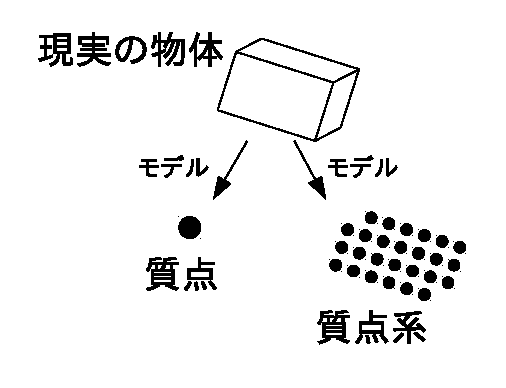
\includegraphics[width=5cm]{particle.eps}
    \caption{物体のモデル。大きさと形を無視できる場合は質点。そうでない
場合は質点系としてモデル化する(質点系では質点どうしの間に働く力も考える。
そうすることで物体がバラバラにならないように理論化できる)。}\label{fig:particle}
\end{figure}

\begin{q}\label{q:whatis_model}
モデルとは何か?
\end{q}

\begin{q}\label{q:whatis_particle}
質点とは何か?
\end{q}

モデルは科学のあらゆるところにある。例えば化学でいずれ学ぶ「理想気体」は現実
の気体のモデルのひとつである。

現実の現象や物体は往々にして複雑だが, それを複雑なままで見ているだけでは, 
仕組みはわからない。人間のしょぼい知性では複雑なものを理解できないのだ。
しかし複雑さをばっさり切り捨てて, 単純な状況に限定すると, 自然の仕組み
は人間ごときにも理解できることがある。だからモデルが必要なのだ。モデルの
力を借りて科学は進歩してきた。

ところが, いったん出来上がった科学を学ぶ我々は, 恩あるモデルの存在を忘れ, 
モデルに限って成り立つ法則が, 現実の複雑な現象にそのまま全面的に成り立つような
錯覚を起こしがちである。これは大変危険なことである。

\begin{exmpl} 君は小学校
で振り子を習っただろう。そこで振り子の周期は振れ幅に依存しない, と習った
はずだ。これを振り子の等時性\index{とうじせい@等時性}という。ところが, 
振り子の等時性は, 振り子の振れの角が十分に小さいという単純なモデルについてのみ成り立つ
近似的・限定的な性質である。振れの角が大きくなれば, 等時性は成り立たない。
実際, 振れの角が60度になれば周期は7パーセント程度長くなる
ことがわかっている。ちなみにこの「ずれ」は, 物理学と数学の理論で説明できる。
\end{exmpl}

君はこれから学ぶ科学の様々な事柄に対して, それがどのような限定の
中で成り立つかを注意深く理解しなければならない。そのためには, 
法則や理論の結論だけを丸飲みするのではなく, その理論の成立する
過程をきちんと理解し, それが現実の中の何をモデル化しているのか
理解しなければならない。
\hv



\begin{exq} 「筑波大学ギャラリー」(大学会館の中にある)を訪れて, 筑波大学にゆかりの
あるノーベル物理学賞受賞者に関する展示物の中から, あなたにとって最もインパクトの
あったものを報告せよ(その理由も含めて)。\end{exq}

\begin{exq} エンジニアや科学者にならない人も物理学を学ぶべきだろうか? 
君の考えを論じよ。\end{exq}


\section*{解答}

以下, 解答が無い問題は, 解答が略されているものである。\\

\noindent{\textbf{答}}\ref{q:basic_laws}\\
力学の基本法則: 慣性の法則・運動方程式・作用反作用の法則。万有引力の法則を加えることもある。
熱力学の三法則: 熱力学第1法則(エネルギー保存則)・熱力学第2法則(エントロピー増大の法則)・
熱力学第3法則(絶対エントロピーの法則)。
電磁気学の基本法則: マクスウェル方程式\footnote{それぞれの基本法則は, 別の形で言い換えることも
できる。特に, 熱力学第2法則やマクスウェル方程式の一部は, 別の形や名前で表現されることがある。}。
\vspace{0.2cm}

%\noindent{\textbf{答}}\ref{q:fake_science} 略
%\mv

% オッカムの剃刀とは何か?
\noindent{\textbf{答}}\ref{q:OccamsRazor}\\
基本法則として, 複数の候補があったとき, それらが同程度に有効であるなら, 
より単純なほうが正しいだろう, という考え方
\vspace{0.2cm}

% ある人の息子が, 「僕は将来, サッカー選手になりたい」と言う。
%\noindent{\textbf{答}}\ref{q:soccer}
%\begin{enumerate}
%\item $30\times30$で, 約1000人。正確には1067人だそうです(2010年Jリーグ発表)。
%\item $1000/5$で約200人。
%\item 1学年の児童は$100000000/100$で約100万人。このうち男子が半分として50万人。
%\item 200/50万で, 約0.0004。つまり1万人に4人, つまり2, 3千人にひとり。
%\end{enumerate}
%\vspace{0.2cm}

% 2011年現在, 日本の年間の国家予算は約100兆円である。
%\noindent{\textbf{答}}\ref{q:Japan_debt}
%\begin{enumerate}
%\item 年間国家予算は全借金の1/10程度。年間国連拠出金は全借金の1/40000程度。
%\item 年間国家予算はひとりあたり100万円程度。年間国連拠出金はひとりあたり250円程度。
%\end{enumerate}
%\vspace{0.2cm}

% 日本の平均年間降水量は1500mm程度である。
\noindent{\textbf{答}}\ref{q:Japan_rain_paddy}\\
日本の水田に, 1~m$^2$あたり1年間に必要な水量は, 0.5~kg$\times$3000~kg/kg=1500~kg。
水の密度は約1000 kg/m$^3$だから, これは1.5 m$^3$に相当。これを面積 1~m$^2$の地平面に
敷くと, 厚さは1.5~m, つまり1500~mmになる。一方, 日本の平均年間降水量は, 1500~mmなので, 
なんとか雨だけで足りる(計算上は)\footnote{現実は, もっと難しいことがいっぱいあるので, 
ほとんどの水田で灌漑が必要です。}。
\vspace{0.2cm}

% モデルとは何か?
%\noindent{\textbf{答}}\ref{q:whatis_model}
%現実のものや現象を単純化・抽象化してとらえ直し, 扱いやすくした近似的概念。
%\vspace{0.2cm}

% 質点とは何か?
%\noindent{\textbf{答}}\ref{q:whatis_particle}
%物体のモデルのひとつであり, 質量は持つが大きさは持たない, 点状の仮想的(理想的)な物体。
%\hv

\chapter{力の法則}

{\small 注: 数学リメディアル教材の第1・第2章を習得しておくこと。}

\section{力とは何か?}

小学校以来, 理科には何回も「力」が出てきたが, 諸君は「力」とは何か, わかっているだろうか?

「力」は, 有名な国語辞典である「広辞苑」(第六版電子版)では以下のように記されている:\\
(1) 自らの体や他の物を動かし得る, 筋肉の働き。(後略)\\
(2) 気力。精神力。根気。(後略)\\
(3) 能力。力量。実力。(後略)\\
...\\
(8) [理] 静止している物体に運動を起こし, また, 動いている物体の速度を変えようとする作用。(後略)\\

科学でいうところの「力」は, この(8)である。(1), (2), (3)とは全く
違うものである。

ところが, このことをきちんと理解せずに, 「力」を(1), (2), (3)のような
意味とごっちゃにして「理解」している人が多い。おそらく, 「物理が苦手」
「物理は嫌い」という人の多くがそうだろう。日常で使われる
(1), (2), (3)のイメージに引きずられて, ついつい「わかった気」に
なってしまっているのである。

余談だが, 力とエネルギーを混同している人も多い。後述するが, 
力とエネルギーは, 明確に別物である。「エネルギー」も日常でよく
出てくるので, なんか「わかった気」になってしまうのだろう。

科学では, このように, 「言葉にこだわる」姿勢が重要である。言葉に関する
間違った思い込みやあやふやな理解が, 理解を妨げるのである。

さて, 「広辞苑の(8)の説明を読んでもよくわからない」という人もいるだろう。
当然である。これを理解するには, 「運動」とか「速度」などを定義する必要
があるし, いろんな事例や観点について考えて納得していく必要があるからだ。

実は, この広辞苑の(8)は, 次章で詳述する「慣性の法則」と「運動方程式」を, 
部分的に言い換えたものである。これらの法則をもとに, 「力」が定義されるのだ。

「運動方程式」は, 数学リメディアル教材にも出てきたが, ざっくりいうと, 
力は質量と加速度の積に等しい, という法則である。その「意味」は次章で学ぶが, 
とりあえず, このことから力の「単位」がはっきりする。すなわち, SI単位系
では(SI単位系がわからない人はネットで検索するか, 「数学リメディアル教材」を
参照せよ), 質量の単位はkg, 加速度の単位はm~s$^{-2}$を使うので, 
その積は, kg~m~s$^{-2}$となる。これが, SI単位系における力の単位である。
これをN (ニュートン)\index{にゅーとん@ニュートン}と呼ぶ。
すなわち, 1~N=1~kg~m~s$^{-2}$である。

\begin{faq} {\small\textgt{力って, 本当に存在するのですか? 
目に見えないのでイマイチわかりません} ... 力というものが「本当に存在するかどうか」
は, 実はどうでもよいのです。「力」が実在すると考えれば, 宇宙の法則が矛盾なく簡潔に
整理できるのです。それが「力」の実在性の保証です。「そう考えれば全てつじつまが合う」
というのが, 物理学で認められる説得力であり, 正しさであり, 実在性なのです。
}\end{faq}

\begin{faq}{\small\textgt{結局, 「力」って何ですか?}
... あえて短く言えば, 物体の運動状態に変化をもたらすもの。}\end{faq}

\begin{faq}{\small\textgt{N (ニュートン)の定義がわかったようなわからないような...}
... kg~m~s$^{-2}$です。それ以外の何ものでもない。}\end{faq}
\mv

\begin{q}\label{q:4forece}
君は, 今まで「力」をどのように理解・認識していたか? 科学的に正確に
理解していたと言えるか? そうであれば, それはどのようなきっかけで
そうなったか? 正確に理解してはいなかったなら, なぜそうだったのか?
\end{q}


\section{4つの力}

%2011.4.1 ヤマサキ 脚注を変更。「田中さんの例」はむしろわかりづらいと感じました…。
自然界にはさまざまな力が存在するが, 根源的には, それらは以下の4つからなる
ということが, 物理学者達の長い苦闘の末, 明らかになっている:
\begin{itemize}
\item 重力
\item 電磁気力
\item 強い力(核力など)
\item 弱い力(ベータ崩壊など)
\end{itemize}
その他の力, たとえば摩擦力やバネの力などは, いずれもこれらの力から派生するものだ。
言い換えると, どのような力も,元をたどればすべてこの4つの力で説明できるのだ。

我々の身近な現象に関与する力は, ほとんどが重力または電磁気力だ。
「強い力」「弱い力」は, 「重力」や「電磁気力」と同じように, 
これ自体で科学的な専門用語である。何かの基準よりも強い(または弱い)
力を指すのではない。「強い力」は原子核の中で陽子や中性子を
同居させる力であり, これがなければ物質(元素)は存在できない。

「弱い力」は, 原子核のベータ崩壊(陽子が陽電子とニュートリノを発して
中性子に変わることなど)のときに関与する。その例として, 原発事故で
漏れ出した放射性セシウム$^{137}$Csが放射性バリウム$^{137}$Ba
に変わる崩壊がある。また, 放射性炭素$^{14}$Cが窒素$^{14}$Nに
変わる崩壊もベータ崩壊である。これは過去の生物遺体の年代測定に使われる。

\begin{q}\label{q:4forece}
自然界に存在する, 根源的な4つの力とは何か?
\end{q}
\hv


\section{力の一般的な性質}

ここで, 力の一般的な性質について学んでおこう。ここで述べるのは, その力
の起源が重力であれ電磁気力であれ何であれ, 例外なく成り立つようなことだ。
なお, 以後しばらく, 「物体」は質点と同義語と考えて欲しい。物体の大きさや
形を考えねばならないときは, 逐次, そのように言及する。

\begin{itemize}
\item 力には, 大きさと向きがある。つまり, 力はベクトルである。
\item ベクトルの数学に基づいて, 複数の力を足し合わせたり, ひとつの力を
複数の力に分解して考えてもよい。特に, ある物体に複数の力が働く場合, 結果的
には, その物体には, それらの力をベクトルとして足し算したもの(合力)\index{ごうりょく@合力}のみが
働くと考えてよい。
\item 物体が静止している場合, その物体に働く力(合力)はゼロである
\footnote{逆は必ずしも成り立たないことに注意せよ。すなわち, 働く力が
ゼロであっても物体は静止しているとは限らない。\textgt{力が働かなくても物体は
動いていることができるのだ}。(詳しくは慣性の法則のところで述べる)}。これを「力のつりあい」 \index{ちからのつりあい@力のつりあい}という。
これは後に述べる「慣性の法則」の特殊な場合だ。
\item 2つの物体A, Bにおいて, AがBに力を働くとき, AはBから, 同じ大きさで
逆向きの力を受ける。これを「\textgt{作用・反作用の法則}」\index{さようはんさようのほうそく@作用・反作用の法則}という。
\end{itemize}
\mv
ではこれから, いくつかの具体的な力について学んでいく。\\



\section{重力}\index{じゅうりょく@重力}

重力とは, 質量を持つ物体に働く力である。万有引力ともいう。
質量$M$と質量$m$をそれぞれ持つ2つの質点が距離$r$だけ離れて
いれば, その間に, お互いが引っ張る向きの力が生じる。
%(図\ref{fig:gravity})
\begin{comment}
\begin{figure}[h]
    \centering
    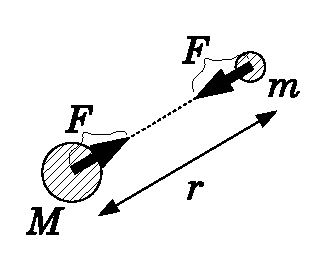
\includegraphics[width=5cm]{gravity.eps}
    \caption{2つの物体の間に働く重力。}\label{fig:gravity}
\end{figure}
\end{comment}
その力の大きさ$F$は以下の式を満たす:
\begin{itembox}{重力の法則}
\begin{eqnarray}
F=\frac{GMm}{r^2}\label{eq:gravity_univ}
\end{eqnarray}
\end{itembox}
これが重力だ。ここで, $G$は「万有引力定数」と呼ばれる定数で, 
\begin{eqnarray}
G=6.67\times 10^{-11}\text{ m}^3\text{ s}^{-2}\text{ kg}^{-1}
\end{eqnarray}
である。$G$の値は記憶しなくてもよいが, 式(\ref{eq:gravity_univ})は記憶せよ。

\eref{eq:gravity_univ}は, 英国の物理学者
アイザック・ニュートンが発見した。どうやって発見したのか? 
惑星の運行を説明するためにいろいろな数式を試行錯誤したのだ。ニュートンだけでなく, 
ガリレオ, ティコ・ブラーエ, ケプラー等の学者を含めた, 長い苦闘の成果である。

この式よりもさらに重力を一般的に説明する理論が「一般相対性理論」である。しかし
一般相対性理論は学類1年生には手に負えない理論なので, 我々は式(\ref{eq:gravity_univ})
を重力の基本法則(根源的な法則)とみなそう。\mv

ところで質量とはそもそも何だろうか? それは物体に重力を生じさせるような, 
物体の属性である。では重力とは何か? それは質量を持つ物体どうしに働く力だ。
この議論は循環論法だ。質量を定義するのに重力の概念が必要で, 
重力を定義するのに質量の概念が必要だ! こうして見ると, 世の中は
全てが論理的にすっきり説明できるものではなく, どこかで「そういうものが
あるのだ」と認めねば話がはじまらない。というわけで, 物体を特徴づける
量として質量というものが存在する, ということを天下りに認めよう。\mv

作用・反作用の法則のために, 質量$M$の物体が質量$m$の物体を引く力と, 
その逆, つまり質量$m$の物体が質量$M$の物体を引く力は, 互いに向きは逆だが, 
大きさは同じだ。質量の大きな物体が質量の小さな物体を引く力は, 
質量の小さな物体が質量の大きな物体を引く力と同じ大きさなのだ。

さて, 重力が最も活躍するのは, 天体の現象だ。星は, 重力に
よって物を引きつける。地球を含めて球状の星は, 重力に関しては, 
その中心に質量が集中しているとみなして扱える。例えば地球の
表面に立つ質量$m$の君に地球が及ぼす重力を考えるとき, 
$M$として地球の質量を, $r$として地球の半径を考えればよい。
これは自明なことではなく, 重力の法則をもとに数学的に証明
されることだが, ここではその詳細は述べない。気になる〜という
人は, まず大学の数学をしっかり勉強しよう。\mv

\begin{q}\label{q:grav_accel}
地球の半径を$r=6400$ km, 
地球の質量を$M=6.0×10^{24}$~kgとする。地表において質量$m=1.0$~kgの物体が受ける, 地球から
の重力が, 9.8 Nであることを示せ(有効数字二桁でよい)。ヒント: 単位を埋め込んで計算しないと
失敗するだろう!
\end{q}
\mv

\begin{comment}
ところで, 力はベクトル(大きさと向きを持つ量)\index{べくとる@ベクトル}なのだから, \eref{eq:gravity_univ}を, 
力の大きさだけでなく力の向きまできちんと表現できるような式に書き直すこともできる:
\begin{eqnarray}
{\mathbf F_{12}}=-\frac{G\,m_1 m_2({\mathbf r}_2-{\mathbf r}_1)}{|{\mathbf r}_2-{\mathbf r}_1|^3}\label{eq:gravity_univ_vect}
\end{eqnarray}
ここで, 2つの物体を, 物体1と物体2とし, ${\mathbf F_{12}}$は物体1が物体2に及ぼす重力(ベクトル), 
$m_1$, $m_2$はそれぞれ物体1と物体2の質量, ${\mathbf r}_1, {\mathbf r}_2$はそれぞれ物体1と物体2の
位置ベクトルである(大学ではベクトルを太字で書き表す)。
この式は, \eref{eq:gravity_univ}に「物体2から物体1へ向いた単位ベクトル」,すなわち
\begin{eqnarray}
-\frac{{\mathbf r}_2-{\mathbf r}_1}{|{\mathbf r}_2-{\mathbf r}_1|}
\end{eqnarray}
を付けた形になっている。\footnote{ベクトル${\mathbf r}_2-{\mathbf r}_1$(これは物体1を始点にして物体2まで伸びているベクトルである)を
そのベクトルの大きさ$|{\mathbf r}_2-{\mathbf r}_1|=r$で割って得られるベクトル(つまり${({\mathbf r}_2-{\mathbf r}_1)}/{|{\mathbf r}_2-{\mathbf r}_1|}$)が, 
「物体1から物体2へ向いた単位ベクトル」を表している。このベクトルをマイナス倍すると向きが逆になり, 結局この式は「物体2から物体1へ向いた単位ベクトル」を表すことになる。}
(図\ref{fig:gravity_vect})。
\begin{figure}[h]
    \centering
    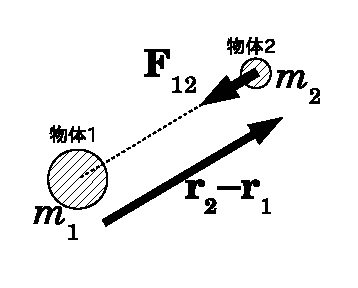
\includegraphics[width=5cm]{gravity_vect.eps}
    \caption{物体1が物体2に及ぼす重力${\bf F}_{12}$。}\label{fig:gravity_vect}
\end{figure}
\end{comment}

地表にある物体が地球から受ける重力について, もう少し考えよう。
$m$を地表の物体の質量, $M$を地球の質量とする。
地球中心から地表までの距離(つまり地球半径)を$r$とする。
地表の物体が地球から受ける重力の大きさ$F$は, 
\eref{eq:gravity_univ}から, 
\begin{eqnarray}
F=\frac{GM}{r^2}m\label{eq:gravity000}
\end{eqnarray}
となる。ここで, 物体を地球上のいろんなところに持って行っても, 
$G$, $M$, $r$はそれぞれ一定値とみなせる($r$だけは, 
高い山の上などに持って行くと微妙に変わるが, それでも
その変化はわずかである)。従って, 上の式の
\begin{eqnarray}
\frac{GM}{r^2}
\end{eqnarray}
は(ほぼ)定数とみなすことができ, これを$g$と置こう。すると
\eref{eq:gravity000}は, 
\begin{eqnarray}
F=mg\label{eq:gravity_earth}
\end{eqnarray}
と書ける。このとき, 比例係数$g$を「\textgt{重力加速度}」
\index{じゅうりょくかそくど@重力加速度}と呼ぶ(記憶せよ)。

実は, 上の説明はあまり正確ではない。例えば地球の形は完全な球形では
なく, 赤道付近がわずかに膨らんだ, 楕円体である(だから, 地球の中心に
質量が集中しているとみなすのは, 厳密にはダメである)。また, 地球
の密度は均一でないために, 地表の場所によって重力は大きかったり
小さかったりする。さらに, 実際に地表で感じられる重力には, 後で学ぶ
「遠心力」(地球の自転に起因する力)も加わる。従って, 実際は$g$の
値は場所によって微妙に異なる。これは生物資源学類としては注意が
必要なポイントだ。

\begin{q}\label{q:weight_calib} 化学実験では, 
試薬を量り取る時に電子天秤を使う。
電子天秤で量る重さは, その場の重力加速度に比例する。北海道大学(札幌市)
と筑波大学で同じ電子天秤を調整せずに使ったら, 重さの測定値は何%くらい違うか?
ヒント: 「電子天秤の校正 札幌 茨城」などをキーワードにして
インターネットなどで調べよ。\end{q}

これを意識しないと, 北大と筑波大で同じ実験をしたつもりでも, 
試薬の量が異なってしまい, 違う実験結果になりかねない!\mv

さて, なぜ$g$の呼び方に「加速度」という言葉がついているだろう? それは, $g$の次元を
考えればわかる。まず, \eref{eq:gravity_earth}より, $g=F/m$である。一方, 
さきほど学んだように, 
$F$のSI単位はN(ニュートン; kg~m~s$^{-2}$), $m$のSI単位はkgなので, $g$すなわち$F/m$
のSI単位は, kg~m~s$^{-2}$/kg = m~s$^{-2}$。従って, $g$は, 
加速度の次元を持つのだ。実際, 問\ref{q:grav_accel}の結果から, 
$m=1.0$~kgのとき$F=9.8$ Nだったので, 
$g=F/m$を計算すれば, 
\begin{eqnarray}
g= 9.8\,\,\text{m~s$^{-2}$}
\end{eqnarray}
である(この値は記憶せよ)。

ここでは$g$が加速度の次元を持つことを示したが, $g$は実際に加速度として
意味を持っている。君が地表付近で何かの物体を落としたら, その物体はほぼ
一定の加速度$g$で加速しながら落下するのだ。そのあたりの事情は, 後で詳しく述べる。

% ジオイド, 遠心力, はかりの校正

\begin{q}\label{q:what_is_g}
重力加速度とは何か?
\end{q}
\mv

\begin{q}\label{q:geostat_sat}
高度10,000~mの上空を飛ぶ旅客機と, 高度36,000~kmの上空を飛ぶ静止衛星には, 
それぞれ地表での重力の何パーセントの重力がかかるか? ヒント:
式(\ref{eq:gravity_univ})を使う。それぞれの$r$は地表での$r$の何倍になるか?
\end{q}
\mv

\begin{q}\label{q:moon_gravity}
月の質量は地球の質量の1/81.3, 月の半径は地球の半径の1/3.68である。月の表面で, 
月から受ける重力は, 地球の表面で, 地球から受ける重力の何倍か?
ヒント:式(\ref{eq:gravity_univ})を使う。$M$と$r$の両方が変わることに注意。
\end{q}
\mv

%\begin{q}\label{q:atm_pressure}
%地表での平均的な大気圧は, 1000 hPa程度である。1.0~m$^2$の地表面の上空には, 
%どのくらいの質量の大気が存在するか?
%ヒント:式(\ref{eq:gravity_earth})を使う。1.0~m$^2$の地表面の上空にある大気の
%質量を$m$とすれば, それにかかる重力$mg$が, 地表面での圧力を生む。なお重力は
%厳密には高さによって変わるが, ここではその変化を無視してよい。
%\end{q}\mv

\begin{faq}{\small\textgt{地球の中心に行けたら, 万有引力はどのように働くのでしょうか?}
... 全方向からの引力が打ち消しあって0になります。要するに「無重力」です。}\end{faq}\mv

\begin{faq}{\small\textgt{地球の質量は一定ですか? いろんな反応が
起こって絶えず変わっているイメージです。}
... 地球には隕石等が宇宙から飛来して質量を増やす一方, 地球大気から(地球の重力を
ふりきって)宇宙に飛散する分子や原子もあり, 質量を減らす。そんなこんなで, 地球の質量は, 
絶えず微妙に増減しているでしょう。}\end{faq}\mv

\begin{faq}{\small\textgt{万有引力はどんな物体の間にも
はたらいているのですか?例えば人と人の間とか。}
... 質量を持つ物体ならどんな物体の間にも働いています。もちろん人と人の間にも働いていますよ。}\end{faq}
\hv



\section{クーロン力}\label{sect:CoulombForce}\index{くーろんりょく@クーロン力}
次に, 電磁気力について考えよう。電磁気力とは, 「電荷」を
持つ物体に働く力のことだ。

物質を構成するのは原子核や原子, イオンなどであり, それらを構成するのは, 
電子や陽子, 中性子, 中間子など, 「素粒子」と呼ばれる微細な粒子だ。
なぜだかわからないが, それぞれの素粒子には, \underline{電荷}
\index{でんか@電荷}という, 固有の性質(物理量)がある。
電荷の性質として, 
\begin{itemize}
\item 電荷は正と負という符号のある量である。
\item 電子1個と陽子1個は, 同じ大きさで逆の符号の電荷を持っている。
\end{itemize}
ということが知られている。これらがなぜなのかは, 根本的には
わかっていない。そのようにこの世界は作られているのだとしか
言う他はない。そして, 電子1個や陽子1個が持つ電荷の大きさを
$1.602\times 10^{-19}$~Cとする(Cというのは電荷の単位であり, 
「クーロン」と呼ぶ。SI基本単位で表せば, 1 C=1 A~sだ)。
これを\underline{電荷素量}\index{でんかそりょう@電荷素量}と呼び, 
$q_e$とあらわす。$q_e$は, 有効数字4桁では, 
$q_e=1.602\times10^{-19}\text{ C}$である(記憶せよ)。
電子の電荷を$-q_e=-1.602\times10^{-19}\text{ C}$, 
陽子の電荷を$+q_e=1.602\times10^{-19}\text{ C}$とする。

原子核や原子, イオン, 分子などの粒子や, もっと大きい物体は, 
それを構成する素粒子の持つ電荷の総和(正の値と負の値を加えて
差し引きした量)を電荷として持つ, と約束する。例えば, 
水素原子は1個の陽子と1個の電子から構成されるが, 陽子と
電子の電荷は同じ大きさで逆符号なので, その総和は0である。
従って, 水素原子の持つ電荷は0である, とみなす。正の電荷
と負の電荷のどちらかが多いときだけ, その粒子は0以外の
電荷を持つことになる。粒子や物体が0以外の電荷を持つときは, 
その粒子や物体は「帯電している」という。帯電している粒子の
ことを荷電粒子という。電子や陽子, 原子核, イオンなどは
荷電粒子だ。荷電粒子のことを電荷ということもある。\mv

さて, 電磁気力のひとつを紹介しよう。「粒子1」と「粒子2」という2つの荷電粒子がある
とき, それらの間には, 電荷に応じて, お互いを引っぱる
向きの力(引力)またはお互いを遠ざける向きの力(斥力)が働く。その引力または
斥力の大きさを$F$とすると, $F$は以下の式を満たす:
\begin{itembox}{クーロンの法則}\index{くーろんのほうそく@クーロンの法則}
\begin{eqnarray}
F=\frac{k\,q_1\,q_2}{r^2}\label{eq:coulomb}
\end{eqnarray}
\end{itembox}
ここで, $q_1, q_2$は粒子1と粒子2がそれぞれ持つ電荷, $r$は粒子間の距離である。
$k$は定数で, 有効数字4桁では, $k=8.987\times 10^{9}$ N~m$^2$ C$^{-2}$だ。
この式(\ref{eq:coulomb})を, クーロンの法則 (Coulomb's law)と呼び, このように
記述される電磁気力をクーロン力 (Coulomb force)と呼ぶ。クーロンというのは, この法則
を見つけた物理学者の名前だ。$k$の値は記憶しなくてもよいが, 式(\ref{eq:coulomb})
は記憶しよう。\mv

クーロン力は, 電荷を持つ物体に働く力だ。一方, 
重力は, 質量を持つ物体に働く力であった。興味深いことに, これらの
数学的な表記, すなわち\eref{eq:coulomb}と\eref{eq:gravity_univ}
は, 互いによく似ている。従って, 重力に関して成り立つ議論, 特にその数学的な扱いは, 
クーロン力にも通用することが多いし, その逆も然りである。

\begin{faq}{\small\textgt{性質も似ているのでしょうか? この2つの式は統合できるのでは?}
... 地球中心で重力がゼロになるように, 一様に帯電した球の中心では電場がゼロになる, などの, 
よく似た性質があります。しかし, これらの式の統合には, 誰も成功していません。}\end{faq}\mv

さて, 上述のように, 電荷には, \textgt{正電荷}と\textgt{負電荷}の二種類がある。$q_1$とか$q_2$は
プラスやマイナスの値をとり得るのだ。そして, $q_1$と$q_2$が同符号(両方ともプラス, 
もしくは両方ともマイナス)のとき, 式(\ref{eq:coulomb})から$F$はプラスになり, そのとき, 
2つの粒子の間には, 斥力(互いに遠ざける力)がはたらく。一方, $q_1$と$q_2$が異符号
(片方がプラスで片方がマイナス)のとき, $F$はマイナスになる。力の大きさがマイナスに
なるのは奇妙だが, このマイナスは, 2つの粒子の間に, 引力(互いに引き合う力)が
はたらくことを意味する (ここが重力との大きな違いだ。重力には
引力しかない。また,質量にはプラス(またはゼロ)しかない)。つまり, 
\eref{eq:coulomb}は力の大きさだけでなく向き(引力か斥力か)も表現している。

\begin{comment}
このあたり
の事情も考慮して, \eref{eq:coulomb}を, きちんと力の向きまで完全に記述できる
ように書くと, 次式のようになる:
\begin{eqnarray}
{\mathbf F_{12}}=k\,\frac{q_1 q_2({\mathbf r}_2-{\mathbf r}_1)}{|{\mathbf r}_2-{\mathbf r}_1|^3}\label{eq:coulomb_vect}
\end{eqnarray}
%2011.4.2 ヤマサキ 「ベクトルで表した重力の式についての変更」と連動して変更。
ここで, ${\mathbf F_{12}}$は粒子1が粒子2に及ぼす力(ベクトル), ${\mathbf r}_1, {\mathbf r}_2$はそれぞれ
粒子1と粒子2の位置ベクトルである。
このような式の形になる理由は, 重力のとき(\eref{eq:gravity_univ_vect})の事情と同様だ。\mv

\begin{faq}{\small\textgt{なぜ$q_1q_2<0$のとき${\bf F}_{12}$は引力で, 
$q_1q_2>0$のとき${\bf F}_{12}$は斥力になるのですか?}
... \eref{eq:coulomb_vect}を見ると, ベクトル${\bf F}_{12}$が, 
ベクトル${\mathbf r}_2-{\mathbf r}_1$を何倍かした形になっています。
その係数$k\,q_1\,q_2/|{\mathbf r}_2-{\mathbf r}_1|^3$の正負
は$q_1q_2$の正負で決まります。これが正のときは, ${\bf F}_{12}$は
${\mathbf r}_2-{\mathbf r}_1$と同じ向き, すなわち粒子1から粒子2までの
ベクトルと同じ向きです。すなわち, 粒子1が粒子2に及ぼす力は, 粒子2を
押しのける方向に働く, というわけです。$q_1q_2<0$のときはその逆。}\end{faq}
\end{comment}

\begin{q}\label{q:coulomb_law}
クーロンの法則とは何か?
\end{q}
\mv

\begin{q}\label{q:element_charge}
電荷素量とは何か?
\end{q}
\mv

\begin{q}\label{q:elec_grav_compare}
互いに1.0~m離れたところに存在する2個の電子の間には, 
クーロン力と重力の両方が働く。そのクーロン力を$F_e$, 重力を$F_g$とする。
\begin{enumerate}
\item $F_e$の大きさを求めよ。
\item $F_g$の大きさを求めよ。ただし, 電子の質量$m_e$は, $9.1\times10^{−31}$~kgである。
\item $F_g$は$F_e$の何倍か?
\end{enumerate}
\end{q}\mv


\section{電場と磁場}

さて, 電磁気力には, クーロン力だけでなく, 磁気的な力(磁力)もある。
クーロン力は, 荷電粒子が静止していようが運動していようが, 
無関係に働く。ところが磁力は, 荷電粒子が運動しているときにのみ働く。
それらを含めて正確に言えば, 次のようになる(今は詳細は理解しなくてよい):

電磁気力とは, 荷電粒子の電荷$q$に比例するような力であり, それは何らか
の2つのベクトル${\bf E}$, ${\bf B}$を用いて, 
\begin{eqnarray}
{\bf F}=q{\bf E}+q{\bf v}\times{\bf B}\label{eq:LorentsForce}
\end{eqnarray}
と書けることがわかっている(${\bf v}$は荷電粒子の速度)。
このような形で荷電粒子に力を及ぼすようなベクトル${\bf E}$
と${\bf B}$を, それぞれ\underline{電場}\index{でんば@電場}
と\underline{磁束密度}\index{じそくみつど@磁束密度}
と呼ぶ(定義)。

ここで$\times$という記号が出てきた。これはただの掛け算ではなく, 
ベクトルの「外積」というものである。今はこれは理解できなくてもよい
(知りたい人は数学リメディアル教材を参照)。「そんなものがあるのか」
という程度の理解でOK。そして, ある定数を磁束密度にかけたものを
\underline{磁場}\index{じば@磁場}という(詳細は割愛する)。\mv

電場と磁場は不可分であり, 互いに影響を及ぼしあうから, これらを
まとめて語るのだ。その基本法則を「マクスウェル方程式」という。これは本書では
扱わない。それを理解するには, 「ベクトル解析」\index{べくとるかいせき@ベクトル解析}
という高度な数学(ベクトルの微分と積分に関する数学)が必要であり, 
今の君には難しい。また, 特殊相対性理論というものでは, 
電場と磁場が統一されるのだが, それも難しすぎるので
本書では学ばない。\mv

\begin{q}\label{q:Coulomb_EF} 1個の電子から1.0~mの距離にある点
での電場の大きさを求めよ。ヒント: 今は${\bf B}$を考えなくてよい。\end{q}\mv

\begin{faq}{\small\textgt{高校で磁力を習った時, フレミングの左手の法則
というのがありましたが...}
... \eref{eq:LorentsForce}があればフレミングの左手の法則は不要
です。
\eref{eq:LorentsForce}はフレミングの左手の法則を包含し, それよりも
一般性の高い, 強い式なのです。ただしこれを使いこなすには「外積」を
理解する必要があります。がんばって数学を勉強してください!}\end{faq}

\begin{faq}{\small\textgt{磁力は電荷を持った粒子が運動しているときに働く
とのことですが, 静止した磁石同士にはたらく磁力はどうなんですか?}
... 磁石の中では電子のスピンというもののせいで, 電流が流れているのです。
それに磁力がかかるのです。}\end{faq}

\begin{faq}{\small\textgt{「今は理解できなくてよい」のなら, ここで教えなくても
いいんじゃないですか?}
... 「そんな言葉を聞いたことがある」「そんな式を見たことがある」
というのが大事なのです。そういうのが「伏線」になり, 皆さんの学習効率
を高めるのです。}\end{faq}\mv


\section{張力}
ここまでは, 上で述べた根源的な4つの力について学んだ。
ここからは, この4つの力から派生する力について学ぼう。
まずは「張力」という力だ。

例として, 君が天井から垂れ下がったロープに吊り下がって静止しているとしよう
(簡単のため, ロープの質量は無視する)。
ロープに1箇所でも弱い部分があればロープは切れて君は落下するだろう。従って, 
君に働く重力は, ロープの全ての箇所にも働いていることがわかる。
\begin{figure}[h]
    \centering
    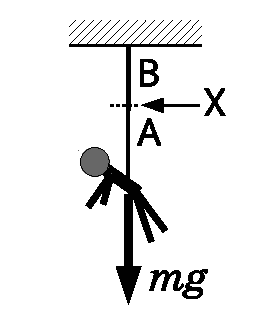
\includegraphics[width=5cm]{string.eps}
    \caption{ロープに吊り下がる人}\label{fig:string}
\end{figure}

ではロープの任意の1箇所Xを考えよう。そこより下の部分をロープA, そこより上の部分を
ロープBと呼ぼう。本来はロープAとロープBはXで繋がっていて1本のロープなのだが, 
便宜上, そう名づける。

さて, ロープAはロープBを下向きに引っ張っている。これは直感的に明らかだ。
一方, 同時にロープBはロープAを上向きに引っ張っている。
これは作用・反作用の法則に従えば明らかである(ロープAを「物体A」, ロープBを「物体B」として考えればよい)。
ロープBがロープAを上向きに引っ張っているというのがわかりにくければ, 次のように考えてもいい:
仮にロープBがロープAを上向きに引っ張っていないとすると, 
「君の体とロープAを合わせた物体」に働く力は重力のみである。しかし今, 
「君の体とロープAを合わせた物体」はロープに吊られて「静止」している。
静止しているからには, 「力のつりあい」が成り立たなくてはならない。
従って, ロープBはXにおいてロープAに「君に働く重力と同じ大きさで, 反対向き(上向き)の力」
を及ぼしていると考えざるを得ない。

これらの考察の結論(「君に働く重力と同じ大きさの力は, ロープの任意の箇所(つまり全ての箇所)
にも働いている」「ロープの任意の箇所では, そこを挟んで互いに逆向きで同じ大きさの力が働いている」)から, 
次のような結論が得られる: すなわち, ロープの端に力が働く場合, それと同じ大きさの力が, 
ロープの任意の箇所において, その箇所を挟んで互いに逆向きに働く。

このような力を\textgt{張力}と呼び, 慣習的に$T$で表す。張力には以下のような性質がある
(というか, 以下が張力の定義である):
\begin{itemize}
\item 張力は糸状の物体(ロープなど)に働く。
\item 張力は糸の各箇所で, 糸(の接線)に平行に働く。
\item 糸にかかる摩擦力や, 糸自体の質量にかかる重力が無視できる限り, 張力の大きさは糸のどこでも同じである。
\item 張力は, 引っ張りの向きにしか働かない。つまり, 糸を任意の箇所で2つに分割すると, 両者は互いに引き合う
力を及ぼす(互いに押し合う力は及ぼさない)。
\end{itemize}

ところで, 不幸にしてXが弱かったらどうなるだろう? ロープはXで重力に耐えきれずに, 次第に伸びて, 最後には切断されてしまう。
そうなると, 君に働く重力に抗っていた力は消えてしまい, 君は落下してしまうことになる。
ただし, その場合でも, ロープが完全に切断される寸前まで張力は存在するのだ。

\begin{q}\label{q:force_rope1}
図\ref{fig:string2}のように, 片端が壁にとりつけられた綱を力$F$で引く場合(上)
と, 両端を力$F$で引く場合(下)では, 綱にかかる張力の大きさは, どちらも$F$で等しい。このことを
説明せよ。
\begin{figure}[h]
    \centering
    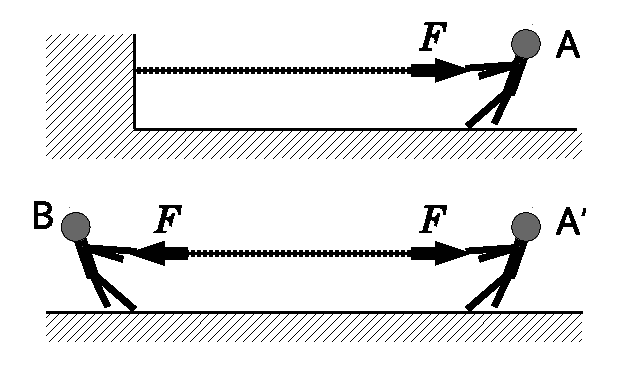
\includegraphics[width=7cm]{string2.eps}
    \caption{壁対人の綱引き(上)と, 人対人の綱引き(下)}\label{fig:string2}
\end{figure}
\end{q}

%
\begin{q}\label{q:force_rope3}
図\ref{fig:string3}のように, 質量$m$の君は, 天井に吊り下げられた滑車に
通されたロープの片端を体に結び, もう片端を手に持って, 自らの力で自らの体を
持ち上げようとしている。君の手がロープを引く力は$mg/2$であることを示せ(つまり, 
体重の半分の力で君は自分を持ち上げることができるのだ)。
\begin{figure}[h]
    \centering
    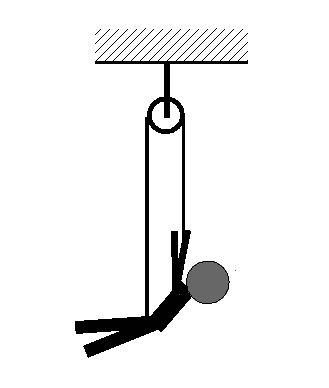
\includegraphics[width=4cm]{string3.eps}
    \caption{自力で上昇しようとする人}\label{fig:string3}
\end{figure}
\end{q}
\mv

%
\begin{q}\label{q:force_rope4}
図\ref{fig:string4}のように, 君は, 天井から固定された滑車Aと, 自由に
上下できる滑車B(動滑車)を利用して, 質量$m$の物体をロープで持ち上げようと
している。滑車の質量は無視し, ロープと滑車の間の摩擦は無いものとする。ロープは
一端が天井に固定され, 滑車Bと滑車Aを通って, もう一端が君の手に握られている。
君がロープを引っ張るのに必要な力は, 
$mg/2$であることを示せ。ヒント:ロープにかかる張力を$T$とすると, 滑車Bには上向き
に$2T$の力が働く。
\begin{figure}[h]
    \centering
    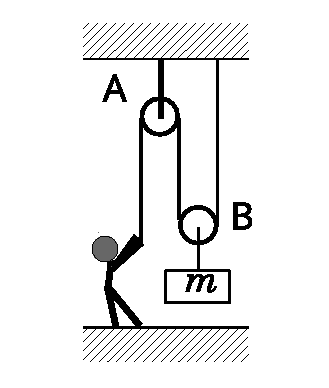
\includegraphics[width=5cm]{string4.eps}
    \caption{動滑車を使って物を持ち上げる}\label{fig:string4}
\end{figure}
\end{q}

\begin{faq}{\small\textgt{要するに天井と人が半分ずつ引っ張っているということ?}
... そうです。}\end{faq}\mv


問\ref{q:force_rope4}の考え方を援用すれば, 図\ref{fig:string4_iketeru}のように, 
動滑車の数を増やせば増やすほど, 小さな力で物を持ち上げることができる, ということがわかるだろう。
\begin{figure}[h]
    \centering
    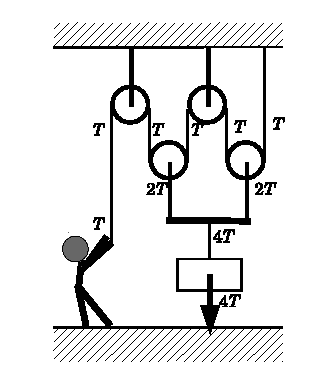
\includegraphics[width=6cm]{string4_iketeru.eps}
    \caption{2個の動滑車を使えば, 必要な力は1/4になる。}\label{fig:string4_iketeru}
\end{figure}

%
\begin{q}\label{q:force_rope5}
君の手がロープを引っ張るとき, その力の根源は何か?自然界に存在する4つの
根源的な力に帰着して説明せよ。
\end{q}
\hv



\section{圧力と応力}

化学などでは「圧力」\index{あつりょく@圧力}がよく出てくる。
圧力は, 面に垂直にかかる力を, 面積で割ったもの
(すなわち, 単位面積当たりの力)である。

圧力は, 「面に垂直」以外の方向まで含めて, 「面にかかる力を面積で割ったもの」
をあらわす時は, 「応力」\index{おうりょく@応力}という。圧力は応力の一種である。
特に, 面に平行にかかる力を面積で割ったものを, 「せんだん応力」という。それに
対して, 圧力のことを「垂直応力」ともいう。

当然ながら, 圧力や応力の単位は, 力の単位を面積の単位で割ったものである。
SI単位系では, N/m$^{2}$である。N=kg~m~s$^{-2}$なので, これはkg~m$^{-1}$~s$^{-2}$
とも書ける。この単位のことをPa (パスカル)と呼ぶ。

圧力は力ではない。圧力に面積を掛けたものが力である。

力はベクトルだが, 圧力は, 多くの場合, ベクトルでなくスカラーとして表現する。
その理由は, ここでは述べない。とりあえず「その方が便利だから」ということで
納得しておいてほしい。以下でも, 圧力やせん断応力はスカラーとして扱う。

\begin{exmpl} 底面積が$A=$0.50~m$^2$で質量が$m=$3.0~kgの箱がある。
この箱を地面に置いた時, 箱の直下の地面にかかる圧力を求めよう。

重力加速度を$g$とする。箱の重さは$mg$であり, これが地面にかかる力。
従って圧力は, $mg/A=3.0$~kg$\times 9.8$~m~s$^{-2}/$(0.50~m$^2)\fallingdotseq 60$~kg~m$^{-1}$~s$^{-2}\fallingdotseq 60$~Pa。(例おわり)
\end{exmpl}

\begin{q} 上の例で, 箱の質量はそのままで, 
箱の底面積が1/10になると(つまり0.050~m$^2$になると), 圧力はどうなるか?
\end{q}

\begin{q}\label{q:pressure_shoes} 君が立っている時, 君の足の裏の
直下の地面にはどのくらいの圧力がかかっているかを見積もれ。君の体重や
足の裏の面積などは適当な数値を仮定せよ(多少の嘘はOK)。
\end{q}

\begin{q}\label{q:pressure} 地表面での大気圧はおよそ1000~hPaである。
数学リメディアル教材で学んだように, hPaのhは「ヘクト」であり, 100を意味する。
\begin{enumerate}
\item 面積1~m$^2$の地表には, どのくらいの力がかかっているか?
\item 面積1~m$^2$の地表の真上には, どのくらいの質量の大気があるか?
\end{enumerate}
\end{q}

\begin{faq}{\small\textgt{人間が地上にいるとき, 大気の圧力に
押しつぶされないでいられるのは, どのような力が内側からはたらいて
いるのですか? また, もし人間が体ひとつで圧力のあまりかからない
ものすごく高い場所に行ったとしたら, その人は破裂するのでしょうか?}
... 人体の大部分は水であり, そもそも(液体の)水は圧力がかかってもあまり
変形しません。それが「つぶれない」ことのひとつの理由。また, 肺に空気がありますが, 
鼻を介して肺は外気とつながっているのでその圧力は基本的に外気の圧力(大気圧)と同じ。
従って, 肺の空気は大気圧と同じ圧力で押し返すから肺もつぶれない。ただし, 人間が
体ひとつで潜水する場合は, これが成り立ちません。特に, 水圧のために肺の空気が圧縮
されます。そのため, ある程度以上の深さに潜ると, 人間の体に働く浮力(それは体積に
比例する)が小さくなって, 人間の体は勝手に沈んでいくそうです(先日, テレビでやって
いました)。

逆に気圧の低いところ, 特に真空等に行ってしまうと, 体液が沸騰します(一般に, 
圧力が低くなると液体の沸点は下がる)。}\end{faq}
\mv


\section{弾性力(フックの法則)}

%2011.4.2 ヤマサキ 後に「バネの自然長」という言葉が使われているけど,それまでに説明がされてないので少し追加。
次に, バネについて考えてみよう。バネの自然状態での(力がかかってないときの)長さを「バネの自然長」と呼ぶことにする。
我々の日常経験から, バネを伸ばせば伸ばすほど強い力が働くことは自明だろう。
バネみたいに, 変形させると力を生じる物体について, 変形(変位)$x$と力$F$の関係を
関数$F(x)$で書くと, その関数がどんなものなのかはわからなくても, とりあえず
微分の定義から, 
\begin{eqnarray}F(x+dx)=F(x)+F'(x)dx\end{eqnarray}
となる($dx$は微小量)。ここで, $x=0$がつりあいの位置(バネの片端を固定し, 
自然状態に保ったときのもう片端の位置)に来るように座標を
とれば, $x=0$では力は働いていないから, $F(0)=0$となる(図\ref{fig:spring}の上の図)。
すると上の式は, 
\begin{eqnarray}
F(0+dx)&=&F(0)+F'(0)dx
\end{eqnarray}
つまり
\begin{eqnarray}
F(dx)&=&F'(0)dx
\end{eqnarray}
となる。この式は微小な量$dx$にしか厳密には成立しないけど, $x$が十分に小さい範囲に
限定して, $dx$を$x$と置き換えても近似的に成り立つと仮定すれば, 
\begin{eqnarray}
F(x)=F'(0)x\label{eq:HookeLaw3}
\end{eqnarray}
となる。ここで$F'(0)$の符号について考えてみよう。バネの力というものは, 伸ばせば
縮まる方向に, 縮めれば伸びる方向に働く。つまり, 変形(変位)と逆向きに働く。
従って, $x$が正なら$F$は負, $x$が負なら$F$は正である。従って, \eref{eq:HookeLaw3}に
おいて$F'(0)$は負であるはずだ。そこで, 形式的に$F'(0)$を$-k$と書き換えよう。このとき
$k$は正の定数である。すると\eref{eq:HookeLaw3}は, 
\begin{itembox}{フックの法則}
\begin{eqnarray}
F=-kx\label{eq:Hooke}
\end{eqnarray}
\end{itembox}
となる。ここで, $F$は, バネから受ける力, $x$はバネの伸び, $k$は\textgt{バネ定数}
\index{ばねていすう@バネ定数}と言われる定数である。これをフック(Hooke)の法則
\index{ふっくのほうそく@フックの法則}という。
\begin{figure}[h]
    \centering
    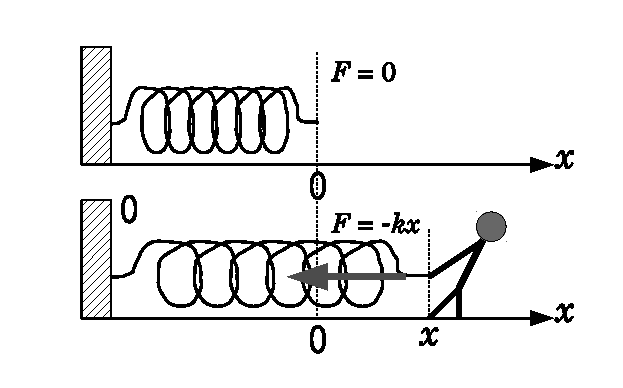
\includegraphics[width=8cm]{spring.eps}
    \caption{Hookeの法則}\label{fig:spring}
\end{figure}

このような数学的な考え方を線型近似と言う(数学リメディアル教材参照)。
要するに, フックの法則は, 力と変形(変位)の関数の線型近似式に過ぎず, バネ定数とは
その関数の微分係数(の絶対値)に過ぎない。

\eref{eq:Hooke}から明らかに, バネが伸びるほど力の大きさは大きくなる。繰り返すが, 
右辺のマイナスは, バネの伸びの方向($x$の符号)と力の方向($F$の符号)が逆だよ, 
ということを示す。バネは伸びると($x$が正だと), 縮もうとする力, つまりひっぱる
力を生じるから$F$は負になる。一方, バネは縮むと($x$が負だと), 伸びようとする力
を生じるから$F$は正になる。

\begin{q}\label{q:Hooke_law} 
\begin{enumerate}
\item フックの法則とは何か?
\item バネ定数とは何か?
\item バネ定数のSI単位は?
\end{enumerate}
\end{q}
\mv

さて, この「法則」は, 万有引力の法則やクーロンの法則よりも, ずっと一般性の
低い「しょぼい」法則である。フックの法則は, 限定的な例にしか成り立たない経験則
に過ぎない。実際, バネをどんどん伸ばすと, まっすぐな針金になってしまって, 
それ以上は伸びようがない。無理に伸ばすと, ぶちっと切れてしまう。従って, 
フックの法則は, バネの伸び($x$)がゼロに近いときにしか成り立たない。また, 
そもそもなぜこのような力が生じるかというと, バネの中の物質を構成する原子や
分子どうしが引き合う力(主に電気力)がその根源にあるからである\footnote{ただし, 
基本法則からフックの法則を導くのは, 簡単ではない。}。

式(\ref{eq:Hooke})は, バネだけに成り立つのではなく, 一般に, 多くの物質や
物体に成り立つ。例えば橋を構成する鉄骨は, 荷重や自重によって伸び縮みする。
フックの法則に従うような力を\textgt{弾性力}\index{だんせいりょく@弾性力}
と呼ぶ。弾性力によって変形する物体を\textgt{弾性体}\index{だんせいたい@弾性体}
と呼ぶ。そう考えると, フックの法則は, 「法則」という
よりもむしろ, 弾性力や弾性体の定義である, とも言えるだろう。


\begin{q}\label{q:elasticity}
弾性力とは何か?弾性体とは何か?
\end{q}
\mv

\begin{q}\label{q:plasticity}
弾性体ではない存在として, 「塑性体」というものがある。塑性体とは何か, 調べよ。
\end{q}
\mv

\begin{faq}{\small\textgt{高校ではフックの法則は$F=kx$で習ったのですが, 
$F=-kx$との考え方の違いは?}
... $F=kx$と書くときは, 力の大きさだけを考えていますが, $F=-kx$の場合
は力の向きまで考えています。}\end{faq}\mv

さて, 例として, バネ定数$k$のバネを天井からつるし, その先端に質量$m$の物体を
吊り下げて静止させる。バネ自体の質量は無視しよう。では, バネはどのくらい
伸びるだろうか?

鉛直下向きに$x$軸をとり, 物体をつるす前のバネの先端の$x$座標を0とする。
物体をつるしてバネが$x$だけ伸びたとき, 物体にかかるバネの弾性力は$-kx$, 
物体にかかる重力は$mg$である(ただし$g$は重力加速度)。前節で述べた, 
「物体が静止している場合, その物体に働く力(合力)はゼロである」という
法則(「力のつりあい」)から, この物体が静止するにはこの2つの力の和がゼロでなければならない。
従って, 
\begin{eqnarray}
-kx+mg=0
\end{eqnarray}
従って, $kx=mg$, 従って, 
\begin{eqnarray}
x=\frac{mg}{k}\label{eq:x_mg_k}
\end{eqnarray}
である。これがバネの伸びである。


\begin{q}\label{q:spring_moon}
同じ物体と同じバネを月面に持っていって同様の実験をするならば, 
バネの伸びは地球上の何倍になるか?ヒント:地球上の重力加速度に相当する
ものは, 月面上ではどうなるだろうか?
\end{q}
\mv

\begin{q}\label{q:spring_double_parallel}
図\ref{fig:spring_serial}左のように, バネ定数$k$のバネを2本, 平行に
ならべて天井からつるし, その先端をつなげて, そこに質量$M$の物体を吊り下げて
静止させる。バネは$Mg/(2k)$だけ伸びることを示せ。この状況で2本のバネをあわせて
1つのバネとみなすとき, そのバネ定数は$2k$となることを示せ。ヒント:重力$Mg$を, 
2本のバネで分担する。バネ定数を求めるには, バネ定数の定義を思い出すこと。(バネの並列)
\end{q}
\mv

\begin{q}\label{q:spring_double_series}
図\ref{fig:spring_serial}右のように, バネ定数$k$のバネを2本, 
縦につなげて天井からつるし, その先端に質量$M$の物体を吊り下げて静止させる。
バネは$2Mg/k$だけ伸びることを示せ。この状況で2本のバネをあわせて1つのバネと
みなすとき, そのバネ定数は$k/2$となることを示せ。ヒント:こんどは重力を分担
できない。上のバネにも下のバネにも, $Mg$の力がかかる。(バネの直列)
\mv
\begin{figure}[h]
    \centering
    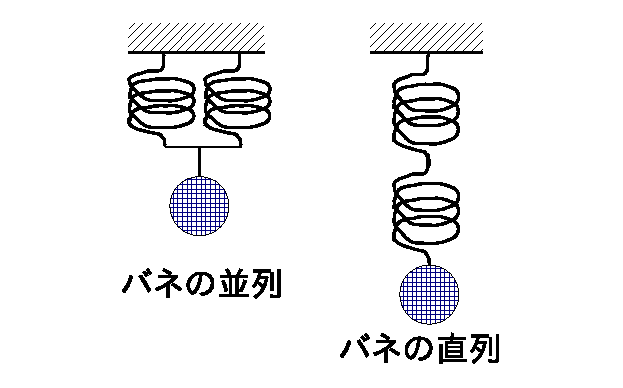
\includegraphics[width=7cm]{spring_serial.eps}
    \caption{バネの並列と直列}\label{fig:spring_serial}
\end{figure}
\end{q}

%
\begin{q}\label{q:spring_big}
バネ定数$k$のバネを$a$本だけ縦につないだものを$b$本だけ束ねて
大きなバネを作ると, そのバネ定数は$bk/a$となることを示せ。ヒント:
$n$本の直列を$m$本だけ並列。
\end{q}
\mv


断面積$A$, 長さ$L$の棒Xのバネ定数を考える。この棒を, 無数の小さい
(細くて短い)棒の集合(それぞれが弾性体)と考えれば, 棒Xの断面積は, 
小さい棒の並列の本数に, 棒Xの長さは, 小さい棒の直列の本数に, それぞれ比例
するので, 棒Xのバネ定数$k$は, $A/L$に比例する。そこで, 
\begin{eqnarray}
k=E\frac{A}{L}
\end{eqnarray}
と書く。このとき$E$を\textgt{ヤング率}\index{やんぐりつ@ヤング率}と呼ぶ。
ヤング率は物質に固有の定数(物性値)である。

\begin{q}\label{q:YoungModulus} 
\begin{enumerate}
\item ヤング率のSI単位は?
\item 鉄のヤング率を調べよ(「理科年表」\footnote{国立天文台(編)「理科年表」丸善。
毎年, 最新版が出ているが, 基本的なデータはそんなに頻繁には変わらないので, 昔の年のものを参照しても大丈夫。}などを使え)。
\item 長さ10~m, 直径2.0~mmの鉄線の先に10~kgの物体を吊り下げると, 鉄線はどのくらい伸びるか?
\item (3)で直径を半分(1.0~mm)にするとどうなるか?
\item (3)で鉄のかわりに銅を使うとどうなるか?
\end{enumerate}
\end{q}
\mv

ヤング率を使うと, フックの法則は以下のように書ける:
\begin{eqnarray}
F=-E\frac{A}{L}x
\end{eqnarray}
従って, 
\begin{eqnarray}
\frac{F}{A}=-E\frac{x}{L}
\end{eqnarray}
左辺の$F/A$は単位面積あたりの力で, 以前述べたように
「\textgt{応力}」\index{おうりょく@応力}と呼ぶ。「圧力」と呼んでもよさそうなもの
だが, この手の話題では圧力ではなく応力という言葉を使う。

右辺の$x/L$は単位長さあたりの伸びであり, 
「\textgt{ひずみ}」\index{ひずみ@ひずみ}と呼ぶ。応力を$\sigma$, 
ひずみを$\epsilon$と書くと, 上の式は, 
\begin{eqnarray}
\sigma=E\epsilon
\end{eqnarray}
と書ける(符号はとりあえず無視した)。これもフックの法則のひとつの表現である。
ここで示したフックの法則は, 1方向の伸びと, それと同方向のひずみとの間の関係で
あったが, それ以外にも, 様々な方向の応力と様々な方向の歪みに関しても同様の
関係が成り立つ。それを総称してフックの法則と呼ぶ。ただし, それをきちんと
表現するには, テンソル\index{てんそる@テンソル}という数学(「行列」の拡張版
みたいなもの)が必要であり, それは2年生以降に学ぶ。\mv

\begin{q}\label{q:stress_strain} 
\begin{enumerate}
\item 応力のSI単位は?
\item ひずみのSI単位は?
\end{enumerate}
\end{q}\mv


\begin{faq}{\small\textgt{フックの法則はバネだけの話かと
思っていましたが, もっと一般的なものなんですね。}
... そう。要するに力と変形の線型近似ですから, 
ほとんどの物体に成り立ちます。地震の波もフックの法則
で説明されます。}\end{faq}
\hv



\section{垂直抗力}
君が地面に立つとき, 君は地球から重力(引力)を受ける。
ところが, 君が静止しているためには, 君にかかる合力はゼロでなければ
ならない。さもなければ君の体は地面にどんどんめり込んでいくはずだ。
「力がどうであれ, そこに固い地面があれば, めり込んでいくわけがないだろう」
と君は思うかもしれない。しかし, その考え方は物理学ではダメなのだ。
物理学には「固いものにめり込んでいくことはできない」というような法則は
存在しない。固いものの表面で物体が静止することも, あくまで「力のつりあい」
で説明しなければならないし, 説明できるものなのだ。

君の足下に, 固い岩があったとしよう。その岩は, 君の体重のせいで, 
ごくわずかだが, 変形するのだ。その変形をもとに戻そうとする力, 
つまり弾性力が, 君の体を押し返すのだ。それが重力と釣り合って, 
君の体にかかる合力はゼロになり, 君は地上で静止できるのだ。

このように, 物体が, 固い面に対して垂直に力をかけると, 面はほとんど
変形せずに(といっても弾性力を発揮する程度には変形するが), それと
等しい大きさで逆向きの力を, 面は物体に対して働く。その力を
\textgt{垂直抗力}\index{すいちょくこうりょく@垂直抗力}と呼び, 慣習的に$N$で表す。

これは物体と「固い面」との間の「作用・反作用の法則」にすぎないじゃないか, 
と君は思うかもしれない。それは早計である。仮に垂直抗力が無くたって, 
作用・反作用の法則は成り立つ。君の体に働く重力は, 地球が君を引っ張るので
あり, その反作用として君は地球を引っ張る。君の足元に地面があったとしても, 
その地面がゆるゆるの状態で, 君を全く支えてくれないならば, 君の体は
加速度を持って地中に沈んでいくだけだ。それでも作用・反作用の法則は
(君の体と地球との間で)成り立っている。

でも, もしそこに固い地面があるならば, その地面が垂直抗力を発揮して君の
体を支えるのである。逆に言えば, 垂直抗力を発揮してくれるような面の
ことを「固い面」と言うのだ\footnote{この例では, 君の体に働く力は, 
地球から受ける重力と, 固い地面から受ける垂直抗力である。これらの釣り合い
によって君の体は静止する。一方, 固い地面(のごく表層)に働く力は, 君の体に
働く垂直抗力の反作用と, より下の地面から受ける弾性力である。これらの
釣り合いによって, 地面も静止する。}。

これらを総合して, 以下のような例を考えよう。図\ref{fig:slope}のように, 
傾斜角$\theta$のなめらかな斜面に, 質量$m$の物体が載っている。この物体には, 
重力$mg$が鉛直下向きに働いている。
\begin{figure}[h]
    \centering
    \includegraphics[width=7cm]{slope.eps}
    \caption{斜面に載った物体と, それにかかる重力}\label{fig:slope}

    \centering
    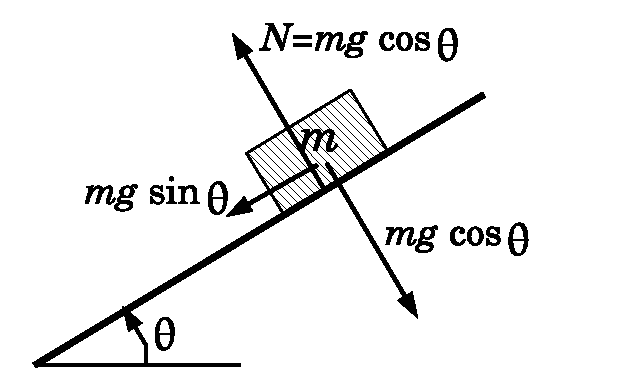
\includegraphics[width=7cm]{slope2.eps}
    \caption{物体は斜面から垂直抗力$N$を受ける。}\label{fig:slope2}

    \centering
    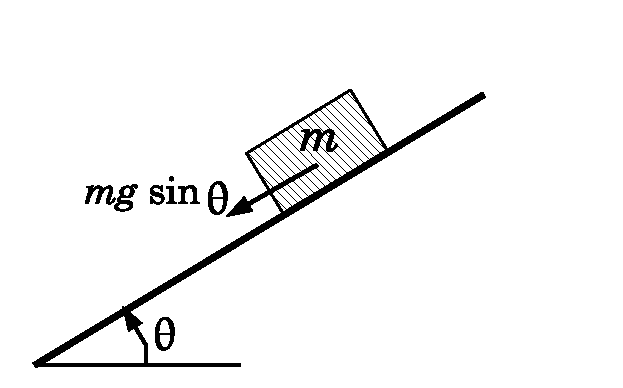
\includegraphics[width=7cm]{slope3.eps}
    \caption{結局, 物体は斜面に平行な力だけを受ける。}\label{fig:slope3}
\end{figure}

このとき, 図\ref{fig:slope}のように, 鉛直下向きの重力$mg$は, 斜面に沿った方向
の力と斜面垂直方向の力に分解して考えてもよい。前者の大きさは$mg\sin\theta$, 
後者の大きさは$mg\cos\theta$である。

と言われても, なぜ, 斜面に沿った方向と斜面垂直方向に分解するのだろうか?
そうするのが便利だからだ。というのも, もし斜面が固ければ, 物体が
動き得るのは斜面に平行な向きだけで, 斜面に垂直な方向には動けない。
従って, 斜面に垂直な方向では, 物体に働く力は釣り合っているはずだ。
それをまずあぶり出せば, 物体にかかる合力は求めやすくなる。

さて話を戻すと, 物体にはもともと重力の斜面垂直成分($mg\cos\theta$)
が働いているから, それと同じ大きさで物体を斜面に垂直に押し返す
垂直抗力$N$があるはずだ(図\ref{fig:slope2})。
一方, 今考えている斜面はなめらかなので, 斜面に沿った方向には斜面は物体に力を
およぼさない(つるつるしている!)。結局, 物体に働く重力と斜面から物体が受ける
垂直抗力を足し合わせると, 物体に働く力として, 図\ref{fig:slope3}のように, 
斜面に沿った重力$mg \sin \theta$だけを考えればよいことになる。

%
\begin{q}\label{q:force_rope2}
図\ref{fig:slope4}のように, 傾斜角30度と60度の2つのなめらかな斜面に, 
それぞれ質量3~kgと質量$m$の物体が載せられ, 滑車を介してロープでつながり, 静止している。
物体と斜面の間の摩擦は無く, 滑車とロープの間にも摩擦は無く, ロープの質量は
無視できるほど軽いとする。$m$を求めよ。ヒント:ロープにかかる張力の大きさ
を$T$とする。まず左の物体が静止する条件から$T$の大きさが求まる。そしてその$T$は, 
右の物体にもかかる。
\begin{figure}[h]
    \centering
    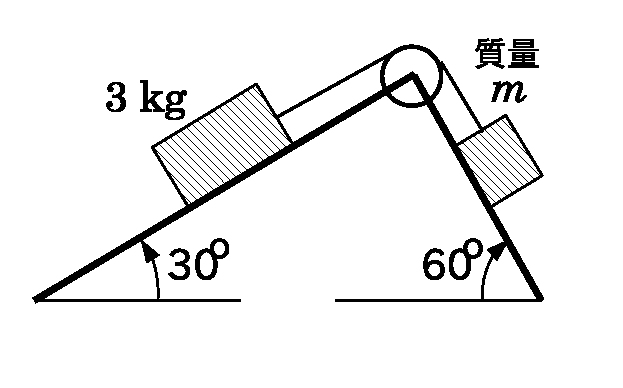
\includegraphics[width=7cm]{slope4.eps}
    \caption{2つの斜面に載せられ, ロープでつながって静止する2つの物体}\label{fig:slope4}
\end{figure}
\end{q}\mv

\begin{faq}{\small\textgt{斜面と滑車の問題は, 高校時代に挫折したとこです。}
... 滑車を介したロープはどこでも張力が同じ, というのがポイントです。}\end{faq}
\hv



\section{摩擦力(クーロンの摩擦法則)}

我々は日常経験から, 物体と物体を接触させたまま動かす(ずらす)
には力が必要だと知っている。ということは, 接触する物体どうしには, それらを
「ずらすまい」とする力が働くのだろう。そのような力を, \textgt{摩擦力}\index{まさつりょく@摩擦力}
という。これは, 以下の2つの式で表現されることが多い。

まず, $N$を, 物体どうしが接触面を介して接触面に対して垂直に互いに押し合う力とする。
2つの物体が相対的に静止している場合(ずれない場合)は, 摩擦力$F_{\text s}$は, 
\begin{eqnarray}
F_{\text s} \leq \mu N\label{eq:friction_s}
\end{eqnarray}
となる。また, 接触面を介して2つの物体が相対的に運動している場合
(ずれる場合)は, 摩擦力$F_{\text m}$は, 
\begin{eqnarray}
F_{\text m}=\mu' N\label{eq:friction_m}
\end{eqnarray}
となる。$F_{\text s}$を\textgt{静止摩擦力}\index{せいしまさつりょく@静止摩擦力}, 
$F_{\text m}$を\textgt{動摩擦力}\index{どうまさつりょく@動摩擦力}という。
また, $\mu, \mu'$は, それぞれ\textgt{静止摩擦係数}\index{せいしまさつけいすう@静止摩擦係数}, 
\textgt{動摩擦係数}\index{どうまさつけいすう@動摩擦係数}
とよばれる定数で, 接触面の物質や状態に依存する。

これを, \textgt{クーロンの摩擦法則}\index{くーろんのまさつほうそく@クーロンの摩擦法則}
という。この「クーロン」は電気的な力の「クーロン力」のクーロンさんと同一人物である。
偉い学者は一人でいくつもの法則を発見するので, 後世の我々は
「クーロンの法則といってもどの法則だ?」と混乱してしまうのだが, まあそれは仕方がない。

さて, 式(\ref{eq:friction_s})に不等号"$\leq$"が入っているのは, 次のような理由
による:摩擦力は, 接触中の2つの物体を「ずらすまい」とする力である。従って, 
静止中の2つの物体の間に, 互いをずらそうとする力がそもそも働いていない場合は, 
あえて「ずらすまい」とする必要はない。そのとき, 静止摩擦力はゼロであるべきだ。
また, たとえ, 「ずらそうとする力」が働いても, それが弱ければ, それを打ち消す
程度の摩擦力があれば十分であり, それ以上は必要ない。
物体が静止しているからには「力のつりあい」が成り立つはずで, となると静止摩擦力は
「ずらそうとする力」と反対の向きに\textgt{同じ大きさで}働いていると考えざるを得ないのだ。
従って, 静止摩擦力は, 
ある一定の範囲($\mu N$以下)で, 「ずらそうとする力」に対応してそれを
"ちょうど"打ち消す力を発揮するのである。

さて, 多くの場合, $\mu'<\mu$である。つまり静止摩擦係数$\mu$は動摩擦係数$\mu'$より
大きい。つまり, 摩擦力は, 静止状態の方が, 動いている状態よりも強い。
それがなぜなのかは, 様々な説があるが, 決定打は無い。

この「クーロンの摩擦法則」も, 一般性の低い「しょぼい」法則である。
単なる経験則であり, この法則から外れるような例もある。摩擦力は, 結局, 
物質と物質の間に働く力なので, おそらく電気力がその根源なのだろう。しかし, 
基本法則からクーロンの摩擦法則を導くことには, まだ誰も成功していない。実は, 
摩擦力の起源や実体は, よくわかっていないのだ。クーロンの摩擦法則は誰もが
「しょぼい」と思っているが, 誰もそれに代わる法則を見つけ出せないでいる...\mv

\begin{faq}{\small\textgt{$\mu' < \mu$となる理由がわかりません。}
... 正確な理由は不明。よく言われるのが, 静止状態では接触面での微妙な凹凸が互いにかみ合って
抵抗が大きいのに対し, 動いているとなかなか凹凸がかみあわず, 滑りやすくなる, という説明。}\end{faq}\mv

\begin{faq}{\small\textgt{「車のブレーキは, タイヤを完全に止めるより, 
少し回しながらのほうが, 地面との摩擦が大きくなって早く止まれる」と
聞いたことがあります。$\mu'<\mu$と関係していますか?}
... まさにそうです。それを利用したのがABS (アンチロック・ブレーキング・システム)です。}\end{faq}\mv


\begin{q}\label{q:friction} 
\begin{enumerate}
\item クーロンの摩擦法則とは何か?
\item 摩擦係数とは何か?
\item 摩擦係数の次元は?
\item アンチロック・ブレーキング・システムを説明せよ。
\end{enumerate}
\end{q}
\mv

\begin{q}\label{q:friction_slope}
傾斜角$\phi$の斜面に, 質量$m$の物体が載って, ぎりぎりで静止している。
これよりも少しでも傾斜がきつければ, 物体は滑り出してしまう。このとき, 傾斜角$\phi$
と静止摩擦係数$\mu$の間に, 次の関係が成り立つことを示せ(このような$\phi$を
\textgt{安息角}という)。
\begin{eqnarray}
\mu=\tan \phi
\end{eqnarray}
\end{q}
\mv

\begin{q}\label{q:slope_spring_friction}
図\ref{fig:slope_spring_friction}のように, 摩擦のある斜面(静止摩擦係数$\mu$)
の上方からバネ(バネ定数$k$)で物体(質量$m$)が吊られて静止している。そのような
状態が実現できるようなバネの伸び縮みの範囲を求めよ。
\begin{figure}[h]
    \centering
    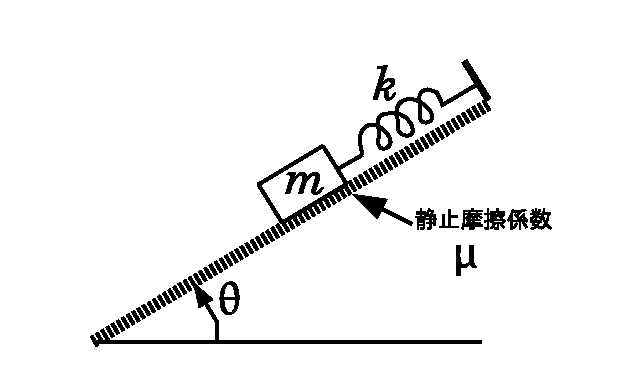
\includegraphics[width=7cm]{slope_spring_friction.eps}
    \caption{摩擦のある斜面に, バネで吊るされた物体}\label{fig:slope_spring_friction}
\end{figure}
\end{q}
\hv


\section{系とは何か?}

これまで扱った多くの例や問題では, それぞれで, 単純化された状況を考えてきた。
例えば図\ref{fig:slope_spring_friction}では, ひとつの斜面と
その上でバネにつながって静止する物体, そしてそれに働く重力\textgt{だけ}を考えた。
実際は世界にはもっとたくさんの物体があるしたくさんの斜面があるしたくさんの力
がある。バネにつながって静止した物体に, 突然上空から隕石が落ちてきて衝突
する可能性も0ではないのだ。

しかし, 科学をやるときは, 世界の中のごく一部だけを
限定的に切り出して単純化し, それ以外のすべてのものを無視した状況を設定する
ことがよくある。そういう状況設定を「\underline{系}」\index{けい@系}
(system)という。それは, 言ってみれば, 当面の問題や議論のためだけ
に極限まで単純化された「世界のモデル」である。例えば, 2つの物体しかない
世界や, バネにつながった物体が斜面に載っている以外には何も無い世界
を考えるのだ。それが系である。

系という言葉は, 本書では今後, たくさん出てくるし, 化学などでもよく出てくるので, 
よく理解しておこう!\mv

\begin{q}\label{q:whatissystem} 系とは何か?\end{q}
\hv




\begin{faq}{\small\textgt{黒板を手で押すとき, 黒板がわずかに
変形してその弾性力が手を押し返すことで手が静止する
と聞きました。でも, 手と黒板の間に, もし作用・反作用の法則がはたらくなら, 黒板は変形
しないでも, 同じ大きさで逆向きの力が手にはたらくと思います。大きさが同じなら釣り合うん
じゃないんですか?}
... とても良い質問です。作用・反作用の法則を学ぶとき, 多くの人が感じる疑問です。
物体が動く(運動状態を変える)かどうかは, 「その物体に働く力」
が釣り合っているかどうかで決まります。ところが作用・反作用
の法則は, 「その物体に働く力」と同じ大きさで逆向きに「相手の物体に働く力」があるという話です。
なので, 「大きさが同じで向きが逆」ということだけを切り出して「ならば力は釣り合うのでは?」
と考えるのは早計です。手が物体を押す力と, 物体が手を押し返す力が「釣り合っている」としても, 
そのことは物体の運動にも手の運動にも, 直接的には無関係なのです。
つまり, 作用・反作用の法則と力のつりあいは無関係なのです。

例として, ボール投げを考えましょう。ボール投げの際, 手はボールに力をかけますが, 
その力はボールを加速することに寄与します(これは後に学ぶ運動方程式で説明
されます)。一方, ボールは等しい大きさで逆向きに手を押し返します(作用・反作用の法則)。
だからボールを投げるときに手は負担を感じるのです(だからピッチャーには体力が必要)。
このとき, ボールにかかる力は釣り合っていません。手にかかる力(ボールから受ける反作用の
力と, 腕の筋肉が手を押す力)も釣り合っていません。

手が黒板を押すとやがて動かなくなるのは, 筋肉(それは肩から手首にかけての部分)
が手(手首から先の部分)を押そうとする力と, 黒板が弾性力(それは結局は垂直抗力)で手
を押そうとする力が釣り合うからです。その弾性力は, 黒板がわずかだけど歪むことで
発生します。従って, 手が黒板を押し始めてから黒板が十分に歪むまでの間は, 黒板の弾性力
は手が押す力よりも弱いので, 黒板は徐々に押し込まれて変形します。その過程では, 
手が押す力の「余り」は, 黒板の変形を加速することに寄与します(運動方程式)。
そして, それらの和, つまり手が押す力と同じ大きさで逆向きの力を手は黒板から
受けます(これが作用・反作用の法則)。これは変形の途中でも, 変形しきったときでも, 
同じこと。ところが変形しきったときは, 黒板の加速度はゼロになるので, 
結局, 手が押す力と黒板の弾性力は等しい大きさになります。}\end{faq}

\begin{faq}{\small\textgt{物体に力がかかるとき, ごくわずかでも
めり込むなら, かなり長い時間, 力をかけていたら, その物体はへこみますか?}
... 力の大きさと素材によりますが, そういう場合も多いでしょう。
短時間では弾性的な(変形に比例した反発力を生じ, 力が取り除かれると
元に戻る)物体も, 長時間, それなりの力にさらされ続けたら, 反発力
を徐々に失い, 変形が戻らなくなったりします。この性質を弾塑性と
呼びます。「レオロジー」という学問分野で扱います。}\end{faq}
\hv

\begin{exq} 質量1~gの物体を1~cm~s$^{-2}$の加速度で動かす力の大きさを1~dynという
(dynはダインと読む)。0.03~Nをdyn単位で書き換えよ。\end{exq}

\begin{exq} 1枚のティッシュペーパーから, 幅2cmほどの帯を2枚切り出し, それぞれ帯Aと帯Bと
呼ぶ。帯Aはそのままにし, 帯Bはねじる(数10回)。それぞれの帯について両端をひっぱって
引きちぎる。どちらが切れにくい(引きちぎるのにより大きな力が必要)か? その理由とともに
述べよ。\end{exq}

\begin{exq} 質量2.0~kgの質点に, 3.0~Nの力をかける。質点に生じる加速度の大きさを求めよ。
ただし基本法則に基づいて根拠もきちんと述べること。\end{exq}

\begin{exq} バネ定数2.0~N/mのバネを, 左端から1.0~N, 右端から1.0~Nの力で
それぞれ引っ張った。伸びはどのくらいか?\end{exq}


%\section{圧力}

%\section{浮力}


\section{解答}

% 自然界に存在する, 根源的な4つの力とは何か?
\noindent{\textbf{答}}\ref{q:4forece} 重力・電磁気力・強い力・弱い力
\mv

% 万有引力定数を$G=6.7 \times 10^{-11}$ N~m $^2$kg$^{-2}$, 地球の半径を$r=6400$ km,
\noindent{\textbf{答}}\ref{q:grav_accel}\\
略。ヒント: \eref{eq:gravity_univ}に適切に値を代入して計算すればよい。ただし, $r$はkmで与えられて
いるので, mに換算すること。つまり, $r=6.4\times10^6$~mとすること。
\vspace{0.2cm}

%\noindent{\textbf{答}}\ref{q:weight_calib} 略。
%\vspace{0.2cm}

% 重力加速度とは何か?
\noindent{\textbf{答}}\ref{q:what_is_g}\\
地表付近にある質量$m$の物体が地球から受ける重力は$mg$
と書ける。このときの定数$g$が重力加速度
\footnote{たまに, 重力加速度とは$GM/r^2$である, という人がいるが, 
間違い。なぜなら, この式は, 地球を静止した完全な球体とみなしており, 
この式に従えば地表のどこでも同じ値になってしまうから。実際の$g$の値は, 
場所によって微妙に異なる。例えば地下に重いものがある場合は, その直上の地表付近では
$g$は大きくなる。低緯度では地球の自転による遠心力(後に学びます)の影響も$g$の
値に入って来る。}。
%また, ウィキペディアなどには「地球表面付近において物体が
%受ける重力の加速度」が重力加速度であると書かれていますが, これもダメです。
%「重力の加速度」とは何か? 重力が加速されるのか? 重力によって何かが加速される
%のか? 地面に置いてある石は重力を受けるけど, 加速されてませんよね?}。
\vspace{0.2cm}

% 高度36000 kmの上空を飛ぶ静止衛星には, 地表での重力の何パーセントの重力がかかるか? 
\noindent{\textbf{答}}\ref{q:geostat_sat}\\
地球中心から地表までの距離を$r_1$, 地球中心から旅客機または静止衛星
までの距離を$r_2$とする。質量$m$の旅客機または衛星が仮に地表にあるときの重力を$F_1$, 
それらが上空にあるときの重力を$F_2$とすると, 
\eref{eq:gravity_univ}より, 
\begin{eqnarray*}
&&F_1=G\frac{Mm}{r_1^2},\quad\quad
F_2=G\frac{Mm}{r_2^2}, \quad\quad\text{従って,}\\
&&\frac{F_2}{F_1}=\frac{r_1^2}{r_2^2}=\Bigl(\frac{6400 \text{km}}{r_2}\Bigr)^2\quad\text{である。}
\end{eqnarray*}
旅客機の場合, $r_2=$6,400~km+10,000~m=6,410~kmを上の式に代入すると, 0.9969$\cdots$。
従って地表での重力の99.7パーセント(ほぼ100パーセント)。静止衛星の場合は, 
$r_2=$(6400~km)+(36000~km)$\fallingdotseq42000$~kmを上の式に代入すると, 0.023$\cdots$。
従って, 地表での重力の約2パーセント。
\mv

% 月の質量は地球の質量の1/80, 月の半径は
\noindent{\textbf{答}}\ref{q:moon_gravity} 地球の半径を$r_1$, 月の半径を$r_2$, 地球の質量を$M_1$, 月の質量を$M_2$とする。
さて, 質量$m$の物体が地表にあるとき地球からうける重力を$F_1$, 月の表面にあるとき月から
うける重力を$F_2$とすると, \eref{eq:gravity_univ}より, 
\begin{eqnarray*}
&&F_1=G\frac{M_1m}{r_1^2},\quad,\quad
F_2=G\frac{M_2m}{r_2^2}\quad\quad\text{従って,}\\
&&\frac{F_2}{F_1}=\frac{M_2}{M_1}\times\Bigl(\frac{r_1}{r_2}\Bigr)^2
\end{eqnarray*}
$M_2/M_1=1/81.3$, $r_2/r_1=1/3.68$を代入すると,
\begin{eqnarray}
\frac{F_2}{F_1}=\frac{1}{81.3}\times3.68^2=\frac{1}{6.00}
\end{eqnarray}
従って, 1/6倍。
\mv

% 地表での平均的な大気圧は, 1000hPa程度であ
%\noindent{\textbf{答}}\ref{q:atm_pressure} 1.0~m$^2$の地表面の上空にある大気の質量を$m$とし, それにかかる重力を$F$とする。
%$F=mg=1000\times10^2$~Pa$\times 1$~m$^2$=$10^5$~N。従って, 
%\begin{eqnarray}
%m=\frac{F}{g}=\frac{10^5\text{ N}}{9.8\text{ m s}^{-2}}\fallingdotseq10^4\text{ kg}
%\end{eqnarray}
%\mv

% クーロンの法則とは何か?
\noindent{\textbf{答}}\ref{q:coulomb_law} 電荷$q_1$と電荷$q_2$をそれぞれ持つ粒子が距離$r$だけ離れて静止して
いれば, その間に, 以下の式であらわされる力$F$が生じる:
\begin{eqnarray*}
F=k\frac{q_1 q_2}{r^2}
\end{eqnarray*}
($k$は定数で, $k=8.987\cdots\times 10^{9}$~N~m$^2$~C$^{-2}$である。)
これを, クーロンの法則と呼ぶ。
\mv

% 電荷素量とは何か?
\noindent{\textbf{答}}\ref{q:element_charge} 電子や陽子が持つ電荷の大きさ(ただし符号を考えない)。$q_e=1.602\times10^{-19}\text{ C}$。
\vspace{0.2cm}

% 互いに1m離れたところに存在する2個の電子の間
\noindent{\textbf{答}}\ref{q:elec_grav_compare}
\begin{enumerate}
\item \eref{eq:coulomb}より, 
\begin{eqnarray}
F_e&=&8.987\times 10^{9}\text{~N~m$^2$~C$^{-2}$}\times\frac{(1.602\times10^{-19}\text{ C})^2}{(1\text{ m})^2}\nonumber\\
   &=&2.3\times10^{-28}\,\, \text{N}
\end{eqnarray}
\item \eref{eq:gravity_univ}より, 
\begin{eqnarray}
F_g&=&6.7 \times 10^{-11}\text{ N m}^2{\text kg}^{-2}
\times\frac{(9.1\times10^{−31}\text{ kg})^2}{(1\text{ m})^2}\nonumber\\
&=&5.5\times10^{-71}\,\, \text{N}
\end{eqnarray}
\item
\begin{eqnarray}
\frac{F_g}{F_e}=2.4\times10^{-43}
\end{eqnarray}
注: このように, クーロン力は重力よりもはるかに大きい。
米国の物理学者リチャード・ファインマンは, 
これを, 「光が陽子1個の端から端まで通り過ぎるのにかかる
時間と, 宇宙の年齢との違いくらい大きい」と表現している。
\end{enumerate}
\vspace{0.2cm}

\noindent{\textbf{答}}\ref{q:Coulomb_EF} その場所に電荷$q$の荷電粒子を
置くと, かかる力の大きさ$F$は, 
\eref{eq:coulomb}より, 
\begin{eqnarray}
F=\frac{k\,q_{\text{e}}\,q}{r^2}
\end{eqnarray}
ここで, $q_{\text{e}}=1.602\times10^{-19}$~C
は電荷素量, $r=1$~m, $k=8.987\times 10^{9}$~N~m$^2$~C$^{-2}$。
電場の大きさは$F/q$だから, 
\begin{eqnarray}
\frac{F}{q}=\frac{k\,q_{\text{e}}\,q}{r^2\,q}=\frac{k\,q_{\text{e}}}{r^2}
\end{eqnarray}
これを計算すると, $1.44\times10^{-9}$~N/C。\mv


% 片端が壁にとりつけられた綱を
\noindent{\textbf{答}}\ref{q:force_rope1}\\
「人対壁」では, 人Aがロープを引く力は, ロープの各箇所で断面の左側に
大きさ$F$で右向きにかかる。その反作用は, 各断面の右側に大きさ$F$で左向きにかかる
(これが張力)。それがロープの左端(壁との接点)まで伝わり, 壁との接点では, 
壁はロープから, 大きさ$F$で右向きの力を受ける。その反作用として, ロープは壁
から大きさ$F$で左向きの力を受ける(この「壁が引く力」がロープの各箇所での
左向きの力の源泉であり, そのおかげで「作用・反作用の法則」とつじつまが合う)。
これは, 壁のかわりに別の人がロープを左端で大きさ$F$の力で左向きにひっぱるのと
同じこと。従って, 「人対人」でも, 「人対壁」でも同じことになる。
\vspace{0.2cm}

%
\noindent{\textbf{答}}\ref{q:force_rope3}\\
君の体には2箇所でロープから上向きにひっぱられている。また, ロープの張力$T$は, 
ロープのどこでも等しい。従って, 君の体には上向きに$2T$の力がかかる。一方, 
重力によって, 君の体に下向きに$mg$の力がかかる。座標軸を, 上向きを正にとると, 力のつりあいから, 
$2T-mg=0$。従って, $T=mg/2$。一方, 君の手がロープを引く力は$T$に等しいので, 
結局, $mg/2$に等しい。
\mv

%
\noindent{\textbf{答}}\ref{q:force_rope4}\\
滑車Bの両端のそれぞれで, ロープの張力$T$が滑車Bを上向きに引く。一方, 
滑車Bには質量$m$の物質にかかる重力$mg$が下向きにかかる。力のつりあい
から, $2T-mg=0$。従って$T=mg/2$。ロープの張力は, ロープのどこでも
等しいから, 君の手にかかる力も$T$, すなわち$mg/2$である。
\vspace{0.2cm}

%
\noindent{\textbf{答}}\ref{q:force_rope5}\\
君の手がロープを引く力は, 君の手の筋肉の筋繊維の収縮から生じる。
この現象は, 筋繊維を構成する高分子の変形によって生じる。分子スケール
の現象を支配する力は, ほとんどの場合, 電気力である。従って, 君の手が
ロープを引く力の根源は電気力である。
\vspace{0.2cm}

%
\noindent{\textbf{答}}\ref{q:Hooke_law}
\begin{enumerate}
\item バネの伸び(変位)$x$と, バネが押す力$F$が比例する, という法則。
\item フックの法則を$F=-kx$と書くときの係数$k$。
\item $k=-F/x$なので, $F$の単位(すなわちN=kg~m~s$^{-2}$)を$x$の
単位(すなわちm)で割ればよい。答は, kg~s$^{-2}$。
\end{enumerate}
\vspace{0.2cm}

\noindent{\textbf{答}}\ref{q:elasticity}\\
力と変位が比例する, という, フックの法則が成り立つような力を
弾性力という。弾性力だけで変形する物体を弾性体という。
\vspace{0.2cm}

\noindent{\textbf{答}}\ref{q:plasticity}\\
塑性体とは, 変形すると元に戻らない物体である。(弾性体は, 
力がかかると変形するが, かかる力が無くなれば元にもどる。)
\vspace{0.2cm}

\noindent{\textbf{答}}\ref{q:spring_moon}\\
質量$m$の物体が地表にあるとき, バネの伸びが$x_0$だったとする。
バネの弾性力と(地球からの)重力のつりあいは次式になる:
\begin{eqnarray}-kx_0+mg=0\end{eqnarray}
一方, 質量$m$の物体が月面にあるとき, バネの伸びが$x_1$だったとする。
月面での(月から受ける)重力は, 問\ref{q:moon_gravity}より, 地表での(地球から受ける)重力の約1/6
なので, バネの弾性力と(月からの)重力のつりあいは次式になる:
\begin{eqnarray}-kx_1+mg/6=0\end{eqnarray}
この2つの式から$mg$を消去すれば, 
\begin{eqnarray}kx_1=kx_0/6\end{eqnarray}
従って, $x_1=x_0/6$。従って, 月面でのバネの伸びは, 地表での約1/6倍。
\vspace{0.2cm}

\noindent{\textbf{答}}\ref{q:spring_double_parallel}\\
下向きに座標系をとる。左側のバネをA, 右側のバネをBと呼ぶ。
バネAについて, バネが下端に働く力を$F$, 伸びを$x$とすると, フックの法則より, 
\begin{eqnarray}F=-kx\end{eqnarray}
である。左右対称なので, まったく同じ式が, バネBについても成り立つ。
一方, 質量$M$の物体にかかる力は, 2つのバネから受ける力, つまり$2F$と, 
重力$Mg$である。物体が静止するには合力はゼロだから, 
\begin{eqnarray}2F+Mg=0\end{eqnarray}
これらの式から$F$を消去すると, 
\begin{eqnarray}-2kx+Mg=0\end{eqnarray}
従って, 
\begin{eqnarray}x=\frac{Mg}{2k}\end{eqnarray}
である。バネが1本だけのときは, $x=Mg/k$なので(\eref{eq:x_mg_k}), この
結果は, $k$が2倍になったとみなせる。
\vspace{0.2cm}

\noindent{\textbf{答}}\ref{q:spring_double_series}\\
下向きに座標系をとる。上のバネをC, 下のバネをDと呼ぶ。
バネCについて, バネが下端に働く力を$F_1$, 伸びを$x_1$とすると, フックの法則より, 
\begin{eqnarray}F_1=-kx_1\end{eqnarray}
である。バネDについても同様に, バネが下端に働く力を$F_2$, 伸びを$x_2$とすると, 
フックの法則より, 
\begin{eqnarray}F_2=-kx_2\end{eqnarray}
である。一方, 質量$M$の物体にかかる力は, バネDが下端に働く力, つまり$F_2$と, 
重力$Mg$である。物体が静止するには合力はゼロだから(力のつりあい), 
\begin{eqnarray}F_2+Mg=0\end{eqnarray}
である。また, バネDにかかる力は, バネCが下端に働く力$F_1$と, 物体がバネDを引っ張る
力(つまり重力)である。バネDに関する力のつりあいから, 
\begin{eqnarray}F_1+Mg=0\end{eqnarray}
これらの式から, 
\begin{eqnarray}Mg=-F_1=-F_2=kx_1=kx_2\end{eqnarray}
従って, 
\begin{eqnarray}x_1=x_2=\frac{Mg}{k}\end{eqnarray}
である。2本のバネの伸びの合計$x$は, 
\begin{eqnarray}x=x_1+x_2=\frac{2Mg}{k}\end{eqnarray}
バネが1本だけのときは, $x=Mg/k$なので(\eref{eq:x_mg_k}), この
結果は, $k$が1/2倍になったとみなせる。
\vspace{0.2cm}

\noindent{\textbf{答}}\ref{q:spring_big}\\
問\ref{q:spring_double_series}と同様に考えれば, バネ定数$k$のバネを$a$本, 縦につなぐと, 
バネ定数は$k/a$となる。問\ref{q:spring_double_parallel}と同様に考えれば, バネ定数$k/a$のバネを$b$本, 
束ねる(並列につなぐ)と, バネ定数は$bk/a$となる。
\vspace{0.2cm}

\noindent{\textbf{答}}\ref{q:YoungModulus}\\
\begin{enumerate}
\item $E=kL/A$で, $k$のSI単位はkg~s$^{-2}$, $L/A$のSI単位はm/m$^{2}$=m$^{-1}$なので, $E$の単位は
kg~s$^{-2}$m$^{-1}$。順番を入れ替えてkg~m$^{-1}$~s$^{-2}$などでもOK。なんと! これはPa, すなわち
圧力のSI単位ではないか!
\item 約$2.0\times10^{11}$~Pa。
\item まずこの鉄線のバネ定数$k$を求める。$L=10$~m, $A=3.14\times(0.002\text{ m}/2)^2=3.1\times10^{-6}$~m$^2$。
従って, $k=EA/L=6.2\times10^{4}$~kg~s$^{-2}$。さて, 質量$m$の物体を吊り下げたときの伸び$x$は, 
\begin{eqnarray*}x=\frac{mg}{k}=\frac{10\text{ kg}\times9.8\text{ m s}^{-2}}{6.2\times10^4\text{ kg s}^{-2}}=1.6\times10^{-3}\text{ m}\end{eqnarray*}
従って, 1.6~mm (約2~mm) 伸びる。
\item 伸びはバネ定数に反比例する。バネ定数は断面積に比例する。従って, 伸びは断面積に反比例
する。従って, 直径を半分にすると断面積が1/4倍になり, 伸びは4倍になる。従って, 伸びは6.4~mmになる。
\item 銅のヤング率は$1.3\times 10^{11}$~Pa。鉄の約0.65倍。伸びはバネ定数に反比例し, バネ定数は
ヤング率に比例する。従って伸びはヤング率に反比例する。従ってヤング率が0.65倍になれば伸びは1/0.65倍。
従って, 2.5~mm程度になる。
\end{enumerate}
\vspace{0.2cm}

%
\noindent{\textbf{答}}\ref{q:stress_strain}
\begin{enumerate}
\item $\sigma=F/A$より, $\sigma$のSI単位は, kg~m~s$^{-2}$/m$^2$ =kg~m$^{-1}$s$^{-2}$=Pa。
\item $\epsilon=x/L$より, $\epsilon$の単位は, m/m=1。従って, 単位無し! (無次元)
\end{enumerate}
\vspace{0.2cm}

% 傾斜角30度と60度の2つのなめらかな斜面に, 
\noindent{\textbf{答}}\ref{q:force_rope2}\\
3~kgの物体にかかる重力の, 斜面平行方向の大きさは, $(3\text{ kg})\times g\times \sin (\pi/6)$。
質量$m$の物体にかかる, 斜面平行方向の力の大きさは, $mg\times \sin (\pi/3)$。これらは
ともにロープの張力と等しい。ロープの張力$T$は, ロープのどこでも等しいから, 
$T=(3\text{ kg}) g \sin (\pi/6)=mg \sin (\pi/3)$。従って, 
\begin{eqnarray}
m=\frac{(3\text{ kg})g\sin(\pi/6)}{g\sin(\pi/3)}=\sqrt{3}\text{ kg}\fallingdotseq 1.7\text{ kg}
\end{eqnarray}
\mv

%
\noindent{\textbf{答}}\ref{q:friction}
\begin{enumerate}
\item 物体どうしが接触している場合, 静止摩擦力$F_{\text s}$と動摩擦力$F_{\text m}$が, 
$F_{\text s} \leq \mu N, F_{\text m}=\mu' N$となること。ここで, $N$は物体どうしが
互いに接触面に垂直に押し合う力。$\mu, \mu'$は, それぞれ静止摩擦係数, 
動摩擦係数とよばれる定数。
\item クーロンの法則が上の式のようにかける時の, $\mu$や$\mu'$のこと。
\item $\mu'=F_{\text m}/N$であり, $F_{\text m}$も$N$も力なので, その比である$\mu'$は無次元。
$\mu$も同様に無次元。
%\item 略。
\end{enumerate}
\mv

\noindent{\textbf{答}}\ref{q:friction_slope}\\
質量$m$の物体に, 斜面に平行にかかる重力(重力の斜面成分)は$mg \sin \phi$。
これが静止摩擦力$F_{\text s}$とつりあっている。いま, 静止摩擦力は上限の状態なので, クーロンの
摩擦の法則より, $F_{\text s}=\mu N$。ここで$N$は物体と斜面の間に働く, 斜面に垂直方向の力で
あり, これは重力の斜面垂直成分に等しい:$N=mg\cos\phi$。従って, $F_{\text s}=\mu mg\cos\phi$。
斜面に平行な方向の力のつりあいより, $mg \sin \phi=F_{\text s}=\mu mg\cos\phi$。従って, 
\begin{eqnarray}\mu=\frac{mg\sin\phi}{mg\cos\phi}=\frac{\sin\phi}{\cos\phi}=\tan\phi\end{eqnarray}
\mv

\noindent{\textbf{答}}\ref{q:slope_spring_friction}\\
斜面に平行で上向き(上り坂方向)に$x$軸をとる。物体をとりつける前のバネの
自然長での末端位置を$x=0$とし, 物体をとりつけた後のバネの末端位置を$x$とする。
物体にかかる, 摩擦力以外の力は, 重力: $-mg\sin\theta$, 弾性力: $-kx$の
2つである。この合力が, 静止摩擦力$F_{\text s}$と釣り合うのだから, 
\begin{eqnarray}-mg\sin\theta-kx+F_{\text s}=0\end{eqnarray}
である。ここで, 垂直抗力は$mg\cos\theta$なので, 
$|F_{\text s}|\leq\mu mg\cos\theta$である。従って, 
\begin{eqnarray}|F_{\text s}|=|mg\sin\theta+kx|\leq\mu mg\cos\theta\end{eqnarray}
である。従って, 
\begin{eqnarray}-\mu mg\cos\theta\leq mg\sin\theta+kx\leq\mu mg\cos\theta\end{eqnarray}
である。従って, 
\begin{eqnarray*}-\mu mg\cos\theta-mg\sin\theta\leq kx\leq\mu mg\cos\theta-mg\sin\theta\end{eqnarray*}
である。従って, 
\begin{eqnarray*}\frac{mg}{k}(-\mu \cos\theta-\sin\theta)\leq x\leq\frac{mg}{k}(\mu \cos\theta-\sin\theta)\end{eqnarray*}\mv

%\noindent{\textbf{答}}\ref{q:whatissystem} 略。

\begin{faq}{\small\textgt{解答を省略するの, やめてください。} ... 
これ, すごく悩ましい話です。私は10年くらいかけて数学や物理学の授業テキストを作っていますが, 最初のころは問題の解答が雑だったり「略」が多かったのです。その頃は, 学生がよく「問題が解けません...」といって質問に来ました。そして問題を一緒に考えて, 単なる「正解」だけでなく, 学生の考え方の癖や, 勉強法などまでも, 助言できました。解答のついていない問題を友達と一緒に考えているうちに, 数学や物理学の楽しさにのめりこんでしまった, というタイプの学生もたくさんいました。

しかし, 学生から「ちゃんと解答をつけてください」と言われて, 丁寧に解答をつけるようにしたら, 学生は質問に来なくなりました。それで学力は伸びたかというと, そうでもありません。むしろ, 「単に正解を覚えて再現してるだけ」で, 深くは理解していない学生が増えました。

学問は, 「誰かが作った正解を覚えこむもの」ではなく, 自分の頭で納得するまで考えるものです。そこが苦しいところでもあり, 楽しいところでもあります。そしてそれは大学教育の最も大事な部分です。「問題の解答」は, そこにおいて, むしろ悪影響をもたらすものではないか, と, 私は悩んでいます。あなたはどう思いますか?}\end{faq}

\begin{faq}{\small\textgt{でも, 自力で解いた後の答え合わせには, 正解を教えてもらうことが必要です。} ... 
大学では「正解」は, 誰かが与えるものでなく, あなたが作るものです。いろんな観点から考えぬいて, 「これが正しい!」とあなた自身が納得し, 人にも説明できるなら, それが「正解」です。実際, 教員や教科書が与える「正解」には, 間違っていることも多いのですよ。お互いの「正解」を比べて議論しながら, 「より正しい正解」を作るのです。学問とは本来, そういうものです。}\end{faq}

\begin{faq}{\small\textgt{でも, 解答が無いと勉強の効率が悪いです。いくら考えてもわからないときは解答を見るしかありません} ... 
その気持ちわかります。私もそう思います。でもね。解答があると, 突き詰めて考える前にどうしても見たくなってしまうものです。あなたはそれを自制できるかもしれませんが, 「問題は正解を丸写しにして覚えるもの」と思っている人も多いのです。}\end{faq}

\begin{faq}{\small\textgt{じゃあ, どうすればいいのですか?} ... 
質問に来ればよいのです。あるいは, 友達同士で一緒に考えたり教え合えばよいのです。}\end{faq}


\chapter{仕事とエネルギー}

{\small 注: この章を理解するには, 数学リメディアル教材で「積分」を理解していることが必要。}

本章では「エネルギー」について学ぶ。世の中には「エネルギー」という言葉が溢れているが, 
なぜそんなに「エネルギー」って大事なのだろうか? ていうか, そもそも「エネルギー」って
何なのだろうか? それを理解するには, まず「仕事」という概念を定義しなければならない。
そこから話をはじめよう。\\

\section{仮想仕事の原理}

前章で, 体を滑車に吊るす話や, 動滑車で物を持ち上げる話や, 質量の異なる物体を
2つの斜面に置いてロープでつないで静止させる話などを学んで, 君は不思議に
思わなかっただろうか? これらの話は, とりあえず力のつりあいや, 作用・反作用
の法則などは, 満足させている。だが, 物体をその重さの半分の力で
持ち上げられる, というのは不思議だ。我々の日常感覚では, ある物を持ち
上げるにはその重さと同じ力が必要では? と, シンプルに考えてしまう。
しかし実際の自然はそうではない。不思議だ。気持ち悪い。この不思議さ
をうまく説明し, この気持ち悪さから我々を救ってくれるシンプルな法則
は無いのだろうか? 

それが, ここで学ぶ「仮想仕事の原理」だ。これは「力のつりあい」
を, もっと普遍的に述べた物理法則である。「力のつりあい」と等価だが, ある意味, それ
よりも深く, 根源的なものを内包した法則だ。

\begin{exmpl}
動滑車で物を持ち上げる話(問\ref{q:force_rope4})では, 滑車やロープや天井などが
互いに及ぼす力(張力など)は別とすれば, 関与する力は, 君がロープを下向きに引く力$T$と, 物体に
下向きにかかる重力$mg$だ。ここで, 仮想的に, 君がロープを, ちょっとだけ引っぱった
としよう(図\ref{fig:string4vw})。このとき, 滑車Bが$\Delta x$だけ持ち上がったとする。
すると, 当然, 物体も同じだけ, つまり$\Delta x$だけ持ち上がる。このとき, ロープの動きを
たどって考えれば, 君がロープを引っ張った長さは$2\Delta x$であることがわかるだろう
\footnote{滑車Bの左右端からそれぞれ長さ$\Delta x$だけ上の部分が, 
引っ張った後には無くなっている。これらの長さの合計は(左右にそれぞれ1つずつあるので)
$2\Delta x$である。}。
\begin{figure}[h]
    \centering
    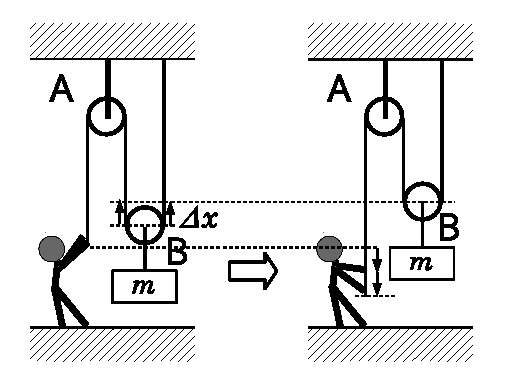
\includegraphics[width=8cm]{string4vw.eps}
    \caption{動滑車を使う持ち上げ。物体を$\Delta x$だけ上昇させるには
ロープを$2\Delta x$だけひっぱる必要がある。}\label{fig:string4vw}
\end{figure}

このとき, 下向きに座標をとり, それぞれの力と, その力が働く点が動いた距離の
掛け算を考え, それを合計してみる。
\begin{eqnarray}
T(2\Delta x) + mg (-\Delta x)
\end{eqnarray}
ここで, 第二項の$(-\Delta x)$のマイナスは, 座標の向き(下向き)とは
逆の上向きに物体が移動することをあらわす。で, \underline{\textgt{だまされたと思って, 
これを0とおいてみよう}}:
\begin{eqnarray}
2T\Delta x - mg \Delta x=0
\end{eqnarray}
すると, 
\begin{eqnarray}
T=\frac{mg}{2}
\end{eqnarray}
という, 正しい答えが得られる。これが仮想仕事の原理の例である。(例おわり)
\end{exmpl}

仮想仕事の原理とは以下のようなものである:
\begin{itembox}{仮想仕事の原理}\index{かそうしごとのげんり@仮想仕事の原理}
力がつりあっている系では, 仮想的な微小変位に伴って外力のなす仕事の総和は0である。
\end{itembox}

「仮想的な微小変位」とは, 上の例で言えば, 君がロープを引く
$2\Delta x$や, 物体が上に上がる$\Delta x$のことだ。
「外力」とは, 君が引く力と, 物体にかかる重力のことだ。
そして, 
\begin{itembox}{仕事の定義}\index{しごと@仕事}
「力と, その力が働く点が"力と同じ向き"に動いた距離との掛け算」を「\underline{仕事} (work)」という。
\end{itembox}

なんで「仕事」とか「仮想的な微小変位」とかの得体の知れぬものを持ち出してこんな
「原理」を考えるのだろうか? それは, こうすればうまく(シンプルに無矛盾に)
いろんな物事を説明できるからだ。なぜこんな原理が成り立つのか, その
理由は誰も知らない。自然はそうなっているのだ。

この例では, 確かに動滑車のおかげで, ロープを引っ張る力は半分になったが, 
そのかわり, ひっぱる長さは倍になってしまった。つまり, 同じ高さだけ持ち上げ
ようとすると, かかる力が半分なら, ひっぱる長さ(距離)を倍にしなければならない。
つまり, たとえ必要な力は動滑車などで変えることができても, 力と距離の掛け算, 
つまり仕事は, 変えることができない。それが自然の摂理なのだ。だから, 
仕事という概念が便利なのだ。

もうひとつの例を考えよう。前章で考えた, 2つの斜面に物体を置いてロープで
つないで静止させる話である。
\begin{figure}[h]
    \centering
    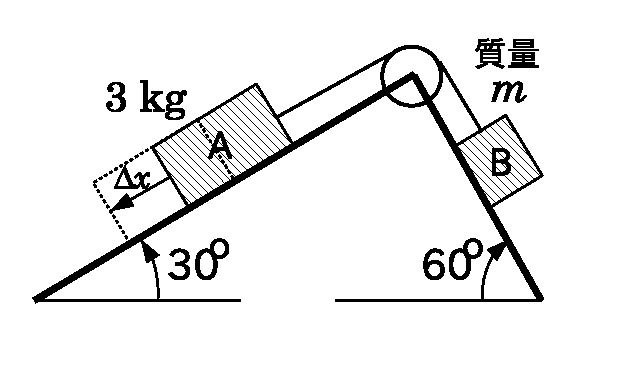
\includegraphics[width=7cm]{slope4b.eps}
    \caption{2つの斜面に載せられ, ロープでつながって静止する2つの物体。図\ref{fig:slope4}改変。}\label{fig:slope4b}
\end{figure}
\begin{exmpl}
前章の問\ref{q:force_rope2}において, 物体Aを斜面に沿って
左下向きに$\Delta x$だけ動かしてみよう(図\ref{fig:slope4b})。すると, ロープにつながっている物体Bも, 
斜面に沿って左上向きに$\Delta x$だけ動くはずだ。このとき, 
物体Aに関して重力がなす仕事は, (3~kg)$g\{\sin(\pi/6)\}\Delta x$である。一方, 
物体Bに関して重力がなす仕事は, $-mg\{\sin(\pi/3)\}\Delta x$である。マイナスがつくのは, 物体Bが重力
と逆方向(上方向)に移動したからだ。仮想仕事の原理より, 
\begin{eqnarray}
\Bigl(3\text{ kg})g\Bigl(\sin\frac{\pi}{6}\Bigr)\Delta x-mg\Bigl(\sin\frac{\pi}{3}\Bigr)\Delta x=0
\end{eqnarray}
ここから, $m=\sqrt{3}$~kgが出てくる。(例おわり)
\end{exmpl}

%
\begin{q}\label{q:def_work} 
\begin{enumerate}
\item 仕事とは何か?
\item 仕事の単位をSI基本単位による組み立て単位で表せ。それをJ(ジュール)と呼ぶ。
\item 仮想仕事の原理とは何か? 
\end{enumerate}
\end{q}
\mv

%
\begin{q}\label{q:teko}
君は「てこの原理」\index{てこのげんり@てこの原理}を聞いたことがあるだろう。これは仮想仕事の
原理から導くことができる。図\ref{fig:balance}上のように, 支点Sの上に, 
左右に長さ$l_1$, $l_2$を持つ「てこ」が置かれ, 左右それぞれの端にぞれぞれ質量
$m_1$, $m_2$の物体1, 2が載っている。これを, 図\ref{fig:balance}下のように, 
左側が下がるように, 仮想的に小さな角$\theta$だけ下げる。このとき, 
\begin{enumerate}
\item 左端がもとの状態から$h_1$だけ下がり, 右端がもとの状態より$h_2$だけ上がるとすると, 
\begin{eqnarray}
h_1&=&l_1\sin\theta \\
h_2&=&l_2\sin\theta
\end{eqnarray}
となることを示せ。
\item 物体1における重力による仮想仕事は$m_1gl_1\sin\theta$, 
物体2における重力による仮想仕事は$-m_2gl_2\sin\theta$となることを
示せ。 
\item 仮想仕事の原理より, 次式(てこの原理)を導け:
\begin{eqnarray}
m_1l_1=m_2l_2\label{eq:principle_balance}
\end{eqnarray}
\end{enumerate}
\end{q}
\begin{figure}[h]
    \centering
    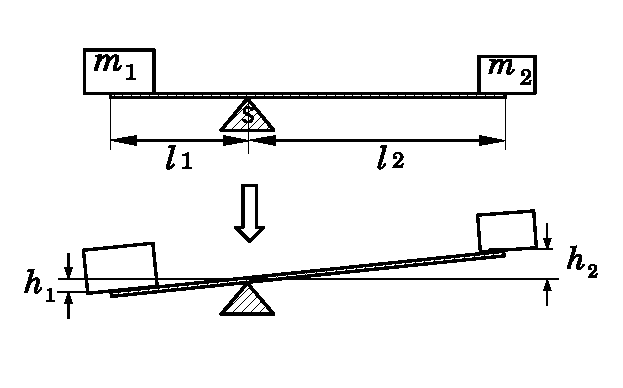
\includegraphics[width=7cm]{balance.eps}
    \caption{仮想仕事の原理からてこの原理を導く。}\label{fig:balance}
\end{figure}

前章で述べたように, 物体が静止しているとき, 「力のつりあい」が実現している。
しかし, 実は, 「大きさを持つ物体」についてはそれに加えて, 上述の「てこの原理」
に相当する, 「モーメントのつりあい」\index{もーめんとのつりあい@モーメントのつりあい}
というものも実現する。モーメントとは, 簡略に言えば, ある点(支点)からの距離と, 
それに直交する力との積だ。そして, モーメントのつりあいとは, モーメントの
合計が0になるということだ。高校物理を学んだ人は聞いたことがあるだろう。
しかし, これをきちんと正しく記述し, 理解するには, 数学で「ベクトルの外積」
というのを学ばねばならないので, 今は詳述しない(後の章で学ぶ)。ただし, 
ここでは, 「仮想仕事の原理は, 力のつりあいだけでなく, モーメントのつりあいまでも
含んだ, 一般性の高い法則だ」ということを認識しておこう。\mv

\begin{q}\label{q:jack}
図\ref{fig:jack}のようなジャッキについて, 半径$r$のハンドルを1回転すると, 
上載物は$\Delta y$だけ持ちあがるとする。摩擦は無視する。
\begin{enumerate}
\item ハンドルをまわすのに必要な力を$F$とする。ハンドルを1回転するときに, 君の手がなす仕事は
\begin{eqnarray}2\pi r F\end{eqnarray}
であることを示せ。
\item 上載物の質量を$m$とする。ハンドルを1回転するときに, 重力のなす仕事は
\begin{eqnarray}-mg\Delta y\end{eqnarray}
であることを示せ。
\item 次式を示せ:
\begin{eqnarray}2\pi r F-mg\Delta y=0\end{eqnarray}
\item 次式を示せ:
\begin{eqnarray}F=\frac{mg\Delta y}{2\pi r}\end{eqnarray}
\item $m=1000$~kg, $r=0.2$~m, $\Delta y=0.003$~mのとき, $F$はどのくらいか?
\end{enumerate}
\begin{figure}[h]
    \centering
    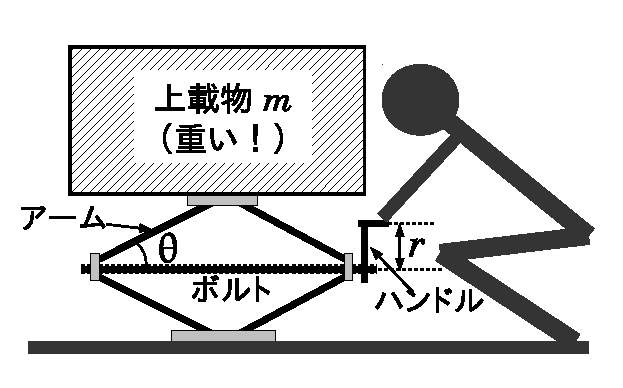
\includegraphics[width=6cm]{jack.eps}
    \caption{ジャッキで物を持ち上げる。}\label{fig:jack}
\end{figure}
\end{q}

\begin{faq}{\small\textgt{仮想仕事の原理の「仮想的な微小変位」
はどうして仮想的である必要があるんですか?}
... 「微小変位」という考え方自体がそもそも仮想的です。バランスしている系に
少しでも変化を加えたら, バランスが崩れるかもしれない。でも, 「バランスを崩さない程度に
小さな変位」というのが微小変位であって, そもそもそんなの厳密には
現実的に無理じゃね?という気持ちがあるから「仮想」なのです。}\end{faq}\mv

\begin{faq}{\small\textgt{仮想仕事の原理に鳥肌が立ちました。
自然の不思議さを感じざるを得ません。}
... このような原理を見つける旅が, 学問としての物理学なのでしょう。}\end{faq}
\hv



\section{仕事とエネルギー}

さて, 仮想仕事の原理では, 「仕事」という量が重要な働きをした。それにとどまらず, 
仕事は, 物理学の全般にわたって, 重要な役割を果たす概念だ。例として, 
図\ref{fig:string4vw}の例をもういちど考えよう。君がロープを引くことで
\begin{eqnarray*}2T\Delta x\end{eqnarray*}
という仕事をしたとき, 同時に, 質量$m$の物体にかかる重力が
\begin{eqnarray}-mg\Delta x\end{eqnarray}
という仕事をした。このとき, 仮想仕事の原理から, 両者の和は0である。

君がロープを引くことによって君は仕事をし, 実際, 疲れる。しかしその努力は, 
重力に逆らって物体が上昇した, という結果(重力による負の仕事)に残っている。
この上昇した状態で物体に別のロープとか滑車とかてこをつければ, 今度は物体が
下がることによって, また別の物体を持ち上げることができるだろう。

このような話は, お金のやりとりに似ていないだろうか? A君がB君に1000円を譲渡したとする。
なぜそんなやりとりが起きたか, とか, それによって2人の関係はどうなるか, という興味も
あるが, 2人以外の人にしてみれば, お金のやりとりは2人の間で完結している(2人あわせた
収支は0である)。そして, A君からもらった1000円で, こんどはB君がCさんから
何かを買うことができる。

物理学における仕事とは, この話の「お金」のような役割をする。A君, B君, Cさん, ...
とお金が手渡されていくように, 君がロープを引くことでなした仕事は, 後々まで, 形を変えながら, 
様々なところに受け渡されるのだ。そのように, 仕事を普遍化した
量を, 物理学では\underline{エネルギー}\index{えねるぎー@エネルギー}という。
\textgt{エネルギーとは, 仕事が形を変えた量, もしくは仕事に形を変えることができる量である}。
エネルギーは仕事と同じ次元を持ち, その単位は, SI単位系ではJである。

\begin{q}\label{q:energy}
エネルギーとは何か? 
\end{q}

エネルギーには, 様々な形態がある。熱もエネルギーだ。
なぜか? 例えば気体に熱を加えると膨張し, まわりのものを移動
させることができる。つまり, 仕事ができる。だから熱はエネルギーである。

光もエネルギーの一形態だ。なぜか? 太陽光を浴びると暖かくなる, 
つまり熱を受け取ることができる。熱はエネルギーなので, 光はエネルギー
を運ぶのだ。

熱は, 後に学ぶ「運動エネルギー」というタイプのエネルギーに
帰着させて考えることができる。また, この章の後半で学ぶ
「ポテンシャルエネルギー」というタイプのエネルギーもある。
物質が化学反応するときに出る熱や光は, 物質の分子レベルでの
ポテンシャルエネルギーの変化によるものである。\mv

さて, 仕事について, もう少し, 丁寧に数学的に意味づけよう。

さきほど, 仕事とは, 「力と, その力が働く点が"力と同じ向き"に動いた距離との掛け算」である
と述べたが, それが成立するのは, その点の移動中に, 力がほとんど変化しないことが
必要である(でなければ, どの時点での力を掛け算すればいいのかわからない)。では, 
移動中に力が次第に変化するような場合は, 仕事はどのように定義されるのだろうか? 

%2011.4.2 ヤマサキ 仕事の定義を定式化する中の, シグマをインテグラルにするところ。今のリメディアルの記述と整合的にするために式を追加。
いま, ある物体に力$F$がかかっているとき, それを力の向きに$\Delta x$だけ
動かす。 $\Delta x$だけ動かす間には$F$は変化しないと考える。すると, その力がする仕事$\Delta W$は, 
\begin{eqnarray}
\Delta W=F\Delta x \label{eq:work}
\end{eqnarray}
である。これは仕事の定義だ。これをたくさん繰り返すことを考えよう。
いま, 座標上で, 位置$x_0$にある物体を, 位置$x_1$まで運ぶとする。
この間, 物体にかかる力は変化するかもしれないが, $x_0$から$x_1$
まではとても近くて, その間の力の変化は無視できるくらいに小さいと
する(逆に言えば, 力の変化が無視できるくらいに, $x_0$と$x_1$を
近づける)。つまり, この間の力は$F_1$でほぼ一定値とみなせる。このときの
仕事$\Delta W_1$は, 上の式から, 
\begin{eqnarray}\Delta W_1\fallingdotseq F_1\Delta x_1\end{eqnarray}
である($\Delta x_1=x_1-x_0$とする)。位置$x_1$まで来た物体は, 
こんどは$x_1$のすぐ近くの位置$x_2$まで運ばれ, その間, 物体にかかる力は$F_2$で一定で
あるとする(ただし$F_2$は$F_1$と同じとは限らない)。このとき
の仕事$\Delta W_2$は, 同様に, 
\begin{eqnarray}\Delta W_2\fallingdotseq F_2\Delta x_2\end{eqnarray}
である($\Delta x_2=x_2-x_1$とする)。以下同様に, 物体
をすこしずつ$x_3, x_4, \cdots, x_n$まで順次運び($n$は正の整数), 各
ステップでは物体に$F_3, F_4, \cdots, F_n$というそれぞれ一定値の
力がかかっていると, 各ステップでの仕事は, 
\begin{eqnarray}
\Delta W_3\fallingdotseq F_3\Delta x_3\nonumber\\
\Delta W_4\fallingdotseq F_4\Delta x_4\nonumber\\
\cdots\nonumber\\
\Delta W_n\fallingdotseq F_n\Delta x_n\label{eq:W_nF_nDx_n}
\end{eqnarray}
となる。これらを辺々で合計すれば, 
\begin{eqnarray}\sum_{k=1}^{n}\Delta W_k\fallingdotseq \sum_{k=1}^{n}F_k\Delta x_k\end{eqnarray}
となる。左辺は, 物体を$x_0$から$x_n$まで運ぶときの全体の仕事であり, これを
$W$と書こう:
\begin{eqnarray}
W\fallingdotseq \sum_{k=1}^{n}\Delta W_k\fallingdotseq\sum_{k=1}^{n}F_k\Delta x_k \label{eq:one_step_before_work2}
\end{eqnarray}
ここで$n$を十分大きくとって, $x_1, x_2, ..., x_n$の分割を十分に細かく
すれば, すなわち, \eref{eq:one_step_before_work2}の極限として, 
\begin{eqnarray}
W=\lim_{\substack{n\rightarrow \infty\\\Delta x_k\rightarrow 0}}\sum_{k=1}^{n}F_k\Delta x_k
\end{eqnarray}
を考えれば, 「数学リメディアル教材」の積分の定義より, 次式が成り立つ:
\begin{itembox}{仕事の定義(力が一定でない場合)}
物体を位置$a$から位置$b$まで運ぶときの仕事は, 
\begin{eqnarray}
W=\int_{a}^{b} F(x)\,dx \label{eq:work2}
\end{eqnarray}
\end{itembox}
ここで$x_0$を$a$に, $x_n$を$b$に, 改めて書き換えた。$F(x)$は$x$の各点で物体が受ける力
だ。この式(\ref{eq:work2})は, 仕事の定義式(\ref{eq:work})を, 「力が次第に
変化する場合」に拡張した(つまり, より一般性の高い)仕事の定義式である。\mv

\begin{exmpl}\label{ex:work_fall}
 質量$m$の物体が, 地表付近で$mg$という大きさの重力を受けて, 高さ$h_0$から$h_1$まで
変化する。重力のなす仕事を求めよう。座標軸を上向きにとると, 重力は, 式(\ref{eq:gravity_earth})より, 
\begin{eqnarray}F=-mg\end{eqnarray}
である。ここで右辺のマイナスは, 重力が座標軸の向きとは逆向きであることを表す
\footnote{式(\ref{eq:gravity_earth})では力の向きを考えず, 力の大きさだけを考えていたことに注意せよ。}。
従って, 式(\ref{eq:work2})より, 
\begin{eqnarray}
W&=&\int_{h_0}^{h_1} (-mg)\,dx\nonumber\\
 &=&-mg(h_1-h_0)=mg(h_0-h_1)
\end{eqnarray}
となる。もし$h_0>h_1$なら(つまり物体が下がるとき), $W>0$である。
もし$h_0<h_1$なら(つまり物体が上がるとき), $W<0$である。つまり, 重力に
逆らって動く場合は, 重力のする仕事はマイナスである, ということになる。(例おわり)
\end{exmpl}

\begin{faq}{\small\textgt{例\ref{ex:work_fall}で, 座標軸は下向きじゃダメですか?}
... いいですよ。その場合, $F=mg$となり, $W=mg(h_1-h_0)$。これは本文の結果とは符号が
逆のように見えますが, 今の場合は$h$が大きいと低いので, 結局, 物体が下がると$h_0<h_1$となり, 
そのとき$W$は正になる。 という結論は変わりません。本文で座標を上向きにとったのは, 
「高いところほど$h$が大きい」ほうが, 我々の空間認識では直感に素直だからです。}\end{faq}
\mv

\begin{exmpl}
質量$m$の物体Aが, 質量$M$の物体Bから万有引力を受けながら, 物体Bからの
距離が$R_0$から$R_1$まで変化する。このとき万有引力のなす仕事を求めよう。座標軸を
物体Bから物体Aの向きにとると, 万有引力は, 式(\ref{eq:gravity_univ})より, 
\begin{eqnarray}F=-\frac{GMm}{x^2}\end{eqnarray}
である。ここで右辺のマイナスは, 万有引力が座標軸の向きとは逆向きであることを表す
\footnote{式(\ref{eq:gravity_univ})では力の向きを考えず, 力の大きさだけ
を考えていたことに注意せよ。}。式(\ref{eq:work2})より, 
\begin{eqnarray}
W&=&\int_{R_0}^{R_1} \Bigl(-\frac{GMm}{x^2}\Bigr)\,dx=\Bigl[\frac{GMm}{x}\Bigr]_{R_0}^{R_1}\nonumber\\
 &=&GMm\Bigl(\frac{1}{R_1}-\frac{1}{R_0}\Bigr)\label{eq:work_gravity}
\end{eqnarray}
となる。(例おわり)
\end{exmpl}
\mv

%
\begin{q}\label{q:spring_work}
バネ定数$k$のバネについた物体を, バネの自然状態を原点として位置$x_0$
から位置$x_1$まで動かすときに, バネの弾性力がなす仕事$W$は, 
\begin{eqnarray}
W=-\frac{1}{2}\,k\,(x_1^2-x_0^2)\label{eq:spring_work}
\end{eqnarray}
となることを示せ。ヒント: 式(\ref{eq:Hooke})より$F=-kx$とし, 式(\ref{eq:work2})を使う。
\end{q}
\vspace{0.2cm}

%
\begin{q}\label{q:gas_work}
気体を膨張させたり圧縮したりするときの仕事を考えよう。ある気体が, 断面積$A$の
シリンダー(筒状の容器)に入っており, 上面がピストンで蓋してある。
鉛直上向きに$x$軸をとり, シリンダーの底面で$x=0$とする。ピストンは$x$軸にそって上下に
動くことができる。最初, ピストン(つまり蓋)は$x=h$にあって静止しているとする
(図\ref{fig:gas_piston})。
ピストンは十分に軽いとし, 重力を無視する。気体の圧力を$P$とする。
\begin{figure}[h]
    \centering
    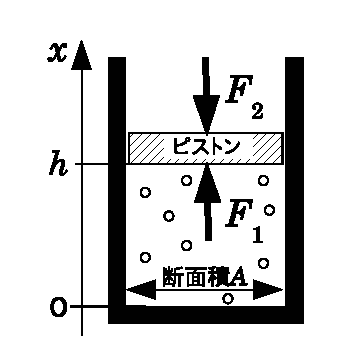
\includegraphics[width=7cm]{gas_piston.eps}
    \caption{気体の入ったシリンダー。}\label{fig:gas_piston}
\end{figure}
\begin{enumerate}
\item 気体の体積$V$は, $V=Ah$と表せることを示せ。
\item 気体がピストンに及ぼす力$F_1$は, 
\begin{eqnarray}F_1=PA\label{eq:gas_work1}\end{eqnarray}
となることを示せ。
\item 外部からピストンにかかる力(それを外力という\footnote{この外力が
具体的に何によるものかは, ケースバイケースであり, ある場合は誰かが手で押さえ
込んでいるのかもしれないし, ある場合はシリンダー外部に充満する気体
の圧力によるものかもしれない。この問題ではその詳細は気にしない。})
を$F_2$とすると, 
\begin{eqnarray}F_2=-PA\label{eq:gas_work2}\end{eqnarray}
となることを示せ。
\item 次に, ピストンをゆっくり動かして, $x=h+dh$の位置に移動させることを考えよう。
$dh>0$なら, 気体は膨張し, $dh<0$なら気体は圧縮される。$dh$は微小であり, 
ピストンが$x=h$から$x=h+dh$まで動く間に$F_1$や$F_2$はほとんど一定である
とみなす。このとき, 外力がなす仕事$dW$は, 
\begin{eqnarray}dW=F_2\,dh=-PA\,dh\label{eq:gas_work3}\end{eqnarray}
となることを示せ。
\item 体積の変化を$dV$とする。すなわち, ピストンの移動後に気体の体積は
$V+dV$になったとする。次式を示せ:
\begin{eqnarray}dV=A\,dh\label{eq:gas_work4}\end{eqnarray}
\item \eref{eq:gas_work3}, \eref{eq:gas_work4}より次式を示せ:
\begin{eqnarray}dW=-P\,dV\label{eq:gas_work5}\end{eqnarray}
\item ピストンを大きく動かし, 体積が$V_1$から$V_2$になるまで変化させることを考えよう。
この間に外力がなす仕事$W$は次式のようになることを示せ:
\begin{eqnarray}
W=-\int_{V_1}^{V_2}P\,dV
\end{eqnarray}
\item ここで, 気体は理想気体であるとしよう。つまり, 理想気体の状態方程式:
\begin{eqnarray}PV=nRT\end{eqnarray}
が成り立つとする($n$はモル数, $R$は気体定数, $T$は絶対温度)。次式が成り立つことを示せ:
\begin{eqnarray}
W=-\int_{V_1}^{V_2}\frac{nRT}{V}\,dV
\end{eqnarray}
\item ここでさらに, ピストンの移動は十分にゆっくりであり, その過程では温度$T$は
一定であるとすると, 次式が成り立つことを示せ:
\begin{eqnarray}
W=nRT\ln\frac{V_1}{V_2}
\end{eqnarray}
\item 1モルの理想気体を摂氏0度(一定)で体積を半分まで圧縮するときに外力がなす仕事を求めよ。
\end{enumerate}
\end{q}
\vspace{0.2cm}

\eref{eq:gas_work5}は, 化学や熱力学で, 非常によく出てくる式だ。ここでは外力が
なす仕事を考えたが, 気体(の圧力)がなす仕事を考えると, それは外力がなす仕事の符号を
逆にしたものである(なぜなら気体がピストンにおよぼす力は外力がピストンにおよぼす
力の逆だから)。それを$dW'$とすると, $dW'=-dW$なので, 
\begin{eqnarray}
dW'=P\,dV
\end{eqnarray}
となる。この式もよく使われるので, \eref{eq:gas_work5}との違いをよく理解して
おこう\footnote{化学や熱力学では, 教科書によって, 外力のなす仕事を$dW$とするものと, 
気体がなす仕事(すなわちここで$dW'$とあらわしたもの)を$dW$とするものがあるので, 
気をつけよう。}。
\hv


\section{ポテンシャルエネルギー}\index{ぽてんしゃるえねるぎー@ポテンシャルエネルギー}

さて, \eref{eq:work2}をみると, 仕事$W$は, 始点$a$と終点$b$の関数だ。特に, 始点$a$
をどこかに固定して(それを基準点と呼ぼう), $W$を$b$だけの関数とみなし, 改めて$b$を$x$と
書けば, $W$は$x$の関数$W(x)$だ。その意味は, 「基準点から位置$x$まで物体を
運ぶときの仕事」である。この$W(x)$の符号を変えたものを\underline{ポテンシャルエネルギー}
\footnote{「位置エネルギー」とか, 単に「ポテンシャル」と言うこともある。}という。すなわち, 
\begin{itembox}{ポテンシャルエネルギーの定義(1)}
\begin{eqnarray}
U(x)=-W(x)\label{eq:potential}
\end{eqnarray}
で定義される関数$U(x)$を, 「\textgt{ポテンシャルエネルギー}」という。
ここで$W(x)$は, 物体を基準点から位置$x$まで運ぶときに, 物体にかかっている力がなす仕事である。
\end{itembox}

\begin{exmpl}\label{ex:gravity_potential_mgh}
上の例\ref{ex:work_fall}で, 地面を基準点とすれば, $h_0=0$となり, $h_1$を
改めて$h$とおけば, $W(h)=-mgh$である。このとき, ポテンシャルエネルギーは, 
\eref{eq:potential}から, 
\begin{eqnarray}
U(h)=mgh\label{eq:potential_g}
\end{eqnarray}
である。(例おわり)
\end{exmpl}

つまり, 物体を高く持ち上げるほど, 重力によるポテンシャルエネルギーは, 
大きくなる。で, 持ち上げられた物体は, てこや滑車を使えば, 別の物体を持ち上げる「仕事」を
することができる。つまり, ポテンシャルエネルギーとは, 力を受けている物体が, ある位置に
あることによって持つエネルギー, つまり位置に付随するエネルギーである。


%
\begin{q}\label{q:def_potential}
ポテンシャルエネルギーとは何か? 
\end{q}

ところで, \eref{eq:potential}の右辺の$W(x)$は, 物体にかかっている力
がなす仕事だ。例えば例\ref{ex:gravity_potential_mgh}では, 重力がなす仕事がそれに相当する。
ところが, 現実的には, 重力がかかっている物体が, ひとりでに重力に逆らって上に移動したりは
しない。誰かが重力に逆らう力をかけて, その物体を持ち上げねば, 物体は上に移動しない。
そのような「誰かの力」がなす仕事$W'(x)$を考えると\footnote{ここで$W'(x)$のダッシュ
は「微分」という意味ではない。単に$W(x)$と区別するための印である。}, それは重力
のなす仕事とは同じ大きさでありながら符号が逆である(力の向きが逆だから)。
すなわち, $W'(x)=-W(x)$だ。それを使うと, ポテンシャルエネルギーは以下のように
定義することもできる:

\begin{itembox}{ポテンシャルエネルギーの定義(2)}
\begin{eqnarray}
U(x)=W'(x)\label{eq:potential2}
\end{eqnarray}
で定義される関数$U(x)$を, 「\textgt{ポテンシャルエネルギー}」という。
ここで$W'(x)$は, 物体を基準点から位置$x$まで運ぶときに, かかっている力に逆らって
誰かがなす仕事である。
\end{itembox}

例\ref{ex:gravity_potential_mgh}では, 物体を地面から高さ$h$まで君が持ち上げる
とすれば, 君は物体に上向きに$mg$という大きさの力をかけ, 上向きに$h$だけ移動
させねばならないので, そのとき君がなす仕事は$W'(h)=mgh$だ。従って
ポテンシャルエネルギーは, \eref{eq:potential2}から, $U(h)=mgh$となり, 
それは\eref{eq:potential_g}に一致する(つじつまが合っている)。

\eref{eq:potential}と\eref{eq:potential2}は, 互いに等価であり, どちらの
定義を採用してもかまわない。これらの2つの定義は, 教育的な意味で, 「わかりやすさ」
に一長一短があるのだ。前者は, 右辺にマイナスが出てくるのがちょっと不自然で
わかりにくい。後者は, そこに実在している力とは別の力を誰かが発揮すると想定する
という点でわかりにくい。そこで, これらの欠点を解消した第3の定義がある。すなわち, 

\begin{itembox}{ポテンシャルエネルギーの定義(3)}
\begin{eqnarray}
U(x)=W''(x)\label{eq:potential3}
\end{eqnarray}
で定義される関数$U(x)$を, 「\textgt{ポテンシャルエネルギー}」という。
ここで$W''(x)$は, 物体を位置$x$から基準点まで運ぶときに, 物体にかかっている力
がなす仕事である。
\end{itembox}

例\ref{ex:gravity_potential_mgh}で, 物体が高さ$h$から地面(基準点)まで落下する
ことを考えれば, 下向きに$mg$という大きさの重力がかかって, 下向きに$h$だけ移動
するので, そのとき重力がなす仕事は$W''(h)=mgh$である。従って
ポテンシャルエネルギーは, \eref{eq:potential3}から, $U(h)=mgh$となり, 
それは\eref{eq:potential_g}に一致する(つじつまが合っている)。

もちろん, \eref{eq:potential}, \eref{eq:potential2}, \eref{eq:potential3}
は, 互いに等価であり, どれを定義として採用してもかまわない(ちょっと考えれば, 
$W''(x)=W'(x)=-W(x)$であることがわかるだろう)。教科書や学者によって, どの定義を
採用するかは, 様々だ。しかし, 物理学の実体としては, どれも同じことだ。\mv

\begin{q}\label{q:potential_spring}
バネ定数$k$のバネについた物体を考える。バネの自然状態を原点かつ基準点として, 
物体が位置$x$にあるとき, バネの弾性力によるポテンシャルエネルギー$U(x)$は次式の
ようになることを示せ。また, 関数$U(x)$をグラフに描け。
\begin{eqnarray}
U(x)=\frac{1}{2}kx^2\label{eq:potential_spring}
\end{eqnarray}
\end{q}
\mv

\begin{q}\label{q:potential_gravity}
質量$m$の物体が, 質量$M$の物体から距離$R$だけ離れているときの, 万有引力に
よるポテンシャルエネルギー$U(R)$を考える。無限遠($R=\infty$)を基準点とすると, 
$U(R)$は次式のようになることを示せ。また, 関数$U(R)$をグラフに描け。
\begin{eqnarray}
U(R)=-\frac{GMm}{R}\label{eq:potential_gravity}
\end{eqnarray}
\end{q}
\mv

実は, \eref{eq:potential_gravity}は, \eref{eq:potential_g}を一般化した式である。
前者から後者を導出できるのだ。やってみよう。今, 地球の質量を$M$, 地球の半径を$R_0$, 
地表からの高さを$h$とすると, 地表から高さ$h$にある, 質量$m$の物体のポテンシャル
エネルギーは, \eref{eq:potential_gravity}より, 
\begin{eqnarray}
U(R_0+h)&=&-\frac{GMm}{R_0+h}
=-\frac{GMm}{R_0}\frac{R_0}{R_0+h}\nonumber\\
&=&-\frac{GMm}{R_0}\frac{1}{1+h/R_0}
\end{eqnarray}
となる。ここで, $h<<R_0$, すなわち, 高さは地球の半径に比べて十分に小さいとすると, 
\begin{eqnarray}
\frac{1}{1+h/R_0}\fallingdotseq 1-\frac{h}{R_0}
\end{eqnarray}
である。これを上の式に代入すれば, 
\begin{eqnarray}
U(R_0+h)&\fallingdotseq&-\frac{GMm}{R_0}\Bigl(1-\frac{h}{R_0}\Bigr)\nonumber\\
&=&-\frac{GMm}{R_0}+\frac{GMmh}{R_0^2}\label{eq:pot_grav_approx_08}
\end{eqnarray}
となる。ここで, 地表での重力を考えれば, 
\begin{eqnarray}
\frac{GMm}{R_0^2}=mg
\end{eqnarray}
である。これを使って\eref{eq:pot_grav_approx_08}を書き換えると, 
\begin{eqnarray}
U(R_0+h)\fallingdotseq-\frac{GMm}{R_0}+mgh\label{eq:pot_grav_approx_09}
\end{eqnarray}
となる。ここで, 
\begin{eqnarray}
U(R_0+h)+\frac{GMm}{R_0}
\end{eqnarray}
を$U(h)$と書き換えれば(これは基準点を地表面に変更することに相当する), \eref{eq:potential_g}を得る。\\

\begin{q}\label{q:potential_etc}
以下の値をそれぞれ求めよ。必要な数値は, 各自, 調べよ。
\begin{enumerate}
\item 地上10~mの高さにある, 質量2~kgの物体に関する, 重力のポテンシャルエネルギー。
\item 長さ10~m, 直径2~mmの鉄線を1~mm伸ばしたとき, 鉄線の弾性力のポテンシャルエネルギー。
\item 月に関する, 地球の重力のポテンシャルエネルギー。
\end{enumerate}
\end{q}
\mv

\begin{q}\label{q:slope_lift_energy1}
傾斜角$\theta$の滑らかな斜面に沿って, 質量$m$の物体を, 斜距離$L$だけ運びあげた。かかった仕事は? 
また, ポテンシャルエネルギーの変化は? 
\end{q}
\mv

ここでひとつ注意。ポテンシャルエネルギーという考え方は, 物体にかかる力が
\underline{保存力} (conservative force)\index{ほぞんりょく@保存力}
という, ある種の力についてのみ, 成り立つ。
保存力とは, 物体を移動させるとき, その力がなす仕事が, 移動の経路
によらず, 出発点と到達点だけで決まる, というような力である。

そもそも, ポテンシャルエネルギー$U(x)$とは, ある特定の位置(基準点)から位置$x$まで
物体を運ぶときに力がなす仕事を用いて定義された。力が保存力
でなければ, この$W(x)$が移動の経路によってまちまちの値をとりうるので, $W(x)$の
値が$x$で一意的に定まらない。つまり, $U(x)$の値が一意的に定まらないのだ。

我々が考えうる力の多くは保存力である。数少ない例外は, 摩擦力だ。摩擦力は保存力ではない。
\mv

%
\begin{q}\label{q:conservative_force}
保存力とは何か? 
\end{q}
\mv

\begin{q}\label{q:NewtonLaw_mistake} 上の問について, 以下のような
回答があった。それぞれについて, 正しいか, 正しくないか, 正しくないならどこがどのように
間違っているかを述べよ。
\begin{enumerate}
\item 「物体を移動させるとき, どの経路をたどっても仕事が変わらないもの」
\item 「物体を移動させるとき, その力がなす仕事が, 移動の経路
によらず, 出発点と到達点だけで決まること」
\item 「物体を移動させるとき, その力がなす仕事が, 移動の経路
によらず一定であるような力」
\item 「物体を移動させるとき, 移動の経路によらず一定であるような力」
\end{enumerate}
\end{q}
%答まだ。


%
\begin{q}\label{q:friction_non_conservative}
摩擦力が保存力でないことを証明しよう。
\begin{enumerate}
\item 物体を位置$x_0$から位置$x_1$に運ぶときの仕事を$W_{01}$とし, その逆戻り, つまり
物体を位置$x_1$から位置$x_0$に運ぶときの仕事を$W_{10}$とする。もし力が保存力なら, 
$0=W_{01}+W_{10}$
となることを示せ(ヒント:物体を$x_0$から$x_0$まで運ぶ経路には, 「何も動かさない」とか
「$x_0$から$x_1$までを往復する」などがある。)
\item 摩擦力では, 上の式が成り立たないことを示せ。
\end{enumerate}
\end{q}
\mv

\begin{q}\label{q:slope_lift_energy2}
傾斜角$\theta$の, 動摩擦係数$\mu'$の斜面に沿って, 質量$m$の物体を, 
斜距離$L$だけ運びあげた。かかった仕事は? また, 重力のポテンシャルエネルギーの変化は? 
\end{q}
\hv


\section{仕事率}
単位時間あたりになされる仕事のことを, \underline{仕事率}\index{しごとりつ@仕事率}と
いう。すなわち, 時間$\Delta t$の間に, 仕事$\Delta W$が行われた場合, 仕事率$P$は, 
\begin{eqnarray}P = \frac{\Delta W}{\Delta t}\label{eq:work_rate0}\end{eqnarray}
と定義される。ここで, 仕事率が時々刻々と変わるような場合についても
対応できるように, $\Delta t$として十分に短い時間をとると, 
\begin{eqnarray}P = \frac{dW}{dt}\end{eqnarray}
となる。つまり, 仕事率は, 仕事を時刻で微分したものである, と言ってもよい。\mv

\begin{exmpl}
質量$m$の物体を, $\Delta t$の時間をかけて高さ$\Delta h$まで持ち上げる
場合を考えよう。仕事$\Delta W$は$mg\Delta h$となる。仕事率$P$は, 
\begin{eqnarray}P= \frac{\Delta W}{\Delta t}= \frac{mg \Delta h}{\Delta t}\end{eqnarray}
となる。$\Delta t$を0に近づけると, 
\begin{eqnarray}P= mg\frac{dh}{dt}\end{eqnarray}
となる。$dh/dt$は物体を持ち上げる速度だ。これを$v$とおくと, 
\begin{eqnarray}P= mgv\label{eq:work_rate_lift}\end{eqnarray}
となる。(例おわり)
\end{exmpl}

数学リメディアル教材で学んだように, 仕事率の単位は, SI単位系で表すと, 
kg~m$^2$ s$^{-3}$, もしくは, 同じことだがJ s$^{-1}$だ。この単位を
ワットといい, Wとあらわす。\mv

\begin{q}\label{q:work_rate}
質量2.0~kgの物体を, 地表付近で, 3.0~m/sの速さで持ち上げる時の仕事率を求めよ。
\end{q}

\eref{eq:work_rate0}を見ると, ぶっちゃけ言えば仕事率は「仕事を時間でわったもの」
であることがわかる。この関係を逆転すると, 仕事率に時間をかけたら仕事になる, 
ということがわかる\footnote{正確には, 仕事率を時刻で積分したものが仕事になる。}。
なので, 仕事の単位として, 「仕事率かける時間」という単位を使うこともできる。
特によくあるのが, 仕事率をW, 時間をhで表す, W~h (ワット時)という単位だ。
これは仕事の単位, すなわちエネルギーの単位だ。1~Wの仕事率を1~時間続けたとき
の仕事が, 1~W~hだ。

\begin{q}\label{q:watt_hour}
1~W~hのエネルギーを, Jを単位として書きなおせ。
\end{q}
\hv



\section{電位・電位差・電圧}

小中学校理科で, よく「電圧」とか「ボルト」というのが出てきた。
しかし実は, 電圧の定義は, 小学生や中学生が理解できるような
ものではないのだ。あのときは電圧は「水路の高さ」とか
「その差」とかいう喩え話で教えられたが, ここで本当の定義を
君に教えよう。その前に以下の問題をやって欲しい:

\begin{q}\label{q:potential_Coulomb}
原点に電荷$Q$を持つ物体1があり, 位置$x$に, 電荷$q$を持つ物体2が
あるときの, クーロン力によるポテンシャルエネルギー$U(x)$は次式になることを示せ:
\begin{eqnarray}
U(x)=\frac{k\,Q\,q}{x}\label{eq:potential_Coulomb}
\end{eqnarray}
ただし, 無限遠を基準点とする。$k$は\eref{eq:coulomb}に現れる定数である。
\end{q}
\mv

前問のように, 電気的な力 (クーロン力) によるポテンシャルエネルギーは, 
電荷に比例する。そこで, 電気的なポテンシャルエネルギーについては, 
それをその場所の電荷で割った値で表現することが多い。
それを\underline{電位}\index{でんい@電位}と呼ぶ。つまり, 電位とは
「その場所の単位電荷あたりのポテンシャルエネルギー」と定義するのだ。

電位の単位は, SI単位系では J~C$^{-1}$である。これをVと書き, 「ボルト」と呼ぶ。

空間の2点の間の, 電位の差を\underline{電位差}\index{でんいさ@電位差}
という。電位差のSI単位は電位と同じくVである。

\begin{q}\label{q:potential_Coulomb2} 問\ref{q:potential_Coulomb}の
続き。
\begin{enumerate}
\item 物体1が位置$x$に作る電位を式であらわせ。
\item 100年ほど前の理論(ボーアの原子模型という)では, 
水素原子は, 陽子から0.529$\times10^{-10}$~mの
付近に電子があると考えられていた。その付近の電位は何Vか?
\end{enumerate}
\end{q}

空間の2つの点の間を仮想的に荷電粒子を移動させるとき, 
かかる仕事を電荷で割ったもの(単位電荷あたりの仕事)
を, その2点間の\underline{電圧}\index{でんあつ@電圧}
とか\underline{起電力}\index{きでんりょく@起電力}
という(定義)。電圧や起電力のSI単位もVである。

多くの場合, 電位差と電圧(起電力)は同じだ。ただし, 
電位差と電圧が異なることもある。それは, 電気的な力がクーロン力だけでなく, 
磁場の時間的変化によってももたらされる場合である。
その場合は, 電気的な力は保存力ではなくなる(経路によって
仕事が変わる)。その詳細については, 君の現在の数学力では理解
できないので, 本書では述べない。とりあえず, そういう場合は, 
電位差よりも電圧や起電力という言葉が用いられる, ということを頭の
片隅に置いておこう。

\begin{q}\label{q:potential_Volt} 
\begin{enumerate}
\item 電位とは何か?
\item 電圧とは何か?
\item 電位の単位をSI単位系で述べよ。
\item 2~Vの電位に0.3 Cの電荷があるときのポテンシャルエネルギーを求めよ。
\item 1~Vの電位に電子が1個あるときのポテンシャルエネルギーを求めよ。
\end{enumerate}
\end{q}
\mv

問\ref{q:potential_Volt}(5)で考えた, 1~Vの電位にある電子1個の
ポテンシャルエネルギーの絶対値である
$1.602\times10^{-19}$~Jは, 1~eVと呼ばれる。\underline{eV}\index{eV}は
\underline{エレクトロン・ボルト}\index{えれくとろんぼると@エレクトロン・ボルト}という
新たな単位であり, 電子や原子や分子の様々な形のエネルギーを表現する
のによく使う。特に化学でよく使う。\mv

\begin{q}\label{q:radiation_eV} 原子核崩壊で出る放射線に, 
$\alpha$線, $\beta$線, $\gamma$線というのがある。
$\alpha$線はヘリウム原子核が飛んでくるもの, $\beta$線は電子が飛んでくるもの, 
そして$\gamma$線は光の一種(ただしとても波長が短い)だ。ヘリウム原子核の
質量を$m_{\text{He}}$とし, 電子の質量を$m_{\text{e}}$とする。
\begin{enumerate}
\item $m_{\text{He}}$を求めよ。ヒント: Heの質量数は4。つまり1~molのHeの質量は4~g
だ。He原子核はHe原子よりも, 電子2個ぶん軽いが, その差は無視してよい。
\item 放射性元素プルトニウム239の崩壊で発する$\alpha$線のエネルギーは, 
$\alpha$粒子1個あたり5.5~MeVである。このときの$\alpha$粒子の速さを求めよ。
\item 放射性元素セシウム137の崩壊で発する$\beta$線のエネルギーは, 
電子1個あたり510~keVである。このときの電子の速さを求めよ。なお
$m_{\text{e}}$=9.1$\times10^{-31}$~kgである。
\end{enumerate}
ヒント: ここでいう「エネルギー」は運動エネルギーである。
\end{q}
\hv




\section{電流・電力・電力量}

\pref{sect:CoulombForce}で, 電荷とは何かを学んだ。
ここでは「電流」を学ぼう。導線の中などで, ある場所を
多くの荷電粒子が次々と通り過ぎるとき, 通り過ぎた荷電粒子の電荷の総量を, 
それにかかった時間でわったものを\underline{電流}\index{でんりゅう@電流}
という(定義)。すなわち, 単位時間あたりに通り過ぎる電荷
が電流である。

定義から, 電流は, C/s (クーロン毎秒)という単位で
表現できることがわかる。C/sという単位をA (アンペア)と
いう\footnote{AはSI基本単位
のひとつなので, 本来はC=A~sがCの定義なのだが, 君は
A=C/sがAの定義だと思っておくほうがわかりやすいだろう。}。\mv

電気的な力によって行われる仕事の仕事率 (単位時間あたりの仕事)
を\underline{電力}\index{でんりょく@電力}という(定義)。
特に, 電圧$V$の2点間を電流$I$が流れている
ときの仕事率は$VI$となる。なぜか? 電荷$q$が電圧$V$の2点
間を移動するときの仕事は$qV$である(それが電圧の定義!)。
それを時間$\Delta t$で行ったなら, 仕事率は$qV/\Delta t$
だ。ところが, $q/\Delta t$は, 移動した電荷を時間で
割ったものだから, それは電流$I$である。従って, 仕事率は$VI$。

$V$の単位はV, つまりJ/Cであり, $I$の単位はAだから, 
$VI$の単位はJ~A/Cである(ここで出てきた, 斜字体の$V$と立体の
Vは, 互いに意味が違うことに君は気づいているだろうか? 
数学リメディアル教材で学んだように, 斜字体は変数, 立体は
単位を表す約束だった!)。ここで, C=A~sであることを思い出すと, 
J~A/Cは結局, J/s, つまりW (ワット)になる。うまくつじつまが
あっているではないか!

電気的な力によって行われる仕事を電力量という。電力量を時間で
微分したもの(単位時間あたりの電力量; つまり電気的な力によって行われる仕事率)
が電力である。電力を時間で積分すると電力量になる。電力量は仕事なので, そのSI単位はJ (ジュール)
である。しかし, 一般社会では, 先述のW~h (ワットアワー)という単位が
よく使われる。\mv

\begin{figure}[h]
    \centering
    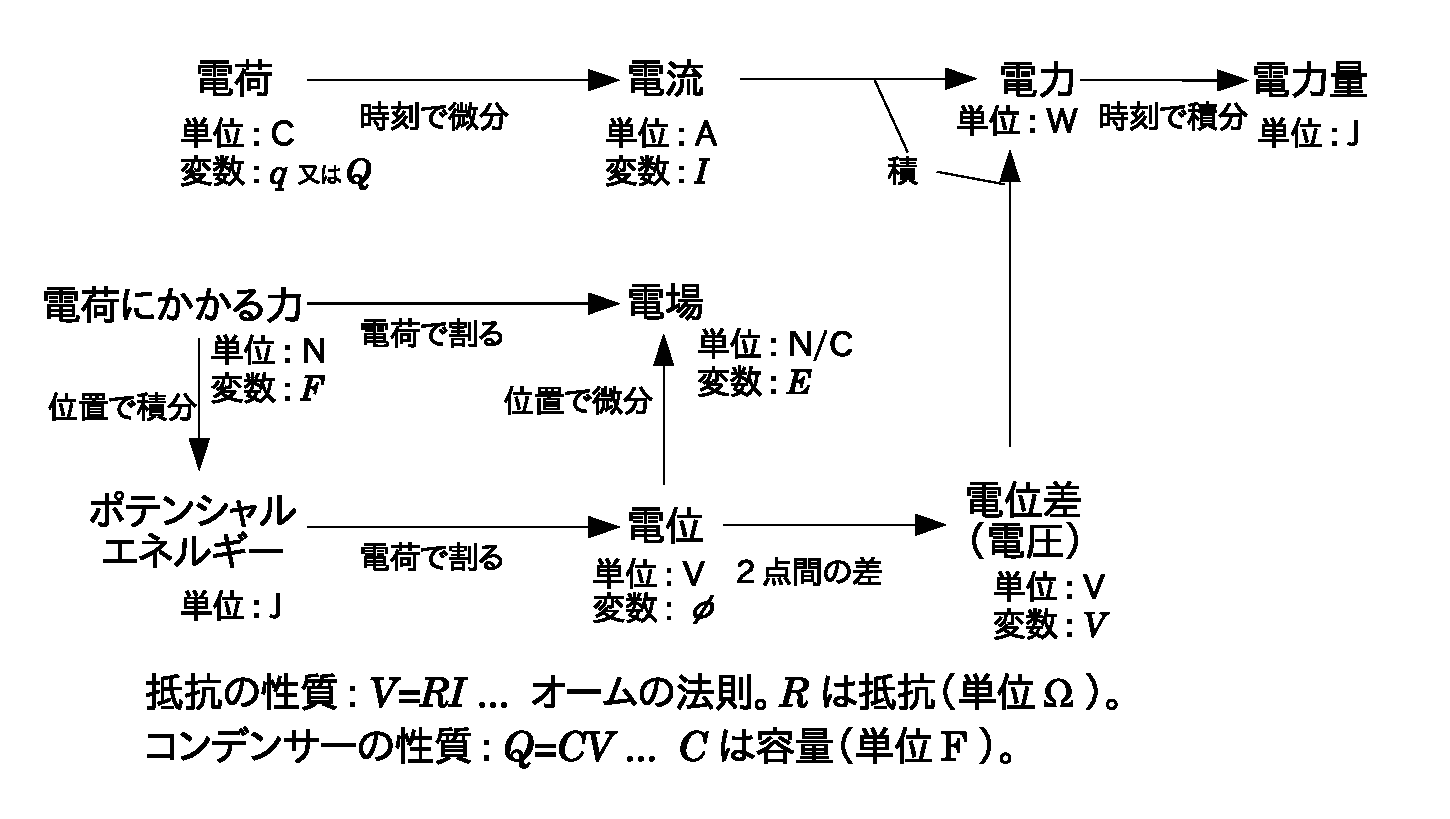
\includegraphics[width=8.5cm]{electronics.eps}
    \caption{電気に関する概念の関係図。斜字体と立体の区別に
注意せよ。斜字体は変数を, 立体は単位を表す。変数には, よく使われる
記号を示すが, 人によって例外もあることに注意せよ。単位の読み方
は, A: アンペア, C: クーロン, F: ファラド, J: ジュール, 
N: ニュートン, V: ボルト, W: ワット, $\Omega$: オーム}\label{fig:electronics}
\end{figure}

\begin{q}\label{eq:def_electricity} 電流・電力・電力量を, 
それぞれ簡潔に説明せよ。また, それぞれのSI単位を述べよ。
\end{q}\mv


\begin{q}\label{eq:battery_Ah} 電池の容量(電荷)を表すのに, A~h
という単位がよく使われる。ある自動車のバッテリー(8000円くらい)は, 
36A~hの容量だった。
\begin{enumerate}
\item このバッテリーが流すことのできる電荷の総量を求めよ。
\item このバッテリーができる仕事の総量を求めよ。ただし, この
バッテリーも含めて, 自動車のバッテリーはほとんどが電圧12~Vである。
\item ある車はこのバッテリーを積んでいる。この車のヘッドランプは
LEDであり, 片方が23~Wの消費電力である。左右両方のヘッドランプをつけっぱなし
にしたら, どのくらいの時間でバッテリーは空っぽになるか?
\end{enumerate}
\end{q}
\hv

\begin{exq} 昔は水田に水を入れるのに, 足踏み水車というものを使った。足踏み水車を使って, 
灌漑水路から水田(面積1~a)に水を入れようと思う。灌漑水路の水面と水田の
間には畦があり, 畦は水路水面よりも50~cm高い。この水田に, 水深5~cmになるまで水を
5時間で汲み上げる場合の仕事率を求めよ。\end{exq}
%1.4W

\begin{exq} 頂角60度の円錐があり、そこに質量100~gの円形の鎖がかぶさっている。
この鎖にかかる張力の大きさを求めよ。ただし円錐表面と鎖の間には摩擦は無い(つるつるしている)
とする。重力加速度は$g$=9.8~m~s$^{-2}$とする。\end{exq}


\section{解答}
% 
\noindent{\textbf{答}}\ref{q:def_work}
\begin{enumerate}
\item 力と, その力が働く点が力と同じ向きに動いた距離との, 積。
\item J = N~m=kg~m$^2$~s$^{-2}$。
\item 力がつりあっている系では, 仮想的な微小変位に伴って外力のなす仕事の総和は0である。
\end{enumerate}
\vspace{0.2cm}

% 
\noindent{\textbf{答}}\ref{q:teko}
\begin{enumerate}
\item 略(ヒント: 直角三角形の高さを三角関数で表す)。
\item 物体1について, 重力は鉛直下向きで$m_1g$である。その重力が働く
点である物体1の, 重力方向(鉛直下向き)への変位\footnote{位置の変化量
のことを変位(displacement)という。}は$h_1$であり, それは前問より$l_1\sin\theta$
である。従って, 重力が物体1にした仕事は
\begin{eqnarray}m_1gh_1=m_1gl_1\sin\theta\end{eqnarray}

物体2については, 重力は鉛直下向きで$m_2g$である。物体2の重力の方向
(鉛直下向き)への変位は$-h_2$である(マイナスがつくのは, 重力とは逆向きだから)。
それは前問より$-l_2\sin\theta$
である。従って, 重力が物体2にした仕事は
\begin{eqnarray}-m_2gh_2=-m_2gl_2\sin\theta\end{eqnarray}
\item 仮想仕事の原理より, 前問の2つの仕事の和は0だから, 
\begin{eqnarray}m_1gl_1\sin\theta-m_2gl_2\sin\theta=0\end{eqnarray}
従って, 
\begin{eqnarray}m_1l_1=m_2l_2\end{eqnarray}
\end{enumerate}
\vspace{0.2cm}

%
\noindent{\textbf{答}}\ref{q:jack}
\begin{enumerate}
\item ハンドルをまわす距離は$2\pi r$。ハンドルを回す力は, ハンドルの移動(回転)の
方向と常に一致しており, その大きさは$F$。したがって, ハンドルを1回転させるときに回す手がなす仕事は, 
$2\pi r F$。
\item ハンドルが1回転するときに, 上載物は$\Delta y$だけ持ち上がる。このとき, 上載物にかかる
重力は, 下向き(上載物の移動とは逆方向)に$mg$の大きさでかかるから, 重力のなす仕事は, 
$-mg\Delta y$となる。
\item ハンドルが1回転することを微小な変位であるとみなせば, 仮想仕事の原理より, 
ハンドルを回す手がなす仕事と重力がなす仕事の和は0である。従って与式が成り立つ。
\item 前小問の式を$F=$のように変形すればよい。
\item 前小問の式に各数値を代入して, 23 N。これは約2~kgの物体にかかる重力, つまり, 
2リットル入りのペットボトルを直接持ち上げる程度の力である。ジャッキを使えば, 
それで1000~kgの上載物を持ち上げることができるのだ。
\end{enumerate}

% 
\noindent{\textbf{答}}\ref{q:energy}
仕事が形を変えた量, もしくは仕事に形を変えることができる量。
\vspace{0.2cm}

% 
\noindent{\textbf{答}}\ref{q:spring_work}
仕事の定義\eref{eq:work2}で$F(x)=-kx$とすれば, 
\begin{eqnarray}W=\int_{x_0}^{x_1}(-kx)\,dx=-\frac{1}{2}k(x_1^2-x_0^2)\end{eqnarray}
\vspace{0.2cm}

% 
\noindent{\textbf{答}}\ref{q:gas_work} 
\begin{enumerate}
\item シリンダーの内部は, 底面積$A$, 高さ$h$の筒形の空間である。従ってその体積は$V=Ah$。
\item 気体は圧力$P$でピストンを押し上げようとする。一般に, 一定の圧力がかかる面には, 
圧力かける面積という大きさの力がかかる。従って, この場合は気体はピストンを$PA$という力で
押し上げようとする。いま, 座標軸を鉛直上向きにとっているので, 上向きが正。従って, $F_1=PA$。
\item ピストンは静止しているので, ピストンにかかる力はつりあっていなければならない。
従って$F_1$を打ち消す力が外から働いているはずである。従って外力は$F_2=-F_1=-PA$。
\item ピストンの移動がゆっくり(つまりほとんど静止しているということ)なので, 
力のつりあいは維持されると考えてよい。外力がなす仕事$dW$は, 力$F_2$と変位$dh$の積である。
従って, 
\begin{eqnarray}dW=F_2\,dh=-PA\,dh\end{eqnarray}
\item 変化前の気体の体積は$V=Ah$, 変化後の気体の体積は$V+dV=A(h+dh)$である。これらの式
より, $dV=A\,dh$を得る。
\item 略。
\item 略。(\eref{eq:gas_work5}を積分すればよい。)
\item 状態方程式より, $P=nRT/V$。これを前小問の結果に代入すれば与式を得る。
\item 温度一定なので, 前小問の式より, 
\begin{eqnarray}
W&=&-nRT\int_{V_1}^{V_2}\frac{dV}{V}=-nRT\Bigl[\ln|V|\Bigr]_{V_1}^{V_2}\nonumber\\
&=&-nRT\ln \frac{V_2}{V_1}=nRT\ln \frac{V_1}{V_2}
\end{eqnarray}
注: 体積$V_1, V_2$はいずれも正なので, 対数の中の絶対値記号は結局は不要になる。
\item $n=1\,$mol, $R=8.31$ J~mol$^{-1}$ K$^{-1}$, $T=273$ K, $V_1/V_2=2$, $\ln 2=\log_e 2\fallingdotseq0.693$
を前小問に代入し, $W=1570$ J。(有効数字3桁)
\end{enumerate}
\vspace{0.2cm}

% 
\noindent{\textbf{答}}\ref{q:def_potential}
ある基準点から任意の位置$x$まで物体を運ぶときの仕事
を$W(x)$とするとき, $U(x)=-W(x)$で定義される関数$U(x)$を
ポテンシャルエネルギーという。
\vspace{0.2cm}

% 
\noindent{\textbf{答}}\ref{q:potential_spring}
\eref{eq:spring_work}で, $x_0=0$, $x_1=x$とおきなおせば, 
\begin{eqnarray}
U(x)=-W(x)=\frac{1}{2}kx^2
\end{eqnarray}
\begin{figure}[h]
    \centering
    \includegraphics[width=6cm]{stringPE.eps}
    \caption{バネのポテンシャルエネルギー}\label{fig:stringPE}
\end{figure}
グラフは図\ref{fig:stringPE}のようになる。

% 
\noindent{\textbf{答}}\ref{q:potential_gravity}
\eref{eq:work_gravity}で, $R_0=\infty$, $R_1=R$とおきなおせば, 
\begin{eqnarray}
U(R)=-W(R)=-\frac{GMm}{R}
\end{eqnarray}
\begin{figure}[h]
    \centering
    \includegraphics[width=6cm]{gravityPE.eps}
    \caption{万有引力のポテンシャルエネルギー}\label{fig:gravityPE}
\end{figure}
グラフは図\ref{fig:gravityPE}のようになる。

\noindent{\textbf{答}}\ref{q:potential_etc}
\begin{enumerate}
\item \eref{eq:potential_g}において, $m=2$~kg, $g=9.8$~m~s$^{-2}$, $h=10$~mとすれば, 
$U=196\,\,\text{J}\fallingdotseq 200$ J
\item 問\ref{q:YoungModulus}(3)より, バネ定数$k$は, $k=6.2\times10^4$~kg s$^{-2}$。
また, $x=0.001$~mとして, これらを\eref{eq:potential_spring}に代入すれば, $U=0.031$ J。
\item 地球の質量を$M$, 月の質量を$m$, 地球と月の距離を$x$とすれば, 
\begin{eqnarray*}
G&=&6.7\times10^{-11}\,\text{ m}^3\,\,\text{kg}^{-1}\,\,\text{s}^{-2}\\
M&=&6.0\times10^{24}\,\text{ kg}\\
m&=&7.3\times10^{22}\,\text{ kg}\\
x&=&4.0\times10^{8}\,\text{ m}
\end{eqnarray*}
これらを\eref{eq:potential_gravity}に代入して, $U=-7.3\times10^{28}$ J。
(ただし無限遠を基準点とする。)
\end{enumerate}
\mv

% 傾斜角$\theta$の滑らかな斜面に沿って, 質量$m$の物体を, 斜距離$L$だけ運びあげた。
\noindent{\textbf{答}}\ref{q:slope_lift_energy1}
物体にかかる重力を, 斜面に垂直な方向と, 斜面に平行な方向に分解して考える。
前者は斜面から受ける垂直抗力と釣り合って打ち消しあう。後者は
\begin{eqnarray}mg\sin\theta\end{eqnarray}
となる($\theta$は傾斜角)。誰かがこれと等しい大きさの力を斜面に平行で上向きに
かけることで物体が斜距離$L$だけ移動する。そのとき「誰か」が行った仕事は, 
\begin{eqnarray}mgL\sin\theta\end{eqnarray}
となる。これはポテンシャルエネルギーの変化にも等しい。\mv


% 保存力とは何か? 
\noindent{\textbf{答}}\ref{q:conservative_force}
保存力とは, 物体をある位置から別の位置に運ぶときに
その力がなす仕事が, 移動の経路によらずに一定である, というような力である。\mv


% 摩擦力が保存力でないことを証明しよう。
\noindent{\textbf{答}}\ref{q:friction_non_conservative}
\begin{enumerate}
\item 物体を位置$x_0$から位置$x_1$に運んで位置$x_0$に戻す, という
移動も, 物体を位置$x_0$に置いたまま動かさない, というのも, ともに, 
「物体を位置$x_0$から位置$x_0$に移動する」経路である。前者の
仕事は$W_{01}+W_{10}$であり, 後者の仕事は0である(移動距離が無いから)。
従って, もし力が保存力なら, $W_{01}+W_{10}=0$である。
\item 動摩擦力の大きさを$F_{\text m}$とし, $x_0$と$x_1$の間の距離を$X$とすると, 
$W_{01}=-F_{\text m}X$である。ここでマイナスがつくのは, 力の向きが移動方向と
逆だからである。同様に, $W_{10}=-F_{\text m}X$である。従って, 
$W_{01}+W_{10}=-2F_{\text m}X$
となり, 前小問の式は成り立たない。従って摩擦力は保存力でない(背理法)。
\end{enumerate}
\mv

% 
\noindent{\textbf{答}}\ref{q:slope_lift_energy2}
問\ref{q:slope_lift_energy1}とほぼ同様だが, この場合, 物体には, 
斜面平行・下向きに, $\mu'mg\cos\theta$という摩擦力もかかる。そのぶん
「誰か」はがんばらねばならない。結果的に, 「誰か」が斜面に平行で上向きに
かける力は, 
\begin{eqnarray}mg\sin\theta+\mu'mg\cos\theta\end{eqnarray}
となる。
物体は斜距離$L$だけ移動するので, 「誰か」が行った仕事は, 
\begin{eqnarray}mgL\sin\theta+\mu'mgL\cos\theta\end{eqnarray}
となる。ところが, 摩擦力は保存力ではないので, ポテンシャルエネルギーの増減には
関与しない。従って, ポテンシャルエネルギーの増加は, $mgL\sin\theta$。\mv

\noindent{\textbf{答}}\ref{q:work_rate}
\eref{eq:work_rate_lift}に, $m=2.0$~kg, $g=9.8$~m~s$^{-2}$, $v=3.0$~m~s$^{-1}$を代入すると, 
有効数字2桁で$P= 59$ W。
\mv

%
\noindent{\textbf{答}}\ref{q:watt_hour}
1 W h = 1 J s$^{-1} \times 3600$ s=3600 J
\mv


\noindent{\textbf{答}}\ref{q:potential_Coulomb}
原点に電荷$Q$を固定し, $x$軸上に電荷$q$を動かす。位置$x$に電荷$q$があるとき($0<x$とする), 
それに働く力$F$は, \eref{eq:coulomb}より, 
\begin{eqnarray}
F=\frac{k\,Q\,q}{x^2}
\end{eqnarray}
である。無限遠から位置$x$まで電荷$q$を動かすときに, この力がなす仕事は, 
\begin{eqnarray}
W=\int_{\infty}^{x}F\,dx=\int_{\infty}^{x}\frac{k\,Q\,q}{x^2}\,dx
=\Bigl[-\frac{k\,Q\,q}{x}\Bigr]_{\infty}^{x}=-\frac{k\,Q\,q}{x}\nonumber\\\label{eq:potential_Coulomb00}
\end{eqnarray}
となる。\eref{eq:potential}より, 
\begin{eqnarray}
U(x)=-W=\frac{k\,Q\,q}{x}
\end{eqnarray}
となる(証明終わり)。\mv

{\small 注: \eref{eq:potential_Coulomb00}で, 積分変数$x$(つまり$dx$の$x$)と, 
積分区間の上端の$x$(つまり$\int_{\infty}^x$の$x$)が「かぶっている」が, 
これは別物と解釈する。すなわち積分変数$x$は, ほんとうは$X$とか$s$とか, 
何か適当に$x$以外の記号で置くのが数学的には正しいところだが, それは
めんどくさいしわかりにくくなるので, 横着して$x$のままにしておくのだ。このような
書き方は物理学でよく出てくる。\mv}

\noindent{\textbf{答}}\ref{q:potential_Coulomb2} 
\begin{enumerate}
\item \eref{eq:potential_Coulomb}を位置$x$における電荷$q$で割ればよい。
\begin{eqnarray}
\frac{U(x)}{q}=\frac{k\,Q}{x}\label{eq:voltage_Coulomb}
\end{eqnarray}
\item $x=0.529\times10^{-10}$~mとする。陽子の電荷は電荷素量なので
$Q=1.602\times10^{-19}$~C。また, \eref{eq:coulomb}より, 
$k=8.987\times 10^{9}$ N~m$^2$ C$^{-2}$。
これらを\eref{eq:voltage_Coulomb}に
代入すると, 27.2~V。
\end{enumerate}

\noindent{\textbf{答}}\ref{q:potential_Volt} 
\begin{enumerate}
\item 単位電荷あたりのポテンシャルエネルギー
\item 空間の2つの点の間を仮想的に荷電粒子を移動させるとき, 
かかる仕事を電荷で割ったもの。多くの場合, 2点間の電位の差(電位差)。
\item J~C$^{-1}$, 言い換えると, V。
\item 0.6~J
\item 電子の電荷は$-1.602\times10^{-19}$ Cなので, それが1~Vの電位にあると, 
$-1.602\times10^{-19}$ J。
\end{enumerate}
\mv


\noindent{\textbf{答}}\ref{q:radiation_eV}
\begin{enumerate}
\item $m_{\text{He}}=4$~g$/(6.0\times10^{23})$=...=6.7$\times10^{-27}$~kg。
\item $\alpha$線のエネルギーを$E$, 速さを$v$とすると, $\frac{1}{2}m_{\text{He}}v^2=E$。
従って, $v=\sqrt{2E/m_{\text{He}}}=...=1.6\times10^7$~m~s$^{-1}$。
\item $\beta$線のエネルギーを$E$, 速さを$v$とすると, 上と同様に, 
従って, $v=\sqrt{2E/m_{\text{e}}}=...=4.2\times10^8$~m~s$^{-1}$。
\end{enumerate}
注: eVをJに直して計算しないと, 正しい答にはならない。単位を埋め込んで計算すれば, 
それに気がつくはず!
\mv

%\noindent{\textbf{答}}\ref{eq:def_electricity} 略。
%\mv

\noindent{\textbf{答}}\ref{eq:battery_Ah} 
\begin{enumerate}
\item 36~A~h=36~(C/s)$\times$3600~s=130000~C。
\item 12~V$\times$36~A~h=$12\times36\times3600$~V~A~s=$1.6\times10^6$~J。
\item 左右両方で46~W。12~Vの電圧では, 46~W/(12~V) =3.8~Aの電流が
流れる。36~A~h/(3.8~A) =9.4~h。およそ9時間で空になる。これがLEDでなく, 
普通のハロゲンランプなら, もっと短い時間(数時間)で空になってしまう。
\end{enumerate}


\begin{faq}{\small\textgt{本当なのかなーって疑いたくなる値が答えだったり, 物理ってなんなんだー}
... 皆さんの既成概念を壊すために, そういうのを狙って問題を作ってます。}\end{faq}\mv

\begin{faq}{\small\textgt{代入する値がほしいです。}
 ... そのうち, 文字(変数)だけの答えにも慣れますよ。そっちのほうが, 
いろんな量どうしの関係がわかりやすい。}\end{faq}\mv

\begin{faq}{\small\textgt{「示せ」という問題は文も必要ですか? 言葉での説明が苦手です。}
 ... 言葉の定義をしっかり把握してください。その上で, まずは自分自身で納得できる説明を探すことが重要。}\end{faq}\mv

\begin{faq}{\small\textgt{なんとなくわかるけど, 問題解くときにわけわからなくなります。}
... だから問題演習は大事。しっかり考えて, わからなければ解答を読んで, また考えて下さい。}\end{faq}\mv


\chapter{運動の三法則}\label{chapt:motionlaw}

{\small 注: この章を学ぶには「微分」「ベクトル」「微分方程式」を理解していることが必要である。}\\

これから我々は物体の運動に関する物理学を学ぶ。「物体の運動」とは, 
物体の位置や向きや形状が時刻とともに変化する様子である。
とはいうものの, 当面は「位置」だけに着目し, 「向き」や「形状」
については難しすぎるので後回しにする。そのために我々は
まず物体を質点としてモデル化し, 質点の運動を考える。

\begin{faq}{\small\textgt{てことは, 物体が変形したり回転したり
する様子はわからない, ってことですか? そんなのしょぼ過ぎません?}
... 大丈夫。質点の運動をきっちり理論化できたら, それを使って
変形や回転なども理論化できます(そのうち学びます)。物事には順序
というものがあるのです。}\end{faq}

というわけで, 我々の当面の目標は, 質点の位置を時刻の関数として
表すことだ。それには, ベクトル, 微分, 積分という3つの数学を駆使する。
まずその準備をしよう。\\


\section{ベクトルとスカラー}

中学校理科で学んだように, 速度や力は, 「向き」と「大きさ」を持つ。
このように, 向きと大きさを持つ量のことを「ベクトル」と呼ぶ(定義)。
それに対して, 大きさだけを持ち向きを持たない(ただしプラスとマイナスは
あってもよい)ような量を「スカラー」と呼ぶ(定義)。例えば力はベクトルだが, 
「力の大きさ」はスカラーである。

ベクトルを記号で表すときは, 高校では$\vec{F}$とか$\vec{v}$の
ように, 「アルファベットに上付き矢印」を使っていたが, 大学では, 
${\bf F}$とか${\bf v}$のように, 「アルファベットの太字」
を使う(慣習)。それに対して, スカラーは, 上矢印もつけず, 太字でもない, 
普通の細字のアルファベットで表す(慣習)。

ベクトルとスカラーをきっちり区別しないと, 数学的な取り扱い
で大きなミスをする可能性がある。そこでこのように, 
\begin{itembox}{慣習}
ベクトルの記号は太字\\
スカラーの記号は細字
\end{itembox}
で書き分けるのである。

物理学では, 質点の位置もベクトルとして表す。すなわち, まず空間の
どこかに「原点」を設定し, この原点から見た「向き」と「距離」で, 位置を
表す。そう考えるといろいろ便利だからである。

そのようなベクトルを「位置ベクトル」という。位置ベクトルは, 慣習的
に${\bf r}$で表すことが多い。

ベクトルは, 3次元空間の中の座標軸の方向, 
すなわち$x$方向, $y$方向, $z$方向のそれぞれの大きさ
(の組み合わせ)として表すこともできる。そういうのを「成分」
という。例えば, ${\bf F}$を力のベクトルとすると, これは
\begin{eqnarray}
{\bf F}=(F_x, F_y, F_z)\label{eq:FFxFyFz}
\end{eqnarray}
のように, 3つの成分$F_x$, $F_y$, $F_z$の組み合わせ
で表すことができる。

ベクトルの成分はスカラーである(向きがあらかじめ決められているので, 
大きさしか意味を持たない)。従って成分は細字で書かねば
ならない。つまり, \eref{eq:FFxFyFz}の左辺の${\bf F}$は太字であり, 
右辺の$F_x$, $F_y$, $F_z$は細字である。\eref{eq:FFxFyFz}を, 
\begin{eqnarray*}
&&F=(F_x, F_y, F_z)\quad\quad\text{と書いてはダメだし, }\\
&&{\bf F}=({\bf F}_x, {\bf F}_y, {\bf F}_z)\quad\quad\text{と書いてもダメ}
\end{eqnarray*}
である。\mv

\begin{faq}{\small\textgt{力はベクトルなので, 太字で書かなきゃ
ダメなんですよね。でも, 前の章では, $F=-kx$みたいに, 細字で
書いてましたが...?} ... それはバネに関するフックの法則ですね。
バネは普通, 1方向にしか伸び縮みしません。その方向に$x$軸をとり, 
それに垂直な方向に$y$軸, $z$軸をとれば, 力${\bf F}$は
\begin{eqnarray}
{\bf F}=(F_x, 0, 0)
\end{eqnarray}
と書けますね($x$軸方向以外の成分はいつもゼロ)。てことは, $y$方向
や$z$方向のことを気にする必要が無いから, 改めて$F_x$を$F$と書いて, 
\begin{eqnarray}
{\bf F}=(F, 0, 0)
\end{eqnarray}
と書いても差し支えありません。で, この$x$成分を取り出したのが, 
$F=-kx$の左辺の$F$なのです。すなわち, 常にひとつの方向(ひとつの直線の上)
に限定された現象を考える場合は, その方向での成分だけをいきなり
取り出して, 細字で書くのが普通です。これは慣習的なことですが, 
学生がよく混乱するので, 大きく書いておきましょう:
\begin{itembox}{慣習}
直線上に限定した議論や問題では, ベクトルであっても細字記号を使う。
\end{itembox}
}\end{faq}


\section{位置・速度・加速度}

\underline{位置を時刻で微分したものを速度という(定義)}。また, 
\underline{速度を時刻で微分したものを加速度という(定義)}。これらを数式で表現してみよう:

まず, 時刻を$t$とし, 質点の位置を
\begin{eqnarray}
{\bf r}(t)=(x(t), y(t), z(t))
\end{eqnarray}
とする。以後, $(t)$は, 「これは$t$の関数だ」というしるしであり, \textgt{時には省略されることもある}。

また, 質点の速度を
\begin{eqnarray}
{\bf v}(t)=(v_x(t), v_y(t), v_z(t))
\end{eqnarray}
とし, 質点の加速度を
\begin{eqnarray}
{\bf a}(t)=(a_x(t), a_y(t), a_z(t))
\end{eqnarray}
とする。そして速度と加速度を, それぞれ
\begin{eqnarray}
&&{\bf v}(t)=\frac{d}{dt}{\bf r}(t)\label{eq:v_drdt}\\
&&{\bf a}(t)=\frac{d}{dt}{\bf v}(t)=\frac{d^2}{dt^2}{\bf r}(t)\label{eq:a_dvdt}
\end{eqnarray}
と定義する。

\begin{faq}{\small\textgt{この$\frac{d}{dt}$って何ですか?}
 ... 変数$t$で微分する, という意味の記号です。}\end{faq}

\eref{eq:v_drdt}を各成分にわけて書き改めると, 以下のようになる:
\begin{eqnarray}
&&v_x(t)=\frac{d}{dt}x(t)\label{eq:def_vx_dxdt}\\
&&v_y(t)=\frac{d}{dt}y(t)\label{eq:def_vy_dydt}\\
&&v_z(t)=\frac{d}{dt}z(t)\label{eq:def_vz_dzdt}
\end{eqnarray}
また, \eref{eq:a_dvdt}を各成分にわけて書き改めると, 以下のようになる:
\begin{eqnarray}
&&a_x(t)=\frac{d}{dt}v_x(t)=\frac{d^2}{dt^2}x(t)\label{eq:def_ax_dvdt}\\
&&a_y(t)=\frac{d}{dt}v_y(t)=\frac{d^2}{dt^2}y(t)\\
&&a_z(t)=\frac{d}{dt}v_z(t)=\frac{d^2}{dt^2}z(t)
\end{eqnarray}

さて, ここで, これからよく使う公式を導出しておこう。
「解析学の基本定理」(数学の教科書参照)によれば, 
微分可能な関数$f(t)$について, 
\begin{eqnarray}
\int_a^x\frac{d}{dt}f(t)\,dt=f(x)-f(a)\label{eq:ftsekibun00}
\end{eqnarray}
が成り立つ。ここで, $a=0$とおいて変形すると, 
\begin{eqnarray}
f(x)=f(0)+\int_0^x\frac{d}{dt}f(t)\,dt
\end{eqnarray}
となる。ここで, $x$を形式的に$t$と置き直す。つまり, 積分区間の
上端の$t$と積分変数の$t$が「かぶる」ことになる(これが気持ち悪いという
人は, 答\ref{q:potential_Coulomb}の解説を参照しよう)。すると, 
\begin{eqnarray}
f(t)=f(0)+\int_{0}^{t}\frac{d}{dt}f(t)\,dt\label{eq:ftsekibun}
\end{eqnarray}
となる。

さて, \eref{eq:ftsekibun}で$f$を$x$で置き換えれば(これは
\eref{eq:ftsekibun00}で出てきた$x$とは無関係), 
\begin{eqnarray}
x(t)&=&x(0)+\int_{0}^{t}v_x(t)\, dt\label{eq:xfromvx}
\end{eqnarray}
となる。ここで\eref{eq:def_vx_dxdt}を使ったことに注意。

同様に, \eref{eq:ftsekibun}で$f$を$v_x$で置き換えて考えれば, 
\begin{eqnarray}
v_x(t)&=&v_x(0)+\int_{0}^{t}a_x(t)\, dt\label{eq:vxfromax}
\end{eqnarray}
となる。ここで\eref{eq:def_ax_dvdt}を使ったことに注意。

\eref{eq:xfromvx}, \eref{eq:vxfromax}のような式は, 
${\bf r}$や${\bf v}$の$y$成分と$z$成分についても成り立つので, まとめて
以下の式が成り立つ:
\begin{eqnarray}
{\bf r}(t)&=&{\bf r}(0)+\int_{0}^{t}{\bf v}(t)\, dt\label{eq:rfromv_vec}\\
{\bf v}(t)&=&{\bf v}(0)+\int_{0}^{t}{\bf a}(t)\, dt\label{eq:vfroma_vec}
\end{eqnarray}
これらの式を駆使して, いくつかの典型的な運動を表してみよう。
\hv

\begin{faq}{\small\textgt{$x$を$t$で置き換えて, また$f$を$x$で置き換えて, 
って, そんな勝手なことしていいのですか?} ... いいのです。これらは
形式的な置き換えに過ぎません。}\end{faq}
\begin{comment}
\begin{faq}{\small\textgt{いきなり微分と積分がガンガン出てきてびっくりです。
これが物理なのですか? 数学じゃないですか!} ... だから言ったでしょ, 
物理は数学をガンガン使うって。}\end{faq}

\begin{faq}{\small\textgt{勘弁して欲しいです。数学ナシでやってもらえませんか?}
... 「数学ナシの物理」の方が苦行です。数学を使うほうが, 本質的に, 正確に, 楽に
物理を表現できるのです。}\end{faq}

\begin{faq}{\small\textgt{私は高校生物学の教員免許が欲しいだけです。数学は
ガチで勘弁して欲しいのです。}
... 「高校生物学の教員免許」なんてものはありません。あるのは「高校理科の教員免許」
です。それには漏れなく物理が付いてくるのです。そして物理には数学が漏れなくついて
くるのです(笑)。それが嫌なら, 予備校の生物学の先生になればいいのでは?}\end{faq}

\begin{faq}{\small\textgt{高校物理では微積分は使わないのだから, 高校理科の
教員免許のためならば, 物理で微積分を使う必要は無いのでは?}
... 微積分を理解しない人は, 物理は公式の羅列と当てはめにすぎない, 
と考える傾向があります。そういう浅はかな考えの人に習う生徒が迷惑です。
}\end{faq}
\end{comment}


\section{等速直線運動}\index{とうそくちょくせんうんどう@等速直線運動}

まず最もシンプルな運動を考えよう。

速度${\bf v}=(v_x, v_y, v_z)$が(向きも含めて)一定であるような運動\footnote{ここではあえて
教育的に「向きも含めて」と書いたが, そもそも速度は, 大きさと向きを持つ
ベクトルなので, 「速度が一定である」と言えば, 向きも含めて一定
であることを自動的に意味する。}を「等速直線運動」という(定義)。
この場合, $v_x$は$t$によらない定数である。この場合は\eref{eq:xfromvx}の積分は簡単にできて, 
\begin{eqnarray}
x(t)&=&x(0)+\int_{0}^{t}v_x\, dt\nonumber\\
&=&x(0)+[v_x\,t]_{0}^{t}\nonumber\\
&=&x(0)+v_x\,t
\end{eqnarray}
となる。同様のことが$y$成分, $z$成分でも言えるので, 
\begin{eqnarray}
&&x(t)=x(0)+v_xt\label{eq:constantvelocity_x}\\
&&y(t)=y(0)+v_yt\label{eq:constantvelocity_y}\\
&&z(t)=z(0)+v_zt\label{eq:constantvelocity_z}
\end{eqnarray}
となる。これらをまとめて, 
\begin{eqnarray}
{\bf r}(t)={\bf r}(0)+{\bf v}\,t
\end{eqnarray}
と書くこともできる。この式から, 
${\bf r}$が, 点${\bf r}(0)$を通り, 方向ベクトルが${\bf v}$であるような直線を描くことが
わかる。すなわち, 等速直線運動は, 確かに「直線」の上を運動する。\mv

ここで, 速度が${\bf 0}=(0, 0, 0)$で一定の状況を考えよう。
その場合も「速度一定」なのだから等速直線運動なのだが, 実際は
質点は静止している。つまり, 「静止状態」は「等速直線運動」の
一例なのだ。\mv

\begin{faq}{\small\textgt{${\bf 0}=(0, 0, 0)$は, 単位をつけなくて
よいのですか? 「速度0」は正しくは「速度0~m/s」じゃないですか?}
... 単位をつけたければつけてもよいですが, 0には単位は不要です。
物理量は数値$\times$単位です。単位に0がかかるのだから単位も消えて0です。
それに, 0~m/sも0~cm/sも0~km/hも同じでしょ? なら, 単位をつける意味, ないですよね?
}\end{faq}
\hv


\section{等加速度直線運動}\label{sect:const_accel}
\index{とうかそくどちょくせんうんどう@等加速度直線運動}

次にシンプルなのは, 速度は変わるが加速度は一定, という運動である。
そのような運動を「等加速度直線運動」という(定義)。

この場合, $a_x$は$t$によらない定数であり, \eref{eq:vxfromax}の積分は
「定数の積分」だから簡単にできる。その結果は, 
\begin{eqnarray}
v_x(t)&=&v_x(0)+\int_{0}^{t}a_x\, dt=v_x(0)+[a_x\,t]_{0}^{t}\nonumber\\
&=&v_x(0)+a_x\,t\label{eq:constacc_vx}
\end{eqnarray}
となる。これを\eref{eq:xfromvx}に代入すると, 
\begin{eqnarray}
x(t)&=&x(0)+\int_{0}^{t}v_x(t)\, dt\nonumber\\
&=&x(0)+\int_{0}^{t}(v_x(0)+a_x\,t)\, dt\nonumber\\
&=&x(0)+\Bigl[v_x(0)\,t+\frac{1}{2}a_x\,t^2\Bigr]_0^t\nonumber\\
&=&x(0)+v_x(0)\,t+\frac{1}{2}a_x\,t^2\label{eq:constacc_x}
\end{eqnarray}
となる。すなわち, 加速度一定の運動は, 時刻の2次関数で表されるのだ。
この具体例を, 後ほど学ぶ。さて上の式と同様のことが$y$成分, $z$成分
でも言えるので, まとめて, 
\begin{eqnarray}
{\bf v}(t)&=&{\bf v}(0)+{\bf a}\,t\label{eq:constacc_v5}\\
{\bf r}(t)&=&{\bf r}(0)+{\bf v}(0)\,t+\frac{1}{2}\,{\bf a}\,t^2\label{eq:constacc_r5}
\end{eqnarray}
と書くこともできる。これらの式は, 高校物理でも出てくるが, 実は
「しょぼい」式である。なぜならば, \textgt{これらは「加速度が一定」
という特殊な条件でしか使えない}のだ。普遍性・一般性に乏しいのだ。

ではもっと複雑な運動はどういう式になるだろう? それは加速度が時間
とともに変わるような運動である。それを理解するには, 次節の話が欠かせない。\mv

\begin{faq}{\small\textgt{高校物理では, \eref{eq:constacc_vx}と
\eref{eq:constacc_x}を公式として記憶させられました。やっぱ覚えるべき
でしょうか?} ... こんなしょぼい式を暗記しても仕方ないし, どうせ忘れます。
それよりも, 微積分の考え方を理解して, この式を自力で導けるようにする
方が重要です。}\end{faq}

\begin{q}\label{q:constaccel} 以上の解説を参考にして, 
\eref{eq:constacc_vx}, \eref{eq:constacc_x}の導出を再現せよ。\end{q}
\mv


\section{運動の三法則}

前々章で, 力に関する法則について述べた。ではそもそも力とは
何なのだろうか? 力は自然界に何をもたらすのだろうか? 
端的に言えば, 力は, 物体の運動に変化をもたらすものだ。それを支配する
のが以下の, ニュートンの「\underline{運動の三法則}」\index{うんどうのさんほうそく@運動の三法則}
だ。これらは必ず記憶しなければならない。
\begin{itembox}{運動の三法則}
\begin{itemize}
\item 第一法則:質点に働く合力が${\bf 0}$のとき, 質点は等速直線運動をする。
(慣性の法則)\index{かんせいのほうそく@慣性の法則}
\item 第二法則:質量$m$の質点に合力${\bf F}$がかかると, 質点は次式に従って運動する
(運動方程式)\index{うんどうほうていしき@運動方程式}:
\begin{eqnarray}
{\bf F}=m{\bf a}\label{eq:motion}
\end{eqnarray}
ここで, ${\bf a}$は質点の加速度である。
\item 第三法則:2つの質点A, Bにおいて, AがBに力を及ぼすとき, AはBから, 同じ大きさで
逆向きの力を及ぼされる。(作用・反作用の法則)\index{さようはんさようのほうそく@作用・反作用の法則}
\end{itemize}
\end{itembox}

%2011.4.2 ヤマサキ 2章で述べてある「力のつりあい」との関連がはっきりするように変更しました。
この「運動の三法則」も, 物理学における基本法則(根源的な原理)であり, 
なぜ成り立つのかは, 誰も知らない。しかし, 運動の三法則は, 歴史的にも理論体系
としても, 科学の根幹である。運動の三法則が発見されたとき, 人類は科学の扉を
大きく開いたのだ。これは知識人の教養である。\mv

第2章では, 「物体が静止している場合, その物体に働く力(合力)はゼロである」
と学んだ。注意して欲しいのは, その逆は必ずしも成り立たない, 
ということだ。すなわち, 「物体に働く力がゼロなら物体は静止する」
\underline{は成り立たないことがある}。例えば, 宇宙空間を飛んでいる
隕石は, 何かに引かれたり押されたりして飛んでいるわけではなく, 
それにかかる力が0でありながら, そのまま飛び続ける。そのように, 
「働く力がゼロ」でも物体が運動するケースがあるのだ。それを
包含するのが, この第一法則(慣性の法則)だ。第一法則によれば, 
「働く力がゼロ」のときに実現するのは「等速直線運動」だ。
前節で述べたように, 静止状態は等速直線運動の一例に過ぎない
(速度0での等速直線運動)。\mv

\begin{q}\label{q:motion1condition}「物体が静止している」を条件A, 
「物体が等速直線運動をしている」を条件B, 「その物体に働く力(合力)はゼロである」を条件Cとする。
\begin{enumerate}
\item AはCの必要条件? 十分条件? 必要十分条件? いずれでもない?
\item BはCの必要条件? 十分条件? 必要十分条件? いずれでもない?
\item BはAの必要条件? 十分条件? 必要十分条件? いずれでもない?
\end{enumerate}
{\small ヒント: 必要条件や十分条件がわからない人は, 数学の教科書を見よう!}
\end{q}
\mv

第一法則は中学校で習うが, これを正確に理解するのは簡単ではない。特に, \\
  \textgt{「力がかからなくても物体は動く」} ....... (*)\\
と言うと, 多くの人が驚いた顔をする。これは多分に言葉の解釈の
問題である。というのも, 「動く」には, 
\begin{itemize}
\item 「(止まっていたものが)動き始める」
\item 「動いている状態にいる」
\end{itemize}
という2つの解釈がある。前者の意味に解釈すると, 確かに(*)はおかしい, 
間違った命題だ。止まっている物体が動き始めるには, 力が必要だ。
第一法則が言っているのは, 後者の意味だ。既に運動状態にある物体は, 
さらに押したり引いたりしてあげなくても, 放っといてもその運動状態
(それは等速直線運動)を続けるのだ。\mv

第一法則は, その対偶をとって「質点が等速直線運動以外の運動をするとき, 
質点に働く合力は${\bf 0}$ではない」と言い換えることもできる(対偶とは
何かがわからない人は, 数学の教科書で調べよ)。

\begin{exmpl} 質点が, ある円の周上を, 一定の速さ(速度ではない!)で
まわるような運動を考える(それを「等速円運動」という)。そこでは, 速度の
大きさ(つまり速さ)は一定でも速度の方向が時々刻々と変化するので, 
「等速直線運動」ではない。従って, 等速円運動では, 必ず何らかの力
(${\bf 0}$でない合力)が質点にかかっている。後に学ぶが, それを
「向心力」という。(例おわり)\end{exmpl}

\begin{q}\label{q:escalator} エスカレーターで「手すりにおつかまり下さい」
と言われるのはなぜか? 慣性の法則の観点で説明せよ。ヒント: 手すりを持たないと, 
上りよりも下りの方が危ない。\end{q}\mv

さて, 等速直線運動以外の運動も扱うのが次の第二法則だ。
第二法則(運動方程式)は, 君が1学期の物理学で学ぶべき\underline{最も重要な法則}だ。
君はその威力を, これから少しずつ実感するだろう。

\eref{eq:motion}で${\bf F}$と${\bf a}$はベクトルである。つまり大きさと方向を持つ。成分で書いて, 
\begin{eqnarray}
{\bf F}&=&(F_x, F_y, F_z)\\
{\bf a}&=&(a_x, a_y, a_z)
\end{eqnarray}
とすれば, 方程式(\ref{eq:motion})は, 
\begin{eqnarray}
F_x=ma_x,\quad
F_y=ma_y, \quad
F_z=ma_z
\end{eqnarray}
という3つの方程式と同じことだ。

\eref{eq:motion}は, 左辺と右辺を入れ替えて次式のように表される
こともあるが, 正直, どちらでもよい:
\begin{eqnarray}
m{\bf a}={\bf F}\label{eq:motion_ma_F}
\end{eqnarray}

\begin{faq}{\small\textgt{高校の先生は, ${\bf F}=m{\bf a}$ではなく
$m{\bf a}={\bf F}$だ, と言っていましたが。。。} ...
そういう人はいます。曰く, 物理学では等号の左辺と右辺で意味は違うのだ, 
とのこと。でもそのような約束はその人が自分の世界観や物理観をもとに
勝手に作ったものに過ぎません。数学では等号は左右を入れ替えても成り立つ
と約束されているし(等号の公理), 物理学の法則は数学で記述される
のだから, ${\bf F}=m{\bf a}$と$m{\bf a}={\bf F}$は厳密に同じであり, 
どちらも正しいです。}\end{faq}

方程式(\ref{eq:motion})は, \eref{eq:a_dvdt}を使って, 以下のように
表されることも多い: 
\begin{eqnarray}
&&{\bf F}=m\frac{d{\bf v}}{dt}\label{eq:motion_df}\\
&&{\bf F}=m\frac{d^2{\bf r}}{dt^2}\label{eq:motion_df2}
\end{eqnarray}

式(\ref{eq:motion})から, 力は質量(SI単位はkg)と加速度(SI単位はm~s$^{-2}$)
の積と同じ単位を持たねばならぬ。だから, 力のSI単位がkg~m~s$^{-2}$になる
のであり, この単位をN (ニュートン)と呼ぶのだ。

さて, 式(\ref{eq:motion_df})(\ref{eq:motion_df2})を見ると, 運動方程式は, 位置や速度
に関する, \underline{微分方程式}\index{びぶんほうていしき@微分方程式}(関数の微分を含む方程式)
だとわかる。一般に, 微分方程式は, 未知の関数の方程式であり, 
それを「解く」ことによって未知だった関数が具体的に求まる。今の場合は, 
力${\bf F}$と, 初期値(ある時刻における位置と速さ)が具体的にわかれば, 
運動方程式が解ける。そしてその結果, 速度${\bf v}(t)$や位置${\bf r}(t)$という, 
時刻$t$に関する関数(ベクトル値関数)が, 全ての時刻$t$において
具体的に求まる。つまり, \underline{質点の運動の全てが数学的に決まってしまう}。
つまり, 運動方程式は, あらゆる質点の運動を予測する能力を秘めているのだ\footnote{その
ため, 運動方程式は人類に運命論的な世界観を突きつけることになった。}。

%2011.4.2 ヤマサキ 1章でやった「オッカムの剃刀」との関連がはっきりするように変更しました。
ところで, 式(\ref{eq:motion})で${\bf F}={\bf 0}$と置いてみよう。すると, ${\bf 0}=m{\bf a}$となる。
質量$m$が0でなければ, 結局, ${\bf a}={\bf 0}$だ。${\bf a}$は速度の微分なので, それが${\bf 0}$
ということは, 速度が(向きも含めて)時刻によらず一定, ということだ。つまり, 
働く力がゼロなら質点は等速直線運動をする, ということだ。これは第一法則(慣性の法則)と整合する。
つまり, 質点に力がかかる場合とかからない場合のどちらの場合も, 
第二法則で表現することができるわけだ。ということは, 第1章で学んだ「オッカムの剃刀」に従って, 
第一法則は削ってしまうべきではないだろうか?(運動の"二"法則の方が, 
"三"法則よりシンプルだ!) 
いや, それでもなお, 第一法則は削ってはならないのだ。このあたりは, いずれ
「慣性系」\index{かんせいけい@慣性系}という概念を学ぶときに詳述する\footnote{
藤原邦男「物理学序論としての力学」東大出版, p. 36-37参照。}。

また, 第三法則(作用・反作用の法則)は, 既に述べた。

運動の三法則や万有引力の法則は, ニュートンが発見した。これらの法則から導かれる物理学
(力学)を, ニュートン力学という。\mv

以上で, 力学の根源的な法則は終わりだ。あとは, これらの法則から導出される派生的な法則である。\mv

\begin{q}\label{q:Newton_3laws}
運動の三法則を3回書いて記憶せよ。(それぞれの名前だけでなく内容を! 
${\bf F}$と${\bf a}$は太字であることに注意!)
\end{q}

\begin{q}\label{q:NewtonLaw_mistake} 運動の三法則について, 
以下の記述それぞれについて, 正しいか, 正しくないか, 理由もつけて述べよ。
\begin{enumerate}
\item 質点Aが質点Bに力を及ぼすとき, AはBから, 同じ力を受ける。
\item 質点が等速直線運動をしているとき, 質点にかかる合力は${\bf 0}$である。
\item 質量$m$の質点に合力$F$がかかるとき, 質点の加速度を$a$とすると, $F=ma$が成り立つ。
\end{enumerate}
\end{q}
%答まだ。



ところで, 唐突だが, ここで\underline{運動量}\index{うんどうりょう@運動量}という
ものを以下のように定義する:
\begin{itembox}{運動量の定義}
$m$を質点の質量, ${\bf v}$を質点の速度とすると, 
\begin{eqnarray}{\bf p}=m{\bf v}\label{eq:def_momentum}\end{eqnarray}
を質点の運動量と呼ぶ。
\end{itembox}

すると, $m$を定数とみなせば, 運動方程式(\ref{eq:motion})は, 
\begin{eqnarray}
{\bf F}=\frac{d{\bf p}}{dt}\\
\frac{d{\bf p}}{dt}={\bf F}
\end{eqnarray}
などともあらわされる。これらはもちろん, 全て互いに同じ方程式である\footnote{ただし, 
$m$が一定でないような場合(光速に近い高速運動など)は, ${\bf F}=m{\bf a}$は成り立たなくても
${\bf F}=d{\bf p}/dt$は成り立つ。従って, ${\bf F}=m{\bf a}$より${\bf F}=d{\bf p}/dt$のほうが, 
より一般性の高い記述である。}。運動量という概念は, 後に大変重要な働きをする。\mv

\begin{q}\label{q:def_momentum}
運動量の定義を5回書いて記憶せよ。(${\bf p}$と${\bf v}$は太字であることに注意!)
\end{q}
\mv

\begin{faq}{\small\textgt{サッカーで, 「長友佑都の驚異の運動量」とかよく言いますが, 
あれのことですか?} ... わかります。長友選手は疲れ知らずでよく走り回る, という意味ですね。
でも, 違います。物理学用語の「運動量」は, それとは全く違うことを意味します。}\end{faq}

\begin{faq}{\small\textgt{運動量の定義について。「${\bf p}$を運動量, $m$を質量, 
${\bf v}$を速度とする。${\bf p}=m{\bf v}$が成り立つ」と書いたら, なんかダメっぽい
ことを言われました。なんで?」} ... これは, 「が成り立つ」がダメなのです。
そこを「とする」とか「と定義する」と書けばOKでした。

「成り立つ」は「そうなる」ということです。ところが, ここでは定義を述べています。
${\bf p}=m{\bf v}$は「そうなる」のではなく, 「そうする」「そう決める」
「そう約束する」「そう定義する」ものなのです。運動量${\bf p}$の意味や正体が, 
この式によって初めて定まるのです。

こういうところで「成り立つ」を使ってしまうと, あたかも運動量${\bf p}$が
別のところで別の意味として定義され, そしてそれが, 何かの理論や奇跡に
よって, $m{\bf v}$と等しいことが確かめられた! みたいに受け取られます。

言葉尻を捉えているように思うかもしれませんが, これは大事なことです。
科学を体系的に理解する時, 定義(約束), 基本法則(理由なく認めざるを
得ない自然現象のルール), 定理(定義や基本法則から理論的に導かれる
もの)を, はっきりと区別しなければなりません。その際, まず重要なのは, 
それが「成り立つ」ようなもの(だとしたら基本法則か定理)なのか, 
それとも「そう約束する」ようなものなのか(だとしたら定義), です。}\end{faq}
\mv

では, 以下, 具体的な運動について運動方程式を解いてみよう。なお, この章で出てくる問は
すべて一直線上の運動なので, 力や位置や速度や加速度はスカラーと考えてよい
(あえて3成分のベクトルとして考える必要はない)。次章以降ではベクトルとして考える必要が出てくる。
\hv


\section{力が一定の運動}

まず, 力が時間と共に変わったりせず, 常に一定であるような状況で起きる運動
を考えよう。その場合, 第二法則から, 加速度も
一定であるということがわかる。そのような運動は, \pref{sect:const_accel}で
学んだ「等加速度直線運動」になる。

その最も身近な例は, 重力に任せて落ちていく運動, すなわち「自由落下」
\index{じゆうらっか@自由落下}である。

\begin{q}\label{q:freefall0}
地表付近で重力だけを受けて上下運動をする, 質量$m$の質点の運動を考える。
重力加速度を$g$, 時刻を$t$とする。地表から鉛直上向きに$x$軸をとる。
時刻$t$における質点の位置, 速度, 加速度を, それぞれ$x(t), v(t), a(t)$とする。
初期条件は
\begin{eqnarray}x(0)=x_0,\,\,\,\,\,\,\,\,v(0)=v_0\end{eqnarray}
とする。空気抵抗は考えない。
\begin{enumerate}
\item この質点に関する運動方程式は, 
\begin{eqnarray}
-mg=ma\label{eq:freefalla}
\end{eqnarray}
となることを示せ。
\item 式(\ref{eq:freefalla})より, 鉛直方向の加速度は, $-g$という一定値を
とる。従って, この運動は, 等加速度直線運動である。次式を示せ:
\begin{eqnarray}
v(t)&=&v_0-gt\label{eq:freefallveq}\\
x(t)&=&x_0+v_0t-\frac{g}{2}t^2\label{eq:freefallxeq}
\end{eqnarray}
ヒント: \eref{eq:constacc_vx}, \eref{eq:constacc_x}
\item 特に, 初期位置0, かつ初速度0の場合, 
\begin{eqnarray}
v(t)&=&-gt\label{eq:freefallveq0}\\
x(t)&=&-\frac{1}{2}gt^2\label{eq:freefallxeq0}
\end{eqnarray}
となることを示せ。
\end{enumerate}
この結果は, 質点の質量$m$に無関係であることに注意せよ。つまり, 
重力による力を受けて行う運動は, 質点の質量には依存しない。
\end{q}
\mv

\begin{faq}{\small\textgt{重力の大きさは, 
\eref{eq:gravity_univ}で表されるので, 地球中心と質点との距離が
小さいほど大きいはずです。ということは, 質点が落ちていくと, だんだん重力
は強くなっていくはずです。なのに重力は一定, とみなしていいのですか?}
... 良い質問です。だから, 問題の最初に「地表付近で」という但し書き
がついているのです。「地表付近」の定義は微妙ですが, 例えば高い方は
旅客機が飛ぶあたり(高度10~km程度)から, 低い方は最も深い海底のマリアナ海溝
(深さ10~km程度)としましょう。地球半径を6400~kmとしたとき, $r=6410$~km
のときと$r=6390$~kmでどのくらい\eref{eq:gravity_univ}が違うか
計算してご覧。違いは0.6%くらいしかありません。従って, 有効数字2桁
程度の精度の議論なら, この範囲では「重力は高さによらず一定」と
みなしても差し支えないのです。}\end{faq}
\mv

\begin{q}\label{q:freefall1}
地表付近で, 初速度0で質点を投下し, 自由落下させる。空気抵抗は
働かないとする。地面と質点の間には十分な空間があって, いま考える範囲では
質点は地面には激突しないとする。
\begin{enumerate}
\item 投下の10秒後には, 質点はどれだけの距離を落ち, どのくらいの速度になっているか? 
\item 投下後, 何秒たったら質点の速度は音速(1気圧, 常温で約340~m~s$^{-1}$)
を超えるか? そのとき, 質点は初期位置からどのくらいの距離を落下しているか? 
(実際はそうなる前に空気抵抗がだいぶ働くが)
\item 高度10~kmを飛ぶ旅客機のエンジンが突然故障し, 旅客機が自由落下を始めた。
地表に激突する前に, パイロットは機体を立てなおさねばならない。パイロットに与えられた
時間的猶予はどのくらいか?
\end{enumerate}
\end{q}
\mv

\begin{q}\label{q:baseball0}
野球投手がボールを真上に投げ上げる。鉛直上向きに$x$軸をとり, ボールの初期位置を$x=0$
とし, 初速度を$v_0=40$~m~s$^{-1}$ (約140~km~h$^{-1}$に相当)とする。
ボールの運動を, 横軸$t$, 縦軸$x(t)$のグラフに描け。ボールは
最大でどのくらいの高さまで届くか?
ヒント:$x_0=0$~m, $v_0=40$~m~s$^{-1}$として, 式(\ref{eq:freefallxeq})
を考え, この$x(t)$の最大値を求める。$t$に関する二次関数とみなして平方完成すればよい。
\end{q}
\mv

次の問題は自由落下ではないが, 同様に等加速度直線運動である。

\begin{q}\label{q:curling}
カーリング\index{かーりんぐ@カーリング}というスポーツでは, 
目標地点にうまく停止するように氷の上で石(ストーン)を滑らせる。
いま, 君は氷の上で, 質量$m$のストーンを初速度$v_0$で滑らせて手放そうとしている。
ストーンを手放す位置を原点とし, ストーンの進行方向に$x$軸をとる。時刻を$t$とし, 
ストーンを手放す時点を$t=0$とする。ストーンは質点とみなしてよい。
\begin{enumerate}
\item ストーンと氷面の間に働く動摩擦力の大きさを$F_{\text m}$とし, ストーンの位置$x(t)$に関する運動方程式を立てよ。
\item その運動方程式を解いて, 関数$x(t)$を求め, グラフにかけ。動摩擦力は位置や速度によらず一定とする。
注:速度が0になった時点でストーンは停止する。
\item $v_0=1.5$~m~s$^{-1}$のとき, ストーンは20~m進んで停止した。ストーンの質量は20~kgであった。$F_{\text m}$の大きさを求めよ。
\item このときの動摩擦係数の値を求めよ。
\item 次に, ストーンを$x=25$~mの位置で停止させたいと思う。そのためには$v_0$をどのくらいにすればよいか?
\item 同じ氷上で質量30~kgのストーン(ただし20~kgのストーンと同じ底面材質のもの)を同様に
$x=25$~mの位置で停止させるには, $v_0$をどのくらいにすればよいか?
\end{enumerate}
\end{q}
\mv

以上の例や問題は, 等加速度直線運動の公式, すなわち
\eref{eq:constacc_x}を覚えておけば解ける。そして, 高校物理で
出てくるのはせいぜいこの程度の話である。だから, 高校物理を学んだ
人は, $F=ma$よりも\eref{eq:constacc_x}の方をよく覚えて
いたりする。しかし, 世の中には, もっともっと複雑で多様な現象がある。
それを次節で見てみよう。\\


\section{力が変化していく運動}


\begin{q}\label{q:increase_force} 質量2.0~kgの質点が, 
時刻0で, 原点で静止している。この質点に, 時刻に比例する力が, 
$x$軸の正方向にかかる。時刻2.0~sのとき, 質点にかかる力は6.0~Nである。この質点の, 時刻4.0~s
での位置を求めよ。計算式には単位を埋め込むこと。
ヒント: この問題では, \eref{eq:constacc_x}は使えない。
\eref{eq:constacc_x}が使えるのは加速度が変化しないとき
だけ。この問題では加速度は変化する。\end{q}
\mv











\begin{q}\label{q:parachute}
質量$m$の物体(質点とみなす)が, 速度$v_0$で$x$軸上を正の向きに等速直線運動している。
しかし突然, この物体にとりつけられたパラシュートが開き, 物体は空気から受ける力
(空気抵抗\index{くうきていこう@空気抵抗})のために減速をはじめた。その力を$-\alpha v$とする。
$\alpha$は適当な定数である。パラシュートが開いた位置を原点($x=0$)とする。
時刻を$t$とし, パラシュートが開いた時点を$t=0$とする(図\ref{fig:parachute})。
\begin{figure}[h]
    \centering
    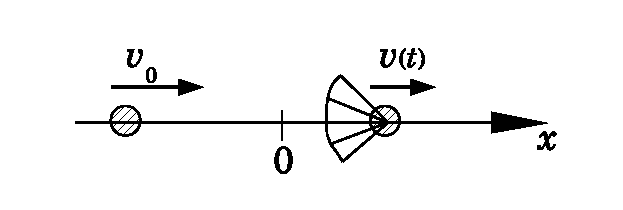
\includegraphics[width=7cm]{parachute.eps}
    \caption{等速直線運動している物体に突然空気抵抗がかかる。}\label{fig:parachute}
\end{figure}
\begin{enumerate}
\item $t<0$では, 次式が成り立つことを示せ:
\begin{eqnarray}
0=m\frac{dv}{dt}\label{eq:friction_stop1}
\end{eqnarray}
\item $0<t$では, 次式が成り立つことを示せ:
\begin{eqnarray}
-\alpha v=m\frac{dv}{dt}\label{eq:friction_stop2}
\end{eqnarray}
\item 上の式は, 関数$v(t)$に関する微分方程式だ。数学の教科書
を参考にして, この微分方程式を解け。結果は次式のようになるはずである:
\begin{eqnarray}
v(t)=v_0\exp\Bigl(-\frac{\alpha}{m}t\Bigr)\label{eq:stop_viscosity}
\end{eqnarray}
\item 関数$v(t)$のグラフを描け。
\end{enumerate}
\end{q}

このように, 空気や水などの流体\footnote{気体と液体をまとめて流体と呼ぶ。}の中で物体が速度に比例して受ける抵抗を\underline{粘性抵抗}
\index{ねんせいていこう@粘性抵抗}という。
しかしながら, 物体が大きかったり速度が速いとき, 速度の2乗に比例する
抵抗をより強く受ける。それを\underline{慣性抵抗}\index{かんせいていこう@慣性抵抗}という
\footnote{このあたりの法則は, 流体力学という物理学で説明されるが, 流体力学のほとんど
はニュートン力学を基本法則とする。}。\mv

%
\begin{q}\label{q:resistance}
粘性抵抗とは何か? 慣性抵抗とは何か?
\end{q}

%
\begin{q}\label{q:parachute2}
問\ref{q:parachute}において, パラシュートによる空気抵抗が粘性抵抗でなく慣性抵抗ならどうなるだろう? 
いま, 空気抵抗が$-\beta v^2$であるとする($\beta $は適当な定数)。
\begin{enumerate}
\item パラシュートが開いてから物体が停止するまでの間, 次式が成り立つことを示せ:
\begin{eqnarray}
-\beta\,v^2=m\frac{dv}{dt}\label{eq:parachute20}
\end{eqnarray}
\item 上の微分方程式を変数分離すると, 次式のようになることを示せ:
\begin{eqnarray}
\beta\,dt=-\frac{mdv}{v^2}\label{eq:parachute21}
\end{eqnarray}
\item これを不定積分すると, 次式のようになることを示せ($C$は積分定数):
\begin{eqnarray}
\beta\,t=\frac{m}{v}+C\label{eq:parachute22}
\end{eqnarray}
\item 以下の式が成り立つことを示せ。
\begin{eqnarray}
C=-\frac{m}{v_0}\label{eq:parachute23}
\end{eqnarray}
\item 以下の式が成り立つことを示せ。
\begin{eqnarray}
v(t)=\frac{mv_0}{v_0\,\beta\,t+m}\label{eq:parachute24}
\end{eqnarray}
\item 関数$v(t)$のグラフを描け:
\end{enumerate}
\end{q}
\mv

\begin{faq}{\small\textgt{問\ref{q:parachute}で, 
なぜ最初は力0なのですか? 力がないと進まないのでは? } ... 
物体は, \textgt{力がなくても動き続ける}のです。
等速直線運動をするのです。それが慣性の法則です。
「力がないと物体は進まない」というのは間違いです。
思い込みです。止まっている物体を動き出させる
ためには, 確かに最初に力をかけてやる必要がありますが, いったん動き出せば, 
力をかけなくても物体は勝手に動き続けるのです。}\end{faq}\mv

\begin{faq}{\small\textgt{物体が力を受けなくても等速で
動くのなら止まっている物体は力を受けて止まっているのですか?} ... 
いいえ。「止まっている」も「等速で動く」ことの一種で, 働く力は0です。}\end{faq}\mv

%
\begin{q}\label{q:raindrop}
雨粒の落下を考えよう。雨粒は重力を受けて加速しながら落下するが, 同時に空気抵抗も受けるので, 
際限なく加速することはあり得ない。また, 雨粒が十分小さければ, 空気抵抗は粘性抵抗とみなすことができる。
いま, 鉛直上向きに座標軸をとる。質量$m$の雨粒が鉛直方向に直線的に落下するとし, 時刻$t$における雨粒
の落下速度を$v(t)$とする。$v(0)=0$とする。雨粒にかかる空気抵抗(粘性抵抗)を$-\alpha v$とする
($\alpha$は適当な正の定数)。注:落下は下向きだから$v$は負であり, 空気抵抗"$-\alpha v$"は$v$にマイナスが
かかっているから正, つまり上向きである。
\begin{enumerate}
\item 雨粒に関する運動方程式は以下のようになることを示せ:
\begin{eqnarray}
-mg-\alpha v=m\frac{dv}{dt}\label{eq:raindrop1}
\end{eqnarray}
\item これを変数分離すると次式になることを示せ:
\begin{eqnarray}
\frac{dv}{g+\alpha v/m}=-dt\label{eq:raindrop2}
\end{eqnarray}
\item これを両辺を積分すると次式になることを示せ($C$は積分定数):
\begin{eqnarray}
\frac{m}{\alpha}\ln\Bigl|v+\frac{gm}{\alpha}\Bigr|=-t+C\label{eq:raindrop3}
\end{eqnarray}
\item これを$v$について解き, 特に$v(0)=0$に注意して, 次式を示せ:
\begin{eqnarray}
v(t)=\frac{mg}{\alpha}\Bigl\{\exp\Bigl(-\frac{\alpha}{m}t\Bigr)-1\Bigr\}\label{eq:raindrop4}
\end{eqnarray}
\item $v(t)$のグラフを描け。
\item 時間が十分にたって速度が一定になったときの速度を\underline{終端速度}
\index{しゅうたんそくど@終端速度}という。この場合, 終端速度は
\begin{eqnarray}v=-\frac{mg}{\alpha}\end{eqnarray}
となることを示せ。
\end {enumerate}
\end{q}
\mv

雨が降る時, 雨粒は地表面に衝撃を与える。地表を植生が覆っていれば, 
葉やリター(落ち葉等)で雨滴衝撃を吸収してくれるが, 地表に植生が無い
場合は, 雨滴衝撃で土壌侵食を起こすことがある。これは農地や, 間伐が不十分
なスギ・ヒノキ人工林などで問題になっている。\mv

粘性抵抗を受ける落下の問題は, 微粒子(穀物の粉とか, 大気汚染源の粉塵など)の運動を議論する上で
基礎的なものだ。また, 微粒子の大きさを計測する上でもこの理論がよく利用される。

\begin{comment}
では, 慣性抵抗を受ける落下運動はどうなるだろう?
\mv
\begin{figure}[h]
    \centering
    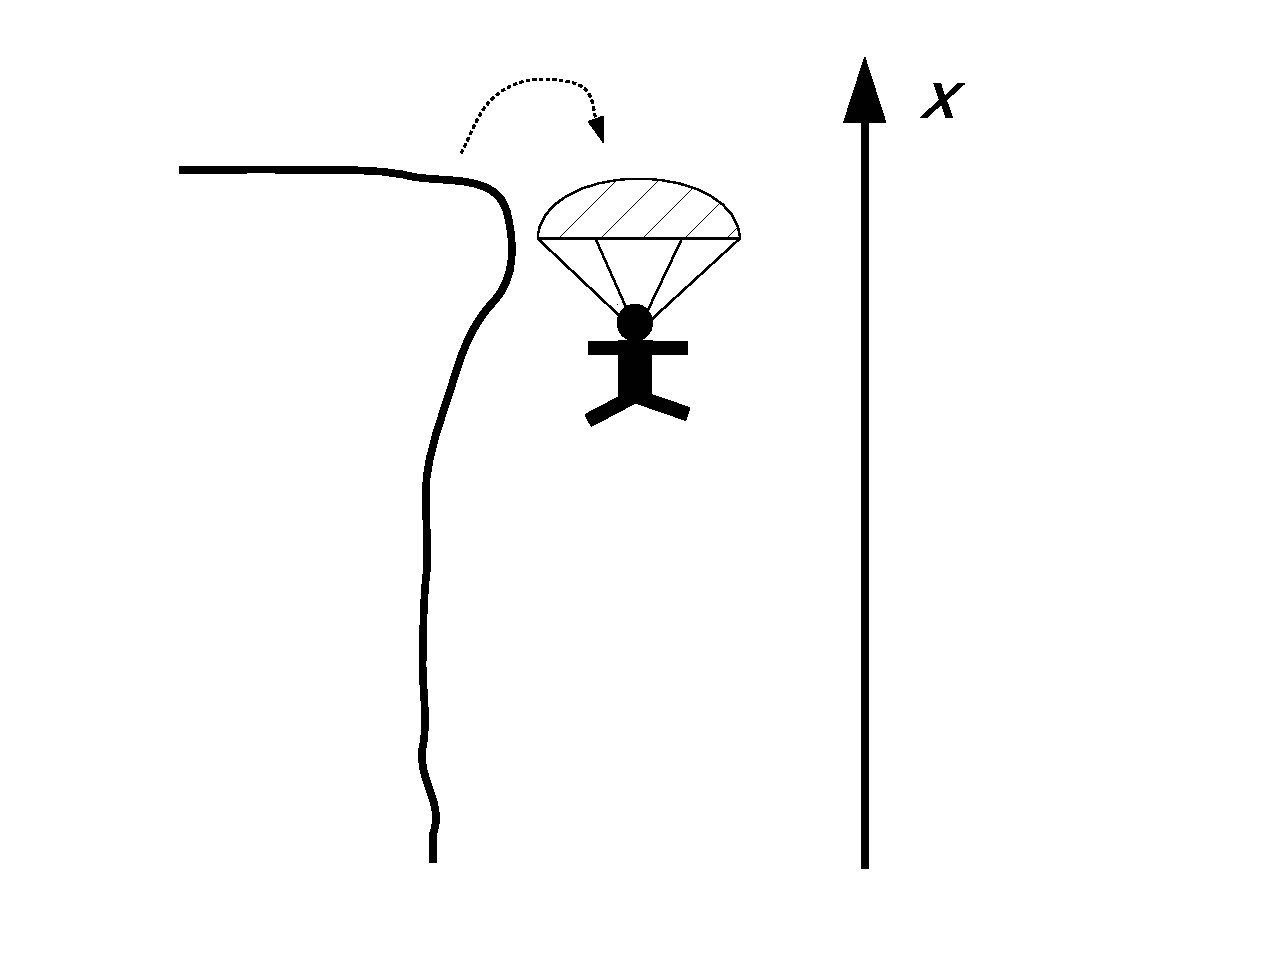
\includegraphics[width=5cm]{cliff_fall.eps}
    \caption{崖からパラシュートで降下する。詳しくは問\ref{q:parachute_energy}参照。}\label{fig:cliff_fall}
\end{figure}

\begin{q}\label{q:parachute_energy}
君は高い崖の上からパラシュートで降下しようとしている(図\ref{fig:cliff_fall})。
君は重力を受けて加速しながら落下するが, 
同時に空気抵抗も受けるので, 際限なく加速することはあり得ない。また, このような場合, 君が受ける空気抵抗は
慣性抵抗とみなすことができる。いま, 鉛直上向きに座標軸をとる。質量$m$の君が鉛直方向に直線的に落下
するとし, 時刻$t$における君の落下速度を$v(t)$とする。君にかかる空気抵抗(慣性抵抗)を$\beta v^2$とする
($\beta$は適当な正の定数)。
注:落下は下向きだが, 空気抵抗は上向き, つまり空気抵抗の符号は正である。
\begin{enumerate}
\item 君に関する運動方程式は以下のようになることを示せ:
\begin{eqnarray} 
-mg+\beta v^2=m\frac{dv}{dt}\label{eq:parachute_fall1}
\end{eqnarray} 
\item 時間が十分にたつと, 空気抵抗と重力がつりあって, 速度は一定値になるはずだ。そのとき, 
上の式で$dv/dt=0$となる。それを利用して, 終端速度の大きさ$v_{\infty}$は, 
\begin{eqnarray}v_{\infty}=\sqrt{\frac{mg}{\beta}}\end{eqnarray}
となることを示せ。(ただし, もし向きまで考えるならばこの式にマイナスが付く。ここでは向きは考えず, 大きさだけを考えている。)
\item $v_{\infty}$を使うと, 上の方程式は次式のように書き換えることができることを示せ:
\begin{eqnarray}m\frac{dv}{dt}=\beta (v^2-v_{\infty}^2)\end{eqnarray}
\item これを変数分離して部分分数展開(数学リメディアル教材参照)すると, 次式になることを示せ:
\begin{eqnarray}\Bigl(\frac{1}{v-v_{\infty}}-\frac{1}{v+v_{\infty}}\Bigr)\frac{dv}{2v_{\infty}}=\frac{\beta}{m}dt\end{eqnarray}
\item 両辺積分すると次式になることを示せ(ここで$C$は積分定数)
\begin{eqnarray}\frac{1}{2v_{\infty}}\ln\Bigl|\frac{v-v_{\infty}}{v+v_{\infty}}\Bigr|=\frac{\beta}{m}t+C\label{eq:parachute_fall5}
\end{eqnarray}
\item 初速度$v(0)$を0とすると, 次式のようになることを示し, $v(t)$のグラフを描け。
\begin{eqnarray}v=-v_{\infty}\tanh\Bigl(v_{\infty}\frac{\beta}{m}t\Bigr)\end{eqnarray}
ただし, $\tanh x$は「双曲線関数」と呼ばれる関数の一種であり, その定義は, 
\begin{eqnarray}\tanh x=\frac{e^x-e^{-x}}{e^x+e^{-x}}\end{eqnarray}
である。$\tanh$を「ハイパボリック・タンジェント」と呼ぶ。
\end{enumerate}
\end{q}
\mv
\end{comment}


\section{運動の三法則と哲学}

本章の最後に, ちょっと哲学っぽいことを考えよう。運動の三法則は, 
物体の運動を正確に予測することができる, ということを世界に示した。
それは, 未来を占うのにオカルト的な力が必要だと信じていた人に, 
ちょっとしたショックを与えただろう。そこで生まれたのが
「ラプラスの悪魔」という概念である。\mv

\begin{q}\label{q:Laplace_demon}
「ラプラスの悪魔」とは何か? それは近代の宗教や思想にどのような影響を与えただろうか? 
それは物理学的にはどのように反駁(はんばく)されたか? 
\end{q}
\hv
\begin{comment}
\begin{q}\label{q:cheat_experiment}
ある高校には, 地元の有名な学習塾に通う生徒が大勢いた。彼らは学校の理科の
実験で, 配られた記録用紙に塾で習った実験結果を手早く書き, 余った時間を
テスト対策の内職勉強をしていた。彼らは, 結果がわかりきった実験をわざわざ
繰り返す必要は無いし, 時間の無駄であるという。彼らの行為や考え方について
自由に論じよ。\end{q}
\hv
\end{comment}

\begin{exq} 質量$m$の質点に, $x$軸の正の方向に$F=Ae^{-kt}$という力がかかっている。
ここで, $A, k$は正の定数であり, $t$は時刻。質点の速度$v$を$t$の関数として
表せ。ただし初速度を0とする。\end{exq}

\begin{exq} 2つの質点A, Bが, 質量を持たないバネでつながれている。質点Aを水平方向にひっぱる
ことで, これらを摩擦の無い水平面上で, 加速度0.50~m~s$^{-2}$で等加速度直線運動をさせる。質点A, Bの
質量はそれぞれ2.0~kgと3.0~kgとし, バネ定数は4.5~N/mとする。バネの伸びを求めよ。
ヒント: 2つの質点のそれぞれについて運動方程式を立てる。\end{exq}

\begin{exq} ジャンボジェット機(ボーイングB747)が, 成田空港の, 
幅60~mの滑走路に, その中心線を目指ざして着陸しようとしている。あと5秒で
車輪が滑走路につくというとき, 突然, 横から$v=10$~m/sの突風が吹いてきた。この飛行機は
無事に滑走路内に着陸できるか? 根拠と共に示せ。ただし, 物体が風から受ける力
(慣性抵抗)の大きさ$F$は, $F=\rho v^2 S C_{\text{D}}/2$と表せることが知られている。
ここで$\rho$は空気の密度であり, $S$は風の方向に投影した物体の面積である。$C_{\text{D}}$は「抗力係数」
と呼ばれる無次元の数で, 物体の形状や風の性質に依存するが, おおよそ0.5から2程度の値
である。また, ジャンボジェットの質量は乗客も含めて約300~t, ジャンボ・ジェットの
胴体は全長70~m, 直径8~m程度である。\end{exq}




\section{解答}

\noindent{\textbf{答}}\ref{q:motion1condition}
(1) AはCの十分条件。必要条件ではない。静止していれば合力はゼロだが, 
合力がゼロであっても静止していない場合(${\bf 0}$以外の速度での等速直線運動)があり得る。
(2) BはCの必要十分条件。
(3) BはAの必要条件。十分条件ではない。静止は等速直線運動の一種(速度${\bf 0}$での等速直線運動)。
\mv

%\noindent{\textbf{答}}\ref{q:escalator} 略。ヒント: 
%エスカレーターが突然停止したらどうなるか?\mv

% 運動の三法則とは何か? 
%\noindent{\textbf{答}}\ref{q:Newton_3laws} 略。
%\vspace{0.2cm}

\noindent{\textbf{答}}\ref{q:NewtonLaw_mistake} 
(1) 間違い。「AはBから, 同じ\textgt{大きさで逆向きの}力を受ける」
(2) 正しい。質点が等速直線運動をしているとき, 加速度${\bf a}$は${\bf 0}$である。
従って, 第二法則より, 物体にかかる合力${\bf F}$は${\bf 0}$である。
(3) 直線方向の運動(1次元の運動)に限定すれば正しい。しかし一般には, 
力も加速度もベクトルなので, $F$と$a$のかわりに${\bf F}$と${\bf a}$と
書かねばならない。
\mv

% 運動量とは何か? 
%\noindent{\textbf{答}}\ref{q:def_momentum} 質量($m$)と速度(${\bf v}$)の積$m{\bf v}$。
%\vspace{0.2cm}

% 地表付近で重力だけを受けて上下運動をする, 
\noindent{\textbf{答}}\ref{q:freefall0}
\begin{enumerate}
\item \eref{eq:gravity_earth}より, 質点には鉛直下向きに大きさ$mg$の重力がかかる。
座標系は鉛直上向きを正にとっているので, この重力$F$は$F=-mg$
と書ける\footnote{\eref{eq:gravity_earth}は力の向きは考えず力の大きさだけを
考えていたことに注意せよ。}。重力以外の力は働いていない。従って運動方程式より, 
$-mg=ma$
\item \eref{eq:constacc_vx}, \eref{eq:constacc_x}で, $a_x$を$-g$, $v_x$を$v$とすれば, 与式を得る。
\item $x_0=0$, $v_0=0$とすればよい。
\end{enumerate}
\mv


% 地表付近で, 初速度0で質点を投下し, 自由落
\noindent{\textbf{答}}\ref{q:freefall1} 初期位置を原点とし, 鉛直上向きに$x$軸をとる。時刻$t$における位置と速度をそれぞれ$x(t)$, $v(t)$とする。
(1) \eref{eq:freefallveq0}, \eref{eq:freefallxeq0}で$t=10$~sとすれば, $v=-98$~m~s$^{-1}$, $x=-490$~m。従って落下距離は490~m。
(2) 加速度が$-g$の等加速度直線運動なので$v(t)=-gt$。従って$t=-v(t)/g$。
いま, $v(t)=-340$~m~s$^{-1}$なので, $t=340$~m~s$^{-1}$/(9.8~m~s$^{-2}$) =35~s。従って約35秒後。
\eref{eq:freefallxeq0}で$t=35$~sとすれば, $x=-6000$~m。従って, 約6000~m落下する。
\vspace{0.2cm}

% プロ野球投手が初速度$v_0=40$m/s(約140km/hに相当)でボ
\noindent{\textbf{答}}\ref{q:baseball0}\\
\eref{eq:freefallxeq}で, $x_0=0$とすれば, 
\begin{eqnarray}
x(t)&=&v_0t-\frac{1}{2}gt^2=-\frac{1}{2}g\Bigl(t^2-\frac{2v_0}{g}t\Bigr)\\
    &=&-\frac{1}{2}g\Bigl(t-\frac{v_0}{g}\Bigr)^2+\frac{v_0^2}{2g}
\end{eqnarray}
従って, $t=v_0/g$のとき, 最高高度$v_0^2/(2g)$に到達する。ここで$v_0=40$~m~s$^{-1}$とすると, 最高高度は, 
\begin{eqnarray}
\frac{(40\text{ m s}^{-1})^2}{2\times9.8\text{ m s}^{-2}} =82\text{ m}
\end{eqnarray}
すなわち, 約80~mの高さまで届く。
(グラフは省略。)
\vspace{0.2cm}

% カーリングというスポーツでは, 氷の上で石(ストーン)を滑らせて当てあう
\noindent{\textbf{答}}\ref{q:curling}
\begin{enumerate}
\item 手放された後のストーンに働く力は, 氷面からうける
動摩擦力$F_{\text m}$と, 重力である。重力は氷面から受ける垂直抗力と打ち消し合う。また, 摩擦力$F_{\text m}$は
$x$軸の逆方向に働く。従って, ストーンに働く力の総和$F$は, $F=-F_{\text m}$となる。加速度を$a$とすると, 
運動方程式は, 
\begin{eqnarray}
-F_{\text m}=ma
\end{eqnarray}
\item 前小問より, $a=-F_{\text m}/m$となるが, これは時刻によらない一定値。
すなわちこれは等加速度直線運動である。
\eref{eq:constacc_vx}, \eref{eq:constacc_x}で, $a_x$を$-F_{\text m}/m$, 
速度$v_x$を$v$とすれば, 
\begin{eqnarray}
v&=&v_0-\frac{F_{\text m}}{m}\,t\label{eq:stonev}\\
x&=&v_0t-\frac{F_{\text m}}{2m}\,t^2\label{eq:stonex}
\end{eqnarray}
となる。ここで$x(0)=0$, $v(0)=v_0$を用いた。グラフは図\ref{fig:stone}のようになる。
\begin{figure}[h]
    \centering
    \includegraphics[width=4cm]{stone.eps}
    \caption{カーリングのストーンの運動。}\label{fig:stone}
\end{figure}
\item ストーンが停止した時刻を$t$, そのときの位置を$x$とすると, 
そのとき速度$dx/dt$は0になるから, 
式(\ref{eq:stonev})より, 
\begin{eqnarray}
0=-\frac{F_{\text m}}{m}\,t+v_0
\end{eqnarray}
従って, $t=mv_0/F_{\text m}$。これを式(\ref{eq:stonex})に代入すると, 
\begin{eqnarray}
x=\frac{mv_0^2}{2F_{\text m}}\label{eq:stonexx}
\end{eqnarray}
従って, 
\begin{eqnarray}
F_{\text m}=\frac{mv_0^2}{2x}\label{eq:stoneFm}
\end{eqnarray}
ここで, $x=20$~m, $m=20$~kg, $v_0=1.5$~m~s$^{-1}$とすれば, $F_{\text m}=1.1$ N。
\item クーロンの摩擦法則(式(\ref{eq:friction_m}))より, 動摩擦係数$\mu'$について, 
\begin{eqnarray}
F_{\text m}=\mu' N\label{eq:curling_Fm}
\end{eqnarray}
が成り立つ。ここで$N$はストーンと氷の接触面に垂直に働く力であり, 今の場合は$N=mg$である。従って, 
$F_{\text m}=\mu' mg$である。従って, 上の結果から, 
$\mu'=F_{\text m}/(mg)=5.7\times10^{-3}$。(無次元
なので単位は不要)
\item 式(\ref{eq:stonexx})より, 停止するまでの距離$x$は, 初速度$v_0$の2乗に比例する。
$x$を20~mから25~mにするとき, $x$は1.25倍になるが, そのためには$v_0$が$\sqrt{1.25}=1.12$倍
になればよい。従って, $v_0$は$\sqrt{1.25}\times1.5$~m~s$^{-1}$=1.68~m~s$^{-1}$。つまり, 約1.7~m~s$^{-1}$にすればよい。
\item \eref{eq:stonexx}と\eref{eq:curling_Fm}で$F_{\text m}$を消去し, $F_{\text m}=\mu' mg$を使えば, 
\begin{eqnarray}
x=\frac{v_0^2}{2\mu'g}\label{eq:stonexx2}
\end{eqnarray}
となる。従って$x$は質量に依存しない。従って, 30~kgだろうが何kgだろうが, 
摩擦の条件(氷の表面状態とストーンの底面材質)が同じなら, 前小問で
求めた初速度(約1.7~m~s$^{-1}$)でよい。
\end{enumerate}
\vspace{0.2cm}

\begin{faq}{\small\textgt{問\ref{q:curling}(6)に驚きました。
重い物体が, 軽い物体と同じ初速度で同じ距離で止まるのですか?}
... そうです。不思議ですね。これは, 力が摩擦力だからです。この場合の
摩擦力は, 重力に比例します。重い物体にはそのぶん, 垂直効力が
大きくなるため, 大きな摩擦力がかかるのです。つまり$F=ma$の左辺の$F$が$m$に比例するため, 
右辺の$ma$の$m$と打ち消し合って, 結果的に質量の影響は
無くなるのです。}\end{faq}\mv


\noindent{\textbf{答}}\ref{q:increase_force} 
質量を$m$, 時刻を$t$, 力を$F(t)$とする。力は時刻に比例するので, 
\begin{eqnarray}
F(t)=bt\label{eq:increase_force}
\end{eqnarray}
と書ける($b$は適当な定数)。運動方向に$x$軸をとり, 
位置を$x(t)$, 速度を$v(t)$, 加速度を$a(t)$とする。運動方程式より, $F(t)=ma(t)$。
これに\eref{eq:increase_force}を代入して変形すると,
\begin{eqnarray}
a(t)=\frac{bt}{m}\label{eq:increase_force2}
\end{eqnarray}
となる。\eref{eq:vxfromax}のように考えて($a_x$, $v_x$はここでは$a$, $v$), 
\begin{eqnarray}
v(t)&=&v(0)+\int_{0}^{t}a(t)\, dt\label{eq:increase_force3}
\end{eqnarray}
である。ここで$v(0)=0$と, \eref{eq:increase_force2}を代入して, 
\begin{eqnarray}
v(t)&=&\int_{0}^{t}\frac{bt}{m}\, dt=\frac{bt^2}{2m}\label{eq:increase_force4}
\end{eqnarray}
また, \eref{eq:xfromvx}のように考えて, 
\begin{eqnarray}
x(t)&=&x(0)+\int_{0}^{t}v(t)\, dt
\end{eqnarray}
である。ここで$x(0)=0$と, \eref{eq:increase_force4}を代入して, 
\begin{eqnarray}
x(t)&=&\int_{0}^{t}\frac{bt^2}{2m}\, dt=\frac{bt^3}{6m}\label{eq:increase_force6}
\end{eqnarray}
さて, \eref{eq:increase_force}で$t=$2.0~sのときを考えると, 
6.0~N$=b\times$2.0~sだから, $b=3.0$~N/s。これと, $m$=2.0~kg, $t=$4.0~sを
\eref{eq:increase_force6}に代入すると, 
\begin{eqnarray}
x(4.0\text{ s})&=&\frac{(3.0\text{ N/s})(4.0\text{ s})^3}{6\times 2.0\text{ kg}}=16\text{ m}
\end{eqnarray}
\mv

% 質量$m$の物体が, 速度$v_0$で等速直線運動している
\noindent{\textbf{答}}\ref{q:parachute}
\begin{enumerate}
\item $t<0$では等速直線運動をしているから, 慣性の法則より, 働く力(の総和)は0である。
従って, 運動方程式より, 式(\ref{eq:friction_stop1})が成り立つ。
\item $0<t$ではパラシュートによる空気抵抗力$F=-\alpha v$がかかる。従って, 運動方程式より, 式(\ref{eq:friction_stop2})が成り立つ。
\item 式(\ref{eq:friction_stop2})を変数分離すると, 
\begin{eqnarray}-\alpha dt=m\frac{dv}{v}\end{eqnarray}
さて, 上の式を両辺, 積分すると($C$は積分定数), 
\begin{eqnarray}-\alpha t=m\ln|v|+C\end{eqnarray}
($C'$は$C$とは別の定数)。従って, 
\begin{eqnarray}v=\pm \exp\Bigl(-\frac{\alpha}{m}t+C'\Bigr)=\pm C'\,\exp\Bigl(-\frac{\alpha}{m}t\Bigr)\quad\quad\quad\end{eqnarray}
ここで$t=0$のとき$v=v_0$だから, 
\begin{eqnarray}\pm \exp C'=v_0\end{eqnarray}
従って, 
\begin{eqnarray}v=v_0 \exp\Bigl(-\frac{\alpha}{m}t\Bigr)\end{eqnarray}
\item 図\ref{fig:viscos}のようになる。
\begin{figure}[h]
    \centering
    \includegraphics[width=7cm]{viscos.eps}
    \caption{粘性抵抗を受けて減速する物体の運動。}\label{fig:viscos}
\end{figure}
\end{enumerate}
\vspace{0.2cm}

% 粘性抵抗とは何か? 慣性抵抗とは何か?
%\noindent{\textbf{答}}\ref{q:resistance}\\
%粘性抵抗とは, 流体の中で, 物体が速度に比例して受ける抵抗力。慣性抵抗とは, 物体が流体の中で速度の二乗
%に比例して受ける抵抗力。
%\vspace{0.2cm}

% 前問において, パラシュートによる空気抵抗が粘性抵抗でなく慣性抵抗な
\noindent{\textbf{答}}\ref{q:parachute2}
(1) $0<t$ではパラシュートによる空気抵抗力$F=-\beta v^2$がかかる。従って, 運動方程式より, \eref{eq:parachute20}が成り立つ。
(2), (3) 略。
(4) \eref{eq:parachute22}で, $t=0$とすれば, $0=m/v(0)+C$。従って$C=-m/v(0)$。
(5) \eref{eq:parachute23}を\eref{eq:parachute22}に入れて$v$についてとけば, 
\eref{eq:parachute24}が成り立つ。(各自, 計算してみよ) 
(6) 図\ref{fig:inert_v}のようになる。
\begin{figure}[h]
    \centering
    \includegraphics[width=7cm]{inert_v.eps}
    \caption{慣性抵抗を受けて減速する物体の運動。}\label{fig:inert_v}
\end{figure}
\vspace{0.2cm}


% 雨粒の落下を考えよう。雨粒は重力を受け
\noindent{\textbf{答}}\ref{q:raindrop}
\begin{enumerate}
\item 雨粒にかかる力は, 重力($-mg$)と粘性抵抗($-\alpha v$)の和。
従って, 運動方程式より, \eref{eq:raindrop1}が成り立つ。
\item \eref{eq:raindrop1}の両辺を$m$で割ると, 
\begin{eqnarray}-g-\frac{\alpha v}{m}=\frac{dv}{dt}\end{eqnarray}
両辺に$dt$をかけ, さらに両辺を$g+\alpha v/m$で割ると, 
\begin{eqnarray}-dt=\frac{dv}{g+\alpha v/m}\end{eqnarray}
この左辺と右辺を入れ替えると, \eref{eq:raindrop2}を得る。
\item \eref{eq:raindrop2}の両辺に積分記号$\int$をつける:
\begin{eqnarray}\int\frac{dv}{g+\alpha v/m}=-\int dt\end{eqnarray}
この左辺の不定積分は, 
\begin{eqnarray*}
\int\frac{dv}{(\alpha/m)(v+gm/\alpha)}=\frac{m}{\alpha}\int\frac{dv}{v+gm/\alpha}\\
=\frac{m}{\alpha}\ln\Bigr|v+\frac{gm}{\alpha}\Bigl|+C_1
\end{eqnarray*}
となる($C_1$は積分定数)。右辺の不定積分は, $-t+C_2$となる($C_2$は積分定数)。これらをまとめて, 
\begin{eqnarray}
\frac{m}{\alpha}\ln\Bigl|v+\frac{gm}{\alpha}\Bigr|+C_1=-t+C_2
\end{eqnarray}
となる。$C_1$を右辺に移項し, $C_2-C_1=C$とおけば, \eref{eq:raindrop3}を得る。
\item \eref{eq:raindrop3}より, 
\begin{eqnarray}
\ln\Bigr|v+\frac{gm}{\alpha}\Bigl|=-\frac{\alpha}{m}(t-C)
\end{eqnarray}
従って, 
\begin{eqnarray}
v+\frac{gm}{\alpha}=\pm\exp\Bigl[-\frac{\alpha}{m}(t-C)\Bigr]
\end{eqnarray}
従って, 
\begin{eqnarray}
v=\pm\exp\Bigl[-\frac{\alpha}{m}(t-C)\Bigr]-\frac{gm}{\alpha}\label{eq:randrop_ans11}
\end{eqnarray}
ここで$t=0$, $v=0$とおけば, 
\begin{eqnarray}
0=\pm\exp\Bigl[\frac{\alpha}{m}C\Bigr]-\frac{gm}{\alpha}
\end{eqnarray}
従って, 
\begin{eqnarray}
\pm\exp\Bigl[\frac{\alpha}{m}C\Bigr]=\frac{gm}{\alpha}
\end{eqnarray}
となる(左辺の$\pm$も含めて右辺のように決まる)。これを\eref{eq:randrop_ans11}に代入して, 
\begin{eqnarray}
v=\frac{gm}{\alpha}\exp\Bigl[-\frac{\alpha}{m}\,t\Bigr]-\frac{gm}{\alpha}
\end{eqnarray}
これを整理すると\eref{eq:raindrop4}を得る。
\item 図\ref{fig:viscos_fall}のようになる。
\begin{figure}[h]
    \centering
    \includegraphics[width=7cm]{viscos_fall.eps}
    \caption{粘性抵抗を受ける落下。}\label{fig:viscos_fall}
\end{figure}
\item \eref{eq:raindrop4}において$t$の$\infty$への極限で, $v$は$-mg/\alpha$に近づく。
あるいは, 終端速度では速度は時間とともに変わらないから, \eref{eq:raindrop1}の右辺を
0とおけば, 同じく$v=-mg/\alpha$を得る。
\end{enumerate}
\vspace{0.2cm}

\begin{comment}
% 君は高い崖の上からパラシュートで降下しようとしている
\noindent{\textbf{答}}\ref{q:parachute_energy}
\begin{enumerate}
\item 君にかかる力は, 重力($-mg$)と空気抵抗力($\beta v^2$)の合力である。
そこで, 
\begin{eqnarray}F=-mg+\beta v^2\end{eqnarray}
として, 1次元の運動方程式$F=mdv/dt$に代入すれば, 与式を得る。
\item $v$の大きさが一定値$v_\infty$に至ったとして, $dv/dt=0$とすれば, 式(\ref{eq:parachute_fall1})より, $-mg+\beta v^2=0$。
従って, このとき, $|v|=\sqrt{mg/\beta}=v_\infty$。
\item 略($v_\infty$を使って式(\ref{eq:parachute_fall1})から$g$を消せばよい)。
\item 略。
\item 略。
\item \eref{eq:parachute_fall5}より, 
\begin{eqnarray}
\frac{v-v_\infty}{v+v_\infty}=\pm\exp\Bigl(2v_\infty\bigl(\frac{\beta}{m}\,t+C\bigr)\Bigr)
\end{eqnarray}
これに, $t=0$, $v=0$を代入して左辺=右辺となるようにするには, 右辺の符号はマイナスであり, かつ, $C=0$とするしかない。従って, 
\begin{eqnarray}
\frac{v-v_\infty}{v+v_\infty}=-\exp\Bigl(2v_\infty\frac{\beta}{m}\,t\Bigr)
\end{eqnarray}
これを$v$について解けば(詳細略), 次式のようになる:
\begin{eqnarray}
v=-v_\infty\frac{\exp\Bigl(2v_\infty\frac{\beta}{m}\,t\Bigr)-1}{\exp\Bigl(2v_\infty\frac{\beta}{m}t\Bigr)+1}
\end{eqnarray}
右辺の分子と分母にそれぞれ
\begin{eqnarray}
\exp\Bigl(-v_\infty\frac{\beta}{m}\,t\Bigr)
\end{eqnarray}
をかければ, 
\begin{eqnarray*}
v=-v_\infty\frac{\exp\Bigl(v_\infty\frac{\beta}{m}\,t\Bigr)-\exp\Bigl(-v_\infty\frac{\beta}{m}\,t\Bigr)}{\exp\Bigl(v_\infty\frac{\beta}{m}\,t\Bigr)+\exp\Bigl(-v_\infty\frac{\beta}{m}\,t\Bigr)}
\end{eqnarray*}
となる。この右辺は, 
\begin{eqnarray}
-v_\infty\tanh\Bigl(v_\infty\frac{\beta}{m}\,t\Bigr)
\end{eqnarray}
である。グラフは図\ref{fig:inert_fall}のとおり:
\begin{figure}[h]
    \centering
    \includegraphics[width=7cm]{inert_fall.eps}
    \caption{慣性抵抗を受ける落下。}\label{fig:inert_fall}
\end{figure}
\end{enumerate}
\end{comment}

%
\noindent{\textbf{答}}\ref{q:Laplace_demon}\\
略(各自, 調べよ)。
\hv


\begin{faq}{\small\textgt{摩擦のない面に10~tくらいの
物体がのって静止しているとします。摩擦がなければ, この物体を
面と平行な方向に動かし始めるには, ほんの少し力をかけて
やるだけで良いのでしょうか。イメージできない。} ... 
はいそうです。実際, 小惑星探査機「はやぶさ」は
500~kgほどですが, それを動かすイオンエンジンは1円玉
を持ち上げるくらいの力しかなかったらしいですよ。}\end{faq}

\begin{comment}
\begin{faq}{\small\textgt{ラプラスの悪魔にびっくりしました。} ... 
私も若い頃, ラプラスの悪魔を知って, 自分の人生は
もう決まってるのかと, 一瞬, 凹みました。}\end{faq}

\begin{faq}{\small\textgt{解答をみるとわかるんですけど, 
一から自分で解答を作り出せません。} ... 基本から丁寧に
理解することが重要で, 必ずしも「一から作り出す」ことには
こだわらなくていいです。受験勉強じゃないんだし, 
新しいことを学んでいるのだから。}\end{faq}\mv
\end{comment}


\chapter{さまざまな運動}

注: この章を理解するには, 数学リメディアル教材で三角関数を理解していることが必要である。\mv

\section{単振動}\index{たんしんどう@単振動}
\begin{figure}[h]
    \centering
    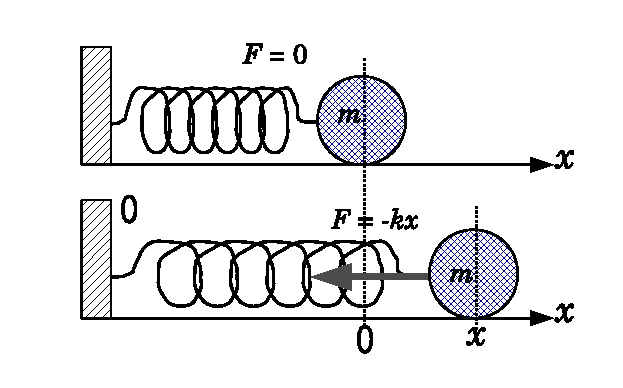
\includegraphics[width=7cm]{spring_vib.eps}
    \caption{バネにつけられて振動する物体}\label{fig:spring_vib}
\end{figure}

図\ref{fig:spring_vib}のように, 壁に一端が固定されたバネの, もう一端に質量$m$の物体がとりつけられた
系を考えよう。物体と床面の間に摩擦は無いものとする。バネ定数を$k$とし, バネ自体の質量は無視する。
バネはこの図の左右方向にのみ伸び縮みし, 物体もこの図の左右方向にしか動かないとする。バネが自然長
にあるときの物体の位置を原点とし, 左右方向に沿って$x$軸をとる。バネの伸びる方向を$x$軸の正の方向
とする。

%2011.4.3 ヤマサキ (4章で摩擦のない/ある運動を考えてるのでややくどいけど万全を期して)摩擦は考えないことを強調する脚注をつけました
この物体を, 右か左から指で弾いたり, 右か左に少し動かして放すと, 
物体は左右に振動しはじめることは, 君の日常経験から明らかだろう。
ただし, 日常経験だけで考えると, この振動運動はいつか止まって
しまうように思われる。しかし, ここでは「物体と床面の間に摩擦は無い」
と仮定しているので, 他に何らかの外力が働かない限り, 
この振動運動は永遠に続く。この運動を物理的に考えよう。

物体の運動を考えるときは, いつでも運動方程式(\ref{eq:motion})から出発する。
運動方程式は, 質量$m$が一定であれば, 力のベクトルと加速度のベクトルの関係式だ。
従って, 運動方程式を考えるということは, $x$方向, $y$方向, $z$方向
の各方向について, 力と加速度の関係を考えるということだ。

ところが, いま考えている物体は左右方向しか動かないので, 上下方向や
奥行き方向について運動方程式を考える必要は無い\footnote{とは言うものの, 
念のため, 上下方向の運動も考えておこう: 物体に上下方向(鉛直方向)に働く力は, 
重力(下向き)と, 床からの垂直抗力(上向き)だ。これらは同じ大きさで逆向き
だから互いに打ち消しあう。従って, 物体に働く上下方向の力(合力)は0だ。
従って, 物体が最初に床にあって上下方向に運動していない限り, 慣性の法則に
従って, 物体は床(高さ0)にあり続ける。従って上下方向の加速度は0だ。
従って, 上下方向の運動方程式は, $0=0$となるにすぎない。}。
そこで, 左右方向の運動方程式だけを考える: いま, バネが自然長にある
(伸びも縮みもない状態)では, バネが物体に及ぼす力は0だ(図\ref{fig:spring_vib}の上図)。
このときの物体は原点にある。物体が座標$x$にあるとき, バネの伸びも$x$
なので, フックの法則により, 物体にはバネから$-kx$の力がかかる
(図\ref{fig:spring_vib}の下図。$k$はバネ定数)。従って, $x$方向の運動方程式は以下のようになる:
\begin{eqnarray}
-kx=m\frac{d^2x}{dt^2}
\end{eqnarray}
これを変形すれば, 
\begin{eqnarray}
\frac{d^2x}{dt^2}=-\frac{k}{m}\,x\label{eq:spring_vib2}
\end{eqnarray}
となる。\mv

この微分方程\eref{eq:spring_vib2}を数学的に解けば, その解$x(t)$が, 
時刻$t$における物体の位置を与えてくれる。つまり物体の運動が決まるわけだ。
ただし, それには大学レベルの数学力\footnote{「二階の線型常微分方程式」
の理論。複素数の関数や行列などの基礎が必要。}が必要だ。残念ながら, 
我々の数学の勉強は, まだそこまで進んでいない。

しかし我々は, この物体が振動運動するということを体験的に知っている。
そこで, この物体の運動が, 次式のように書けると仮定しよう:
\begin{eqnarray}
x(t)=A\cos\omega t\label{eq:spring_Acos}
\end{eqnarray}
ここで$A$と$\omega$は適当な(未知の)正の定数である\footnote{$\omega$は
ギリシア文字の「オメガ」の小文字。数学リメディアル教材参照。}。
この\eref{eq:spring_Acos}のグラフは, 図\ref{fig:springAcos}のようになる。
\begin{figure}[h]
    \centering
    \includegraphics[width=7.0cm]{springAcos.eps}
    \caption{\eref{eq:spring_Acos}のグラフ。}\label{fig:springAcos}
\end{figure}
いかにも振動してそうなグラフではないか! このグラフを見ると, $A$は振動の
幅(振幅)を表している。また, 振動は, 時間が$2\pi/\omega$だけ経過するごとに
同じパターンで繰り返す。この$\omega$を\underline{角速度}\index{かくそくど@角速度}
とか\underline{角振動数}\index{かくしんどうすう@角振動数}
と呼ぶ\footnote{角速度の正確な定義は, 「単位時間あたりに進む位相」である。}。
また, 繰り返しの時間間隔を\underline{周期}\index{しゅうき@周期}と
呼んで$T$と表すことが多い。両者の関係はよく出てくるので, 
覚えておこう: 
\begin{itembox}{単振動の角速度$\omega$と周期$T$の関係}
\begin{eqnarray}
T&=&\frac{2\pi}{\omega}\label{eq:vib_period}\\
\omega&=&\frac{2\pi}{T}
\end{eqnarray}
\end{itembox}

角速度は時間の逆数の次元を持ち, 通常, s$^{-1}$, つまり「毎秒」
という単位であらわされる。「毎秒」のことを「ヘルツ」とよび, Hzと書くこともある(記憶せよ)。

さて, \eref{eq:spring_Acos}が\eref{eq:spring_vib2}を満たすのではないかという
希望を持って, \eref{eq:spring_Acos}を\eref{eq:spring_vib2}に代入してみよう。
すると, \eref{eq:spring_vib2}の左辺は
\begin{eqnarray}-A\omega^2\cos\omega t\end{eqnarray}
となり, 右辺は
\begin{eqnarray}-A\frac{k}{m}\cos\omega t\end{eqnarray}
となる。これらが任意の時刻について一致する(つまり\eref{eq:spring_vib2}
が恒等的に成り立つ)には, $A=0$か, $\omega^2=k/m$であればよい
\footnote{ほかにも, $\cos\omega t=0$となるときにも
\eref{eq:spring_vib2}は成り立つが, それは$t$が特定の
値, 例えば$t=\pi/(2\omega)$や$t=3\pi/(2\omega)$など
をとるときに限られるので, \eref{eq:spring_vib2}
が\textgt{恒等的に}成り立つとは言えない。}。

$A=0$のときは, \eref{eq:spring_Acos}が恒等的に0となる, つまり
物体は原点でじっと静止したままだ。今は振動運動を考えているので
これは除外しよう。

$\omega^2=k/m$のときは, 
\begin{eqnarray}
\omega=\sqrt{\frac{k}{m}}\label{eq:spring_vib_defomega}
\end{eqnarray}
となる($A$の値はなんでも構わない)。\eref{eq:spring_vib_defomega}が
成り立てば, \eref{eq:spring_Acos}は運動方程式(\ref{eq:spring_vib2})
の解になる, つまり「運動の法則」を満たすのだ。従って, \eref{eq:spring_Acos}は
この系で実現可能な運動(のひとつ)である。

\eref{eq:spring_vib_defomega}が成り立つならば, 
\eref{eq:spring_Acos}以外にも, 以下のような関数もそれぞれ\eref{eq:spring_vib2}
の解であることは, 代入してみれば簡単にわかるだろう:
\begin{eqnarray}
x(t)&=&A\sin\omega t\label{eq:spring_Asin}\\
x(t)&=&A\cos(\omega t+\phi)\label{eq:spring_Acosphi}\\
x(t)&=&A\sin(\omega t+\phi)\label{eq:spring_Asinphi}\\
x(t)&=&A\cos\omega t+B\sin\omega t\label{eq:spring_AcosBsin}
\end{eqnarray}
($A$, $B$, $\phi$は任意の定数で, 各々の式で違ってかまわない。)

\eref{eq:spring_vib2}の解として, こんなにたくさんの関数があることはわかったが, 
よくよく考えると, 現実の運動は単純な振動運動のはずだから, 解としてそんなに
多くの可能性は無いはずだ。実は, これらの関数は互いに完全に別物というわけではなく, 
「重複」があるのだ。

実際, 例えば, \eref{eq:spring_AcosBsin}で$B=0$とおけば\eref{eq:spring_Acos}
になるし, \eref{eq:spring_AcosBsin}で$A=0$とおいて改めて$B$を$A$と置き変えれば
\eref{eq:spring_Asin}になる。つまり, \eref{eq:spring_Acos}や\eref{eq:spring_Asin}は, 
\eref{eq:spring_AcosBsin}の特殊なケースに過ぎない。

また, \eref{eq:spring_Acosphi}において, $\phi=\phi'-\pi/2$とおけば, 
cosの性質\footnote{任意の角$\theta$について, $\cos(\theta-\pi/2)=\sin\theta$}
から, 
\begin{eqnarray*}
x(t)=A\cos(\omega t+\phi'-\frac{\pi}{2})=A\sin(\omega t+\phi')
\end{eqnarray*}
となって, $\phi'$を改めて$\phi$と置けば\eref{eq:spring_Asinphi}の形になるし, 
\eref{eq:spring_Asinphi}において, $\phi=\phi'+\pi/2$とおけば, 
sinの性質\footnote{任意の角$\theta$について, $\sin(\theta+\pi/2)=\cos\theta$}
から, 
\begin{eqnarray*}
x(t)=A\sin(\omega t+\phi'+\frac{\pi}{2})=A\cos(\omega t+\phi')
\end{eqnarray*}
となって, $\phi'$を改めて$\phi$と置けば\eref{eq:spring_Acosphi}の形になる。
つまり, \eref{eq:spring_Acosphi}と\eref{eq:spring_Asinphi}は, 同じ関数を
違った形で表現しているに過ぎない。

また, \eref{eq:spring_AcosBsin}
に「三角関数の合成」(数学リメディアル教材参照)を適用すれば, \eref{eq:spring_Asinphi}の形に
式変形できるし, 逆に\eref{eq:spring_Asinphi}や\eref{eq:spring_Acosphi}に三角関数の
加法定理を適用すれば\eref{eq:spring_AcosBsin}のように式変形できる。つまり, 
\eref{eq:spring_Acosphi}, \eref{eq:spring_Asinphi}, \eref{eq:spring_AcosBsin}の
3つは, 数学的には互いに等価である(もちろん, 各々で$A$や$\phi$の値は違う)。

このような, 三角関数で表現できる周期的な振動現象のことを, 「単振動」とか「調和振動」という。

ここで, 代表的に, \eref{eq:spring_AcosBsin}に着目し, これで単振動を統一的に表現する
ことを試みよう。まず, 時刻$t=0$での位置は$x(0)$なので, \eref{eq:spring_AcosBsin}より, 
\begin{eqnarray}
x(0)=A
\end{eqnarray}
である。また, \eref{eq:spring_AcosBsin}を微分すると, 
\begin{eqnarray}
\frac{dx}{dt}=-A\omega\sin\omega t+B\omega\cos\omega t
\end{eqnarray}
である。時刻$t=0$での速度は$x'(0)$なので, 
\begin{eqnarray}
x'(0)=B\omega
\end{eqnarray}
である。従って, \eref{eq:spring_AcosBsin}は, 
\begin{eqnarray}
x(t)=x(0)\cos\omega t+\frac{x'(0)}{\omega}\,\sin\omega t\label{eq:lincombvib3}
\end{eqnarray}
となる。この式は, 図\ref{fig:spring_vib}のような系で起きる, あらゆる振動運動を, 
初期条件(つまり$x(0)$と$x'(0)$の値)だけで統一的に表現する(ただし$\omega$は
\eref{eq:spring_vib_defomega}を満たさねばならない)。\mv

さて, \eref{eq:spring_vib2}は, \eref{eq:spring_vib_defomega}を使うと, 次式の
ようになる:
\begin{itembox}{単振動の微分方程式}
\begin{eqnarray}
\frac{d^2x}{dt^2}=-\omega^2x\label{eq:vib}
\end{eqnarray}
\end{itembox}
このような方程式で表される現象は, どんなものであっても, 単振動である。
その例は, 「バネについた物体」以外にも, 以下のように様々である:
\begin{itemize}
\item 振り子(振幅が十分に小さいとき)
\item コイルとコンデンサーからなる電気回路(電波を受けるアンテナ)
\item 安定した大気の中で発生する, ブラント・バイサラ振動
\item 大気よりも遥か上空の電離層で起きるプラズマ振動
\end{itemize}
今のところ君はこれらの中身を詳しく知る必要は無い。単振動という現象は, 
いろんなところにある, という実感を持ってくれたら, とりあえずそれで十分だ。

%
\begin{q}\label{q:harmonic_osci0}
図\ref{fig:spring_vib}のような系で, 物体の質量を2倍にすると, 
角速度は何倍になるか? 振動の周期は何倍になるか?
\end{q}
\vspace{0.2cm}

%
\begin{q}\label{q:harmonic_osci1}
図\ref{fig:spring_vib}のような系で, $t=0$で物体を$x=X_0$の位置に持ってきて, 
静かに(初速度0で)離すと, どのような
運動になるか? その解を書き, そのグラフを描け。ヒント: \eref{eq:lincombvib3}。
\end{q}
\vspace{0.2cm}

%
\begin{q}\label{q:harmonic_osci2}
図\ref{fig:spring_vib}のような系で, $t=0$で物体を$x=0$の位置のままで, 
指でピンと弾いて初速度$V_0$を与えたら, 
どのような運動になるか? その解を書き, そのグラフを描け。
\end{q}
\vspace{0.2cm}

ここで, 微分方程式(\ref{eq:vib})について, もうすこし考えてみよう。これは, 
$t$に関する二階微分を含む方程式(二階微分方程式)だから, それを解く, つまり微分
を含まない形の関数(方程式)を得るには, 微分の逆操作である, 不定積分に相当することを2回
やらねばならない。普通, 不定積分を1回やると, 積分定数と呼ばれる「任意の定数」が
1つ現れる。従って, 不定積分を2回やると, 積分定数に相当する「任意の定数」が2つ現れるはずだ。
従って, 二階微分方程式を解くと, その一般解(どんな解もその形式で表されるような解)は, 
任意の定数を2つ含む。微分方程式(\ref{eq:vib})の場合は, それが\eref{eq:spring_AcosBsin}
における$A$, $B$である。で, それは(\ref{eq:lincombvib3})でわかったように, 初期条件, 
つまりある時刻における位置と速度を与えることで, 具体的に決まる。

もっと一般的に言うと, 運動方程式$F=ma$は, 位置$x$に関する二階微分方程式なので, 
その一般解は2つの任意定数を含む。任意定数の値は, 位置と速度に関する初期条件に
よって定まる\footnote{このように, 初期条件を適切に与えることで, 微分方程式の解を一意的に定めることを, 
「微分方程式の初期値問題」という。}。
\hv





\section{斜め投げ上げ}

これまでは, ほとんど直線上に限って運動を考えてきた。しかし, 運動の法則は, 平面的な運動や空間的
な運動にも成り立つ。といっても難しいことは何もない。座標系を適切に設定して, $x, y, z$の各方向
について運動方程式を考えるだけだ。\mv

次のような状況を考えよう: 君は地表のある点から, 空にむかって, 
斜め方向に質量$m$のボールを投げ上げる(図\ref{fig:throwball})。空気抵抗は無視する。

\begin{figure}[h]
    \centering
    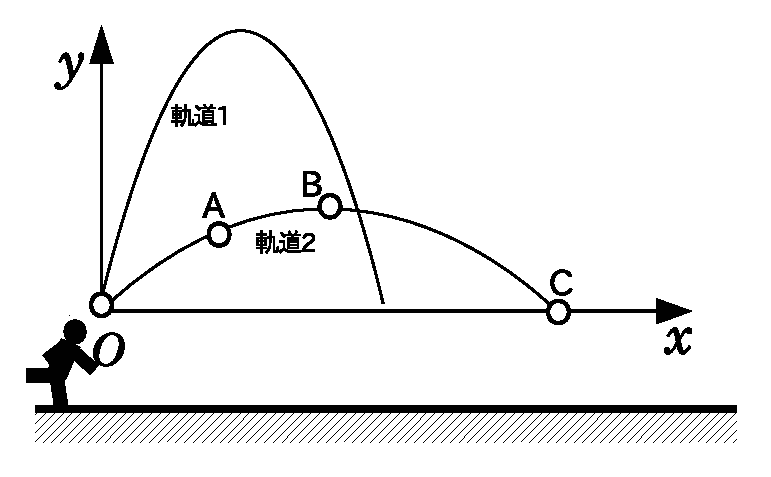
\includegraphics[width=7.0cm]{throwball.eps}
    \caption{ボールの斜め投げ上げ}\label{fig:throwball}
\end{figure}

軌道1のようにかなり上向きに投げ上げたら, 高くは上がるものの, 遠くには飛ばない。軌道2のように, 
若干水平ぎみに投げ上げたら, 高くは上がらないが, そこそこ遠くに飛ぶ。

\begin{q}\label{q:2Dthrow0} 軌道2で, A, B, Cのそれぞれの位置にボールが来た時を考える。
\begin{enumerate}
\item 速さが最も大きいのは, A, B, Cのうちどの位置のときか?
\item A, B, Cの各位置で, ボールにかかる合力を, 矢印で図に描き込め。
矢印の長さは適当でよいが, 複数の矢印どうしで長さはつじつまがあって
いなければならない(大きい力は長く, 小さい力は短く)。
\item A, B, Cの各位置で, ボールの加速度を, 点線矢印で図に描き込め。
矢印の長さは適当でよいが, 複数の矢印どうしで長さはつじつまがあって
いなければならない(大きい加速度は長く, 小さい加速度は短く)。
\item 加速度の大きさが最も大きいのは, A, B, Cのうちどの位置のときか?
\end{enumerate}
\end{q}

\begin{q}\label{q:2Dthrow}
どのような角度で投げ上げたら, 最も遠くまでボールを飛ばせるか, 考えよう。
君の位置を原点$O$とし, 水平方向に$x$軸, 鉛直方向に$y$軸をとる。 時刻を$t$とし, 君がボールを
手放した瞬間を$t=0$とする。$t=0$のときにボールの速度は$x$軸から角$\theta$の方向で, その大きさ
は$v_0$であったとする。

時刻$t$におけるボールの位置と速度をそれぞれ${\bf r}(t), {\bf v}(t)$とする。
重力加速度を$g$とする。
\begin{eqnarray*}{\bf r}(t)=(x(t), y(t))\end{eqnarray*}
とする。
\begin{enumerate}
\item ${\bf r}(0)=(0, 0)$, ${\bf v}(0)=(v_0\cos\theta, v_0\sin\theta)$であることを示せ。
\item ボールが手を離れてから地上に落ちるまでのボールの運動方程式は, 
次式のようになることを示せ:
\begin{eqnarray}
&&m\frac{d^2x}{dt^2}=0\label{eq:2Dthroweqmx}\\
&&m\frac{d^2y}{dt^2}=-mg\label{eq:2Dthroweqmy}
\end{eqnarray}
\item 上の微分方程式(\ref{eq:2Dthroweqmx}), (\ref{eq:2Dthroweqmy})を解くと, 
解はそれぞれ次式のようになることを示せ:
\begin{eqnarray}
&&x=(v_0\cos\theta)t\\
&&y=(v_0\sin\theta)t-\frac{1}{2}\,gt^2
\end{eqnarray}
\item 前問の結果から$t$を消去して次式を示せ:
\begin{eqnarray}
y=(\tan\theta)x-\frac{g}{2v_0^2\cos^2\theta}\,x^2\label{eq:throwtilt}
\end{eqnarray}
\item 前問の結果を, 横軸$x$, 縦軸$y$のグラフに描け。これがボールの軌跡だ。
\item 投げ上げたボールが着地する場所の$x$座標を$X$とすると, 次式を示せ:
\begin{eqnarray}
X=\frac{v_0^2\sin2\theta}{g}\label{eq:throwtiltX}
\end{eqnarray}
\item $v_0$が一定の時, 投げ上げの角$\theta$がどのくらいのとき, $X$は最大になるか? 
\end{enumerate}
\end{q}
\vspace{0.2cm}

\begin{q}\label{q:2Dthrow_hammer}
ハンマー投は, ハンマー(ワイヤーの先に質量7.26~kgの金属球がついたもの)を振り回して投げ上げ, 
飛ばした距離を競うスポーツである。世界記録は86.7~mである。投げ上げの角度が, 前問で求めた角に
一致していたと仮定して, 世界記録樹立時のハンマーの初速度を推定せよ。
\end{q}
\vspace{0.6cm}



\section{円運動}\index{えんうんどう@円運動}

一定の速さで円周上を一方向に動く運動のことを, 等速円運動という。

平面内の円運動を考えてみよう。$xy$座標系の中に質量$m$の質点があり, 何かの機構に
よって, 原点の方向に, 一定の大きさ$F$の力でひっぱられて
いるとしよう(図\ref{fig:circular_motion})。
\begin{figure}[h]
    \centering
    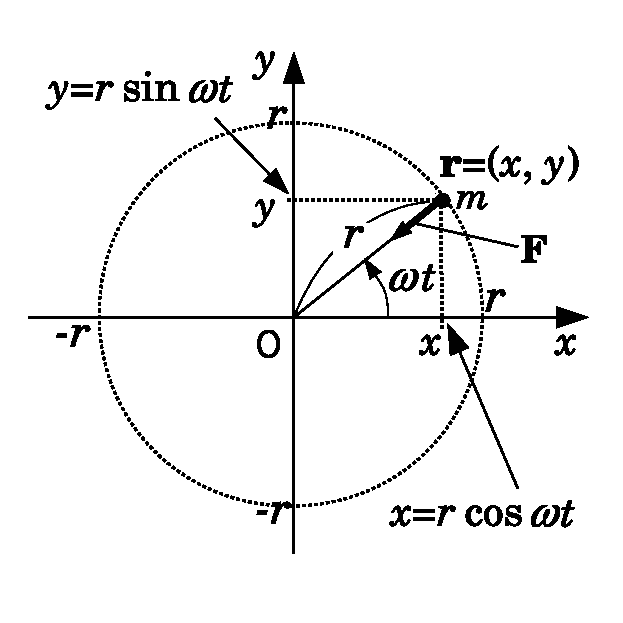
\includegraphics[width=7.0cm]{circular_motion.eps}
    \caption{等速円運動}\label{fig:circular_motion}
\end{figure}
うまく条件が揃えば, この質点は, 原点を中心とする半径$r$の円周上を
等速円運動する。そのことを証明しよう。

まず, 時刻$t$における質点の位置, 速度, 加速度をそれぞれ
\begin{eqnarray}
{\bf r}(t)&=&(x(t), y(t))\\
{\bf v}(t)&=&(v_x(t), v_y(t))\\
{\bf a}(t)&=&(a_x(t), a_y(t))
\end{eqnarray}
とし\footnote{前章でも述べたが, 位置ベクトルは, {\bf r}と書くことも多い。}, 
$t=0$で質点は$x$軸上の点$(r, 0)$にあるとする。すなわち, 
\begin{eqnarray}
{\bf r}(0)=(x(0), y(0))=(r, 0)
\end{eqnarray}
である。

\begin{q}\label{q:circle_motion}
\begin{enumerate}
\item 質点が実際にこの円周上を一定の角速度$\omega$で回転するならば
次式が成り立つことを示せ(ヒント: 極座標):
\begin{eqnarray}
&&{\bf r}(t)=(r\cos\omega t, r\sin\omega t)\label{eq:circle_motion_xy}\\
&&{\bf v}(t)=(-r\omega\sin\omega t, r\omega\cos\omega t)\label{eq:circle_motion_vxvy}\\
&&{\bf a}(t)=(-r\omega^2\cos\omega t, -r\omega^2\sin\omega t)\label{eq:circle_motion_axay}\,\,\,\,\,\,\,\\
&&{\bf a}(t)=-\omega^2{\bf r}(t)\label{eq:circle_motion_a}
\end{eqnarray}
\item 時刻$t$のとき質点に働く力${\bf F}(t)$は, 次式になることを示せ:
\begin{eqnarray}{\bf F}=(-F\cos\omega t, -F\sin\omega t)\end{eqnarray}
\item 質点の運動方程式は, 次式のようになることを示せ:
\begin{eqnarray}
-F\cos\omega t=ma_x(t)\label{eq:circle_motion_Fx}\\
-F\sin\omega t=ma_y(t)\label{eq:circle_motion_Fy}
\end{eqnarray}
\item \eref{eq:circle_motion_axay}で表される$a_x(t), a_y(t)$は, 
次式が成り立つときに限って上の運動方程式を満たす, ということを示せ。
\begin{eqnarray}
F=mr\omega^2\label{eq:mromegasq}
\end{eqnarray}
\item 質点の速度${\bf v}$の大きさ$v$は次式となることを示せ。
\begin{eqnarray}
v=r\omega\label{eq:circle_motion_v_romega}
\end{eqnarray}
\item \eref{eq:mromegasq}は, 次式のようにもできることを示せ:
\begin{eqnarray}
F=\frac{mv^2}{r}\label{eq:mvsqovr}
\end{eqnarray}
\item 質量と半径はそのままで, 速度の大きさ$v$が2倍になると, 力は何倍になるか? 
\item 質量と速度はそのままで, 半径$r$が1/2倍になると, 力は何倍になるか? 
\end{enumerate}
\end{q}
\vspace{0.2cm}

\begin{q}\label{q:car_slip}
前問の最後の結果から, 車を運転する時に, なぜカーブの手前で減速せねばならないか, 述べよ。
\end{q}
\vspace{0.2cm}

%向心力と遠心力



実は, 単振動と円運動は, 密接な関係がある。等速円運動の方程式の
ひとつである\eref{eq:circle_motion_a}を考えよう:
\begin{eqnarray*}
{\bf a}(t)=-\omega^2{\bf r}(t)
\end{eqnarray*}
この左辺は$d^2{\bf r}/dt^2$であり, さらに, ${\bf r}=(x, y)$とおけば, 上の式は, 
\begin{eqnarray}
&&\frac{d^2 x}{dt^2}=-\omega^2 x\\
&&\frac{d^2 y}{dt^2}=-\omega^2 y
\end{eqnarray}
となる。これらは, \eref{eq:vib}と同じ形, すなわち単振動の微分方程式
だ。従って, 等速円運動は, 2つの単振動 ($x$軸方向と$y$軸方向)
の組み合わせと考えることができる。実際, 等速円運動
\begin{eqnarray}\bigl(x(t), y(t)\bigr)=(r\cos\omega t, r\sin\omega t)\end{eqnarray}
について, その$x$座標だけを取り出した関数
\begin{eqnarray}x(t)=r\cos\omega t\end{eqnarray}
は, \eref{eq:spring_Acos}にそっくりだし, $y$座標だけを取り出した関数
\begin{eqnarray}y(t)=r\sin\omega t\end{eqnarray}
は, \eref{eq:spring_Asin}にそっくりだ。
従って, 角速度, 周期などの概念は, 円運動と単振動で共通だ。
ただし, 「角速度」の「角」は, 円運動の場合は幾何学的な意味が
直感的にわかりやすい。
\vspace{0.2cm}

\begin{q}\label{q:hammer_throw}
ハンマー投の世界記録樹立時(問\ref{q:2Dthrow_hammer}参照)に, 投擲者の腕にはどのくらいの力
がかかっただろうか? 
それは何kgの物体を持ち上げる力に相当するだろうか? 回転の半径を1.5~mと仮定せよ(有効数字2桁で十分)。
ヒント:\eref{eq:mvsqovr}。$m$や$v$の値は問\ref{q:2Dthrow_hammer}から流用する。
\end{q}
\vspace{0.2cm}

\begin{q}\label{q:sun_earth0}
太陽のまわりをまわる地球の円運動を考えよう。地球を質点とし, 地球の公転軌道を半径$r$
の円とし(厳密には楕円だが), その中心に太陽があるとし, 太陽は動かないと仮定する。
太陽と地球の質量をそれぞれ$M$, $m$とする。万有引力定数を$G$とする。
\begin{enumerate}
\item この円運動を維持するために地球が太陽から受ける力の大きさを, $r$, $\omega$, $m$であらわせ。
\item この力は万有引力によって実現される。このことから, 次式を示せ。ただし$\omega$は角速度である。
\begin{eqnarray}\omega=\sqrt{\frac{GM}{r^3}}\label{eq:circle_grav_omega}\end{eqnarray}
\item この円運動の周期$T$は, 次式のようになることを示せ:
\begin{eqnarray}T=2\pi\sqrt{\frac{r^3}{GM}}\label{eq:circle_grav_T}\end{eqnarray}
\item $r$, $G$, $M$に具体的な数値を代入して$\omega$の値を求め, 周期を求めよ。それは何日に相当するか? 
(計算に必要な数値は, 各自, 調べよ)
\end{enumerate}
\end{q}
\vspace{0.2cm}

\begin{q}\label{q:spaceship}
以下の宇宙飛行体は, それぞれ何時間で地球のまわりを一周するか? 地球の半径を6400 kmとし, 
地球や以下の飛行体を質点とみなす。()内は地表から飛行体への距離である。
\begin{enumerate}
\item 国際宇宙ステーション(約400 km)
\item 気象衛星ひまわり(約36000 km)
\end{enumerate}
\end{q}

気象衛星ひまわりは, 赤道上空の宇宙空間を, 地球の自転と同じ角速度で地球のまわりを
まわっているので, 常に地表の同じ場所の雲の様子を時々刻々と観測できる。
\mv

\begin{faq}{\small\textgt{自然界には, 円運動だけでなく楕円運動もあるのですか? もしあるなら, やはり運動方程式
で表せるのですか?} ... 
はい。惑星の公転は, 一般には円ではなく楕円であり, やはり運動方程式に従います。特に火星の楕円軌道は, 
「天体は真円運動をする」というオカルト的な中世の思い込みから脱皮してニュートン力学が生まれるための, 
重要な手がかりでした。また, GPS衛星を補完して測量精度を上げるための「みちびき」という日本の
人工衛星(その信号が農地のトラクターの自動運転などで使われている)は, 
気象衛星ひまわりの近くだけど楕円の軌道を動いています。}\end{faq}\mv

\begin{faq}{\small\textgt{公式がごちゃごちゃになってしまいます。。。} ... 
どの式がどの法則から派生するのか, という体系性を意識することが重要。物理学は
公式の羅列ではなく, 法則の体系ですから。}\end{faq}\mv

\begin{faq}{\small\textgt{高校の物理の先生が「物理ができるかどうかは
絵が上手に描けるかどうかで決まる」と言っていました。
確かに絵が上手に描けるとちょっとやる気もでます。。。} ... 
絵や文など, 自分を表現するツールを豊かに持っている人は, 
知的な成長が早いと思います。}\end{faq}\mv

\begin{faq}{\small\textgt{そもそも物の動きとか, わかって何が嬉しいのですか? 
そういうのって, 病気を治す薬とか, バイオ燃料を作る微生物とか, 乾燥に強い植物とかの
研究開発に関係あるのでしょうか?} ... そう短絡的に考えてはダメです。薬の働き方は
タンパク質の構造や, それが酸性度や温度でどう変わるか, などで決まります。それを
知るには, 結局は分子を構成する原子の「動き」が大事なのです。微生物の中の生体反応
も同じ。植物が水を吸い上げるときは, 結局は水分子が「どう動くか」が大事でしょ。
結局, 科学の本質は「動き」に代表される物理現象に帰着するのです。ここで学んでいる
のは, それらの基礎中の基礎です。}\end{faq}\mv

\begin{faq}{\small\textgt{そんなの屁理屈にしか聞こえませんが} ... 
屁理屈ではありませんよ。実際, 薬の分子の動態を, 膨大な数の方程式で表してコンピュータで
解析することが, 既に行われています。そうすることで, 試験管で実験するよりも効率的に, 
たくさんの分子を調べることができるのです。}\end{faq}\mv
\hv

\begin{exq} 
\begin{enumerate}
\item 自転車競技場(競輪場)のトラックのカーブ部分は斜面になっている。その理由を
物理学的に説明せよ。
\item 飛行機(旅客機)に乗ったことのある人は, 飛行機が旋回するとき, 機体を傾ける
ということを知っているだろう。飛行機が左に旋回するとき, 左の翼は上げるか, 下げるか?
その理由を物理学的に説明せよ。(1)とは違う理由であることに注意!
\item 無重力だが空気はある, という環境(国際宇宙ステーションの中など)で紙飛行機を飛ばしたら, どのような運動をするか?
\end{enumerate}
\end{exq}



\section{解答}
%
\noindent{\textbf{答}}\ref{q:harmonic_osci0}
$\omega=\sqrt{k/m}$より, 質量$m$が2倍になると, 角速度$\omega$は$1/\sqrt{2}\fallingdotseq0.71$倍になる
(つまり振動はゆっくりになる)。また, 周期を$T$とすると, $T=2\pi/\omega$だから, $T$は$\sqrt{2}\fallingdotseq1.4$倍になる。\mv

%
\noindent{\textbf{答}}\ref{q:harmonic_osci1}
\eref{eq:lincombvib3}で, $x(0)=X_0$, $x'(0)=0$とすると, $x(t)=X_0\cos\omega t$。
グラフは図\ref{fig:springX0}のようになる。
\begin{figure}[h]
    \centering
    \includegraphics[width=7cm]{springX0.eps}
    \caption{単振動する質点の位置の経時変化}\label{fig:springX0}
\end{figure}

%
\noindent{\textbf{答}}\ref{q:harmonic_osci2}
\eref{eq:lincombvib3}で, $x(0)=0$, $x'(0)=V_0$とすると, 
\begin{eqnarray}x(t)=\frac{V_0}{\omega}\sin\omega t\end{eqnarray}
となる。グラフは図\ref{fig:springV0}のようになる。\mv
\begin{figure}[h]
    \centering
    \includegraphics[width=7cm]{springV0.eps}
    \caption{単振動する質点の速度の経時変化}\label{fig:springV0}
\end{figure}

% 君は地表のある点から, 空にむかって, 斜め方向に質量
\noindent{\textbf{答}}\ref{q:2Dthrow0} 略。ヒント: 飛行中のボールに
働く力は重力のみ(空気抵抗は無視している)。\\

\noindent{\textbf{答}}\ref{q:2Dthrow}
${\bf r}(t)=(x(t), y(t))$, ${\bf v}(t)=(x'(t), y'(t))$となることに注意せよ。
\begin{enumerate}
\item ボールは時刻$t=0$で原点(君の位置)にあるから${\bf r}(0)=(0,0)$。
また, $|{\bf v}(0)|=v_0$で, ${\bf v}(0)$が$x$軸からなす角が$\theta$であること
から, 
\begin{eqnarray}{\bf v}(0)=(v_0\cos\theta, v_0\sin\theta)\end{eqnarray}
\item $x$方向には力が働かないので, \eref{eq:2Dthroweqmx}が成り立つ。
$y$方向には重力つまり$-mg$が働くので, \eref{eq:2Dthroweqmy}が成り立つ。
\item \eref{eq:2Dthroweqmx}を2回積分すると, 
\begin{eqnarray}x(t)=C_1t+C_2\end{eqnarray}
となる。ここで$C_1, C_2$は積分定数。
$x(0)=0$より$C_2=0$。$x'(0)=v_0\cos\theta$より, $C_1=v_0\cos\theta$。
従って, 
\begin{eqnarray}x(t)=(v_0\cos\theta)t\end{eqnarray}
\eref{eq:2Dthroweqmy}を2回積分すると, 
\begin{eqnarray}y(t)=-\frac{gt^2}{2}+C_3t+C_4\end{eqnarray}
となる。ここで$C_3, C_4$は積分定数。
$y(0)=0$より$C_4=0$。$y'(0)=v_0\sin\theta$より, $C_3=v_0\sin\theta$。
従って, 
\begin{eqnarray}y(t)=(v_0\sin\theta)t-\frac{gt^2}{2}\end{eqnarray}
\item 略(各自計算せよ)。
\item 図\ref{fig:throw_ball_slant}
\begin{figure}[h]
    \centering
    \includegraphics[width=8cm]{throw_ball_slant.eps}
    \caption{斜めに投げ上げられたボールの軌跡}\label{fig:throw_ball_slant}
\end{figure}
\item 略(\eref{eq:throwtilt}で$y=0$となるのは, $x=0$と\eref{eq:throwtiltX}
の場合であり, 前者は投げ上げの瞬間, 
後者は着地の瞬間に対応する。$2\cos\theta\sin\theta=\sin2\theta$に注意せよ。)
\item \eref{eq:throwtiltX}が最大になるのは, $\theta=\pi/4$, つまり45度のとき。
\end{enumerate}
\mv

\noindent{\textbf{答}}\ref{q:2Dthrow_hammer}
前問より, $\theta=\pi/4$が, ハンマー投擲の最適角度。このとき\eref{eq:throwtiltX}
は$X=v_0^2/g$となる。従って$v_0=\sqrt{gX}$。$X=86.7$~m, 
$g=9.8$~m~s$^{-2}$とすれば, $v_0=29.1$~m~s$^{-1}$。
\mv

% 平面内の円運動を考えてみよう
\noindent{\textbf{答}}\ref{q:circle_motion}
\begin{enumerate}
\item 略(数学リメディアル教材参照)
\item 原点から質点へのベクトル(つまり質点の位置ベクトル)は
\begin{eqnarray}
{\bf r}&=&(r\cos\omega t, r\sin\omega t)\nonumber\\
       &=&r(\cos\omega t, \sin\omega t)
\end{eqnarray}
だから, 原点から質点へ向かう単位ベクトルは$(\cos\omega t, \sin\omega t)$。問題の仮定より, 
質点にかかる力の方向は, 質点から原点への方向である。その方向の単位ベクトルは, 前述の単位ベクトル
の逆向きだから, $(-\cos\omega t, -\sin\omega t)$。力の大きさは$F$なので, 結局, 力を
あらわすベクトルは, 以下のようになる:
\begin{eqnarray}
{\bf F}(t)&=&F(-\cos\omega t, -\sin\omega t)\nonumber\\
          &=&(-F\cos\omega t, -F\sin\omega t)
\end{eqnarray}
\item 略($x, y$各方向の運動方程式を考えればよい)。
\item \eref{eq:circle_motion_axay}で表された$a_x(t), a_y(t)$を\eref{eq:circle_motion_Fx}, \eref{eq:circle_motion_Fy}に代入すれば, 
\begin{eqnarray}
-F\cos\omega t=-mr\omega^2\cos\omega t\\
-F\sin\omega t=-mr\omega^2\sin\omega t
\end{eqnarray}
となる。前者の両辺を$-\cos\omega t$で割ったり, 後者の両辺を$-\sin\omega t$で割ったり
すれば, $F=mr\omega^2$, すなわち\eref{eq:mromegasq}が成り立つ。逆に, \eref{eq:mromegasq}
が成り立てば, 上記の式が成り立つのは明らかだ。
\item 略(\eref{eq:circle_motion_vxvy}を使って$(v_x, v_y)$の大きさを求めるだけ)。
\item 略(\eref{eq:circle_motion_v_romega}と\eref{eq:mromegasq}から$\omega$を消去)。
\item \eref{eq:mvsqovr}より, 4倍。
\item \eref{eq:mvsqovr}より, 2倍。
\end{enumerate}
\mv

%
\noindent{\textbf{答}}\ref{q:car_slip}
タイヤは高速で転がっていても, 地面との接触面は常に地面と噛み合って
いるので, 接触面ではタイヤと地面は静止しているため, 摩擦力は静止摩擦力である。

さて, 車がカーブに入ると, その回転運動を維持するには, 前問の結果から, 
速度の二乗に比例した横向きの力を, 車のタイヤと地面の間での摩擦力で実現しなければ
ならない。従って, 高速度でカーブに入ると, 激しく大きな静止摩擦力が要求される。
それに耐えきれないと, タイヤと地面の間で滑りが起き, 突然, 摩擦力は静止摩擦力
から, より小さな動摩擦力に代わるので, 車はカーブを続けることができなくなる。
カーブに入ってから慌てて急ブレーキを踏むと, さらに大変なことになる。
ブレーキによってタイヤの回転が急に止まるので, 地面とタイヤの間での滑りが, 
より早い段階(車が減速する前)で起きてしまう。そのような事態になっては遅い。
それを避けるには, カーブへ進入する前に十分に減速する必要がある。万一, 
高速度でカーブに入ってしまったら, タイヤがスリップしないように気をつけて
ブレーキをじんわり踏みながら, 幸運を祈るしかない。
\mv

%
\noindent{\textbf{答}}\ref{q:hammer_throw}
投擲者がハンマーを手放す直前まで, ハンマーは回転運動している。その速度を
$v$とすると, \eref{eq:mvsqovr}より, $F=mv^2/r$の力が投擲者の腕にかかった
はずである。問\ref{q:2Dthrow_hammer}の問題文と結果より, $m=7.26$~kg, $v=29.1$~m~s$^{-1}$。$r=1.5$~mとすると, 
$F=4100$ N。これに相当する重力を受ける物体の質量は, この値を$g=9.8$~m~s$^{-2}$で
割って, 約420~kg。つまり約420~kgの物体を地上で持ち上げるのに必要な力に相当する。
\mv

%
\noindent{\textbf{答}}\ref{q:sun_earth0}
\begin{enumerate}
\item \eref{eq:mromegasq}より, $mr\omega^2$
\item 万有引力は$GMm/r^2$。従って, 
\begin{eqnarray}mr\omega^2=\frac{GMm}{r^2}\end{eqnarray}
これを$\omega$について解けば与式を得る。
\item $T=2\pi/\omega$より与式を得る。
\item $G=6.67408\times10^{-11}$ N~m$^2$~kg$^{-2}$, $M=1.9891\times10^{30}$~kg, 
$r=1.4960\times10^{11}$~mとすると, $\omega=1.99125\times10^{-7}$ Hz。
周期は, $2\pi/\omega=3.15539\times10^7$~s$=365.207$~日=$365.21$~日。
注: 実際の公転周期365.25~日と少しずれたのは, 地球は厳密には楕円軌道をしているため。
これを補正するには$r$の値に修正が必要。
注: 与えられた数値は有効数字5桁であっても, 途中計算は1桁余分にとって行い, 最後に5桁に丸める。
\end{enumerate}
\mv

%
\noindent{\textbf{答}}\ref{q:spaceship}
\eref{eq:circle_grav_T}において$M$を地球の質量とすればよい。
\begin{enumerate}
\item $r=6800$ kmとすると, $T=5580$ s$\fallingdotseq$1.6時間。
\item $r=42000$ kmとすると, $T=87000$ s$\fallingdotseq$24時間。
\end{enumerate}


%2011.4.3 ヤマサキ この章は大きく変更した箇所はありません。
\chapter{力学的エネルギー保存則(1)}\label{chapt:consenergy1}

運動の3法則, 特に運動方程式を使えば, 原理的には, どんな物体
のどんな運動も予測できる。しかし現実的には, 必要な計算量が膨大で手に
負えなかったり, 必要な情報が足りなかったりで, 運動方程式を解くのが
めんどくさかったり無理だったりすることが多い。そのような場合に便利なの
が, 本章で学ぶ「力学的エネルギー保存則」である。

この法則は, 運動方程式が姿を変えたものだが, 特定の状況下では, 
運動方程式を直接考えるよりも, ずっと簡単に運動の様子を教えてくれる(ことがある)。

もう少し詳しく説明しよう。本章では話を簡単にするために, 運動を
直線($x$軸上)に限定する。運動の第二法則, すなわち運動方程式によれば, 
質量$m$の質点が力$F$を受けて運動するとき, その運動は, 必ず以下のような運動方程式に従う:
\begin{eqnarray}F=ma\label{eq:F_ma_energy0}\end{eqnarray}
$a$は質点の加速度である(力と加速度はベクトルなので本来は${\bf F}$, ${\bf a}$
と太字で書くべきところだが, ここでは運動が1次元に限定されているので, 
$F$と$a$は細字で書いた)。加速度は速度を時刻で微分したものなので, この式は, 
以下のようにも書ける:
\begin{eqnarray}
F&=&m\frac{dv}{dt}\quad\quad\text{($t$は時刻, $v$は質点の速度)}\label{eq:F_ma_energy1}
\end{eqnarray}
\eref{eq:F_ma_energy0}と\eref{eq:F_ma_energy1}は, 加速度の表現が形式的に違うだけで, 
互いに等価な方程式であり, \eref{eq:motion}を直線運動(1次元の運動)に書き直したものだ。
以下, \eref{eq:F_ma_energy1}を議論の出発点としよう。\mv

いま, 直線($x$軸)上を, 力$F(t)$を受けて, 質量$m$の質点が, 時刻$t_0$から$t_1$の
間で何らかの運動をしている状況を考えよう。この運動は, もちろん\eref{eq:F_ma_energy1}に
従うので, \eref{eq:F_ma_energy1}を解いて, 位置と速度を時々刻々と追跡すれば, 
運動の全体像が判明する。でも, 微分方程式を解くのは, たいてい, めんどくさい。

もっと楽ができないだろうか? たとえば, 物騒な話だが, 
砲弾やミサイルをどこかに命中させたい場合は, 「時々刻々」でなくてよいから, 
最初と最後だけでの位置(と, できれば速度...衝撃の大きさを
知りたいから!)がわかれば十分である。

そこで, 運動方程式の経過の詳細に立ち入ることなしに, 運動の最初($t=t_0$)と
最後($t=t_1$)の間に何らかの関係を見いだせないだろうか? 実は, 
\eref{eq:F_ma_energy1}をうまく数学的に変形すれば, そのような関係を見出す
ことができるのだ。


これを理解するのには, 先に学んだ「ポテンシャルエネルギー」という概念と, 
今から学ぶ「運動エネルギー」という概念である。\\


\section{運動エネルギー}\label{sect:1D_kinetic_energy}\index{うんどうえねるぎー@運動エネルギー}

\begin{itembox}{1次元運動における運動エネルギーの定義}
質量$m$の質点が速度$v$で運動するとき, 次式をその質点の運動エネルギー(kinetic energy)という。
\begin{eqnarray} 
\frac{1}{2}\,mv^2\label{eq:kineticEnergy0}
\end{eqnarray}
\end{itembox}

\begin{q}\label{q:kinetic_energy}
\eref{eq:kineticEnergy0}を5回書いて記憶せよ。\end{q}

上の式は速度$v$の関数である(質量$m$の関数でもあるが, 
多くの場合, 質点の質量は不変なので, ここでは$m$は定数としておこう)。
そこで, 慣習的には運動エネルギーを関数$T(v)$と表すことが多い:
\begin{eqnarray} 
T(v)=\frac{1}{2}\,mv^2\label{eq:kineticEnergy}
\end{eqnarray}

この「運動エネルギー」なるものがどのように活躍するかをこれから説明する。
まず, 質点の位置を$x$とする。速度$v$は位置$x$を時刻$t$で微分したもの
(それが速度の定義!)だから, 
\begin{eqnarray}
\frac{dx}{dt}=v\label{eq:energy_def_velocity}
\end{eqnarray}
である。両辺に$dt$をかけると, 
\begin{eqnarray}
dx= v\,dt\label{eq:dv_vdt}
\end{eqnarray}
となる。つまり, $x$の微小変化$dx$は, 速度$v$に時間の微小変化$dt$をかけたものである。

さて, \eref{eq:F_ma_energy1}の両辺に$dx$をかけてみよう:
\begin{eqnarray} 
F\,dx= m\frac{dv}{dt}\,dx\label{eq:WandT00}
\end{eqnarray} 
この右辺の$dx$を, \eref{eq:dv_vdt}で書き換えれば, 次式を得る:
\begin{eqnarray} 
F\,dx= m\frac{dv}{dt}v\,dt\label{eq:WandT000}
\end{eqnarray} 

ここで, 時刻$t_0$から$t_1$までの運動を, たくさんの短い断片に分割し, 
それぞれの断片で\eref{eq:WandT000}を考えて足し合わせる。つまり, 
時刻$t_0$から$t_1$までの間で, \eref{eq:WandT000}を積分すると, 
\begin{eqnarray} 
\int_{x_0}^{x_1}F\,dx=\int_{t_0}^{t_1}m\frac{dv}{dt}\,v\,dt\label{eq:WandT00s}
\end{eqnarray} 
となる。$x_0=x(t_0), x_1=x(t_1)$とした。ここで置換積分によって右辺の積分変数を$t$から$v$に変換すると\footnote{形式的には
右辺の$dt$を約分することに相当する。}, 
\begin{eqnarray} 
\int_{x_0}^{x_1}F\,dx=\int_{v_0}^{v_1}mv\,dv
\end{eqnarray} 
となる。$v_0=v(t_0), v_1=v(t_1)$とした。
この左辺は, 質点が$x_0$から$x_1$に移動する際に力がなす仕事$W_{01}$である(わからない人は\eref{eq:work2}を見よ)。
一方, 右辺は, 
\begin{eqnarray}=\left[\frac{1}{2}\,mv^2\right]_{v_0}^{v_1}=\frac{1}{2}\,mv_1^2-\frac{1}{2}\,mv_0^2\end{eqnarray}
となる。以上より, 
\begin{eqnarray} 
W_{01}=\frac{1}{2}\,mv_1^2-\frac{1}{2}\,mv_0^2\label{eq:WandT0}
\end{eqnarray} 
である。右辺に運動エネルギーが出てきたではないか!

式(\ref{eq:WandT0})を, \eref{eq:kineticEnergy}を使って書き換えると, 
\begin{eqnarray} 
W_{01}=T(v_1)-T(v_0)\label{eq:WandT2}
\end{eqnarray} 
あるいは, 同じことだが, 
\begin{eqnarray} 
T(v_1)=T(v_0)+W_{01}\label{eq:TandW2}
\end{eqnarray} 
となる。この式は味わい深い。質点にかかる力がなした仕事は, 質点の運動エネルギーの変化
に等しい。つまり, 仕事がされるぶんだけ, 運動エネルギーが増えるのだ。そう考えると, 
運動エネルギーは仕事と等価な物理量, つまり「エネルギー」の名にふさわしい。
運動エネルギーは, 「質量を持つ物体の運動」という姿をまとったエネルギーである。\mv

ここで, 運動エネルギーの定義\eref{eq:kineticEnergy0}を再度よく見よう。
速度$v$が\underline{2乗}の形で入っている。従って, 運動エネルギーは, 速度$v$の符号(つまり方向)によらず, 速度$v$の
大きさ, つまり「速さ」だけで決まる。つまり, 運動エネルギーは、大きさは持つが
向きは持たない量, つまりスカラーである。質点がどのような方向に進んでいようが, 
運動エネルギーは速さ(と質点の質量)だけで決まるのだ。\mv
%

\begin{q}\label{q:principle_energy} \eref{eq:WandT0}を導出せよ。ヒント: 
\eref{eq:energy_def_velocity}以下の議論を整理して再現すればよい。\end{q}


さて, \eref{eq:WandT0}は, 運動方程式を位置(変位)で積分したものにすぎない
(高校物理では\eref{eq:WandT0}を「エネルギーの原理」と呼ぶらしいが, 大学では
そのような呼び方はほとんどしない)。
しかし, その有用性はハンパではない。\eref{eq:WandT0}を使えば, 
運動の過程を気にすることなく, 運動の最初の状態から最後の状態を直接的に
導くことができるのだ。以下の例でそれを学ぼう。\mv


%
\begin{q}\label{q:accel_energy}
質量$m$の質点が, 一定の力$F$を受けて, 一定の加速度$a$で直線($x$軸)上を運動している。時刻$t$
における位置と速度をそれぞれ$x(t), v(t)$とする。
\begin{enumerate}
\item 時刻$t_0$から時刻$t_1$の間に, 力$F$がなした仕事$W_{01}$は次式の
ようになることを示せ:
\begin{eqnarray}
W_{01}=F\{x(t_1)-x(t_0)\}
\end{eqnarray}
\item 次式を示せ:
\begin{eqnarray}
W_{01}=ma\{x(t_1)-x(t_0)\}
\end{eqnarray}
\item 以上と\eref{eq:WandT0}より, 次式を示せ
\footnote{これは高校物理で「$v^2-v_0^2=2ax$」と言われる公式だ。高校では
暗記させられる式だが, 実はこのように簡単に導出できる公式なので, 諸君は
もちろん暗記する必要は無い。本当に重要で記憶すべきなのは運動の三法則だ。
もしも, \eref{eq:v2_dist}を覚えていながら運動の三法則を言えないという人
がいたとしたら, その人は, 物理学の学びかたをなんか間違えている。}:
\begin{eqnarray}
v(t_1)^2-v(t_0)^2=2a\{x(t_1)-x(t_0)\}\label{eq:v2_dist}
\end{eqnarray}
\end{enumerate}
\end{q}
\vspace{0.4cm}

%
\begin{q}\label{q:curling2}
カーリングの問題(問\ref{q:curling})をもう一度考えてみよう。\index{かーりんぐ@カーリング}
初速度$v_0$で放されたストーンが距離$x$だけ進んで停止したとすると, 
\begin{enumerate}
\item ストーンが放されてから止まるまでの間に摩擦力がした仕事は$-F_{\text m}x$であることを示せ。
\item ストーンが放されてから止まるまでの間の運動エネルギーの変化は
\begin{eqnarray}0-\frac{1}{2}\,mv_0^2\end{eqnarray}
であることを示せ。ヒント:止まったとき速度は0。
\item 以上より, 次式を導け:
\begin{eqnarray}F_{\text m}=\frac{mv_0^2}{2x}\end{eqnarray}
これは\eref{eq:stoneFm}に一致する。
\item ストーンの到達距離が, 初速度の2乗に比例することを示せ。
\end{enumerate}
\end{q}
\vspace{0.4cm}

%
\begin{q}\label{q:meteorite}
地球のはるか遠方に静止している質量$m$の隕石が, 地球の重力に引かれて徐々に加速しながら
一直線に地球に向かってきたとする。我々は, 隕石を迎撃する計画を立てねばならない。そのためには, 
隕石が地球に衝突する直前の速さ$v_1$を求めねばならない。地球の質量を$M$, 半径を$R$とし, 
万有引力定数を$G$とし, 隕石を質点とみなす。
\begin{enumerate}
\item 隕石が, 無限遠方から, 地球の表面(中心から距離$R$)まで, 地球の重力に引かれてやってくるとき, 
地球の重力がなす仕事$W$は, 
\begin{eqnarray}
W=\frac{GMm}{R}\label{eq:meteorite1}
\end{eqnarray}
となることを示せ。
\item 隕石が無限遠方から地球表面までやってくるとき, 隕石の運動エネルギーの変化は次式であることを示せ。
\begin{eqnarray}
\frac{mv_1^2}{2}\label{eq:meteorite2}
\end{eqnarray}
ヒント:初速度は0である。
\item このことから, 地球衝突直前の隕石の速さ$v_1$は次式のようになることを示せ:
\begin{eqnarray}v_1=\sqrt{\frac{2GM}{R}}\end{eqnarray}
\item 上の式の定数に, 適切な数値を代入し, $v_1$の値を求めよ。
\end{enumerate}
\end{q}
\hv



\section{力学的エネルギー保存則}\index{りきがくてきえねるぎーほぞんそく@力学的エネルギー保存則}

前節の\eref{eq:WandT2}, \eref{eq:TandW2}で, 
「運動エネルギー$T$は, される仕事のぶんだけ増える」ことを学んだ。
さて, ここで以前学んだ, ポテンシャルエネルギーを思い出そう: ある特定の位置(基準点)
から位置$x$まで質点を運ぶときに保存力がなす仕事を$W(x)$とすると, ポテンシャルエネルギー
$U(x)$は, $U(x)=-W(x)$と定義された。ここで, $W(x_1)$は, 基準点から
まず$x_0$まで運んだときの仕事$W(x_0)$と, そこからさらに$x_1$まで運ぶときの仕事$W_{01}$
の総和である, と考えれば, 
\begin{eqnarray} 
W(x_0)+W_{01}=W(x_1)
\end{eqnarray} 
である。従って, 
\begin{eqnarray} 
W_{01}=W(x_1)-W(x_0)
\end{eqnarray} 
である。ところが, ポテンシャルエネルギーの定義から, 
\begin{eqnarray} 
W(x_0)=-U(x_0),\,\,\,\, W(x_1)=-U(x_1)
\end{eqnarray} 
とできるので, 結局, 
\begin{eqnarray} 
W_{01}=-U(x_1)+U(x_0)\label{eq:W01U1U0}
\end{eqnarray} 
である。これを\eref{eq:WandT0}に代入すれば, 
\begin{eqnarray} 
-U(x_1)+U(x_0)=\frac{1}{2}\,mv_1^2-\frac{1}{2}\,mv_0^2
\end{eqnarray} 
となる。これを整理すると, 
\begin{eqnarray} 
\frac{1}{2}\,mv_0^2+U(x_0)=\frac{1}{2}\,mv_1^2+U(x_1)\label{eq:DEcons}
\end{eqnarray} 
となる。あるいは, 運動エネルギー$T(v)$を使って書き換えれば, 
\begin{eqnarray} 
T(v_0)+U(x_0)=T(v_1)+U(x_1)\label{eq:DEcons2}
\end{eqnarray} 
となる。これらの式は味わい深い。左辺は質点が$x_0$にあるときの, 運動エネルギーとポテンシャルエネルギーの
和であり, 右辺は質点が$x_1$にあるときの, 運動エネルギーとポテンシャルエネルギーの和である。これらが
等しいということは, つまり, 「運動エネルギーとポテンシャルエネルギーの和」
(これを\underline{力学的エネルギー}\index{りきがくてきえねるぎー@力学的エネルギー}という)
は運動の始めから終わりまで一定である, ということである($x_0$や$x_1$は運動の最中のどこの位置を選んでも
よいことに注意せよ)。これを「力学的エネルギー保存則」と呼ぶ。ただし, 既に述べたように, 
仕事とポテンシャルエネルギーの変化がきちんと対応するのは, 働く力が「保存力」のときだけだ。
摩擦力のような非保存力が働く場合は, 仕事とポテンシャルエネルギーの変化が対応しないために, 
力学的エネルギー保存則が成り立つ保証は無い。まとめると, 
\begin{itembox}{力学的エネルギー保存則}
保存力だけが働く場合(非保存力が働かない場合), 
力学的エネルギー(運動エネルギーとポテンシャルエネルギーの和)
は運動の初めから終わりまで常に一定である。
\end{itembox}

%
\begin{q}\label{q:dynamic_energy}  
\begin{enumerate}
\item 力学的エネルギーとは何か? 
\item 力学的エネルギー保存則とは何か?
\item 力学的エネルギー保存則が成り立たないのはどういう場合か?
\end{enumerate}
\end{q}
\vspace{0.2cm}

%
\begin{q}\label{q:dynamic_energy_freefall}
鉛直線上を自由落下する質点の運動(空気抵抗無し)を例にとって, 力学的エネルギー保存則が成り立つ
ことを確かめよう。問\ref{q:freefall1}の状況を考える。$t=0$で$v=0$, $x=0$とすると, 
\begin{eqnarray} 
v(t)&=&-gt\label{eq:dynamic_energy_freefall1}\\
x(t)&=&-\frac{1}{2}\,gt^2\label{eq:dynamic_energy_freefall2}
\end{eqnarray} 
である。
\begin{enumerate}
\item 時刻$t$のときの質点の運動エネルギー$T$と(重力による)ポテンシャルエネルギー$U$はそれぞれ, 
\begin{eqnarray} 
T&=&\frac{1}{2}\,mg^2t^2\label{eq:dynamic_energy_freefallT}\\
U&=&-\frac{1}{2}\,mg^2t^2\label{eq:dynamic_energy_freefallU}
\end{eqnarray} 
となることを示せ。
\item 力学的エネルギー保存則を知らなかったことにして, 次式が恒等的に成り立つことを示せ:
\begin{eqnarray} 
T+U=0
\end{eqnarray} 
\end{enumerate}
\end{q}
\vspace{0.2cm}

%
\begin{q}\label{q:spring_vibration_energy}
バネにつけられて振動する質点の運動(単振動)を例にとって, 力学的エネルギー保存則が成り立つ
ことを確かめよう。前章の図\ref{fig:spring_vib}の状況を考える。時刻$t$での質点の位置と
速度をそれぞれ$x(t)$, $v(t)$とする。$t=0$で$v=0$, $x=x_0$とすると, 
\begin{eqnarray} 
x(t)=x_0\cos\omega t\label{eq:spring_vibration_energyx}
\end{eqnarray} 
である。ここで$\omega=\sqrt{k/m}$である。
\begin{enumerate}
\item 時刻$t$のときの質点の速度$v(t)$は次式になることを示せ(ヒント:$x(t)$を$t$で微分):
\begin{eqnarray} 
v(t)=-x_0\omega\sin\omega t\label{eq:spring_vibration_energyv}
\end{eqnarray} 
\item 時刻$t$のときの質点の運動エネルギー$T$と(バネの力による)ポテンシャルエネルギー$U$はそれぞれ, 
\begin{eqnarray}
T&=&\frac{1}{2}\,mx_0^2\omega^2\sin^2\omega t\label{eq:spring_vibration_energyT}\\
U&=&\frac{1}{2}\,kx_0^2\cos^2\omega t\label{eq:spring_vibration_energyU}
\end{eqnarray}
となることを示せ。ただしポテンシャルエネルギーの基準点として, ばねが自然状態
のときの質点の位置(つまり$x=0$)を考える。ヒント:$U=kx^2/2$の$x$に$x(t)$の式を代入。
\item 力学的エネルギー保存則を知らなかったことにして, 次式が恒等的に成り立つことを示せ:
\begin{eqnarray} 
T+U=\frac{1}{2}\,kx_0^2
\end{eqnarray} 
\end{enumerate}
\end{q}

問\ref{q:dynamic_energy_freefall}, 問\ref{q:spring_vibration_energy}では, 
力学的エネルギー保存則が成り立った。そうなったのは, これらの問で
働く力が保存力だけだったからだ。しかし, 以下のように, 非保存力が働くような
場合は力学的エネルギー保存則は成り立たない(というか適用されない):
\vspace{0.2cm}

\begin{q}\label{q:curling3} カーリングの問題, すなわち問\ref{q:curling}, 問\ref{q:curling2}で, 
力学的エネルギー保存則が成り立たないことを示せ。成り立たないのはなぜなのだろうか?
\end{q}
\vspace{0.2cm}

%
\begin{q}\label{q:bungy}
夏休みに南の島に行った君は, なぜか筑波大生の勇気を証明するために, バンジージャンプ
\index{ばんじーじゃんぷ@バンジージャンプ}をする
羽目になった。深い渓谷の上にかけられた橋から, ゴムバンドが垂れ下がっている。橋から渓谷の底までの高さは
50~m, ゴムバンドの長さ$L$は20~mくらいある。ゴムバンドは十分に軽い。ゴムバンドの先端が, 質量
60~kgの君の体につけられたとき, 君の脳裏に, 「こんなにゴムバンドが長ければ, 自分の体は途中
で止まらずに渓谷の底に叩きつけられるのではないか? 」という不安がよぎった。
\begin{figure}[h]
    \centering
    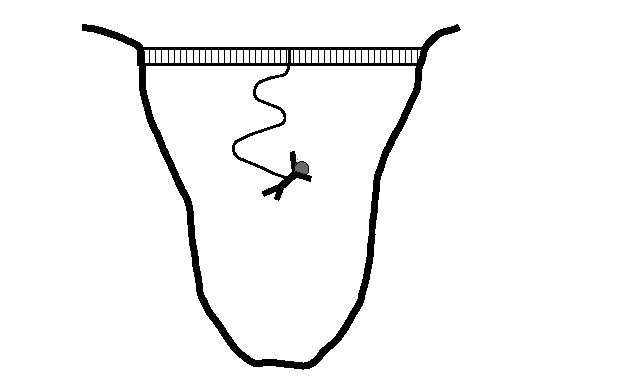
\includegraphics[width=6.0cm]{bangy.eps}
    \caption{問\ref{q:bungy}のバンジージャンプ。}\label{fig:bangy}
\end{figure}

そこで本番前に, 試しに, このゴムバンドを1.0~mだけ橋から出して, 静かに自分の体を吊り下げてみたら, 0.20~mだけ伸びた。
\begin{enumerate}
\item この1.0~mのゴムバンドのバネ定数$k_0$は?
\item 20~mのゴムバンドは均一の素材・太さであるとすると, 20~mのゴムバンドのバネ定数$k$は?
\suspend{enumerate}
 橋から初速度0で飛び降りるとき, 君の運動エネルギー$T$は0だ。重力のポテンシャルエネルギー$U$も0であるとする(つまり, 
飛び降りる地点を基準点とする)。
このとき, 当然ながら力学的エネルギー$E_0$は0だ。また, 橋から高さ$x$だけ落ちたとき, 
重力のポテンシャルエネルギーは$-mgx$である。そのときの速度を$v$とする。
\resume{enumerate}
\item 落下距離$x$がゴムバンドの長さ未満のとき, 力学的エネルギー$E_1$は, 
\begin{eqnarray} 
E_1=\frac{mv^2}{2}-mgx
\end{eqnarray} 
であることを示せ。このとき, ゴムバンドには全く力がかかっていないことに注意せよ。
\item 落下距離$x$がゴムバンドの長さを越えたら, 力学的エネルギー$E_2$は, 
\begin{eqnarray} 
E_2=\frac{mv^2}{2}-mgx+\frac{k(x-L)^2}{2}
\end{eqnarray} 
であることを示せ。
\item 君の体が運よく谷底の手前で停止したとするなら, 停止の瞬間の力学的エネルギー$E_3$は
\begin{eqnarray} 
E_3=-mgx+\frac{k(x-L)^2}{2}
\end{eqnarray} 
であることを示せ。
\item 以上を利用し, 力学的エネルギー保存の法則($E_0=E_3$)から, 停止点までの落下距離$x$を求めよ。
この結果から, 君はこのバンジージャンプを安全と判断するか? (注:実際に実験したいと思った人へ:やめとけ。)
\end{enumerate}
\end{q}
\vspace{0.4cm}


\section{物理学における保存則}\index{ほぞんそく@保存則}

力学的エネルギー保存則は保存力だけが関与するような運動に限って成立するが, 実は, 
「エネルギー保存則」は, もっと一般的・普遍的な法則である。たとえば, 
氷上を滑るカーリングのストーンは, 氷とストーンの間の摩擦力(非保存力)の仕事によって, 
いずれ停止してしまうが, このとき力学的エネルギーは一定ではない。ストーンの運動エネルギーは
ポテンシャルエネルギーに転換されないのだ。しかし, そのかわりに, ストーンの運動エネルギー
は氷とストーンの界面の摩擦によって熱に変わる。熱はエネルギーのひとつの形態だ。
そして熱エネルギーとストーンの運動エネルギーの合計は, 運動の最初・途中・最後のどの時点
でも一定である。つまり, 力学的エネルギーだけでは一定でないが, 「力学的エネルギー+熱エネルギー」
は一定なのだ。

熱エネルギー以外にも, 化学エネルギーや電気的・磁気的なエネルギーなど, 様々なエネルギーの
形態がある。実は質量もエネルギーの形態のひとつだ。ここでは詳述しないが, 
\begin{eqnarray}E=mc^2\end{eqnarray}
という式が, 質量とエネルギーの関係を表す($E$はエネルギー, $m$は質量, $c$は光の速さ)。
それらをすべて勘案すれば, エネルギーは決して無くなることはない。これをエネルギー保存則という。
エネルギー保存則は, ニュートン力学だけでなく, 様々な物理法則に対して成り立つ, 普遍的な
法則である。

物理学では, エネルギーのように, 様々な複雑な運動や反応の過程で最初から最後まで一定で
あるような量をとても大切にする。万物流転, 栄枯盛衰の世にあって, 変わらない何かを
求めようとするのは人間の普遍的な心理なのかもしれないが, 実際, 自然現象の中には, 
そのような「総和は変わらない(どこかで減った分はどこかで増えるような)特別な量」
(不変量)というものが, いくつか存在する。そのような事実(法則)を「保存則」と
呼ぶ。エネルギー保存則はその例だが, それ以外にも, 以下のような例がある(理由や
背景は今は理解しなくてもよい。そのようなものがある, ということを頭の片隅に留めて
おこう):
\begin{itemize}
\item 質量保存則
\item 電荷保存則
\item 運動量保存則
\item 角運動量保存則
\end{itemize}
ただし, 非保存力が働くときに力学的エネルギー保存則が破れるのと同様に, 
これら保存則の中には, 条件次第で「破れる」ものもある\footnote{例えば質量保存則は, 
核分裂や核融合等の反応では成り立たない。その過程では質量がエネルギーに変わってしまう
のだ。ただし, 質量保存則をエネルギー保存則と組み合わせてしまえば, その場合でも保存則
は成り立つ。}。

なぜ物理学では保存則を大切にするのか? それは, 君が勉強を進めて, 保存則の
持つ威力を知るに従って, おのずと明らかになるだろう。\mv

\begin{q}\label{q:drive_speed} 自動車の運転免許講習では, 
ことあるごとに「スピードを控えめに」と言われるが, なぜだろう? 
ひとつは, 高速での運動は制御が難しい, ということだ。運転者が
危険を察知してからブレーキを踏んだりハンドルを切ったりするまでには
時間がかかり, その間にも車は進んでしまう, というやつだ。しかし
それだけではない。スピードを控えめにすべき理由を, エネルギー保存則
の観点で説明せよ。\end{q}
\hv

\begin{exq} バネじかけのおもちゃの鉄砲を作った。銃身の中に仕込まれたバネのバネ定数は40~N/mである。
バネを10~cmだけ縮めて, 4.0~gの砲弾を仕込み, 引き金を引いた。砲弾はどのくらいの速さで
鉄砲から飛び出るか? ただし砲身は水平に固定され, バネの質量や, 砲身と砲弾の間の摩擦は
無視する。ヒント: バネのポテンシャルエネルギーの式は, 導出せずに使ってよい。\end{exq}

\begin{exq} 1辺の長さが100~mのピラミッドを作るのに必要最低限のエネルギーを
求めよ。ただしピラミッドは密度2.5~g~cm$^{-3}$の石が隙間なく積み上げられた
ものとし, 建築前にそれらの石はピラミッド底面と同じ高さにあったものと
する。ピラミッドの形は正八面体の上半分であるとする。ヒント: 積分が必要。\end{exq}

\begin{exq} 直径4.0~mm, 長さ10~cmの鉄製の釘を, 木材に打ち込む。質量$1.0$~kgのハンマーを, 
釘の頭から30~cmだけ高い位置から振り下ろして釘を叩くことを10回行ったら, 釘の頭は木の表面まで
届いた。このとき, 釘の頭を触ると熱かった。釘の温度は, 当初よりどれだけ上がったか? ただし, 
ハンマーを振り下ろすとき手は力を加えない(ハンマーの自由落下に任せる)。また, 木の熱伝導率
は鉄のそれよりもはるかに小さいので, 生じた熱の全ては釘に蓄えられ, 木には行かないとする。
鉄の密度を$\rho=7.8$~g~cm$^{-3}$, 鉄の比熱を460~J~kg$^{-1}$~K$^{-1}$とする。\end{exq}

\section{解答}
% 運動エネルギーとは何か? 
\noindent{\textbf{答}}\ref{q:kinetic_energy}
\eref{eq:kineticEnergy}で定義される$T$のこと(レポートではその式をきちんと書くこと!)。
\vspace{0.4cm}

% 質量$m$の質点が, 一定の力$F$を受けて, 一定の加速度$a$で運
\noindent{\textbf{答}}\ref{q:accel_energy}
\begin{enumerate}
\item 質点が受ける力は一定値$F$なので, 
\begin{eqnarray*}W_{01}=\int_{x(t_0)}^{x(t_1)}Fdx=\Bigl[Fx\Bigr]_{x(t_0)}^{x(t_1)}=F\{x(t_1)-x(t_0)\}\end{eqnarray*}
\item $F=ma$を上の式に代入すればよい。
\item \eref{eq:WandT0}を用いて$W_{01}$を消去する:
\begin{eqnarray*}
\frac{1}{2}mv(t_1)^2-\frac{1}{2}mv(t_0)^2=ma\{x(t_1)-x(t_0)\}
\end{eqnarray*}
両辺を2倍して$m$で割れば, 与式を得る。
\end{enumerate}
\vspace{0.4cm}

% 問\ref{q:curling}(カーリングの問題)をもう一度考えてみよう。
\noindent{\textbf{答}}\ref{q:curling2}
注意:手放されて滑っているストーンにかかる力は, 重力と, 氷面から受ける垂直抗力, 
そして動摩擦力だ。このうち, 重力と, 氷面から受ける垂直抗力は互いに逆向きで同じ
大きさであり, 打ち消しあう。従って, ストーンの運動には, 動摩擦力だけを考えれば良い。
\begin{enumerate}
\item 摩擦力(動摩擦力)はストーンの動く向きと逆方向で, $-F_{\text m}$。これを$F$として
問\ref{q:accel_energy}(1)の結果に入れれば, 仕事は$-F_{\text m}x$。
\item ストーンが放たれた直後の運動エネルギーは$mv_0^2/2$であり, 停止時には0。
従って与式が成り立つ。
\item \eref{eq:WandT0}によれば, 小問(1)の式と小問(2)の式は互いに等しい。従って与式を得る。
\item 小問(3)の結果から, 
\begin{eqnarray}x=\frac{mv_0^2}{2F_{\text m}}\end{eqnarray}
従って, $x$は$v_0^2$に比例する。
\end{enumerate}
\vspace{0.4cm}

% 地球のはるか遠方に静止している質量$m$の隕石が, 地球の
\noindent{\textbf{答}}\ref{q:meteorite}
\begin{enumerate}
\item \eref{eq:work_gravity}で, $R_0=\infty$, $R_1=R$とすればよい。
\item 略。
\item \eref{eq:WandT2}より, \eref{eq:meteorite1}と\eref{eq:meteorite2}が等しい。従って, 
\begin{eqnarray}\frac{GMm}{R}=\frac{1}{2}mv_1^2\end{eqnarray}
従って, 
\begin{eqnarray}v_1=\sqrt{\frac{2GM}{R}}\end{eqnarray}
\item $G=6.67\times10^{-11}$ N~m$^2$~kg$^{-2}$, \\
$M=5.97\times10^{24}$~kg, \\
$R=6.38\times10^{6}$~mとすると, \\
$v_1=1.12\times10^4$~m~s$^{-1}$。これは約40000 km/h。注:これを第二宇宙速度という。
\end{enumerate}
\vspace{0.4cm}

%
\noindent{\textbf{答}}\ref{q:dynamic_energy}
\begin{enumerate}
\item 運動エネルギーとポテンシャルエネルギーの和を力学的エネルギーという。
\item 力学的エネルギーは運動の初めから終わりまで一定である, という法則。
ただし, 力は保存力に限る。
\item 例えば摩擦力は保存力ではないから, 摩擦力が関与する運動では
力学的エネルギー保存則は成り立たない。
\end{enumerate}

% 鉛直線上を自由落下する質点の運動(空気抵抗
\noindent{\textbf{答}}\ref{q:dynamic_energy_freefall}
\begin{enumerate}
\item \eref{eq:kineticEnergy}に\eref{eq:dynamic_energy_freefall1}を代入すると, 
\eref{eq:dynamic_energy_freefallT}を得る。また, \eref{eq:potential_g}で, $h$を$x$と書き換えると, $U(x)=mgx$である。
この式に\eref{eq:dynamic_energy_freefall2}を代入すると, 
\eref{eq:dynamic_energy_freefallU}を得る。
\item \eref{eq:dynamic_energy_freefallT}と\eref{eq:dynamic_energy_freefallU}の辺々を
加えると与式を得る。
\end{enumerate}

% バネにつけられて振動する質点の運動(
\noindent{\textbf{答}}\ref{q:spring_vibration_energy}
\begin{enumerate}
\item 略(\eref{eq:spring_vibration_energyx}を$t$で微分するだけ)。
\item \eref{eq:kineticEnergy}に\eref{eq:spring_vibration_energyv}を代入すると, 
\eref{eq:spring_vibration_energyT}を得る。また, \eref{eq:potential_spring}に
\eref{eq:spring_vibration_energyx}を代入すると, 
\eref{eq:spring_vibration_energyU}を得る。
\item 
\eref{eq:spring_vibration_energyT}と
\eref{eq:spring_vibration_energyU}の辺々を加えると,
\begin{eqnarray*}
T+U=\frac{1}{2}mx_0^2\omega^2\sin^2\omega t+\frac{1}{2}kx_0^2\cos^2\omega t
\end{eqnarray*}
ここで, 問題より$\omega=\sqrt{k/m}$なので, 上の式は, 
\begin{eqnarray*}
T+U=\frac{1}{2}kx_0^2\sin^2\omega t+\frac{1}{2}kx_0^2\cos^2\omega t
\end{eqnarray*}
となる。これを変形すると, 
\begin{eqnarray*}
T+U=\frac{1}{2}kx_0^2(\sin^2\omega t+\cos^2\omega t)=\frac{1}{2}kx_0^2
\end{eqnarray*}
となり, 与式を得る。
\end{enumerate}

% カーリングの問題, すなわち問\ref{q:curling}, 問\label{q:curling2}で, 
\noindent{\textbf{答}}\ref{q:curling3} 
ストーンが放たれた直後とストーンが停止したときのそれぞれで, 運動エネルギーは
$mv_0^2/2$と$0$である。一方, ポテンシャルエネルギーは, 摩擦力については存在
せず, 重力についてはストーンが放たれた直後とストーンが停止したときで互いに
等しい(どちらも水平面にあるから)。従って, 力学的エネルギーは, ストーンが
放たれた直後の方が, ストーンが停止したときよりも$mv_0^2/2$だけ大きい。
従って, 力学的エネルギー保存則は成り立たない。それは, ストーンの運動に関与
する力が摩擦力であり, 摩擦力は非保存力であり, 非保存力が関与する場合は
力学的エネルギー保存則は成り立たないからである。
\vspace{0.2cm}


% 夏休みに南の島に行った君は, なぜか筑波大生の勇気を証明するために, そこでバン
\noindent{\textbf{答}}\ref{q:bungy}
君の質量(体重)を$m$, 重力加速度を$g$とする。
\begin{enumerate}
\item ゴムバンドの弾性力と重力が釣り合う(合力が0)から, 
\begin{eqnarray}-k_0\delta+mg=0\end{eqnarray}
である(ここで$\delta$はゴムバンドの伸びで, 0.2~m)。
従って, 
\begin{eqnarray*}k_0=\frac{mg}{\delta}=\frac{60\text{ kg}\times9.8\text{ m s}^{-2}}{0.2\text{ m}}=2940\text{ N/m}\end{eqnarray*}
\item バネ定数はバネの長さに反比例する。今の場合, ゴムの長さが20倍に
なるから, 
\begin{eqnarray*}k=k_0/20=147\text{ N/m}\end{eqnarray*}
\item 運動エネルギーは$mv^2/2$。ポテンシャルエネルギーは, 重力によるもののみであり, 
$-mgx$。両者の和から, $E_1=mv^2/2-mgx$。
\item ゴムバンドの伸びは$x-L$である。従って, ゴムバンドの弾性力によるポテンシャルエネルギーは
$k(x-L)^2/2$。これを前小問の式に加えれば良い。
\item 停止する瞬間は, 速度が0。従って, 前小問の式で$v=0$とすればよい。
\item $E_0=E_3$より, 
\begin{eqnarray}0=-mgx+\frac{k(x-L)^2}{2}\end{eqnarray}
従って, 
\begin{eqnarray}x^2-2\Bigl(L+\frac{mg}{k}\Bigr)x+L^2=0\end{eqnarray}
2次方程式の解の公式から, 
\begin{eqnarray}
x=L+\frac{mg}{k}\pm\sqrt{\frac{2mgL}{k}+\frac{m^2g^2}{k^2}}
\end{eqnarray}
これに適当な数値を代入すれば, $x=$37.3~m, 10.7~mとなる。このうち, 求める解は少なくともゴムバンドの長さ$L=$20~m以上
のはずなので, 結局, $x=37.3$~mとなる。谷底までの深さは50~mあるから, 君の体は谷底までは到達しない。
従って, このバンジージャンプは(ゴムがぶちっと切れたりしない限り)安全だろう。
\end{enumerate}
\hv

\noindent{\textbf{答}}\ref{q:drive_speed} 高速で運動する
物体の運動エネルギーは大きい。運動エネルギーは速度の2乗に比例する
ので, 例えば40~km/hと60~km/hでは速さは1.5倍だが, 運動エネルギー
は$1.5^2=2.25$倍にもなる。そして, 事故で急停止したときは, 
エネルギー保存則のために, その運動エネルギーは車や搭乗者
の身体の破壊に使われる。「事故ったときのダメージを小さくする」
ためにも, スピードは控えめにすべきであり, また, 高速で運転する
ときほど, 事故のリスクを(低速での運転時よりも)低くするように
務めるべきなのだ。\mv

\begin{faq}{\small\textgt{なぜカーリングのときに$U$が0になるのですか?} ... 
まず摩擦力は非保存力なので$U$は無い。また, ストーンは水平方向に動くので重力のする仕事は0。
したがって, $U$の変化は0。したがって, もし重力による$U$をストーンの出発点で0と置けば, $U$は
氷面上のどこに行っても0。}\end{faq}\mv


\section*{コラム: 問題を解くコツ}

物理学の問題を解くには, いくつかのコツがある。\\

1. 値の代入は最後にやる!

答えを数値で求める問題も, できるだけぎりぎりまで, 数値ではなく文字の式変形で攻めよう。そして, 求めたい量を既知の量で表す式が求まった段階で, 既知の量の数値を代入して一気にまとめて数値計算をするのである。最初や途中から数値を代入してしまうと, 式変形と数値計算が混在してしまい、ミスを起こしやすく、また、ミスの発見がやりにくくなる。一方, 最後にまとめて計算すれば, 約分の組み合わせがたくさんできるので, 計算が効率よく, 正確にできる。\\

2. ベクトルかスカラーかを考える。

今扱っている量がベクトル(向きを持つ量)なのかスカラー(向きは持たず、大きさだけを持つ量)なのかを意識しよう。速度、加速度、力、運動量はベクトル。エネルギー、仕事、質量はスカラー。ベクトル=スカラーみたいな等式(方程式)は絶対に成り立たない。そんな変な式を立てていないかチェックしよう。そのためにも、ベクトルは太字で書く、ということを徹底しよう。\\

3. 次元をチェック!

式変形の途中や最終結果の次元をチェックしよう。たとえば運動方程式を解いて, 質点の速度$v$に関する式を得たら, それが速度の次元を持っているかをチェックする。$v=\exp(-\alpha t/m)-mg$のような式を見たら, 一瞬で「これは違う!」と気づかねばならない(expは必ず無次元である...わからない人は数学リメディアル教材を見よう!)。次元をチェックしていれば, 単位を忘れる, ということはありえない。\\

4. 初期条件をチェック!

運動方程式を解く場合は, たいてい, 初期条件が与えられている。式変形の最後に得た式に, $t=0$を入れてみよう。それが初期条件が満たすかどうかをチェックしよう。\\

5. $t\rightarrow\infty$をチェック!

与えられた問題は, 時間が十分たてばどうなるかが常識的にわかることがある。例えば, 摩擦を受けて運動する物体は, いずれ止まったり, 一定速度に落ち着いたりすることが多い。運動方程式を解いて得た式で時刻$t$を$\infty$にしてみて, 実際にそうなるかどうかを確認しよう。\\

6. $x=0$や$t=0$のまわりで線形近似!

方程式を解いて得た式について, 0のまわりで線形近似してみよう。それは多くの場合, 得た式よりもシンプルになり, 直感的に解釈しやすい。例えば空気抵抗つきの自由落下の問題では, $t=0$のまわりでの線形近似は$v=-gt$のように簡単な式になる。それが君の物理的直感に整合するかを考えよう。\\

7. 保存則をチェック!

物理は, 運動方程式を解くのが正攻法だが, それを迂回するのが「保存則」である。条件設定によって、保存する量とそうでない量がある。保存量があれば、それに着目して問題を考えるとシンプルに解けることが多い。たとえ運動方程式を立てたり解いたりする前に、保存則が使えないかを考えよう。\\



\chapter{運動量保存則}

前章で学んだ「力学的エネルギー保存則」は, うまく使えば, 運動方程式を
解かなくても, 物体の運動について多くのことを簡単に教えてくれる。しかし, 
あの法則にも弱点がある。ひとつは, 摩擦力などの非保存力が働いてたら
使えない, ということ。もうひとつは, 物体の「速さ」は教えてくれても
「運動の方向」は教えてくれないことである。

そこで, それらを補ってくれるような, もうひとつの保存則をここでは学ぶ。
それは「運動量保存則」である。この法則もいくつか弱点があるが, 
力学的エネルギー保存則が使えない時にも使える(ことがある)し、
力学的エネルギー保存則と組み合わせることができれば, さらに威力を
発揮する。\\

特に強力なのは, 複数の物体どうしが衝突するような状況である。\\

\section{運動量保存則}\index{うんどうりょうほぞんそく@運動量保存則}

図\ref{fig:collision}のような, 2つの質点A, Bが近づいてきて
衝突し, 一体化する運動を考える。質点A, Bそれぞれの質量を$m_{\text A}, m_{\text B}$
とする。時刻$t_0$のとき(衝突前), 質点A, Bはそれぞれ速度${\bf v}_{\text A}, {\bf v}_{\text B}$
で$xy$平面上を別の方向に等速直線運動しているとしよう。
時刻$t_1$に2つは衝突して合体する。そして時刻$t_2$では(衝突後), 
合体した物体が新たな方向に速度${\bf v}$で進んでいるとしよう。
この速度${\bf v}$を求めよ, と言われたらどうすればよいだろう?

\begin{figure}[h]
    \centering
    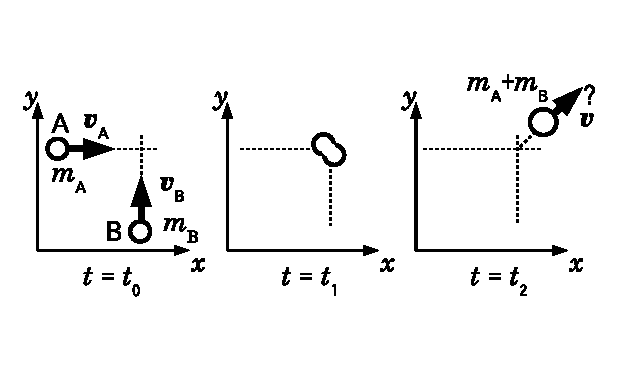
\includegraphics[width=7.0cm]{collision.eps}
    \caption{2つの質点の衝突合体}\label{fig:collision}
\end{figure}

極微の世界や高速の世界を除けば, どんな運動も運動方程式に従うので, 
この件も運動方程式を解けば完璧に予測・解明できるはずだ。
しかし, この件に関しては, 運動方程式を正面から解くのは難しい。
というのも, そもそも「衝突して合体」は, 時刻$t_1$の「瞬間」で起きるのではなく, 
衝突が始まって物体が徐々につぶれて, その間, 弾性力や摩擦力が
複雑に働き, やがてお互いがくっつきあって一体化するまで, 短い時間
だが複雑な現象が起きるのだ。その各時刻に, 2つの物体の間に
どのように力が働くのかを解明するのは大変難しい作業だ。

というわけで, この時刻$t_1$付近で起きる「衝突して合体」という複雑な
現象を運動方程式で直接扱うことは避けたい。君子危うきに近寄らず, 
と言うではないか。\mv

そこで有用なのが, これから学ぶ, 以下の法則である:
\begin{itembox}{運動量保存則}
外力が働かない系では, 全運動量(各質点の運動量の総和)は不変である。
\end{itembox}
外力とは, 考察の対象になっている物体どうしに働く力(それを内力という)
以外の力だ。本件でも外力は働いていない
\footnote{衝突して合体するまでに生じる複雑な力は, 
具体的にその力がどんなものなのかというのは置いといて, 
「考察の対象になっている物体どうしに働く力」なので内力である。}。
全運動量とは, 各物体の運動量の(ベクトルとしての)和である。
運動量とは, \eref{eq:def_momentum}で定義されたように, 質量と速度の積である。

この法則がなぜ成り立つかは, 後で説明するとして, とりあえずこの法則が正しいと
信じてみよう。本件では, 時刻$t_0$(つまり衝突前)の全運動量は, 
\begin{eqnarray} 
m_{\text A}{\bf v}_{\text A}+m_{\text B}{\bf v}_{\text B}\label{eq:momentum_mAmB_0}
\end{eqnarray} 
である。ここで, 添字のA, Bは, それぞれ質点A, 質点Bの属性であることを示す。
時刻$t_2$(つまり衝突後)では質点はひとつに合体しており, その運動量は, 
\begin{eqnarray} 
(m_{\text A}+m_{\text B}){\bf v}\label{eq:momentum_mAmB_1}
\end{eqnarray} 
である。運動量保存則は, \eref{eq:momentum_mAmB_0}と\eref{eq:momentum_mAmB_1}
が等しい, と主張するのだ。すなわち, 
\begin{eqnarray} 
m_{\text A}{\bf v}_{\text A}+m_{\text B}{\bf v}_{\text B}=(m_{\text A}+m_{\text B}){\bf v}
\end{eqnarray} 
が成り立つはずだ。それを認めるなら, 
\begin{eqnarray} 
{\bf v}=\frac{m_{\text A}{\bf v}_{\text A}+m_{\text B}{\bf v}_{\text B}}{m_{\text A}+m_{\text B}}\label{eq:2body_adhere}
\end{eqnarray} 
となって, 衝突後の質点の速度が求まる。実際, 実験してみると, 確かにこうなるのだ。\mv

%
\begin{q}\label{q:collision0}
図\ref{fig:collision}の問題において, $m_{\text A}=m_{\text B}=1.0$~kgとし, 時刻$t_0$でAは$x$軸
方向に1.0~m s$^{-1}$, Bは$y$軸方向に1.0~m s$^{-1}$で動いているとする。
\begin{enumerate}
\item 衝突合体後の速度${\bf v}$を求めよ。
\item $|{\bf v}|$を求めよ。
\end{enumerate}
\end{q}\mv

では, 運動量保存則を証明しよう。まず運動方程式に戻る(運動の話は全て運動方程式から始まるのだ!)。
質量$m$の質点が力${\bf F}$を受けて
運動しているとき, その運動は, どんなものでも以下の運動方程式に従う:
\begin{eqnarray}{\bf F}=m{\bf a}=m\frac{d{\bf v}}{dt}=m\frac{d^2{\bf r}}{dt^2}\end{eqnarray}
$t$は時刻である。${\bf r}, {\bf v}, {\bf a}$は
それぞれ, 質点の位置, 速度, 加速度。さて, 上の式は, 以下のように書ける:
\begin{eqnarray} 
m\frac{d{\bf v}}{dt}={\bf F}\label{eq:maF}
\end{eqnarray} 
両辺に$dt$をかけると次式になる:
\begin{eqnarray} 
m\,d{\bf v}={\bf F}\,dt\label{eq:consmom_mdv_Fdt}
\end{eqnarray} 
これを時刻$t=t_0$から時刻$t=t_1$まで$t$で積分すれば, 
\begin{eqnarray} 
\int_{{\bf v}(t_0)}^{{\bf v}(t_1)}m\,d{\bf v}=\int_{t_0}^{t_1}{\bf F}\,dt\label{eq:momentum_00}
\end{eqnarray} 
となる。左辺は, 
\begin{eqnarray} 
\Bigl[m{\bf v}\Bigr]_{{\bf v}(t_0)}^{{\bf v}(t_1)}=m{\bf v}(t_1)-m{\bf v}(t_0)
\end{eqnarray} 
となるから, \eref{eq:momentum_00}は, 
\begin{eqnarray} 
m{\bf v}(t_1)-m{\bf v}(t_0)=\int_{t_0}^{t_1}{\bf F}\,dt\label{eq:momentum1}
\end{eqnarray} 
となる。この式の左辺は「時刻$t_0$から$t_1$の間に運動量がどれだけ変わったか」だ。
一方, 右辺は\underline{力積}\index{りきせき@力積}(りきせき, と読む)と
いう量である。
\begin{itembox}{力積の定義}
時刻を$t$とする。質点に, 力${\bf F}(t)$が働くとき, 
\begin{eqnarray}
\int_{t_0}^{t_1}{\bf F}\,dt\label{eq:rikiseki}
\end{eqnarray}
を, 時刻$t_0$から$t_1$までに質点に働く力積と呼ぶ。
\end{itembox}

\begin{q}\label{q:def_rikiseki}
力積の定義を5回書いて記憶せよ。\end{q}\mv

すなわち, \eref{eq:momentum1}は, 「\textgt{運動量の変化は力積に等しい}」と解釈できる。これはこれで大切な法則である。そして, この法則をもとに, 運動量保存則が証明される(ちなみに, この法則のことを運動量保存則と呼ぶこともある)。

\begin{faq}{\small\textgt{「運動エネルギーの変化は仕事に等しい」という法則と似てますね}
... 似てるけど違います。両者の違いをきちんと認識しよう。運動エネルギーや仕事はスカラーで, その法則は運動方程式
を位置で積分して得られました。一方, 運動量や力積は\textgt{ベクトル}で, ここで述べた法則は
運動方程式を\textgt{時刻で}積分することで得られたのです。}\end{faq}\mv

さて, いま, A, Bという2つの質点が互いに力を及ぼしあいながら時刻$t=t_0$から時刻$t=t_1$まで
運動する状況を考えよう。
各質点は外力を受けることがないとする。
質点Aが質点Bから受ける力を${\bf F}_{\text {AB}}$, とし, 
質点Bが質点Aから受ける力を${\bf F}_{\text {BA}}$とする。それぞれの質点に関して, \eref{eq:momentum1}
と同様の式が成り立つはずである:
\begin{eqnarray}
&&m_{\text A}{\bf v}_{\text A}(t_1)-m_{\text A}{\bf v}_{\text A}(t_0)=\int_{t_0}^{t_1}{\bf F}_{\text {AB}}dt\label{eq:momentumA}\\
&&m_{\text B}{\bf v}_{\text B}(t_1)-m_{\text B}{\bf v}_{\text B}(t_0)=\int_{t_0}^{t_1}{\bf F}_{\text {BA}}dt\label{eq:momentumB}
\end{eqnarray}
これらを辺々足し合わせると, 
\begin{eqnarray}
&&m_{\text A}{\bf v}_{\text A}(t_1)-m_{\text A}{\bf v}_{\text A}(t_0)+m_{\text B}{\bf v}_{\text B}(t_1)-m_{\text B}{\bf v}_{\text B}(t_0)\nonumber\\
&&=\int_{t_0}^{t_1}{\bf F}_{\text {AB}}dt+\int_{t_0}^{t_1}{\bf F}_{\text {BA}}dt\nonumber\\
&&=\int_{t_0}^{t_1}({\bf F}_{\text {AB}}+{\bf F}_{\text {BA}})\,dt\label{eq:momentumABsum}
\end{eqnarray}
となる。ここで作用反作用の法則から, 
\begin{eqnarray} 
{\bf F}_{\text {AB}}=-{\bf F}_{\text {BA}}
\end{eqnarray} 
である。従って, 
\begin{eqnarray} 
{\bf F}_{\text {AB}}+{\bf F}_{\text {BA}}={\bf 0}
\end{eqnarray}
である。従って, \eref{eq:momentumABsum}の最後の行は${\bf 0}$になる(${\bf 0}$の積分は${\bf 0}$)。従って, 
\begin{eqnarray*} 
m_{\text A}{\bf v}_{\text A}(t_1)-m_{\text A}{\bf v}_{\text A}(t_0)+m_{\text B}{\bf v}_{\text B}(t_1)-m_{\text B}{\bf v}_{\text B}(t_0)={\bf 0}
\end{eqnarray*}
となる。書き換えれば, 
\begin{eqnarray} 
m_{\text A}{\bf v}_{\text A}(t_1)+m_{\text B}{\bf v}_{\text B}(t_1)\nonumber\\
=m_{\text A}{\bf v}_{\text A}(t_0)+m_{\text B}{\bf v}_{\text B}(t_0)\label{eq:consmom000}
\end{eqnarray} 
となる。この式は, 2つの質点の運動量の和は時刻$t_1$と時刻$t_0$で変わらない, ということだ。
以上から, 「2つの質点が, 外力の影響を受けずに運動する場合, 全運動量は不変である」ということ
が示された。次の問で証明するように, 質点が3つになっても, 同様の式が成り立つ。この証明を, 
任意の個数の質点に拡張することも容易にできる。つまり, 前述の運動量保存則が成り立つ!

%
\begin{q}\label{q:3body_momentum}
3つの質点A, B, Cが互いに内力のみを受けて運動する系でも, 全運動量が保存する
ことを示せ。ヒント:式(\ref{eq:momentumA})のような式を, A, B, Cのそれぞれに
ついて考え, 足し合わせればよい。ただし, Aに働く力は${\bf F}_{\text {AB}}+{\bf F}_{\text {AC}}$
であることに注意。
\end{q}

\begin{q} 2つの質点A, Bが, $x$軸上を互いに逆向きに等速直線運動で運動し, 接近し, 
いずれ衝突する。質点A, Bの質量はそれぞれ2.0~kgと3.0~kgであり, 
衝突前の質点A, Bの速度はそれぞれ$-4.0$~m~s$^{-1}$, $5.0$~m~s$^{-1}$である。
衝突後, 2つの質点はくっついて1つの質点になる場合, 衝突後のこの質点の速度を求めよ。\end{q}
\hv


\section{衝突のときエネルギーはどうなるのか?}

この「運動量保存則」は, 前章までに学んだ「力学的エネルギー保存則」になんとなく似ているが, 
正直なところ, どう違うのだろうか? そこで, 以下の問を考えよう:

%
\begin{q}\label{q:collision1}
問\ref{q:collision0}の続きを考える。
\begin{enumerate}
\item 衝突前の運動エネルギーの総和を求めよ。
\item 衝突合体後の運動エネルギーを求めよ。
\end{enumerate}
\end{q}

この現象では, 衝突合体で運動エネルギーが減ってしまった。では, この減ったぶん
のエネルギーはどこに行ってしまったのだろう?

まず考えられるのは, ポテンシャルエネルギーである。既に学んだ「力学的エネルギー
保存則」では, 運動エネルギーとポテンシャルエネルギーの総和は一定なのだから, 
運動エネルギーが減った分, ポテンシャルエネルギーが増えていれば, つじつまは合う。

しかし! この衝突ではポテンシャルエネルギーは変化していない。ていうか, 外力が
無いからそもそもポテンシャルエネルギーは0である。もし外力(ボールの衝突における重力など)
があったらどうだろう? 外力が仕事をすれば, それはポテンシャル
エネルギーを変化させるだろう。ところが, 衝突の短い瞬間だけに注目すると, 
物体の運動は小さい空間領域で発生するので, たとえ外力があっても, 外力に
よる仕事はほとんど無視できる(仕事=力$\times$変位の「変位」が小さいから!)。
従って, 外力がある場合でも, 衝突の前後で外力によるポテンシャルエネルギー
の変化はほぼ0だ。従って, 外力があろうがなかろうが, 衝突の前後でポテンシャル
エネルギーは変化しない。

ならば外力以外の力によるポテンシャルエネルギーはどうだろう? 例えば, ボールどうし
が衝突するとき, ボールは変形する。その変形は, ボールを構成する各部分の弾性力
に逆らって行われる(仕事がされる)ものなので, 弾性力によるポテンシャルエネルギーを
増加させる。しかもこの変形は, 衝突終了後も, ボールをぐにゃぐにゃと振動させる
ことによって継続する。弾性力によるポテンシャルエネルギーは, この振動の運動エネルギー
にも転化するだろう。

そのような振動は, やがて収まるだろう。それは, ボール内部の摩擦によるものである。
そのとき, 振動のエネルギーは, 最終的にはボールの温度を上げる熱エネルギーと
なるだろう。

このように, 衝突の際に減った運動エネルギーは, 物体内部の振動のエネルギーや熱
になるのである。\\

このようなことのない衝突, すなわち, 衝突によって全運動エネルギーが変化しない
(減らない)ような衝突を, \underline{弾性衝突}\index{だんせいしょうとつ@弾性衝突}とか, 
完全弾性衝突という。弾性衝突でない衝突現象(全運動エネルギーが減る衝突)を, 
\underline{非弾性衝突}という。上の例は, 非弾性衝突である。
\mv

\begin{freqmiss}{\small\textgt{弾性衝突を「エネルギーが失われない衝突」という}
... 弾性衝突でも非弾性衝突でも, 熱エネルギーまで含めて全てのエネルギーを
考えれば, エネルギーは失われません。どういう形のエネルギーについて話をして
いるのかに注意することが必要です。}\end{freqmiss}

\begin{freqmiss}{\small\textgt{弾性衝突を「運動量が失われない衝突」という}
... 弾性衝突でも非弾性衝突でも, 運動量は変化しません。それは\eref{eq:consmom000}
であなた自身が証明したことです。}\end{freqmiss}

\begin{q}\label{q:elastic_collision} 
\begin{enumerate}
\item 弾性衝突とは何か?
\end{enumerate}
\end{q}
\mv

%
%\begin{q}\label{q:collision2}
%$x$軸上に質量$m_{\text A}$の質点Aが静止している。ここに, $x$軸の負のほうから, 
%質量$m_{\text B}$の質点Bが速度$v$で正の方向に進んで来て, 質点$A$に弾性衝突した。衝突後の
%質点A, Bの速度をそれぞれ$v_{\text A}$, $v_{\text B}$とする。運動はすべて$x$軸の上で起きるとする。
%\begin{enumerate}
%\item 運動量保存則と力学的エネルギー保存則より, 以下の2つの式が成り立つことを示せ:
%\begin{eqnarray}
%&&m_{\text B}v=m_{\text A}v_{\text A}+m_{\text B}v_{\text B}\\
%&&\frac{1}{2}m_{\text B}v^2=\frac{1}{2}m_{\text A}v_{\text A}^2+\frac{1}{2}m_{\text B}v_{\text B}^2
%\end{eqnarray}
%\item これらの式から以下の式を得ることを示せ:
%\begin{eqnarray}
%v_{\text A}&=&\frac{2m_{\text B}}{m_{\text A}+m_{\text B}}\,v\label{eq:collision25}\\
%v_{\text B}&=&\frac{m_{\text B}-m_{\text A}}{m_{\text A}+m_{\text B}}\,v\label{eq:collision26}
%\end{eqnarray}
%\item もし, 2つの質点の質量が等しかったら, どういう現象が起きるか? 
%\item もし, 質点Aが質点Bよりはるかに重ければ, どういう現象が起きるか? 
%\item もし, 質点Aが質点Bよりはるかに軽ければ, どういう現象が起きるか? 
%\end{enumerate}
%\end{q}

\begin{figure}[h]
    \centering
    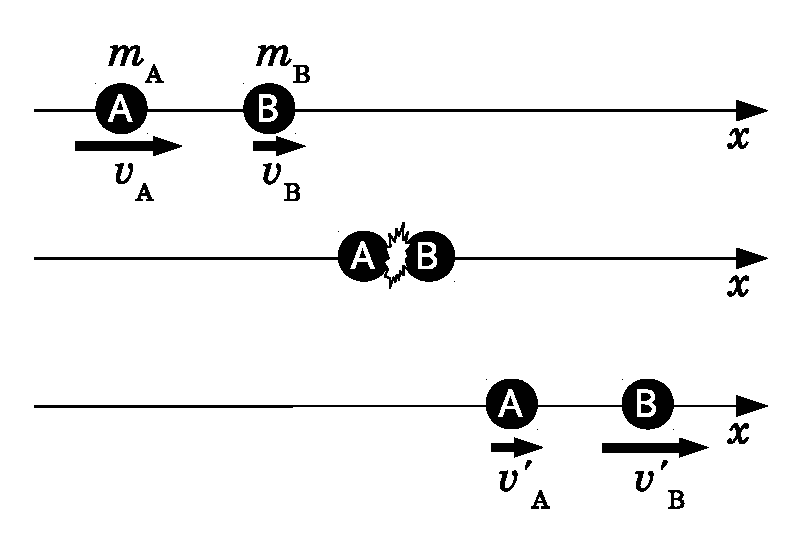
\includegraphics[width=6.5cm]{collision2.eps}
    \caption{1直線上を運動する2つの質点どうしの衝突。上: 衝突前, 中: 衝突の瞬間, 下: 衝突後}\label{fig:collision2}
\end{figure}

\begin{q}\label{q:collision2}
$x$軸上で, 2つの質点A, Bが, それぞれ速度$v_{\text{A}}$, $v_{\text{B}}$
で運動し(図\ref{fig:collision2}上), やがて互いに弾性衝突を起こし(図\ref{fig:collision2}中), 
衝突後はそれぞれ速度$v'_{\text{A}}$, $v'_{\text{B}}$で(ここではダッシュ'は微分ではなく, 
「衝突後」を表すしるし), 再び$x$軸上で運動をする
(図\ref{fig:collision2}下)。質点A, Bのそれぞれの質量を$m_{\text{A}}$, $m_{\text{B}}$とする。
2つの質点に外力は働いておらず, 2つの質点どうしに働く力(内力)は衝突時だけに働くとする。

\begin{enumerate}
\item 運動量保存則と力学的エネルギー保存則より, 以下の2つの式が成り立つことを示せ:
\begin{eqnarray}
&&m_{\text A}v_{\text A}+m_{\text B}v_{\text B}=m_{\text A}v'_{\text A}+m_{\text B}v'_{\text B}\label{eq:collision2_03}\\
&&\frac{1}{2}m_{\text A}v_{\text A}^2+\frac{1}{2}m_{\text B}v_{\text B}^2
=\frac{1}{2}m_{\text A}{v'_{\text A}}^2+\frac{1}{2}m_{\text B}{v'_{\text B}}^2\quad\quad\quad\label{eq:collision2_05}
\end{eqnarray}
\item \eref{eq:collision2_03}, \eref{eq:collision2_05}から次式を示せ:
\begin{eqnarray}
&&m_{\text A}(v'_{\text A}-v_{\text A})=-m_{\text B}(v'_{\text B}-v_{\text B})\label{eq:collision2_07}\\
&&m_{\text A}({v'_{\text A}}^2-v_{\text A}^2)=-m_{\text B}({v'_{\text B}}^2-v_{\text B}^2)\label{eq:collision2_09}
\end{eqnarray}
\item \eref{eq:collision2_09}から次式を示せ:
\begin{eqnarray}
&&m_{\text A}(v'_{\text A}-v_{\text A})(v'_{\text A}+v_{\text A})=-m_{\text B}(v'_{\text B}-v_{\text B})(v'_{\text B}+v_{\text B})\nonumber\\\label{eq:collision2_11}
\end{eqnarray}
\item \eref{eq:collision2_11}の両辺を\eref{eq:collision2_07}で割って次式を示せ:
\begin{eqnarray}
v'_{\text A}+v_{\text A}=v'_{\text B}+v_{\text B}\label{eq:collision2_13}
\end{eqnarray}
\item \eref{eq:collision2_13}を変形して次式を示せ:
\begin{eqnarray}
v'_{\text B}-v'_{\text A}=-(v_{\text B}-v_{\text A})\label{eq:collision2_14}
\end{eqnarray}
\item \eref{eq:collision2_14}を変形して次式を示せ:
\begin{eqnarray}
\frac{|v'_{\text B}-v'_{\text A}|}{|v_{\text B}-v_{\text A}|}=1\label{eq:collision2_145}
\end{eqnarray}
\end{enumerate}
\end{q}\mv\mv

\eref{eq:collision2_14}によって, ぶつかる前後で相対速度は, 向きが逆になることがわかった。
つまり, ぶつかる前には互いに近づいて来たが, ぶつかった後では互いに遠ざかっていく。これは
直感的にも明らかだ。

ぶつかった後の相対速度の大きさ$|v'_{\text B}-v'_{\text A}|$を, ぶつかる前の
相対速度の大きさ$|v_{\text B}-v_{\text A}|$で割ったものを
\underline{反発係数}\index{はんぱつけいすう@反発係数}とか跳ね返り係数と呼び, 慣習的には$e$と表す。すなわち, 
\begin{eqnarray}
e=\frac{|v'_{\text B}-v'_{\text A}|}{|v_{\text B}-v_{\text A}|}\label{eq:collision_coeff}
\end{eqnarray}
である。弾性衝突では, 
\eref{eq:collision2_145}からわかるように, $e=1$である。非弾性衝突では, 
$e$は0から1の間の値をとる。$e=0$は, 物体Bが物体Aにべちゃっとくっついてしまう場合だ。
例えばゴルフボールとゴルフクラブの衝突に関する反発係数は0.8程度である。\mv

\begin{faq}{\small\textgt{$e$って, ネイピア数(自然対数の底)じゃないんですか?}
... 記号がかぶってて, 紛らわしいけど, ここでは違います。$e$は反発係数で, 
0から1までの間の値をとります。ネイピア数は$e=2.718\cdots$だもんね。}\end{faq}\mv

\begin{q}\label{q:collision2_contin} 問\ref{q:collision2}の続きを考える。
\begin{enumerate}
\item \eref{eq:collision2_13}を使って, \eref{eq:collision2_07}から$v'_{\text B}$を消去することによって次式を示せ:
\begin{eqnarray}
v'_{\text A}=\frac{m_{\text A}-m_{\text B}}{m_{\text A}+m_{\text B}}v_{\text A}+\frac{2m_{\text B}}{m_{\text A}+m_{\text B}}v_{\text B}\label{eq:collision2_15}
\end{eqnarray}
\item \eref{eq:collision2_13}を使って, \eref{eq:collision2_07}から$v'_{\text A}$を消去することによって次式を示せ:
\begin{eqnarray}
v'_{\text B}=\frac{m_{\text B}-m_{\text A}}{m_{\text A}+m_{\text B}}v_{\text B}+\frac{2m_{\text A}}{m_{\text A}+m_{\text B}}v_{\text A}\label{eq:collision2_17}
\end{eqnarray}
\item $m_{\text A}=m_{\text B}$のとき, 次式を示せ:
\begin{eqnarray}
&&v'_{\text A}=v_{\text B}\label{eq:collision2_21}\\
&&v'_{\text B}=v_{\text A}\label{eq:collision2_23}
\end{eqnarray}
\item $m_{\text A}>>m_{\text B}$のとき, 次式を示せ:
\begin{eqnarray}
&&v'_{\text A}\fallingdotseq v_{\text A}\label{eq:collision2_25}\\
&&v'_{\text B}\fallingdotseq -v_{\text B}+2v_{\text A}\label{eq:collision2_27}
\end{eqnarray}
\end{enumerate}
\end{q}
\vspace{0.2cm}

\eref{eq:collision2_21}, \eref{eq:collision2_23}から, 
2つの質点の質量が等しければ, 弾性衝突によって速度が入れ替わる(図\ref{fig:collision24}), 
ということがわかった。追いついた方は追いつかれた方の速度になり, 追いつかれた方は
追いついた方の速度になる。
\begin{figure}[h]
    \centering
    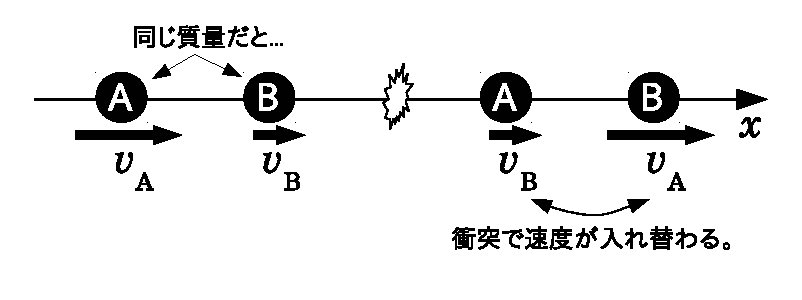
\includegraphics[width=6.5cm]{collision24.eps}
    \caption{1直線上を等速直線運動する2つの質点どうしの衝突。質量が等しく, なおかつ弾性衝突なら, 速度が入れ替わる。}\label{fig:collision24}
\end{figure}
この極端な場合は, 片方が静止してもう片方が
ぶつかってくる場合だ。ぶつかってきた方は衝突後に静止し, ぶつかられた
方がすっとんでいく。ビリヤードの経験がある人は, それを知っているだろう。\mv

ところで, \eref{eq:collision2_25}, \eref{eq:collision2_27}から, 片方の
質量が極端に大きいときは, 大きい方はほとんど速度を変えず(痛くも痒くもない), 
小さい方は激しく速度を変える(ふっとばされる), ということが
わかった(図\ref{fig:collision26})。小さな軽自動車と大きなトラックの衝突事故で, 
軽自動車に乗っていた人の方がダメージが大きいのはそのためだ。

\begin{figure}[h]
    \centering
    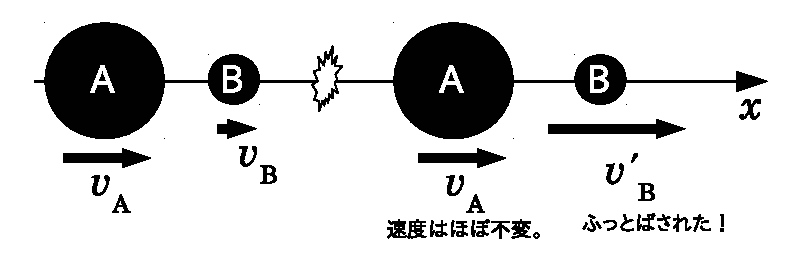
\includegraphics[width=6.5cm]{collision26.eps}
    \caption{1直線上を等速直線運動する2つの質点どうしの衝突。片方が極端に大きいときは, 小さいほうがふっとばされる。}\label{fig:collision26}
\end{figure}

%
\begin{q}\label{q:ball_bound}
ボールを高さ$h_0$から初速度0で真下に落として, バウンドさせる。
ボールと地面の間の反発係数を$e$としよう。空気抵抗やボールの回転は無視する。
\begin{enumerate}
\item ボールが地面につく直前の速度を$v_0$とする。力学的エネルギー保存則から次式を示せ:
\begin{eqnarray}v_0^2=2gh_0\label{eq:ball_bound1}\end{eqnarray}
\item ボールが地面で跳ね返った直後の速度を$v_1$とする。次式を示せ:
\begin{eqnarray}|v_1|=e|v_0|\label{eq:ball_bound2}\end{eqnarray}
\item ボールは地面で跳ね返ったあと上向きに運動し, いずれある点(それを到達点と呼ぼう)
に達してまた落ち始める。そのときの到達点の高さを$h_1$として, 次式を示せ:
\begin{eqnarray}v_1^2=2gh_1\label{eq:ball_bound3}\end{eqnarray}
\item 次式を示せ:
\begin{eqnarray}h_1=e^2h_0\label{eq:ball_bound4}\end{eqnarray}
\item そのまま放っておけば, またボールは地面に衝突して跳ね返り, また落ちて地面に衝突して
跳ね返り, ...ということを繰り返すだろう。$n$を1以上の整数として, ボールが$n$回バウンド
したあとの到達点の高さを$h_n$とすると, 次式を示せ:
\begin{eqnarray}h_n=e^{2n}h_0\label{eq:ball_bound5}\end{eqnarray}
\item $e=0.8$, $h_0=10$~mのとき, 到達点の高さが0.1~m以下になるまでに, 何回バウンドするか? 
\end{enumerate}
\end{q}
\mv

\begin{q}\label{q:balls_bound}
2つのボールを, わずかに隙間をあけて縦に重ねて, 高さ$h$から(初速度0で)
真下の地面に落とし, バウンドさせる。下のボールを「ボールA」とし, 
その質量を$m_{\text A}$とする。上のボールを「ボールB」とし, 質量を$m_{\text B}$とする。
ボールBはボールAよりはるかに小さく, $m_{\text A}>>m_{\text B}$とする。ボールAと
地面の衝突や, ボールAとボールBの衝突は弾性衝突であるとする。
重力加速度を$g$とする。上向きに座標軸をとる。

\begin{figure}[h]
    \centering
    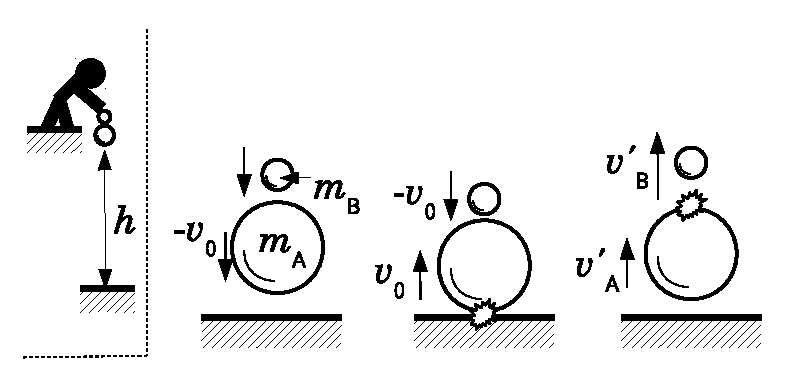
\includegraphics[width=7cm]{balls_bound.eps}
    \caption{2段のボールの落下と跳ね返り。問\ref{q:balls_bound}。}\label{fig:balls_bound}
\end{figure}

\begin{enumerate}
\item 地面に衝突する直前(図\ref{fig:balls_bound}中左)のボールAの速度の大きさを$v_0$とする。$v_0=\sqrt{2gh}$であることを示せ。
\item ボールAが地面に衝突して跳ね返った直後は, ボールBはまだボールAの上空にあるとする(図\ref{fig:balls_bound}中右)。このときのボールAの
速度を$v_{\text A}$, ボールBの速度を$v_{\text B}$とする。次式を示せ:
\begin{eqnarray}
&&v_{\text A}=v_0\\
&&v_{\text B}=-v_0
\end{eqnarray}
\item その直後に, ボールBはボールAに衝突して跳ね返る(図\ref{fig:balls_bound}右端)。衝突直後のボールBの速度を$v'_{\text B}$とする。
これらの一連の衝突は, 地面付近の狭い範囲で起きるので, 重力によるポテンシャルエネルギーの変化を
無視しよう。すると\eref{eq:collision2_27}が成り立つことから, 次式を示せ:
\begin{eqnarray}
v'_{\text B}\fallingdotseq 3v_0\label{eq:balls_bound4}
\end{eqnarray}
\item ボールBは, ボールAに衝突して跳ね返ったあと, もとの落下開始点(高さ$h$)の何倍の高さまで飛び上がるか?
\end{enumerate}
\end{q}
\mv

\section{回転運動再考}

ところで, 太陽のまわりを地球が円運動(公転)している系を考えよう。太陽と地球だけの系
には外力は働かないので, 運動量保存則から, 全運動量は一定のはずだ。さて, 地球の速度は, 
大きさこそ一定であっても, 円軌道に沿って時々刻々と向きを変える。すると, 地球の運動量は, 
大きさこそ一定であっても, 時々刻々と向きが変わるはずだ。一方, 太陽は静止しているから
運動量は無い。ということは, 全運動量は地球の運動量だけだ。ということは, 全運動量
が時々刻々と変化している, ということになる!! これは運動量保存則に矛盾している。どこが
間違っているだろうか?

実は, この考察は, 「太陽は静止しているから運動量は無い」から後が間違っている。
地球が太陽から引力を受けるように, 太陽も地球から引力を受ける(「作用・反作用の法則」)。
その力によって, 太陽も, 小さいながらも円運動するのだ。しかもその運動量は, 絶えず地球の運動量とは逆向きで
大きさが同じであるため, 太陽と地球の全運動量は0で一定なのである\footnote{ただし
太陽と地球の重心に対して静止している座標系で見た場合。}。
\hv



\begin{exq}\label{q:balls_bound_n} さっきは
ボールを2段にして落としたが, こんどはボールをもっとたくさん用意して重ねて
落としてみよう。$n$個のボールを縦に重ねて, 前問と同じように高さ$h$から
落とす。ボールは上のものほど軽く, 隣りあう上下のボールは, 上のボールのほうが
下のボールよりはるかに小さい(軽い)とする。最下部のボールが地面に弾性衝突して跳ね返ったあと, 
ボール同士は多段階に弾性衝突する(図\ref{fig:balls_bound_n})。最後に最上部のボールが跳ね上がるときのその
ボールの速度を$v'_n$とする。

\begin{figure}[h]
    \centering
    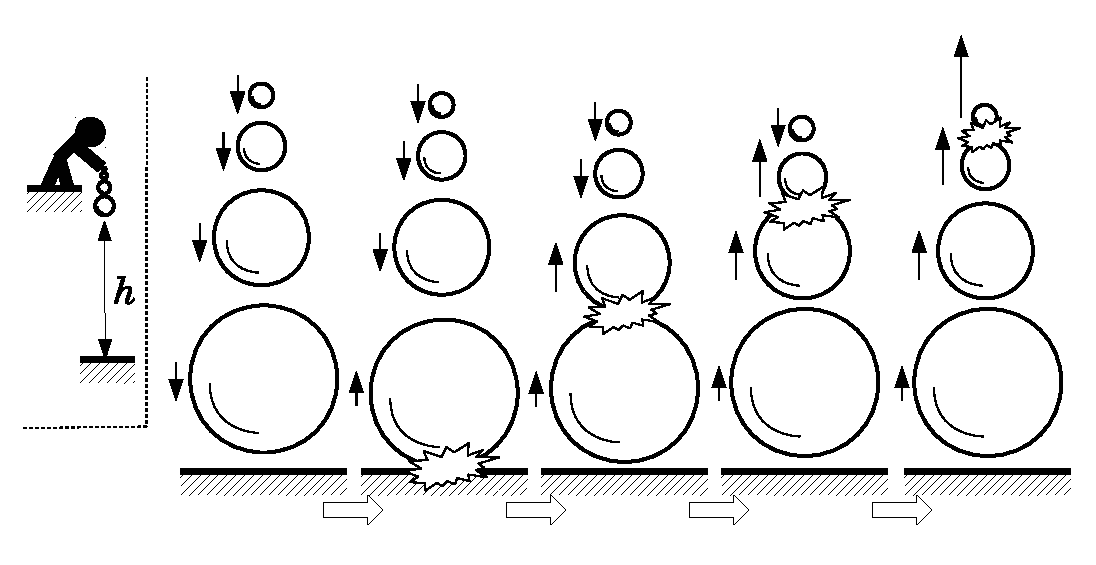
\includegraphics[width=7cm]{balls_bound_n.eps}
    \caption{多段のボールの落下と跳ね返り。問\ref{q:balls_bound_n}。}\label{fig:balls_bound_n}
\end{figure}

\begin{enumerate}
\item 次式を示せ:
\begin{eqnarray}
v'_n\fallingdotseq (2^n-1)v_0\label{eq:balls_bound_n3}
\end{eqnarray}
\item 最上部のボールは, もとの落下開始点(高さ$h$)の何倍の高さまで飛び上がるか?
\item ボール群を$h=5$~mから落下させ, 最上部のボールを宇宙の彼方まで
飛ばすには, ボールを10段程度にすればよいことを示せ。(ヒント: 第2宇宙速度)
\end{enumerate}
\end{exq}

\begin{exq} テニスのトップ選手の打つボールの速さは200~km/h程度である。
フェデラー選手が200~km/hのサービスを打ち, それを錦織圭選手が200~km/hで打ち返した。
その際, 錦織選手のラケットとボールが接触している時間は3.0~msだった。その間、
ボールに働いた力の大きさを見積もれ。また, そのような大きな力が発生するにもかかわらず, 
錦織選手の右腕が壊れないのはなぜだろう? ただしテニスボールの質量を60~gとする。\end{exq}

\begin{exq} 宇宙空間で直線上を加速しながら進むロケットの運動を考えよう。
ロケットにはたくさんの燃料が積まれている。燃料込みでのロケットの質量を$M$とする。
ロケットは, 相対速度$u$で, 燃料を後方に噴射することによって加速して
いく。と同時に, 噴射した燃料のぶんだけ質量$M$は減る。すなわち, ロケットは
質量が減るほど, 速度が増す。ロケットの初期速度を0, 初期の質量を$M_0$とする。
ロケットの速度$v$と質量$M$の関係を求めよ。ヒント: ある瞬間と, そこから少し経った
瞬間での, 運動量保存則を考える。ロケットの質量$M$は, $M+dM$に変わる($dM<0$)。
$dM$は出て行った微小な燃料の質量(にマイナスをつけたもの)。燃料は, $v-u$という速度で
ロケットから離れる。\end{exq}


\section{解答}
% $m_{\text A}=m_{\text B}=1$kgとし, 時刻$t_0$で$A$は$x$軸方向に1m/s, $B$は$y$軸方向に
\noindent{\textbf{答}}\ref{q:collision0}
\begin{enumerate}
\item $m_{\text A}=m_{\text B}=1$~kg, 
${\bf v}_{\text A}=(1\text{ m s}^{-1}, 0\text{ m s}^{-1})$, \\
${\bf v}_{\text B}=(0\text{ m s}^{-1}, 1\text{ m s}^{-1})$
として\eref{eq:2body_adhere}に代入すると, 
${\bf v}=(0.5\text{ m s}^{-1}, 0.5\text{ m s}^{-1})$。
\item $|{\bf v}|=|(0.5\text{ m s}^{-1}, 0.5\text{ m s}^{-1})|=0.71\text{ m s}^{-1}$。
\end{enumerate}

\noindent{\textbf{答}}\ref{q:def_rikiseki} 略。
\mv

% 3つの質点$A, B, C$が互いに内力のみを受けて運動する系でも, 全運動量が保存する
\noindent{\textbf{答}}\ref{q:3body_momentum}
(略証)
\begin{eqnarray*}
m_{\text A}{\bf v}_{\text A}(t_1)-m_{\text A}{\bf v}_{\text A}(t_0)=\int_{t_0}^{t_1}({\bf F}_{\text {AB}}+{\bf F}_{\text {AC}})dt\\
m_{\text B}{\bf v}_{\text B}(t_1)-m_{\text B}{\bf v}_{\text B}(t_0)=\int_{t_0}^{t_1}({\bf F}_{\text {BA}}+{\bf F}_{\text {BC}})dt\\
m_{\text C}{\bf v}_{\text C}(t_1)-m_{\text C}{\bf v}_{\text C}(t_0)=\int_{t_0}^{t_1}({\bf F}_{\text {CA}}+{\bf F}_{\text {CB}})dt
\end{eqnarray*}
これらの式を辺々加える。作用反作用の法則から${\bf F}_{\text {AB}}+{\bf F}_{\text {BA}}$
などは${\bf 0}$になるので, 結局, 
\begin{eqnarray*}
&&m_{\text A}{\bf v}_{\text A}(t_1)+m_{\text B}{\bf v}_{\text B}(t_1)+m_{\text C}{\bf v}_{\text C}(t_1)\\
&&=m_{\text A}{\bf v}_{\text A}(t_0)+m_{\text B}{\bf v}_{\text B}(t_0)+m_{\text C}{\bf v}_{\text C}(t_0)
\end{eqnarray*}

% 
\noindent{\textbf{答}}\ref{q:collision1}
\begin{enumerate}
\item $A, B$ともに同じ運動エネルギー: 0.5 Jをもつ。従って全運動エネルギーは, 1 J。
\item $(m_{\text A}+m_{\text B})|{\bf v}|^2/2=0.5$ J。
\end{enumerate}

% 弾性衝突とは何か? 
\noindent{\textbf{答}}\ref{q:elastic_collision}
衝突によって運動エネルギーが失われない衝突。

% $x$軸上に質量$m_{\text A}$の質点$A$が静止している。ここに, $x$軸の負のほうから, 
\noindent{\textbf{答}}\ref{q:collision2} 略。

\noindent{\textbf{答}}\ref{q:collision2_contin}
(1), (2), (3)は略(実直に計算すれば導出できる)。\mv
(4) \eref{eq:collision2_15}, \eref{eq:collision2_17}の分子分母を$m_{\text A}$で割ると, 
\begin{eqnarray*}
&&v'_{\text A}=\frac{1-m_{\text B}/m_{\text A}}{1+m_{\text B}/m_{\text A}}v_{\text A}+\frac{2m_{\text B}/m_{\text A}}{1+m_{\text B}/m_{\text A}}v_{\text B}\\
&&v'_{\text B}=\frac{m_{\text B}/m_{\text A}-1}{1+m_{\text B}/m_{\text A}}v_{\text B}+\frac{2}{1+m_{\text B}/m_{\text A}}v_{\text A}
\end{eqnarray*}
となる。ここで, $m_{\text A}>>m_{\text B}$なので, $m_{\text B}/m_{\text A}\fallingdotseq0$とすると, 上の2つの式は, 
\begin{eqnarray*}
&&v'_{\text A}\fallingdotseq \frac{1-0}{1+0}v_{\text A}+\frac{2\times0}{1+0}v_{\text B}=v_{\text A}\\
&&v'_{\text B}\fallingdotseq \frac{0-1}{1+0}v_{\text B}+\frac{2}{1+0}v_{\text A}=-v_{\text B}+2v_{\text A}
\end{eqnarray*}
となり, 与式を得る。
\vspace{0.2cm}


% ボールを高さ$h_1$から(初速度0で)真下に地面に落として, バウンドさせる。
\noindent{\textbf{答}}\ref{q:ball_bound}
\begin{enumerate}
\item 地面を基準点とする。ボールを手放した瞬間は, 重力によるボールのポテンシャルエネルギーは$mgh_0$で, 運動エネルギーは初速度0なので$0$。
従って力学的エネルギーは$mgh_0$。一方, 地面につく直前は, ボールのポテンシャルエネルギーは$0$で, 運動エネルギー
は$mv_0^2/2$。従って力学的エネルギーは$mv_0^2/2$。力学的エネルギー保存則より, $mgh_0=mv_0^2/2$。ここから与式を得る。
\item 略。($e$の定義から)
\item 略。(\eref{eq:ball_bound1}と同様)
\item 略。(\eref{eq:ball_bound1}, \eref{eq:ball_bound2}, \eref{eq:ball_bound3}より$v_0, v_1$を消去)
\item 前小問と同様に, $h_n=e^2h_{n-1}$。これは公比$e^2$の等比数列。従って与式を得る。(数学リメディアル教材参照)
\item $h_0=10$~mで, $h_n=e^{2n}h_0<0.1$~mより, \\
$e^{2n}<0.01$
となる。$e=0.8$だから, $0.8^{2n}<0.01$。$n=10$のとき
$0.8^{2n}=0.0115>0.01$。$n=11$のとき$0.8^{2n}=0.0074<0.01$。従って, $n=11$, つまり11回バウンドする。
\end{enumerate}
\vspace{0.2cm}


%
\noindent{\textbf{答}}\ref{q:balls_bound}
(1) ボールAについて, 落下から地面での衝突の直前までを考えると, 力学的エネルギー保存則より, 
\begin{eqnarray}
\frac{1}{2}m_{\text{A}}v_0^2=m_{\text{A}}gh\label{eq:balls_bound_ans2}
\end{eqnarray}
これを$v_0$について解けば与式を得る。\mv
(2), (3)は略(誘導に従って実直に計算すれば導出できる)。\mv
(4) ボールBについて, (1)と同様に考えれば, 次式のようになる: 
\begin{eqnarray}
\frac{1}{2}m_{\text{B}}v_0^2=m_{\text{B}}gh\label{eq:balls_bound_ans3}
\end{eqnarray}
一方, 最高到達点の高さを$H$とし, 衝突直後から最高点到達までを考えると, 力学的エネルギー保存則より, 
\begin{eqnarray*}
\frac{1}{2}m_{\text{B}}{v'_{\text B}}^2=m_{\text{B}}gH
\end{eqnarray*}
ここで(3)より, $v'_{\text B}=3v_0$だから, 
\begin{eqnarray}
\frac{9}{2}m_{\text{B}}v_0^2=m_{\text{B}}gH\label{eq:balls_bound_ans4}
\end{eqnarray}
となる。\eref{eq:balls_bound_ans4}の辺々を\eref{eq:balls_bound_ans3}の辺々で割ると, 
$9=H/h$となる。すなわち, $H=9h$。すなわち, もとの高さの9倍まで上がる。
\mv


\section{補遺: 量子のエネルギー}

実は, 我々が学んでいる力学(ニュートン力学)は, 分子や原子などの小ささになると, 
効力を失う。そのようなスケールを支配するのは, 「量子力学」という, 全く別な
理論だ。量子力学は物理現象や物理的存在の捉え方がニュートン力学とは
まるきり違っている。ニュートン力学では, 「速度」とか「力」とか
が大事な概念だったが, 量子力学では, それらにあまりこだわらない。というか, 
量子力学のスケールでは, そういうことにこだわっても仕方ないようなふうに
物体や現象が存在し, 振る舞うのである\footnote{量子力学では, 
速度のかわりに運動量, 力のかわりにポテンシャルエネルギーが, 
それぞれ重要な役割を担う。}。

それがどういうことなのかを理解するには, どうしても高度な数学が必要だ。
ある著名な物理学者は「神は非常に高度な数学者であり, 宇宙を作る時に
極めて高級な数学を使ったのだ」と言ったほどだ。我々は神様ほど高度な数学者では
ないのでどうしようもないが, それでも「化学II」「化学結合論」などの授業で
量子力学が出てくる。そこで, 量子力学のほんの入り口をここで学ぼう。
以下の話では, 「なぜそうなるのか」を説明することはできない。
自然はともかくそのように振る舞うのだ。

まず, 量子力学では, 物体や現象を「量子」という概念で把握する。電子や原子や
光は, いずれも「量子」として振る舞う。量子は, 1個2個と数えられるような
離散的な存在であり, その存在のあり方は, 「状態ベクトル」という数学的な
概念で表現される。その「ベクトル」という言葉から, 平面ベクトルや空間ベクトル
のようなもの, つまり「大きさと向きを持つもの」(矢印)を君は想像するかもしれないが, 
そうではない。状態ベクトルは, そういうベクトルとは違う, もっと抽象的な概念だ。
その「状態ベクトル」を, 位置$(x, y, z)$の関数として
表現したものを「波動関数」と言う\footnote{「ベクトル」が「関数」になる? どういうこと?
 と君は思うかもしれないが, 「関数もベクトルの一種だ」という話をどこかで
小耳に挟まなかっただろうか。}。波動関数は, 「シュレーディンガー方程式」
という小難しい微分方程式に従うことがわかっている。

量子が, ある特定のエネルギーを持つ状態にあるとき, 
シュレーディンガー方程式は「行列の固有値と固有ベクトル
を求める問題」(数学リメディアル教材でやった!)に帰着できる。
その「固有値」がエネルギーに該当し, 「固有ベクトル」が
状態ベクトル(それを位置で表現するならば波動関数と言っても
良い)に対応する(なのでそのような状態やそのエネルギーを
「固有状態」「固有エネルギー」と呼ぶ)。このとき, 状態ベクトル
は時刻$t$に対して振動的に依存する。その振動の角速度を
$\omega$とすると, 量子のエネルギー$E$は(それは行列の固有値
でもあるのだが), 
\begin{eqnarray}
E=\frac{h}{2\pi}\omega\label{eq:E_h_omega}
\end{eqnarray}
となる。ここで$h$は「プランク定数」と呼ばれる定数で, 
\begin{eqnarray}
h=6.626068\times10^{-34}\text{ J s}
\end{eqnarray}
である。$h/(2\pi)$は量子力学で頻繁にあらわれるので, $2\pi$をいちいち
書くのがめんどくさくなって, 物理学者達は, それを$\hbar$と
書き表すことにした(これを「エイチバー」と読む)。すなわち, 
\begin{eqnarray}
\hbar:=\frac{h}{2\pi}\quad\quad\text{(定義)}\label{eq:def_hbar}
\end{eqnarray}
である。すると, \eref{eq:E_h_omega}は次式のように書ける:
\begin{eqnarray}
E=\hbar \omega\label{eq:E_hbar_omega}
\end{eqnarray}

さて, 数学的な理由から, 波動関数は, 空間の中を振動しながら
広がっていくような性質を持つ。だから, 量子は「粒子の性質と
波の性質の両方を持つ」と言われることが多い。

特に, 光はそもそも電場と磁場の振動が空間を伝わる波なので, そのような
「波」のイメージが強い。実際, 光の状態ベクトル(波動関数)の振動の
角速度$\omega$は, 電場や磁場の振動の角速度$\omega$そのものである。
光速を$c$とすると, 波としての光は, 周期$2\pi/\omega$の間に速さ$c$で
波長$\lambda$だけ進むので, 
\begin{eqnarray}
\frac{2\pi}{\omega}\,c=\lambda
\end{eqnarray}
という式が成り立つ。この式を使って\eref{eq:E_h_omega}の$\omega$を消去
すると, 光の量子(それを光量子とか光子という)のエネルギーは, 
\begin{eqnarray}
E=\frac{hc}{\lambda}\label{eq:E_photon}
\end{eqnarray}
となる。この式はよく教科書に出てくるが, 注意すべきなのは, 
\underline{この\eref{eq:E_photon}は光子にしか成り立たない}, 
ということだ。光子以外にも, 様々な量子が世の中には存在し(電子とか), それぞれが波動関数の
角速度とか波長という特徴を持つのだが, \eref{eq:E_photon}は
必ずしも成り立たなくても, \eref{eq:E_h_omega}や\eref{eq:E_hbar_omega}
は光子も含めていかなる量子にも成り立つ。\mv

%2011.4.4 ヤマサキ この章は大きく変更した箇所はありません。
\chapter{熱力学入門}

熱力学は「化学I」や秋学期「物理学II」で学ぶ。しかし, 
それらは力学と多くの接点を持つので, ここで概略を学んでおこう。

\section{温度の定義}

物質や物体は, 膨大な数の原子や分子から構成される。
それらの粒子どうしは引力や斥力を及ぼしあい, 時には衝突しつつ
共存する。その様子を知るには, 原理的には全粒子のそれぞれに
ついて運動方程式を解いて追跡すればよい。そのように個々の
粒子の挙動に注目する観点を\underline{微視的}(ミクロ)な観点という。

しかし, 現実的にはそれは大変だし, そこまでのくわしい様子を知る
必要も少ない。むしろ, 興味があるのは, 粒子集団が, 全体として, 
平均的にどのような性質を持つか, ということだ。そのような
観点を\underline{巨視的}(マクロ)な観点という。

熱力学は, 物質や物体の巨視的な性質を検討する。そのときに最初に
便利な指標が\underline{温度}だ\index{おんど@温度}。温度とは何だろう?
温度には様々な定義があるが, わかりやすいのは以下である
\footnote{ここで温度を$T$と表すことに注意。これまでは$T$は
運動エネルギーを表していたが, 慣習的には温度を表す方が多い。
そこで, この章では運動エネルギーは$T$ではなく$K$で表す。}:

\begin{itembox}{絶対温度の定義 (エネルギー等分配則とも言う)}\label{def:temperature0}
物体を構成する粒子について, ひとつの粒子・ひとつの自由度における
平均的な運動エネルギー$K$が
\begin{eqnarray}K=\frac{1}{2}\,k_{\text{B}}T\label{eq:def_temperature0}\end{eqnarray}
と書けるとき, $T$をその物体の絶対温度と呼ぶ。
$k_{\text{B}}$は\underline{ボルツマン定数}\index{ぼるつまんていすう@ボルツマン定数}と呼ばれる定数で, 
\begin{eqnarray}
k_{\text{B}}=1.38065...\times10^{-23}\text{ J K}^{-1}\label{eq:def_Bolconst}
\end{eqnarray}
\end{itembox}
\eref{eq:def_temperature0}, \eref{eq:def_Bolconst}をもとに定義される温度の単位を, K(ケルビン)
という\footnote{温度の単位を表すKの記号は, 他の単位の記号と同じように, 
立体(正体)である。それに対して, \eref{eq:def_temperature0}の左辺に
出てくる, 運動エネルギーを表す変数$K$は, 斜体で書いていることに注意。これらは全く
別物だ。}。

ここで\underline{自由度}\index{じゆうど@自由度}とは, 独立した
「運動の仕方」の数である。例えば単原子分子からなる気体(図\ref{fig:deg_freedom1})では, 
ひとつの分子(=原子)は3つの各方向($x$方向, $y$方向, $z$方向)に
自由に直線運動ができ, 各方向の運動は互いに独立である($x$方向に
大きな速度で飛ぶからといって$y$方向にはゆっくり飛ばねばならない, というような
制約は存在しない)。従って, 自由度は3である。

\begin{figure}[h]
    \centering
    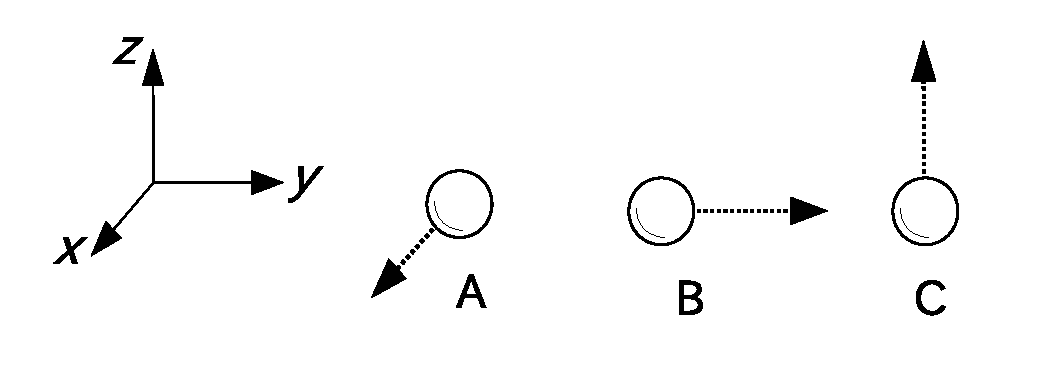
\includegraphics[width=8cm]{deg_freedom1.eps}
    \caption{単原子分子気体の自由度。A: $x$方向の直線運動, B: $y$方向の直線運動, C: $z$方向の直線運動。}\label{fig:deg_freedom1}
\end{figure}

\eref{eq:def_temperature0}は, 粒子の運動エネルギーが, 平均的には, 各自由度
に等しく割り当てられることも主張している。例えば, ある物質の中で, 多くの
粒子が同じ特定の方向にだけ激しく運動して, その方向の自由度だけに大きな運動エネルギー
を持つ, というような「偏った状態」にはならない, ということだ\footnote{それには
ちゃんとした理由があるのだが, 難しいのでここでは述べない。
興味ある人は, 「統計力学」という分野を勉強してみよう!}。その事情を表して, 
\eref{eq:def_temperature0}のことを\underline{エネルギー等分配則}
\index{えねるぎーとうぶんぱいそく@エネルギー等分配則}と呼ぶこともある。\mv

\eref{eq:def_temperature0}は「温度の定義」なので, とりあえずその由来や
正当性に疑問を持つ必要はない。むしろ不思議なのは, 
\eref{eq:def_temperature0}のように定義される温度が, 我々の感覚である
熱さ・冷たさや, 温度計の指す値にきちんと対応していることだ。そのあたり
は化学や物理学IIなどで学んでもらうとしよう。

\eref{eq:def_temperature0}は, 粒子の平均的な運動エネルギーは物体の
温度に比例することを主張している。その比例係数に「ボルツマン定数」という怪しげな
数とか「1/2」とかが現れているが, これらは「ケルビン」という「温度の単位」を人類が
採用してしまったことに対応するつじつま合わせ(単位換算)のための数に過ぎない。実際, 
運動エネルギーと温度が比例するのなら, いっそ(粒子の1自由度あたりの平均的な)
運動エネルギーそのものを温度としてしまえばよかったのだが, 今さらそれもめんどくさい
ので, 人類はこれからも, 温度とエネルギーを別の次元の物理量として扱っていくのだろう。\mv

\begin{q}\label{q:def_temperature}
絶対温度の定義を5回書いて記憶せよ。\end{q}\mv

\begin{q}\label{q:velocity_temperature}
質量$m$の気体分子の運動を考える。各分子が速度$(v_x, v_y, v_z)$で空間を飛ぶとき, 
エネルギー等分配則によって, $v_x$に関する運動エネルギー, つまり$mv_x^2/2$の平均は, $k_{\text{B}}T/2$
となる。従って, 平均的には\footnote{厳密には, $v_x$の二乗平均平方根(root-mean-square)。}
\begin{eqnarray}|v_x|=\sqrt{\frac{k_{\text{B}}T}{m}}\label{eq:velocity_temperature1}\end{eqnarray}
となる。$|v_y|$, $|v_z|$についても同様である。すると, 速度の大きさ(つまり速さ)$v$は, 
\begin{eqnarray}v=\sqrt{v_x^2+v_y^2+v_z^2}\label{eq:velocity_temperature2}\end{eqnarray}
なので, $v$は平均的には, 
\begin{eqnarray}v=\sqrt{3\frac{k_{\text{B}}T}{m}}\label{eq:velocity_temperature3}\end{eqnarray}
となる。以下, $T=300$ K(摂氏27度)で考える:
\begin{enumerate}
\item 水素分子H$_2$の$x$方向の平均的な速さを求めよ。
\item 水素分子H$_2$の平均的な速さを求めよ。
\item 窒素分子N$_2$の平均的な速さを求めよ。
\end{enumerate}
\end{q}

ところで, 「化学」で, 「グラハムの法則」\index{ぐらはむのほうそく@グラハムの法則}
というのを習った人もいるだろう。それは, 気体分子の速さ$v$が, 
その質量$m$の平方根に反比例する, という
法則だ。これは, \eref{eq:velocity_temperature3}で明らかだ。
\vspace{0.6cm}


\section{理想気体の状態方程式 (気体分子運動論)}

これまで学んだことを使って, 気体の温度・圧力・体積の間の関係を理論的に導いてみよう。

今, 簡単のため, 一辺の長さが$L$の立方体の箱を考える。
図\ref{fig:gas_motion}のように, 立方体の中心を原点Oとし, 
$x$, $y$, $z$軸のそれぞれに立方体の面が直交するように座標軸を設定する。
点$(L/2, 0, 0)$で$x$軸と直交する面を面Aと呼ぶ。
\begin{figure}[h]
    \centering
    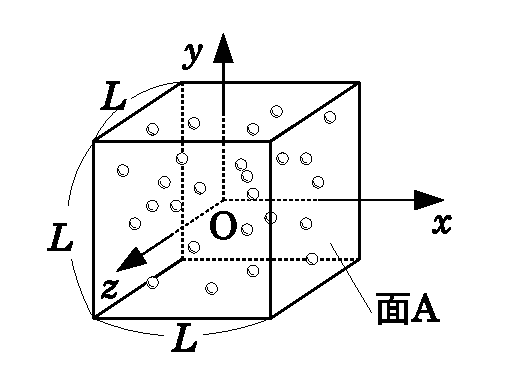
\includegraphics[width=8cm]{gas_motion.eps}
    \caption{気体分子の運動を考える座標系と箱。}\label{fig:gas_motion}
\end{figure}

この箱の中に, $N$個の気体分子が入っているとする。ここで, 以下の仮定を置く:
\begin{itembox}{理想気体の仮定}
\begin{itemize}
\item 気体分子の大きさは十分に小さい。
\item 気体分子同士に働く力は無視できる。
\end{itemize}
\end{itembox}
この2つの仮定を満たす分子からなる気体を「理想気体」という。
今, 立方体の中には理想気体が入っているとする。

箱の内側では気体分子が飛び交っており, 絶えずその一部が面Aに内側から衝突し, 
跳ね返されている。この衝撃が, 面Aを外に押し出そうとする。従って, それを打ち
消すように, 外側から適当な圧力($P$とする)をかけないと, この箱は壊れて
しまうだろう(図\ref{fig:gas_motionA})。

\begin{figure}[h]
    \centering
    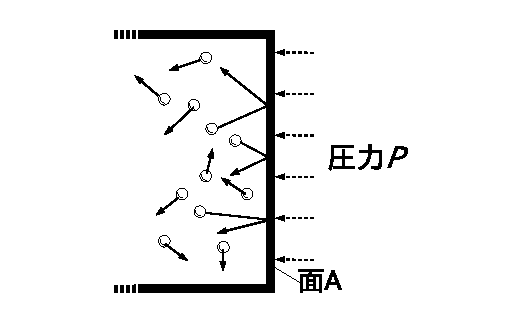
\includegraphics[width=8cm]{gas_motionA.eps}
    \caption{面Aの付近 ($z$軸の正の方向から見たところ)。分子が面Aにひっきりなしに
ぶつかるので, 面Aを外側から圧力$P$で支えていないといけない。}\label{fig:gas_motionA}
\end{figure}

その事情を詳しく見てみよう: 今, 簡単のために, どの気体分子も, $x$軸に沿った方向($x$軸の
正の方向か負の方向)に一定値$|v_x|$という速さで動いているとしよう。つまり, $x$軸方向の
速度は, $|v_x|$か$-|v_x|$であるとする(実際は気体分子の速度はもっといろんな可能性があり, 
$x$軸に沿った速度の二乗平均平方根が$|v_x|$に等しいだけだが, 仮にそういうのを考慮して厳密に理論展開
しても, 以下と同じ結論に至る)。従って, どの気体分子も, 時間$\Delta t$の間に, 
$|v_x| \Delta t$だけ$x$軸に沿って移動する。従って, 時間$\Delta t$の間に, 内側から面Aに
衝突する気体分子は, 面Aから距離$v_x \Delta t$までの領域にいるはずだ。その領域の体積は
\begin{eqnarray}L^2v_x\Delta t\label{eq:gas_stat_eq_0}\end{eqnarray}
である。箱の中の気体分子は均等に分布すると考えれば, 上述の領域の中の分子数は, 
領域の体積に比例するので, 
\begin{eqnarray}\frac{L^2v_x\Delta t}{L^3}N\label{eq:gas_stat_eq_1}\end{eqnarray}
となる\footnote{箱の体積は$L^3$であり, その中に$N$個の気体分子が均等に分布している。
従って, 箱の中の気体分子の数密度(単位体積当たりの分子数)は, $N/L^3$だ。これに, 
いま考えている領域の体積(\eref{eq:gas_stat_eq_0})をかければ, その領域内の気体分子数
が得られるはずだ。それが\eref{eq:gas_stat_eq_1}である。}。この個数のうち, 
半分が$x$軸の正方向, 半分が$x$軸の負の方向に進むので, 面Aに衝突する個数は, 
\begin{eqnarray}
\frac{1}{2}\frac{L^2v_x\Delta t}{L^3}N=\frac{Nv_x\Delta t}{2L}\label{fig:gas_motion_hitnum}
\end{eqnarray}
となる。

さて, 気体分子1個が面Aにぶつかって跳ね返る状況を考えよう。気体分子が跳ね返る時, 
面Aとの間に摩擦が働かず, 分子の運動エネルギーは変化しない(弾性衝突)とすると, 
面Aに平行な速度成分 ($v_y$と$v_z$) は変化せず, 面Aに垂直な成分($v_x$)が, 
大きさを変えずに符号だけ反転する。すると, $x$方向の運動量は, 
衝突前は$mv_x$, 衝突後は$-mv_x$になるので, 結局, 1個の気体分子の
衝突前後の運動量変化は次式になる:
\begin{eqnarray}
-mv_x-(mv_x)=-2mv_x\label{fig:gas_motion_changemom}
\end{eqnarray}

実際は1個でなく, \eref{fig:gas_motion_hitnum}で表される個数が$\Delta t$の
間に面Aにぶつかるので, それらの運動量変化の合計は次式になる:
\begin{eqnarray}
\frac{Nv_x\Delta t}{2L}\times(-2mv_x)=-\frac{Nmv_x^2\Delta t}{L}\label{eq:gas_motion_collide}
\end{eqnarray}
この運動量変化は, 面Aに外側からかかる力がもたらす力積に等しい
はずだ(運動量変化=加えられた力積)。

面にかかる力は, 圧力×面積であり, 面Aの面積は$L^2$だ。
従って, 面Aに(外側から)かかる力は$-PL^2$である(マイナスは, 力の向き, 
つまり$x$軸の負の方向を表すためにつけた)。その力による力積は, 
\begin{eqnarray}-PL^2\Delta t\label{eq:gas_motion_collide2}\end{eqnarray}
となる。\eref{eq:gas_motion_collide}と\eref{eq:gas_motion_collide2}が
一致することが, 面Aが静止する条件である:
\begin{eqnarray}-PL^2\Delta t=-\frac{Nmv_x^2\Delta t}{L}\end{eqnarray}
これを整理すると, 
\begin{eqnarray}PL^3=Nmv_x^2\label{eq:gas_stat_eq_5}\end{eqnarray}
となる。いま, $L^3$は箱の体積$V$なので, \eref{eq:gas_stat_eq_5}は
\begin{eqnarray}PV=Nmv_x^2\label{eq:gas_stat_eq_6}\end{eqnarray}
となる。さらに, \eref{eq:velocity_temperature1}より, 
\begin{eqnarray}v_x^2=\frac{k_{\text{B}}T}{m}\end{eqnarray}
なので, \eref{eq:gas_stat_eq_6}は, 以下のようになる:
\begin{itembox}{理想気体の状態方程式}
\begin{eqnarray}PV=Nk_{\text{B}}T\label{eq:gas_stat_eq_7}\end{eqnarray}
\end{itembox}

ここで, 分子数を「個」でなくて「モル」で数えよう。すなわち, $N$個が$n$モルに相当
するとすれば, $N=nN_\text{A}$である($N_\text{A}$はアボガドロ定数)。従って, \eref{eq:gas_stat_eq_7}は, 
\begin{eqnarray}PV=nN_\text{A}k_{\text{B}}T\label{eq:gas_stat_eq_72}\end{eqnarray}
となる。ここで, 物理学の慣習として, 以下の定数を導入する:
\begin{itembox}{気体定数の定義}
以下で定義される定数$R$を, 気体定数(gas constant)と呼ぶ:
\begin{eqnarray}R=N_\text{A}k_{\text{B}}\label{eq:def_gas_const}\end{eqnarray}
その値は, 8.314472... J~mol$^{-1}$K$^{-1}$である。
\end{itembox}
すると, \eref{eq:gas_stat_eq_72}は, 以下のように書ける:
\begin{itembox}{理想気体の状態方程式(モルで表す場合)}
\begin{eqnarray}PV=nRT\label{eq:gas_stat_eq_74}\end{eqnarray}
\end{itembox}

\begin{q}\label{q:def_ideal_gas}
理想気体とは何か?
\end{q}\mv

\begin{q}\label{q:ideal_gas_eq}
理想気体の状態方程式を導出せよ(上記の解説を整理して再現すればよい)。
\end{q}\mv

\begin{q}\label{q:tempera_kBR} 
\begin{enumerate}
\item ボルツマン定数$k_{\text B}$の値を, 有効数字3桁で述べよ。
\item 気体定数$R$の値を, 有効数字3桁で述べよ。
\item ボルツマン定数と気体定数の関係を, 式で述べよ。
\end{enumerate}\end{q}
\hv



\section{理想気体の内部エネルギーと温度}

さて, 物質や物体を構成する全ての粒子のエネルギー(運動エネルギーとポテンシャルエネルギー)を
合計したものを, その物質や物体の「内部エネルギー」という(定義)。ここで, 理想気体を考えよう。 
理想気体では, 気体分子が相互に及ぼす力は無視できるので, 気体分子同士が及ぼし合う力による
ポテンシャルエネルギーは無視してもかまわない。また, 非常な低温でもない限り, 重力による
ポテンシャルエネルギーは, 運動エネルギーよりはるかに小さい。従って, 
理想気体の内部エネルギーは, 大部分が構成粒子(気体分子)の運動エネルギーの総和であると
考えてよい\footnote{もし粒子が電離していたら, 電気的なポテンシャルエネルギーを持つ
かもしれないが, その場合は粒子同士の間にクーロン力が働くので, 理想気体の仮定に反する。
従って, 電気的なポテンシャルエネルギーも考えなくてよい。}。

エネルギー等分配則によれば, 運動エネルギーは1粒子あたり・1自由度あたり, 
平均的に$k_{\text{B}}T/2$だ。すると, 自由度$F$を持つ気体分子が$N$個からなる気体の内部エネルギー$U$
は\footnote{力学では, $U$は多くの場合, ポテンシャルエネルギーを表す記号として慣習的に使われる。
しかし, 熱力学では慣習的に$U$は内部エネルギーを表す。ここでは熱力学の慣習に従う。}, 
\begin{eqnarray}U=\frac{F}{2}Nk_{\text{B}}T\label{eq:gas_int_energy0}\end{eqnarray}
となる。すなわち, \underline{理想気体の内部エネルギーは}, \underline{温度に比例し, 
圧力や体積とは直接には無関係である}\footnote{もちろん, 圧力と体積は温度と関係があるから, 
圧力や体積は, 温度を介して間接的な関係はある。}。

さて, \eref{eq:gas_int_energy0}において分子が$n$モルあるとすると, $N=nN_{\text A}$だから, 
\begin{eqnarray}U=\frac{F}{2}nN_{\text A}k_{\text B}T\end{eqnarray}
となる。\eref{eq:def_gas_const}を使うと, 
\begin{eqnarray}U=\frac{F}{2}nRT\label{eq:gas_int_energy1}\end{eqnarray}
となる。特に, 分子数を1モルとすると, 
\begin{eqnarray}U=\frac{F}{2}RT\label{eq:gas_int_energy3}\end{eqnarray}
となる。

では, 自由度$F$はどう決まるのだろうか? 前述のように, 単原子分子気体(He, Ne等)は
3方向の直線運動の自由度を持つので$F=3$である。ところが, 2原子分子(H$_2$, O$_2$, N$_2$等)は
直線運動だけでなく, 回転運動も行う\footnote{回転運動にも運動エネルギーが
与えられることは, 後の章で学ぶ。}。直線状の棒を回すのには独立した(つまり互いに直交した)
軸が2つある\footnote{一般に, 物体を回転させる独立な回転軸は3つある。しかし, 
直線状の分子の場合は, 直線の断面は大きさを持たない点とみなしてよい。従って, 
直線を軸にする回転は考えなくてよい。同様に, 1原子分子は点とみなしてよいので, 
いずれの方向を軸とする回転も, 考えなくてよい。}ので, これらの回転の自由度は2である。
従って, これらの分子の自由度$F$は, 直線運動に3, 回転運動に2で, 合計5となる(図\ref{fig:deg_freedom2})。

\begin{figure}[h]
    \centering
    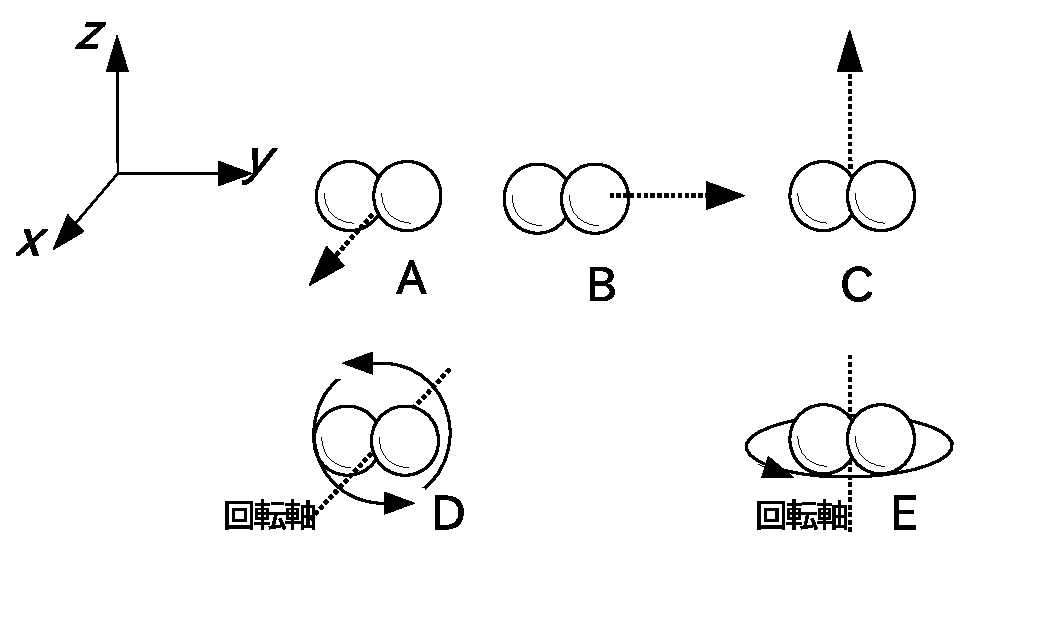
\includegraphics[width=8cm]{deg_freedom2.eps}
    \caption{2原子分子気体の自由度。A: $x$方向の直線運動, B: $y$方向の直線運動, C: $z$方向の直線運動, D: $x$軸まわりの回転運動, E: $z$軸まわりの回転運動。}\label{fig:deg_freedom2}
\end{figure}

従って, 理想気体1モルあたりの内部エネルギーは, 

\begin{eqnarray}
\text{単原子分子理想気体では, }U&=&\frac{3}{2}RT\label{eq:U_monomol}\\
\text{2原子分子理想気体では, }U&=&\frac{5}{2}RT\label{eq:U_2mol}
\end{eqnarray}
となる\footnote{高校で化学や物理学を学んだ人は, これは
「定積モル比熱」と「定圧モル比熱」の話か, と思うかもしれないが, そうではない。
その話はこの後に出てくる。}。

このように, 同じ温度, 同じモル数であっても, 分子が単原子分子か, 2原子分子かによって, 
内部エネルギーは違うのである。分子が複雑な運動をする可能性があるほど(つまり自由度が
大きいほど), 気体は大きな内部エネルギーを持つのである。
\footnote{理想気体では分子の大きさは無視できるはずなのに, 「2原子」分子を考える
のは変ではないか, と思う人もいるかもしれない。実は, 理想気体で「分子の大きさを無視する」
としたのは, 分子の大きさによって容器(分子が自由に飛び交うことのできる空間)の体積
が実質的に目減りするようなことがない, という意味だ。それに対して, 2原子分子を
考えるのは, 分子の回転運動が運動エネルギーを持つという性質を勘案するためであり, 
それは理想気体の仮定とは無関係である。}。

ただし, これらの式は(たとえ理想気体に対しても)厳密には成り立たない。特に, 低温になると, 
回転の自由度が意味を持たなくなる(自由度が減る)とか, 高温になると振動の自由度が
加わってくる(自由度が増える)などの, 不思議な現象が起きる。それらは量子力学を使わないと説明できない。\\



\section{比熱と熱容量}

ここで, 「熱容量」\index{ねつようりょう@熱容量}と「比熱」\index{ひねつ@比熱}
という概念を学ぼう。

ある物体の熱容量とは, その物体の温度を単位温度だけ上げるのに必要な熱量
のことである。すなわち, ある物体に熱量$dQ$を加えた時の温度の変化が
$dT$のとき, $dQ/dT$のことを熱容量と呼ぶ(定義)。熱容量は温度によって
変わることがあるので, この$dQ$や$dT$は, できるだけ小さい値(微小量)であるべきである。

単位量の物質の熱容量を「比熱」という。すなわち, ある物体の物質量が$X$であり, 
その物質に熱量$dQ$を加えた時の温度の変化が$dT$のとき, $dQ/(X\,dT)$の
ことを比熱と呼ぶ(定義)。特に, 物質量$X$を質量で表すときに「比熱」と呼び, 
物質量$X$をモルで表すときには「モル比熱」と呼ぶ。

熱容量は「物体」に関する量であり, 比熱は「物質」に関する量である。\\


\section{理想気体の定積モル比熱}

では, 理想気体の比熱について学ぼう。ここではモル比熱を考える。

気体に熱を加えたら, 普通, 気体はあたたまるだろう。しかし, 同時に, 気体は
膨張もする。このとき, 問\ref{q:gas_work}で見たように, 気体は仕事をする。
その仕事のぶんだけ, どこかからエネルギーが必要である(エネルギー保存則!)。
それは, 気体に加えられた熱かもしれないし, 気体がもともと持っていた内部エネルギー
かもしれない。

とりあえずそういう面倒なことを考えるのは避けたいので, 温めても気体は膨張しない
条件, すなわち気体をガッチリした容器に入れて体積が変わらないようにして温める
ことを考えよう。このように体積一定での変化を定積変化とか定積過程と呼ぶ。
定積変化でのモル比熱を「定積モル比熱」\index{ていせきもるひねつ@定積モル比熱}
と呼び, $C_{\text{v}}$と書く(添字のvは, volumeのv。volumeが変わらないよ, 
という意味)。

体積が変わらないなら, 加えた熱は全部内部エネルギーに変わる。$n$モルの理想気体の
内部エネルギー$U$は, \eref{eq:gas_int_energy1}より, 
\begin{eqnarray}
U=\frac{F}{2}nRT\label{eq:specific_heat_vconst2}
\end{eqnarray}
である。ここで熱量$dQ$を加えて温度が$dT$だけ上がったとすると, 内部エネルギーは$U+dQ$, 
温度は$T+dT$になるから, 
\begin{eqnarray}
U+dQ=\frac{F}{2}nR(T+dT)\label{eq:specific_heat_vconst4}
\end{eqnarray}
である。\eref{eq:specific_heat_vconst4}から\eref{eq:specific_heat_vconst2}を
辺々引くと, 
\begin{eqnarray}
dQ=\frac{F}{2}nR\,dT\label{eq:specific_heat_vconst6}
\end{eqnarray}
となる。従って, 定積モル比熱は, 
\begin{eqnarray}
C_{\text{v}}=\frac{dQ}{n\,dT}=\frac{F}{2}R\label{eq:gas_specificheat}
\end{eqnarray}
となる。特に, 
\begin{eqnarray}
\text{単原子分子理想気体では, }C_{\text{v}}&=&\frac{3}{2}R\label{eq:Cv_monomol}\\
\text{2原子分子理想気体では, }C_{\text{v}}&=&\frac{5}{2}R\label{eq:Cv_2mol}
\end{eqnarray}
である。そして, \eref{eq:gas_specificheat}と\eref{eq:gas_int_energy1}を見比べれば, 
\begin{eqnarray}
U=n\,C_{\text{v}}\,T\label{eq:U_nCvT}
\end{eqnarray}
であることがわかる。この式は, 明らかに, 定積変化という条件とは
無関係に成り立つ。つまり, 理想気体の内部エネルギーは, 一般的に, モル数と
定積モル比熱と絶対温度の積である。

では, 「体積一定」という条件を外したら, 理想気体のモル比熱はどうなるだろうか?
それを検討するには, 気体の内部エネルギーと熱と仕事について, ここで
しっかり考え方を固めておかねばならない。それが次節の内容である。\\



\section{熱力学第一法則}

我々は既に「力学的エネルギー保存則」を学んだが, エネルギーは, 
熱も含めて, より広い範囲で保存する(どこかに消えたりどこかから
湧いて出たりしない)。熱力学的には, 以下の法則である:
\begin{eqnarray}
\Delta U=Q+W\label{eq:thermlaw1}
\end{eqnarray}
ただし, $U$は系の内部エネルギー, $\Delta U$は内部エネルギーの
変化, $Q$は外から系に与えられた熱, $W$は外から系になされた
仕事である。これを「熱力学第一法則」\index{ねつりきがくだいいちほうそく@熱力学第一法則}
という。要するに「熱と仕事が与えられたぶんだけエネルギーが増える」
というわけだ。

\begin{q}\label{q:themlaw1} 熱力学第一法則を5回書いて記憶せよ。
「ただし書き」もちゃんと書くこと!\end{q}\mv

ここで, $\Delta U$は微小量でなくても構わない。普通, $\Delta$なんちゃら
というと, (有限な)微小量を考えることが多いが, 熱力学で出てくる
$\Delta$は「微小」ではない, 単なる「差」とか「変化」を表す。
微小を意味するときは, $\Delta$でなく$d$を使うことが多い。
微小量で\eref{eq:thermlaw1}を表現すると, 
\begin{eqnarray}
dU=dQ+dW\label{eq:thermlaw1inf}
\end{eqnarray}
となる($dQ$は外から系に加えられた微小な熱, $dW$は外から系になされた
微小な仕事)。ところが, \eref{eq:gas_work5}で学んだように, 気体の体積の微小な
変化$dV$に伴って, 系が外界からされる仕事は, 
\begin{eqnarray}dW=-P\,dV\end{eqnarray}
である。これを使うと上の式は, 
\begin{eqnarray}
dU=dQ-P\,dV\label{/eq:thermlaw1infPdV}
\end{eqnarray}
と書ける。これを変形すると, 次式になる: 
\begin{eqnarray}
dU+P\,dV=dQ\label{eq:thermlaw1infPdV2}
\end{eqnarray}
これは微小量での式だが, \textgt{もし圧力$P$が一定ならば}, 容易に
積分できて, 
\begin{eqnarray}
\Delta U+P\Delta V=Q\label{eq:thermlaw1infPdV3}
\end{eqnarray}
となる。


\section{理想気体の定圧モル比熱}

では, 「体積一定」という条件を外して, 理想気体のモル比熱を考えよう。
といっても, ここでは特に, 「圧力一定」という条件で考えよう。そのような条件での変化を
「定圧変化」とか「定圧過程」という。定圧過程でのモル比熱を「定圧モル比熱」
と呼び, $C_{\text{p}}$と表す。

$C_{\text{p}}$を求めるには, 熱力学第一法則から出発する。ここでは
\eref{eq:thermlaw1infPdV2}から出発しよう。この式の左右を入れ替え, 
\eref{eq:U_nCvT}を使えば, 
\begin{eqnarray}
dQ=nC_{\text{v}}dT+P\,dV
\end{eqnarray}
である。

ところで, 理想気体の状態方程式から, $PV=nRT$である。$P$と$n$は一定であり, 
$R$は定数なので, $P\,dV=nR\,dT$である。これを上の式に代入すれば, 
\begin{eqnarray}
dQ=nC_{\text{v}}dT+nR\,dT=n(C_{\text{v}}+R)\,dT
\end{eqnarray}
となる。従って, 
\begin{eqnarray}
C_{\text{p}}=\frac{dQ}{n\,dT}=C_{\text{v}}+R
\end{eqnarray}
である。つまり, 定圧モル比熱は, 定積モル比熱に気体定数を加えたものである。

\begin{q} 以下を示せ:
\begin{eqnarray}
\text{単原子分子理想気体では, }C_{\text{p}}&=&\frac{5}{2}R\label{eq:Cp_monomol}\\
\text{2原子分子理想気体では, }C_{\text{p}}&=&\frac{7}{2}R\label{eq:Cp_2mol}
\end{eqnarray}
\end{q}

\begin{faq}{\small\textgt{\eref{eq:thermlaw1infPdV3}が
ピンと来ません。「加えられた熱」$Q$が「内部エネルギーの変化」$\Delta U$に
等しいのはわかります。でも, 仕事$P\Delta V$というのがわかりません}
 ... では例を挙げましょう。純粋なエタノール(液体)と純水(液体)をまぜると, 
できた「エタノール水溶液」は暖かくなります(やったことがなければやってみて
ください!)。この熱はどこから来るのでしょう? エタノール分子は水分子と
引き合いますから, それらどうしがくっつくと(水和すると), 互いの引力
のポテンシャルエネルギーが, 熱として放出されるのです。これが
$\Delta U$にあたります。ここでは$U$は小さくなるので, $\Delta U$は
マイナスです。つまり, 系に熱を「加える」のではなく系から熱が「出る」のです。
だから温かくなるのです。

しかし! それだけではないのです! エタノール水溶液の体積は, 
元のエタノールの体積と水の体積を足したものよりも, わずかに小さく
なります。縮むのです! このとき, 体積が縮む分, 周囲の大気は水溶液
に対して仕事をします。それが$P\Delta V$です。ここでは$\Delta V$は
マイナスですので, $P\Delta V$もマイナスです。つまり, その仕事も
外に熱として出るのです。

従って, 水溶液が温かくなるのは, 分子同士の引力によるポテンシャルエネルギー
と, 水溶液の体積が小さくなることに伴う外部(大気)による仕事の両方
が寄与するのです。

このように, 反応熱を考えるには, 単に分子同士の引力や斥力だけでなく, 
まわりの環境からの仕事も考慮する必要があります。それをうまく整理して
くれるのが, 次節の「エンタルピー」です。}\end{faq}\mv


\section{エンタルピー}

生物資源学類では, 1年次「化学I」で, エンタルピーという概念を習う。
エンタルピーは, 化学反応や相変化を予測したり制御するのに必要な
概念であり, 特に, 「反応熱」に関わっている。

ところが, 多くの1年生は「エンタルピーって結局何?」と悩む。おまけに, 
そのあとに「エントロピー」という紛らわしい概念が出てきて混乱する。

\textgt{そのような悩みは, 定義を覚えていないことから発する}。
くどいようだが, まず定義をきちんと覚えないと何も話がはじまらない。
\begin{itembox}{エンタルピーの定義}
系の内部エネルギーを$U$, 圧力を$P$, 体積を$V$とすると, 
\begin{eqnarray}
H:=U+PV\label{eq:def_enthalpy}
\end{eqnarray}
をエンタルピーという(定義)。
\end{itembox}

\begin{q}\label{q:def_enthalpy} エンタルピーの定義を5回書いて記憶せよ。\end{q}\mv

さて, 定義を覚えたら, エンタルピーの意味を少しずつ考えていこう。
まず, この$H$の変化を考えてみよう。すなわち, ある状態(内部エネルギー
$U$, 圧力$P$, 体積$V$, エンタルピー$H$)から変化した状態
(内部エネルギー$U+\Delta U$, 圧力$P+\Delta P$, 体積$V+\Delta V$, エンタルピー$H+\Delta H$)
を考え, そのときのエンタルピーの変化を考えよう。変化前は, 
\begin{eqnarray}
H=U+PV
\end{eqnarray}
変化後は, 
\begin{eqnarray}
H+\Delta H=(U+\Delta U)+(P+\Delta P)(V+\Delta V)\nonumber\\
\end{eqnarray}
後者から前者を引くと, 
\begin{eqnarray}
\Delta H=\Delta U+P\Delta V+V\Delta P+\Delta P\Delta V\label{eq:enthalpy_change05}
\end{eqnarray}
となる。\textgt{もしこの変化が, 圧力は不変(一定)の状態で
行われたら}, $\Delta P=0$なので, 上の式は, 
\begin{eqnarray}
\Delta H=\Delta U+P\Delta V
\end{eqnarray}
となる。この右辺は\eref{eq:thermlaw1infPdV3}の左辺と同じだ。従って, 
\begin{eqnarray}
\Delta H=Q
\end{eqnarray}
となる。つまり, \textgt{定圧変化では, 系に加えられた熱量は, 
エンタルピーの変化(増加分)に等しい}。これがエンタルピーの「意味」だ。

\begin{faq}{\small\textgt{これがエンタルピーの意味だと言われても, 
ピンと来ません。なんで定圧に限定するのですか? それで何が嬉しいのですか? 
「系に加えられた熱量」がわかって何が嬉しいのですか?}
 ... まず, 世の中の現象の多く, 特に地上で起きる現象の多くは圧力
一定のもとで起きます。例えば君が料理を作る時, 圧力釜などを使わない
限り, 煮る・焼く・蒸す・混ぜる・凍らす・解凍するなどは, 一定の圧力(大気圧)
のもとで起きます。従って, 定圧を仮定しても, 理論の適用範囲はそんなには
限定されません。むしろ, 定圧を仮定することで, 現象の記述や解析は
単純になり, 楽になります。「系に加えられた熱量」は, 言葉を変えれば, 
「その変化を起こすのに外から加えねばならない必要な熱量」とも言えます。
また, これがマイナスの場合は, 「系から外に出る熱量」(要するに反応熱)
です。化学反応を制御したり, その反応熱を利用したりするとき, こういうのって, 
めっちゃ大事じゃないですか!}\end{faq}\mv


\section{エントロピー}

次に学ぶのは「エントロピー」である。エントロピーは, たくさんの分子や原子
からなる集団が, 全体としてどのように自発的にふるまうかを説明するときに
必要な概念である。

エントロピーはエンタルピーに名前が似ているので, 初学者は混同しやすいが, 
両者は全く異なる量である。名前が似ているのは偶然に過ぎない。そもそも名前が
似ているからといって、実体どうしも似ているとか互いに関係があるとはかぎらない。
例えば, 福井県の小浜市と米国元大統領のオバマ氏は名前が似ているが実体
は全く違う。エントロピーとエンタルピーもそういうものだと思っておけばよい。\\

まずエントロピーのその定義を述べよう。系には各状態において「エントロピー」
という量があり, 状態1のときのエントロピーを$S_1$, 状態2のときの
エントロピーを$S_2$とし, 
エントロピーの差, すなわち$S_2-S_1$を$\Delta S$とすれば, $\Delta S$は
次式を満たす, と約束する: 
\begin{eqnarray}
\Delta S=\int_{\text{状態1}}^{\text{状態2}} \frac{dQ_{\text{rev}}}{T}\label{eq:def_entropy}
\end{eqnarray}
ここで, 積分は, 系が状態1から状態2まで\textgt{可逆的に}変化したときに
関するものであり, $Q_{\text{rev}}$は外から系に\textgt{可逆的に}
与えられる熱量, $T$は絶対温度である。 これがエントロピーの定義である。
「可逆的」の意味は次節で述べる。

もし, 状態1と状態2が互いに非常に近い状態であるとき, すなわち変化の量が微小
であるとき, $\Delta S$は微小量$dS$と書くことができ, また, 微小変化の間で
温度$T$はほとんど変わらないと考えてよいので, 上の式は, 
\begin{eqnarray}
dS=\frac{dQ_{\text{rev}}}{T}\label{eq:def_entropy2}
\end{eqnarray}
と書いてもよい。

このように, エントロピーは, それ自体ではなく, その「変化」が先に定義される。

と言われても, 「わかりにくい!」というのが正直なところだろう。そう, エントロピー
は初学者にはなかなかわかりにくいのだ。諸君はまず, \eref{eq:def_entropy}, \eref{eq:def_entropy2}
をしっかり頭に叩き込もう。そして, それをもとに, いろんな話について行けば, 
次第にエントロピーが何なのか, わかってくるだろう。
\hv

\begin{q}\label{q:def_enthalpy} 上のエントロピーの
定義をそれぞれ5回書いて記憶せよ。\end{q}\mv


\section{可逆過程}

以後, 少しずつ, エントロピーの「意味」を理解していこう。

まず, エントロピーの定義で, 「可逆的に」\index{かぎゃくてき@可逆的}という
言葉が出てきた。これはとても大切なキーワードである。

ある系の状態が変化したとき, (その気になれば)変化後の状態から変化前の
状態に戻すことができ, しかも外部に何の影響も残さないようにそれができる
場合, そのような変化を「可逆的な変化」あるいは「可逆過程」という(定義)。

\begin{exmpl}\label{exmpl:lift_reverse} 物体を重力に逆らってゆっくり持ち上げるというのは可逆過程である。
持ち上げるときにエネルギー(=仕事=重さ×持ち上げた高さ)が必要だが, 
持ち上がった後に, 物体を元の高さまで戻すならば, 重力が仕事をして, 
持ち上げた時に使ったエネルギーを埋め合わす。\end{exmpl}

\begin{exmpl} ある速さで地面を滑っていた物体が, 地面との摩擦によって止まる, 
というのは可逆過程ではない。というのも, 物体が持っていた運動エネルギー
は摩擦によって熱エネルギーに変えられてしまう。この変えられた熱エネルギー
をもういちど集めて, 物体の運動エネルギーに変えて, 物体を滑らせるという
のは, どう考えても無理である。\end{exmpl}

熱力学では, 気体の状態変化がよく例に使われるので, 以後はそういう話に
絞ろう。\\

まず, 外部に熱が出入りしないように気体を圧縮させたり膨張させたりする過程, 
すなわち\textgt{断熱過程は, 可逆過程である}。なぜか? 
変化に必要なのは外部との仕事のやりとりだけである。
仕事は例\ref{exmpl:lift_reverse}のようにたくわえたり放出したりできるので, 
元に戻すときに, 外部に何も影響を残さない。

断熱変化におけるエントロピー(の変化)は? そもそも外から系には出入りしないので, 
\eref{eq:def_entropy}の$dQ_{\text{rev}}$はゼロである。従って, この積分も0であり, 
従って, エントロピーの変化も0である。要するに, \textgt{理想気体の
断熱変化ではエントロピーは変化しない}。\\

また, 系の温度が変わらない変化(等温変化)はどうだろうか?

\begin{exmpl}\label{exmpl:gas_expand_rev} 
ある気体を, 温度を一定に保ったまま, 体積を膨張または圧縮させることを考える。
このとき, その気体をピストンに入れたまま, 同じ温度を持つ大きな環境
(熱容量が無限に大きなもの, たとえば大きなお風呂)に浸して変化させる
ものとしよう。ゆっくり気体を膨張させたとき, 気体は環境に対して仕事をするが, 
それに必要な仕事と同じだけの熱が, 環境から気体に流れ込む。逆に, 
気体をゆっくり圧縮したときは, 環境は気体に仕事をするが, その仕事と
同じだけの熱が, 気体から環境に流れ出す。このように, 変化を元に戻すときに, 
外部(環境)に何も影響を残さない。従って, \textgt{理想気体の等温変化は
可逆過程である}。

このときのエントロピー(の変化)はどうなるだろう? 
まず, 熱力学第一法則から, 熱の出入りを見積もろう。\eref{eq:thermlaw1infPdV2}より, 
\begin{eqnarray}
dU+P\,dV=dQ
\end{eqnarray}
である。理想気体の内部エネルギー$U$は温度だけに依存し, 圧力$P$や体積$V$には無関係
なので, 等温変化の前後では$U$は変わらない。従って, $P\,dV=dQ$である。等温変化は
可逆的なので$dQ$は$dQ_{\text{rev}}$であり, \eref{eq:def_entropy}より, 
\begin{eqnarray}
\Delta S=\int_{\text{状態1}}^{\text{状態2}} \frac{dQ_{\text{rev}}}{T}=\int_{V_1}^{V_2}\frac{P\,dV}{T}
\end{eqnarray}
である。ここで, $V_1$と$V_2$は, それぞれ状態1 (最初の状態), 状態2 (膨張または圧縮が終わったときの状態)
のときの体積を意味する。理想気体の状態方程式から, $P=nRT/V$であるので($n$はモル数), 
\begin{eqnarray}
\Delta S=\int_{V_1}^{V_2} \frac{n\,R\,dV}{V}=n\,R\ln\frac{V_2}{V_1}\label{eq:entropy_isothermal}
\end{eqnarray}
となる。(例おわり)\end{exmpl}

諸君は, \eref{eq:entropy_isothermal}は覚える必要はないが, 導出できるようになる必要はある。

\begin{q}\label{q:entropy_isothermal2} 温度300~Kで2.0~molの気体を考える。
この気体を, 体積50~Lから体積100~Lまで, 等温過程で膨張させる。このときの
エントロピーの変化はどのくらいか? 単位もちゃんと付けて, 有効数字2桁で答えよ。
\end{q}\mv


\section{不可逆過程}

可逆的でない変化を不可逆変化とか不可逆過程という。理想気体の不可逆過程には, 
次のような例がある:

\begin{exmpl}\label{exmpl:gas_expand_irr} 体積$V_2$の容器
の内部が仕切られて, 体積$V_1$の小部屋がある。
その小部屋の中に, モル数$n$, 温度$T$の理想気体が入っている(それを状態1と呼ぶ)。
小部屋の外の容器内は真空であるとする。この容器は形や体積を変えず, 外との熱の交換も無いとする。
今, 突然, 内部の仕切りが開くと, 小部屋の中の気体が容器全体にまで広がる(それを
状態2と呼ぶ)。この状態1から状態2への変化は不可逆的である。なぜなら, 容器全体
にいったん広まった気体を小部屋まで押し戻すには, 仕事が必要であり, それは外部
から与えるしかないからである。(例おわり)\end{exmpl}

この例\ref{exmpl:gas_expand_irr}における, エントロピー変化$\Delta S$
はどうなるだろう? 外との熱のやりとりは0なので, \eref{eq:def_entropy}で
$dQ_{\text{rev}}=0$, だから, $\Delta S=0$だろうか? いや, 
それは間違っている。この変化は可逆的ではないので, 外との熱のやりとり(それは0である)を
$dQ_{\text{rev}}$とみなすことはできない。従って, \eref{eq:def_entropy}をそのまま
利用することはできないのだ。

ではどうするかというと, 状態1と状態2を, 仮想的に可逆過程でつないでやるのである。
今の例では, 小部屋の仕切りが取り外されて, 気体が勝手に広がっていったのだが, 
気体分子の運動エネルギーは変化しない(どの分子にも仕事はなされない)ので, 状態2
の温度は状態1の温度に等しい。つまり温度は変わらない。ということは, 状態1から状態2への
変化は, 前節で見た等温変化でも実現できるだろう。等温変化は可逆過程なので, その
それに伴うエントロピー変化は定義できるし計算もできる。その結果は, 
\eref{eq:entropy_isothermal}で与えられ, それは
\begin{eqnarray}
\Delta S=\int_{V_1}^{V_2} \frac{n\,R\,dV}{V}=nR\ln\frac{V_2}{V_1}\label{eq:entropy_expand}
\end{eqnarray}
である。これが, 例\ref{exmpl:gas_expand_irr}におけるエントロピーの変化である。
このように, \textgt{不可逆過程におけるエントロピーの変化は, 同じ結果をもたらす可逆過程
のエントロピー変化で定義する}のである。\\

\section{熱力学第二法則}

ではいよいよエントロピーの意味を探っていこう。

例\ref{exmpl:gas_expand_rev}では, 系のエントロピーは, \eref{eq:entropy_isothermal}
の分だけ変化する。もし$V_2>V_1$なら, $\Delta S>0$なので, エントロピーは
増える。もし$V_2<V_1$なら, $\Delta S<0$なので, エントロピーは減る。このように, 
\textgt{エントロピーは, 状態の変化に応じて, 増えることも減ることもある}。\\

ところが, ちょっと見方を変えてみると, 話は変わる。気体が等温変化で膨張する
ときは、気体だけに着目すれば, 確かにエントロピーは増える。それは外部から
気体に熱が(可逆的に)流れこんだからである。そのとき, 「外部」すなわち気体の入った
ピストンを取り囲む世界のエントロピーは, 熱が流れだすために減る。その変化
は, ちょうど, 気体のエントロピーが増えたぶんを打ち消すだけの負の値である。従って, 
例\ref{exmpl:gas_expand_rev}では, 外部まで考えに入れれば, エントロピー
の変化の総和は0である。このように, \textgt{外部まで考えに入れるとき, 
可逆過程ではエントロピーの総和は変化しない}。\\

では, 例\ref{exmpl:gas_expand_irr}のような不可逆過程ではどうだろう? 
常識的に考えれば, 外から介入しない限り, 必ず$V_2>V_1$, つまり小さな
部屋から大きな部屋へ気体は広がっていく。$V_2<V_1$という状況, すなわち, 
大きな部屋から小さな部屋に気体が勝手に集まってくる, というような変化は起きない。
従って, \eref{eq:entropy_expand}は必ず0より大きな値である。つまり, 容器内
のエントロピーは必ず増大する。一方, 容器と外界では, 熱も仕事もやりとりが
無いので, 容器内で何が起きようが, 容器外は何も変わらない。そのため, 
容器外のエントロピーの変化は0である。すると, 容器の外部まで考えに入れても, 
エントロピーの総和は増える。このように, \textgt{外部まで考えに入れるとき, 
不可逆過程ではエントロピーの総和は増大する}。\\

\begin{faq}{\small\textgt{仕切りをあけるのは外部からの仕事があるということ
ではないのですか?}
 ... そのように思う気持ちはわかりますが, 仕切りをあけるのに必要な仕事は, もし
必要としたとしても小さな穴をあけるだけでよいので無視できます。}\end{faq}\mv

このことは, 理想気体の変化だけでなく, 広く一般化できる。それが以下に述べる, 
熱力学第二法則である。

\begin{itembox}{熱力学第二法則}\index{ねつりきがくだいにほうそく@熱力学第二法則}
\textgt{孤立系では}, 変化が不可逆的であるとき, エントロピーの総和は増え, 
エントロピーの総和が増えるとき, 変化は不可逆的である。
\end{itembox}

ここで「孤立系」とは, 熱や仕事のやりとりがその中だけで完結している系
のことである。例\ref{exmpl:gas_expand_rev}では, 気体の入った
ピストンと, それを包む一定温度のお風呂をあわせたものである。
例\ref{exmpl:gas_expand_irr}では, 容器とその外部のことと考えても
よいし, どうせ外部との熱や仕事のやりとりは無いので, 容器の内部
だけと考えてもよい。

不可逆的な変化というのは, 「放っといたらそうなる」ような, 自発的な変化である。
熱力学第二法則から, 「孤立系はエントロピーが増大するように自発的に
変化する」とも言える。エントロピーは, このように, 自発的な変化の
有り様を教えてくれる量である。それがエントロピーの「意味」(のひとつ)である。

\begin{faq}{\small\textgt{例\ref{exmpl:gas_expand_irr}では
熱力学第二法則が成り立っていることはわかります。でも, それ以外の
不可逆過程についても, 広く一般的に, この法則が成り立つかどうかは, 
これまでの説明では不十分だと思います。ひとつの例について成り立つ
からといって, それが普遍的に成り立つとは限らないじゃないんですか?}
 ... 大変もっともな指摘です。実は, 熱力学第二法則は, 一種の仮説です。
しかし, 多くの科学者が, この法則に矛盾するような事例を探しましたが, 
未だにひとつも見つかっていません。つまり, この法則は, 運動の法則
と同じように, 「基本法則」であり, 「それが普遍的に正しいと信じれば
全てがうまくつじつまがあう」というものなのです。その正しさは, 論理的に
ではなく, 経験的に受け入れられているのです。}\end{faq}\mv



\section{ギブスの自由エネルギー}

実際に化学反応などを扱う時は, エントロピーを直接扱うのはめんどくさいことが
多い。というのも, 目の前のフラスコの中で化学反応が起きる時, フラスコの
中の量の変化を追うことはできても, フラスコの中と外との間での熱や
仕事のやりとりまで追いかけるのは簡単ではない。しかし, 熱力学第二法則
を使って化学反応がどっちに進むかを予想するには, なんとかしてそれを
やらねばならない。そういうときに便利なのは, 次に示すギブスの自由エネルギー
\index{ぎぶすのじゆうえねるぎー@ギブスの自由エネルギー}という量である
(単に「ギブスエネルギー」ともいう)。
\begin{itembox}{ギブスの自由エネルギーの定義}
$G:=U+PV-TS$\\
ここで, Uは内部エネルギー, Pは圧力, Vは体積, Tは絶対温度, Sはエントロピー
\end{itembox}

これが何を意味するかを理解するために, ある系を考えよう。この系は孤立系
ではないとする(外と熱や仕事のやりとりがありえる)。この系のギブスの
自由エネルギーの変化を考えてみる。すなわち, 
\eref{eq:enthalpy_change05}を導いた時と同様に, 
ある状態(内部エネルギー$U$, 圧力$P$, 体積$V$, 温度$T$, ギブスの自由エネルギー$G$)
から変化した状態(内部エネルギー$U+\Delta U$, 圧力$P+\Delta P$, 体積$V+\Delta V$, 
温度$T+\Delta T$, ギブスの自由エネルギー$G+\Delta G$)
を考え, そのときのギブスの自由エネルギーの変化を考える。変化前は, 
\begin{eqnarray}
G=U+PV-TS
\end{eqnarray}
変化後は, 
\begin{eqnarray}
G+\Delta G&=&(U+\Delta U)+(P+\Delta P)(V+\Delta V)\nonumber\\
          &-&(T+\Delta T)(S+\Delta S)
\end{eqnarray}
後者から前者を引くと, 
\begin{eqnarray}
\Delta G&=&\Delta U+P\Delta V+V\Delta P+\Delta P\Delta V\nonumber\\
        &-&T\Delta S-S\Delta T-\Delta T\Delta S
\end{eqnarray}
となる。\textgt{もしこの変化が, 圧力が一定(不変), なおかつ, 温度も一定(不変)の状態で
行われたら}, $\Delta P=0$かつ$\Delta T=0$なので, 上の式は, 
\begin{eqnarray}
\Delta G=\Delta U+P\Delta V-T\Delta S
\end{eqnarray}
となる。この右辺の第1項と第2項をあわせたものは, \eref{eq:thermlaw1infPdV3}の左辺と同じだ。従って, 
\begin{eqnarray}
\Delta G=Q-T\Delta S
\end{eqnarray}
となる。ここで, 変化が小さい状況を考える。すると, この式は, 
\begin{eqnarray}
dG=dQ-TdS\label{eq:dGdQTdS}
\end{eqnarray}
となる。$dQ$は外部から系に流れ込む微小な熱である。

このとき, 外部は$dQ$という熱を失うが, その過程が
可逆過程であるとしよう(系の内部での変化は不可逆かもしれないが, 系を取り囲む外部の変化は
可逆過程で行われるものとみなす)。すると, 系の外部のエントロピーの変化は
$-dQ/T$である。一方, 系の内部のエントロピーの変化は$dS$である。よって, 系の内外のエントロピー
の変化の総和(あるいは総和の変化と言っても同じこと)は, 
\begin{eqnarray}
dS-\frac{dQ}{T}
\end{eqnarray}
である。熱力学第二法則より, これは0以上である。従って, 
\begin{eqnarray}
dS-\frac{dQ}{T}\ge 0\label{eq:Gibbs_explain4}
\end{eqnarray}
この両辺に$T$をかける。$T$は絶対温度なので0以上であり, 従って, これを掛けることで不等号の向きは変わらない:
\begin{eqnarray}
TdS-dQ\ge 0
\end{eqnarray}
これを書き換えると, 
\begin{eqnarray}
dQ-TdS\le 0
\end{eqnarray}
である。これをもとに, \eref{eq:dGdQTdS}は, 
\begin{eqnarray}
dG\le 0\label{eq:dGle0}
\end{eqnarray}
となる。\eref{eq:Gibbs_explain4}に戻って考えれば, この等号が成り立つのは, 
系の中での変化が可逆過程のときだけである。系の中での変化が
不可逆過程のとき, つまり自発的な変化では, 等号は成り立たず, 
不等号になる, すなわち, 系のギブスの自由エネルギーの変化は負, つまり, 
必ず減っていくのだ。といっても, 際限なく減っていくわけではなく, ある状態に
達したら, $dG=0$になってしまい, $G$はそれ以上は減らない。このとき, 
系は平衡状態にある, という。このことは大切なので大きく書いておこう:

\begin{itembox}{系の自発的な変化とギブスの自由エネルギー}
圧力と温度が一定の系では, ギブスの自由エネルギーが減るように自発的な変化が進行する。
平衡状態に達した時, ギブスの自由エネルギーは一定値(最小値)をとる。
\end{itembox}


\begin{comment}
\section{(補遺)ポテンシャルエネルギーと温度}

\eref{eq:def_temperature0}で, 運動エネルギーと温度の間に, 密接な関係が
あることがわかった。ではポテンシャルエネルギーと温度の間にはどのような関係があるのだろう?

それを調べるために, 単純な例を考えよう。いま, ある気体
が, 地表付近に置かれた固い断熱容器に密閉されていると考えよう。
気体を構成する分子は1種類で, 各分子の質量を$m$とする。容器は十分に固いので, 
容器内部には外部の大気の圧力は影響しない。

この容器の内部の気体が, 温度$T$で平衡状態にあるとしよう。気体の各分子は, 
地表面からの高さ$h$に応じて, $mgh$というポテンシャルエネルギーを持つ
ことは承知の通りである(容器の底面が地面に一致するとしよう)。
さて, 容器内の圧力を$P$とすると, $P$は容器内の高さによって変わる。なぜか
というと, 高さ0から高さ$h$までの間に存在する気体には, 高さ$h$以上にある気体
の重力がかかっているからだ。従って, 下のあたりは上からの荷重を受けて, より
高密度になっているはずだ。いま, 高さ$h$における容器内の気体の圧力と
密度をそれぞれ$P(h)$, $\rho(h)$とおく。容器の高さを$H$, 容器の断面積を$A$と置く。

高さ$h$と高さ$h+dh$の間にある気体層には, 上から$AP(h+dh)$という力で
下向きに押され, 下から$AP(h)$という力で上向きに押される。それに, その気体層
自身に$\rho A\,dh\,g$という大きさの下向きの重力がかかる。これらの力がつりあって, 
その気体層は静止するのだから, 
\begin{eqnarray}
-AP(h+dh)+AP(h)-\rho A\,dh\,g=0
\end{eqnarray}
となる(ここで上向きを正とした)。これを整理すると, 
\begin{eqnarray}
\frac{P(h+dh)-P(h)}{dh}=-\rho g
\end{eqnarray}
となる。$dh$を微小量とすると, 左辺は$dP/dh$に置き換えられる。すなわち, 
\begin{eqnarray}
\frac{dP}{dh}=-\rho g\label{eq:pot_T_height_diff}
\end{eqnarray}
となる。一方, 気体の状態方程式から
\footnote{理想気体の状態方程式は, $PV=Nk_{\text B}T$。ここで$V$は体積, $N$は分子数。両辺を$V$で割ると, 
$P=(N/V)k_{\text B}T$。右辺の分子と分母に分子の質量$m$をかけると, $P=(mN/mV)k_{\text B}T$。$mN$は気体
の質量だから, $mN/V$は気体の密度, すなわち$\rho$と書ける。従って, $P=(\rho/m)k_{\text B}T$となり, 
\eref{eq:rho_P00}を得る。},  
\begin{eqnarray}P=\frac{\rho k_\text{B}T}{m}\label{eq:rho_P00}\end{eqnarray}
だから, 
\begin{eqnarray}\rho=\frac{mP}{k_\text{B}T}\label{eq:rho_P}\end{eqnarray}
となる。これを\eref{eq:pot_T_height_diff}に代入すると, 
\begin{eqnarray}
\frac{dP}{dh}=-\frac{mg}{k_\text{B}T}P\label{eq:pot_T_height_diff2}
\end{eqnarray}
となる。この微分方程式は変数分離法で簡単に解けて, 解は
\begin{eqnarray}
P=P(0)\exp\Bigl(-\frac{mgh}{k_\text{B}T}\Bigr)
\end{eqnarray}
となる。\eref{eq:rho_P}に代入して, 
\begin{eqnarray}
\rho(h)=\frac{mP(0)}{k_\text{B}T}\exp\Bigl(-\frac{mgh}{k_\text{B}T}\Bigr)\label{eq:Boltzman_example}
\end{eqnarray}
となる。ここで, $\exp$の中に注目しよう。$\exp$の中の$mgh$とは, 結局, 各分子の
ポテンシャルエネルギー$E$である\footnote{力学ではポテンシャルエネルギーを$U$と
表すことが多いが, この章では既に, $U$は内部エネルギーを表す記号として使われて
しまっている。そこで, ここではポテンシャルエネルギーを$E$と表すことにする。}。
つまり, ポテンシャルエネルギー$E$を持つ分子の数は, 
\begin{eqnarray}
\exp\Bigl(-\frac{E}{k_\text{B}T}\Bigr)
\end{eqnarray}
に比例する。\mv

実はこれは, この特定の例についてだけでなく, 広く一般に成り立つ法則である。すなわち, 
\begin{itembox}{ボルツマン分布}
温度$T$の平衡状態にある系では, ポテンシャルエネルギー$E$を持つ粒子の数は, 
\begin{eqnarray}
\exp\Bigl(-\frac{E}{k_\text{B}T}\Bigr)
\end{eqnarray}
に比例する。この粒子数分布を\underline{ボルツマン分布}\index{ぼるつまんぶんぷ@ボルツマン分布}と呼ぶ。
\end{itembox}
\vspace{0.2cm}
\end{comment}


\begin{exq} 1~気圧, 3.0~Lの空気を, 一定温度300~Kで, 2.0~Lまで圧縮した(その結果, 圧力は変化した)。
そのとき必要となった仕事を, 有効数字2桁で求めよ。\end{exq}

以下の2つの演習問題では, 理想気体分子のモル数を$n$とする。温度, 圧力, 体積, エントロピー
をそれぞれ$T, P, V, S$とする。変化前の状態を状態1とし, 変化終了後の状態を状態2とする。
それぞれの状態での量を, 下付きの数字で表す。また, 断熱変化では, $PV^{\gamma}$が
一定である。ここで$\gamma$は定数であり, 
\begin{eqnarray}
\gamma=\frac{C_{\text{p}}}{C_{\text{v}}}
\end{eqnarray}
であることが知られている(熱力学第一法則と理想気体の状態方程式から証明できる)。

\begin{exq}\label{exq:entropy_constP} 理想気体の定圧過程
(一定の圧力下での変化)におけるエントロピーの変化を求めよう
(定圧なので, $P_1=P_2$である)。定圧過程は可逆過程かどうかまだ不明なので, 状態1から状態2を, 
別の可逆過程でつなごう。すなわち, 状態1からまず等温過程で状態3という状態に持っていく。次に, 
状態3から断熱過程で状態2に持っていく。このような2段階の可逆過程を考えるのである。
\begin{enumerate}
\item $P_1V_1=P_3V_3$であることを示せ。
\item $P_3V_3^{\gamma}=P_2V_2^{\gamma}$であることを示せ。
\item 次式が成り立つことを示せ:
\begin{eqnarray}
V_3=\Bigl(\frac{V_1}{V_2^{\gamma}}\Bigr)^{\frac{1}{1-\gamma}}
\end{eqnarray}
\item 次式が成り立つことを示せ:
\begin{eqnarray}
S_3-S_1=n(C_{\text{v}}+R)\ln \frac{V_2}{V_1}
\end{eqnarray}
\item 次式が成り立つことを示せ:
\begin{eqnarray}
S_2-S_3=0
\end{eqnarray}
\item 次式が成り立つことを示せ(これが定圧過程のエントロピー変化):
\begin{eqnarray}
S_2-S_1=n(C_{\text{p}})\ln \frac{V_2}{V_1}\label{eq:entropy_constP6}
\end{eqnarray}
\item 状態1から状態2へ, 直接, 定圧過程で変化するときに気体に流入する熱を$Q$
とするとき, 次式が成り立つことを示せ:
\begin{eqnarray}
dQ=n\,C_{\text{p}}\,dT
\end{eqnarray}
\item 状態1から状態2へ, 直接, 定圧過程で変化するときの, 以下の量を計算せよ:
\begin{eqnarray}
\int_{\text{状態1}}^{\text{状態2}} \frac{dQ}{T}\label{eq:entropy_constP8}
\end{eqnarray}
\item \eref{eq:entropy_constP8}の結果を\eref{eq:entropy_constP6}と比較せよ。
\end{enumerate}
\end{exq}

この演習問題でわかったように, 理想気体の定圧過程のエントロピー変化は, この過程を
あたかも可逆過程とみなして計算したエントロピー変化に等しい。このことから推測されるように, 
実は, 理想気体の定圧過程は可逆過程とみなしてよいのである。

\begin{exq}\label{exq:entropy_constV} 理想気体の定積過程
(一定の体積下での変化)におけるエントロピーの変化を求めよう
(定積なので, $V_1=V_2$である)。定積過程は可逆過程かどうかまだ不明なので, 状態1から状態2を, 
別の可逆過程でつなごう。すなわち, 状態1からまず等温過程で状態3という状態に持っていく。次に, 
状態3から断熱過程で状態2に持っていく。このような2段階の可逆過程を考えるのである。
\begin{enumerate}
\item $P_1V_1=P_3V_3$であることを示せ。
\item $P_3V_3^{\gamma}=P_2V_2^{\gamma}$であることを示せ。
\item 次式が成り立つことを示せ:
\begin{eqnarray}
V_3=V_1\Bigl(\frac{P_2}{P_1}\Bigr)^{\frac{1}{1-\gamma}}
\end{eqnarray}
\item 次式が成り立つことを示せ:
\begin{eqnarray}
S_3-S_1=nC_{\text{v}}\ln \frac{P_2}{P_1}
\end{eqnarray}
\item 次式が成り立つことを示せ:
\begin{eqnarray}
S_2-S_3=0
\end{eqnarray}
\item 次式が成り立つことを示せ(これが定積過程のエントロピー変化):
\begin{eqnarray}
S_2-S_1=nC_{\text{v}}\ln \frac{P_2}{P_1}\label{eq:entropy_constV6}
\end{eqnarray}
\item 状態1から状態2へ, 直接, 定積過程で変化するときに気体に流入する熱を$Q$
とするとき, 次式が成り立つことを示せ:
\begin{eqnarray}
dQ=n\,C_{\text{v}}\,dT
\end{eqnarray}
\item 状態1から状態2へ, 直接, 定圧過程で変化するときの, 以下の量を計算せよ:
\begin{eqnarray}
\int_{\text{状態1}}^{\text{状態2}} \frac{dQ}{T}\label{eq:entropy_constV8}
\end{eqnarray}
\item \eref{eq:entropy_constV8}の結果を\eref{eq:entropy_constV6}と比較せよ。
\end{enumerate}
\end{exq}

この演習問題でわかったように, 理想気体の定積過程のエントロピー変化は, その
過程をあたかも可逆過程とみなして計算したエントロピー変化に等しい。このことから推測されるように, 
実は, 理想気体の定積過程も可逆過程とみなしてよいのである。



\section{解答}

\noindent{\textbf{答}}\ref{q:def_temperature} 略。
\vspace{0.2cm}

% 気体分子の運動を考える。気体分子が速度$(v_x, v_y, v_z)$で空間を飛ぶとき, 
\noindent{\textbf{答}}\ref{q:velocity_temperature} 
\begin{enumerate}
\item H$_2$の分子量は2。従ってH$_2$の1分子の質量$m$は, $(2\times10^{-3}/N_\text{A})$~kgである。
ここで$N_\text{A}$はアボガドロ定数。\eref{eq:velocity_temperature1}に代入して, 
\begin{eqnarray*}|v_x|=1.1\times10^{3}\text{ m s}^{-1}\end{eqnarray*}
\item \eref{eq:velocity_temperature3}より, 平均的な$v$は, 平均的な$|v_x|$の$\sqrt{3}$倍。従って, $v=1.9\times10^{3}$~m~s$^{-1}$。
\item \eref{eq:velocity_temperature3}より, 平均的な$v$は, 分子量の平方根に反比例する。
N$_2$の分子量(28)はH$_2$の分子量(2)の14倍。従って, N$_2$の平均的な$v$は, H$_2$の平均的な$v$の$1/\sqrt{14}=0.27$倍。従って, 
$v=5.2\times10^{2}$~m~s$^{-1}$。
\end{enumerate}
\vspace{0.2cm}
\noindent{\textbf{答}}\ref{q:def_ideal_gas} 略。
\vspace{0.2cm}

\noindent{\textbf{答}}\ref{q:ideal_gas_eq} 略。
\vspace{0.2cm}

\noindent{\textbf{答}}\ref{q:tempera_kBR} 
\begin{enumerate}
\item $k_{\text{B}}=1.38\times10^{-23} \text{ J K}^{-1}$
\item $R=8.31$ J~mol$^{-1}$ K$^{-1}$
\item $R=N_{\text A}k_{\text B}$。ここで$N_{\text A}$はアボガドロ定数。
\end{enumerate}
\vspace{0.2cm}


%2011.4.3 ヤマサキ 振り子の問題に入るまでを結構いじりました。
%振り子の問題に入るまで この章は具体的な問題がないのと, 話が込み入ってくるのとを考えると, 「この章では何をやっているのか」が見失なわれがちではないかと思いました。
%そこで, この章での目標を「3次元空間における力学的エネルギー保存則を導くこと」とはっきり設定して, 話の順序を少し入れ替えてみました。
\chapter{力学的エネルギー保存則(2)}

第\ref{chapt:consenergy1}章では, 「力学的エネルギー保存則」が\textgt{直線上}(1次元)での質点の運動について, 
成り立つことを確かめた。本章では, この法則を, 3次元空間に拡張する。それによって, より多くの様々な現象を, 
「力学的エネルギー保存則」で解明できるのだ。

まず, これまで1次元の直線上での運動に限定して考えてきた「仕事」「ポテンシャルエネルギー」「運動エネルギー」
を, 3次元空間で再定義しよう。とりあえずいちばん簡単なのは「運動エネルギー」だ。\mv

\section{3次元空間における運動エネルギー}

第\ref{chapt:consenergy1}章を振り返ると, 質量$m$の質点が速度$v$で
直線的な運動(1次元の運動)をしているとき, その運動エネルギー$T(v)$は, 
\begin{eqnarray}
T(v)=\frac{1}{2}mv^2\label{eq:kineticEnergy_again}
\end{eqnarray}
と定義された(\eref{eq:kineticEnergy})。速度は本来, ベクトルなので, 
質点の運動が3次元的ならば, \eref{eq:kineticEnergy_again}の
$v^2$は速度ベクトル${\bf v}$によって, 
$|{\bf v}|^2$と置き換えたくなる。ここで, 
${\bf v}=(v_x, v_y, v_z)$とすると, 
$|{\bf v}|^2={\bf v}\bullet{\bf v}=v_x^2+v_y^2+v_z^2$
である。多くの教科書では, $|{\bf v}|^2$のことを単に${\bf v}^2$と書く慣習がある。
ここでもその慣習に習おう。すなわち, 
\begin{eqnarray} 
{\bf v}^2=v_x^2+v_y^2+v_z^2
\end{eqnarray} 
である(約束)。そこで, 3次元では, \eref{eq:kineticEnergy_again}のかわりに, 
\begin{eqnarray} 
T({\bf v})=\frac{1}{2}\,m{\bf v}^2=\frac{1}{2}\,m(v_x^2+v_y^2+v_z^2)\label{eq:kineticEnergy3D0}
\end{eqnarray}
を運動エネルギーの定義としよう。これは運動が1次元のときには, \eref{eq:kineticEnergy_again}に
帰着する。つまり, \eref{eq:kineticEnergy_again}を内包した定義になっている。\mv



\section{3次元空間における仕事}

次に, 仕事を3次元に拡張する。仕事とは, 「力と, その力が働く質点が"力と同じ向き"に動いた距離との掛け算」
であった。3次元空間でも, この定義を採用する:

ある質点にかかる力を${\bf F}$とし, その質点が動いた距離と
方向を表すベクトル(これを変位ベクトルという)を$\Delta{\bf r}$とする。${\bf F}$と$\Delta{\bf r}$のなす角を
$\theta$とすると, 「その力が働く質点が"力と同じ向き"に動いた距離」は, 
\begin{eqnarray} 
|\Delta{\bf r}|\cos\theta
\end{eqnarray} 
となる。従って, 仕事$W$は, 
\begin{eqnarray} 
W=|{\bf F}||\Delta{\bf r}|\cos\theta
\end{eqnarray} 
となる。ところが, 内積の定義から, これは
\begin{eqnarray} 
W={\bf F}\bullet\Delta{\bf r}\label{eq:work_Fdotdr}
\end{eqnarray} 
ということと同じである\footnote{\eref{eq:work_Fdotdr}の中の「$\bullet$」は, ベクトル
の内積を表す。内積とは何か, わからない人は, 
数学の教科書を参照せよ。}。\eref{eq:work_Fdotdr}は, \eref{eq:work}を3次元に拡張した
式でもある。

\begin{faq}{\small\textgt{ベクトルの内積なんてどうして
勉強するのかと思ってましたが, こういうことだったんですね。} ... 
他にも内積の用途はいろいろあります。}\end{faq}\mv

\eref{eq:work_Fdotdr}は, 質点が動く範囲で${\bf F}$が一定であるときにしか成り立たない。
一般には, ${\bf F}$は場所によって異なりうる。そこで, 
質点の移動の経路をたくさんの細かい区間に刻んで, 各区間では${\bf F}$がほとんど
一定であるとみなそう。つまり, \eref{eq:W_nF_nDx_n}から\eref{eq:work2}までと同じように考えればよい。

いま, 位置ベクトル${\bf r}_0$
の位置から位置ベクトル${\bf r}_n$の位置まで, 質点が力を受けて動くとしよう。この経路を細かく細かく刻み, 
途中の点の位置ベクトルを${\bf r}_1$, ${\bf r}_2$, ...とする。いま, $k$を1以上$n$以下の整数とし, 
${\bf r}_{k-1}$と${\bf r}_k$という隣接する2つの点を結ぶ変位ベクトルを
\begin{eqnarray}
\Delta {\bf r}_k={\bf r}_k-{\bf r}_{k-1}
\end{eqnarray}
とする。この2点の間で力は${\bf F}_k$でほぼ一定とする(図\ref{fig:work_3D})。\mv
\begin{figure}[h]
    \centering
    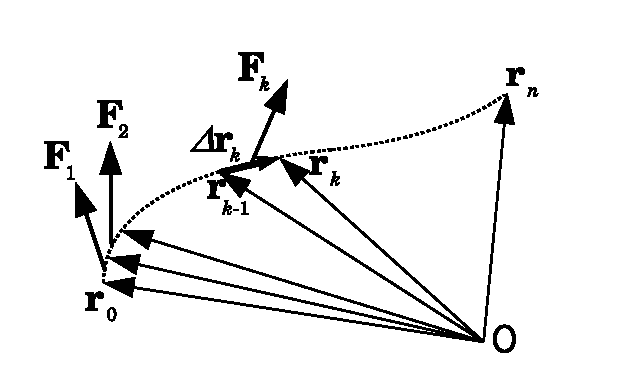
\includegraphics[width=7cm]{work_3D.eps}
    \caption{質点の動く経路を細かく分割する。}\label{fig:work_3D}
\end{figure}
この2点の間で力がなす仕事$\Delta W_k$は, 
\eref{eq:work_Fdotdr}より
$\Delta W_k\fallingdotseq{\bf F}_k\bullet\Delta {\bf r}_k$
となる。これを全区間について合計すれば, ${\bf r}_0$から${\bf r}_n$までの
移動でなされる仕事$W$になる:
\begin{eqnarray} 
W\fallingdotseq\sum_{k=1}^n \Delta W_k\fallingdotseq\sum_{k=1}^n {\bf F}_k\bullet\Delta {\bf r}_k
\end{eqnarray}
これは\eref{eq:one_step_before_work2}を3次元に拡張した式でもある。 
ここで刻みをどんどん小さくしていけば, 
\begin{eqnarray}
W=\lim_{\substack{n\rightarrow \infty\\\Delta {\bf r}_k\rightarrow 0}}\quad\sum_{k=1}^n{\bf F}_k\bullet\Delta {\bf r}_k
\end{eqnarray}
となる。これは積分の定義より($\Sigma$は$\int$になり, $\Delta$は$d$になる!), 
\begin{eqnarray} 
W=\int_{{\bf r}_0}^{{\bf r}} {\bf F}\bullet d{\bf r}
\end{eqnarray} 
となる(${\bf r}_n$を改めて${\bf r}$とおいた)。

\begin{faq}{\small\textgt{何ですかこの積分!? 
普通の積分は, $\int$なんちゃら$dx$とか$\int$なんちゃら$dt$みたいに, $d$が
つくのは$x$や$t$などです。でも, これは$d{\bf r}$って, ベクトルに
$d$がついてます。しかも内積!?} ... 
初めて見たらちょっとびっくりしますよね。でも, これはそんなに不思議なことではありません。
積分の定義を思い出して下さい。「関数と微小量の掛け算」が, ここでは
力(位置の関数で, ベクトル)と変位(位置の変化を表す微小量で, ベクトル)
の内積(掛け算をベクトルに拡張したもの)になっているだけです。}\end{faq}\mv

この式は\eref{eq:work2}を3次元に拡張した式だ。この積分は, 始点${\bf r}_0$と
終点${\bf r}$のみならず, 移動の経路にも依存するから, その経路を$\Gamma$と名づければ, 
以下のように言える: 経路$\Gamma$を移動する質点にかかる力${\bf F}$のなす仕事を, 
次式で定義する:
\begin{eqnarray}
W=\int_{\Gamma} {\bf F}\bullet d{\bf r}\label{eq:def_work_3D}
\end{eqnarray} 
ここで, ${\bf r}$は位置ベクトル。この式は, 最も一般的な仕事の定義式である。

ここで出てきた積分は, 君にとって目新しいものだろう。ここでは被積分関数も積分変数も
ベクトルであり, 「関数と微小量の掛け算」がここではベクトルの内積であり, 
しかも積分区間が「経路$\Gamma$」であるのだ。このように, ある経路に
沿って, ベクトルと微小ベクトルの内積を足し合わせるような積分を, 
\underline{線積分}\index{せんせきぶん@線積分}という。3次元では, 仕事は
線積分で定義されるのだ。\mv

\begin{q}\label{q:work_3D}
仕事を3次元空間で定義せよ。
\end{q}
\hv


\section{3次元空間におけるポテンシャルエネルギー}

次に, 「ポテンシャルエネルギー」の定義を3次元空間に拡張しよう。といっても, 
仕事の定義を上述のように改めること以外は, ポテンシャルエネルギーの定義は
1次元のときと同じだ。\eref{eq:potential}, つまり, 
\eref{eq:potential2}, \eref{eq:potential3}の位置$x$を
位置ベクトル${\bf r}$に置き換えたものが, 3次元空間における
ポテンシャルエネルギーだ。すなわち, ポテンシャルエネルギーを$U({\bf r})$とすると, 
\begin{eqnarray}
\text{定義1': }U({\bf r}):=-W({\bf r})\label{eq:3Dpotential}
\end{eqnarray}
ここで$W({\bf r})$は, 物体を基準点から点${\bf r}$まで運ぶときに, 
物体にかかっている保存力がなす仕事。
\begin{eqnarray}
\text{定義2': }U({\bf r}):=W'({\bf r})\label{eq:3Dpotential2}
\end{eqnarray}
ここで$W'({\bf r})$は, 物体を基準点から点${\bf r}$まで運ぶときに, 
かかっている保存力に逆らって誰かがなす仕事。
\begin{eqnarray}
\text{定義3': }U({\bf r}):=W''({\bf r})\label{eq:2Dpotential3}
\end{eqnarray}
ここで$W''({\bf r})$は, 物体を点${\bf r}$から基準点まで運ぶときに, 物体に
かかっている保存力がなす仕事。\\

無論, これらの3つの定義は互いに同値だ。力が保存力でなければ
ならない, ということに注意しよう。\mv

%
\begin{q}\label{q:3D_work_conservative}
物体が保存力${\bf F}$を受けて, ある点${\bf r}_0$から別の点${\bf r}_1$まで
移動するとき, ${\bf F}$がなす仕事$W_{01}$は, 
\begin{eqnarray}
W_{01}=U({\bf r}_0)-U({\bf r}_1)\label{3D_work_conservative}
\end{eqnarray}
であることを示せ。ここで$U$はポテンシャルエネルギーである。
\end{q}

%
\begin{q}\label{q:work_conservative_loop}
保存力が, 3次元空間の任意の閉曲線(始点と終点が一致する曲線)に沿ってなす仕事は, 必ず0になることを示せ。
\end{q}
\hv



\section{3次元空間における力学的エネルギー保存則}

役者は揃った。ではいよいよ, 力学的エネルギー保存則が3次元でも成り立つことを確認していこう。
1次元で力学的エネルギー保存則を導いたとき, \eref{eq:WandT00}から\eref{eq:WandT00s}に
かけて, 運動方程式を位置で積分した。3次元でも同じ事をやるのだ。まず, 運動方程式:
\begin{eqnarray}
{\bf F}=m\frac{d{\bf v}}{dt}\label{eq:3D_cons_F_ma}
\end{eqnarray}
を考える。${\bf F}$, ${\bf v}$, $m$, $t$はそれぞれ質点に働く力, 質点の速度, 質点の質量, 
そして時刻である。質点の位置ベクトルを${\bf r}(t)$とする。時刻$t$と, そこから
微小時間$dt$だけ経過した$t+dt$で, 質点は少し違う位置にいる(移動している)。その差, 
つまり変位を$d{\bf r}$と書こう。つまり, 
\begin{eqnarray}
d{\bf r}={\bf r}(t+dt)-{\bf r}(t)
\end{eqnarray}
である。この両辺を$dt$で割ったもの(つまり位置を時刻で微分したもの)
が速度${\bf v}$だ。つまり, ${\bf v}=d{\bf r}/dt$だ。従って, 次式が成り立つ:
\begin{eqnarray}
d{\bf r}={\bf v}dt\label{eq:3D_cons_dr_vdt}
\end{eqnarray}
\eref{eq:3D_cons_F_ma}に\eref{eq:3D_cons_dr_vdt}を辺々, 内積すると次式を得る:
\begin{eqnarray}
{\bf F}\bullet d{\bf r}=m\frac{d{\bf v}}{dt}\bullet {\bf v}dt\label{eq:3D_WandT000}
\end{eqnarray}
これはちょうど, \eref{eq:WandT000}を3次元に拡張した式だ。

ここで, 時刻$t_0$から$t_1$までの運動を考える。
${\bf r}_0={\bf r}(t_0)$, 
${\bf r}_1={\bf r}(t_1)$, 
${\bf v}_0={\bf v}(t_0)$, 
${\bf v}_1={\bf v}(t_1)$
とし, ${\bf r}_0$から${\bf r}_1$までの質点の運動の軌跡を$\Gamma$とする。
$\Gamma$をたくさんの短い区間に分割し, それぞれの区間で\eref{eq:3D_WandT000}
を考えて足し合わせる。つまり, 時刻$t_0$から$t_1$までの間で, 
\eref{eq:3D_WandT000}を積分すると, 
\begin{eqnarray}
\int_{\Gamma}{\bf F}\bullet d{\bf r}=\int_{t_0}^{t_1}m\frac{d{\bf v}}{dt}\bullet {\bf v}dt\label{eq:3D_WandT00s}
\end{eqnarray}
となる。左辺は\eref{eq:def_work_3D}の右辺
と同じ形になっている。つまり, 質点に働く力がなす仕事$W_{01}$である。

ここで, ${\bf v}=(v_x, v_y, v_z)$とすれば, 
\begin{eqnarray}
\frac{d{\bf v}}{dt}=\Bigl(\frac{dv_x}{dt}, \frac{dv_y}{dt}, \frac{dv_z}{dt}\Bigr)
\end{eqnarray}
である。これらを使って\eref{eq:3D_WandT00s}の右辺を成分で書くと, 次のようになる:
\begin{eqnarray}
&&\int_{t_0}^{t_1}m\Bigl(\frac{dv_x}{dt}, \frac{dv_y}{dt}, \frac{dv_z}{dt}\Bigr)\bullet(v_x, v_y, v_z)dt\\
&&=\int_{t_0}^{t_1}m\Bigl(v_x\frac{dv_x}{dt}+v_y\frac{dv_y}{dt}+v_z\frac{dv_z}{dt}\Bigr)dt\\
&&=\int_{t_0}^{t_1}mv_x\frac{dv_x}{dt}dt+\int_{t_0}^{t_1}mv_y\frac{dv_y}{dt}dt+\int_{t_0}^{t_1}mv_z\frac{dv_z}{dt}dt\nonumber\\
&&=\int_{v_x(t_0)}^{v_x(t_1)}mv_x\,dv_x+\int_{v_y(t_0)}^{v_y(t_1)}mv_y\,dv_y+\int_{v_z(t_0)}^{v_z(t_1)}mv_z\,dv_z\nonumber\\
&&=\Bigl[\frac{1}{2}m v_x^2\Bigr]_{v_x(t_0)}^{v_x(t_1)}+\Bigl[\frac{1}{2}m v_y^2\Bigr]_{v_y(t_0)}^{v_y(t_1)}+\Bigl[\frac{1}{2}m v_z^2\Bigr]_{v_z(t_0)}^{v_z(t_1)}\nonumber\\
&&=\frac{1}{2}m\bigl(v_x^2(t_1)+v_y^2(t_1)+v_z^2(t_1)\bigr)\nonumber\\
&&\,\,\,\,-\frac{1}{2}m\bigl(v_x^2(t_0)+v_y^2(t_0)+v_z^2(t_0)\bigr)\\
&&=\frac{1}{2}m{\bf v}_1^2-\frac{1}{2}m{\bf v}_0^2
\end{eqnarray}
となる。従って, \eref{eq:3D_WandT00s}は次式のようになる:
\begin{eqnarray}
W_{01}=\frac{1}{2}m{\bf v}_1^2-\frac{1}{2}m{\bf v}_0^2\label{eq:3DWandT0}
\end{eqnarray}
ここで\eref{eq:kineticEnergy3D0}を使うと, \eref{eq:3DWandT0}は
\begin{eqnarray}
W_{01}=T({\bf v}_1)-T({\bf v}_0)\label{eq:3D_WandT2}
\end{eqnarray}
となる。ここで, $T({\bf v})$は質点の運動エネルギーである。

\eref{eq:3D_WandT2}は, 1次元で導いた\eref{eq:WandT2}と同じ形の式だ。
つまり, 3次元の運動でも, 力がなした仕事は運動エネルギーの変化に等しい, 
ということが成り立つ。

ところで, \underline{力が保存力の場合は}, \eref{eq:3D_WandT2}の
左辺を\eref{3D_work_conservative}で書き換えると, 
\begin{eqnarray}
U({\bf r}_0)-U({\bf r}_1)=T({\bf v}_1)-T({\bf v}_0)\label{3D_work_conservative0}
\end{eqnarray}
となる。あるいは, 
\begin{eqnarray}
T({\bf v}_0)+U({\bf r}_0)=T({\bf v}_1)+U({\bf r}_1)\label{3D_work_conservative1}
\end{eqnarray}
となる。すなわち, 運動の最初(時刻$t_0$)と運動の最後(時刻$t_1$)で, 
「運動エネルギーとポテンシャルエネルギーの和」は等しいのだ。1次元のときと同様に, 
「運動エネルギーとポテンシャルエネルギーの和」のことを, 「力学的エネルギー」と
呼ぼう(定義)。すなわち, \eref{3D_work_conservative1}によって, 3次元における
力学的エネルギー保存則が確かめられた!\\

\begin{q}\label{q:consmom3D} 運動方程式から\eref{3D_work_conservative1}を導出せよ
(上の議論を整理・再現すればよい)。\end{q}


\begin{figure}[h]
    \centering
    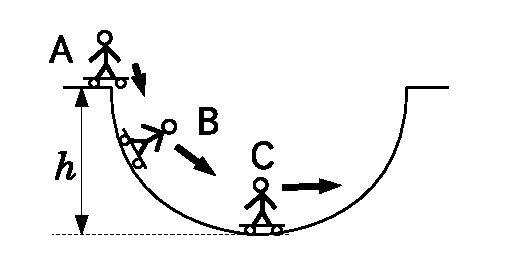
\includegraphics[width=7cm]{half_pipe.eps}
    \caption{スケートボードのハーフパイプ}\label{fig:half_pipe}
\end{figure}
\begin{q}\label{q:half_pipe}
スケートボードで, ハーフパイプを降りる人(スケートボードとあわせて質量$m$)の運動を考えよう(図\ref{fig:half_pipe})。
ハーフパイプの縁Aにいるときは速さ0である。そこから静かにハーフパイプの側面を降りはじめ, 
重力にまかせて加速しながら降りていき(点B), ハーフパイプの底(点C)に至る。点Cに至ったときは, 速さ$v$で水平方向に
動いている。ハーフパイプの底と縁の高度差は$h$であるとする。ただし摩擦や空気抵抗や車輪の回転に伴うエネルギーなどは無視する。
\begin{enumerate}
\item 重力加速度を$g$とする。次式を示せ:
\begin{eqnarray}\frac{1}{2}mv^2=mgh\end{eqnarray}
\item $h=5.0$~mのとき, $v$を求めよ。
\item ハーフパイプの断面が半円だとすると, 点Cでその人が受ける垂直抗力の大きさは重力の何倍か?
\end{enumerate}\end{q}

\section{振り子の運動}\index{ふりこ@振り子}

振り子の運動を考えてみよう。天井に固定された点Pから長さ$l$の糸が垂れており, 
その先に質量$m$の質点がついている(図\ref{fig:pendulum})。
質点が最も下に来たとき(糸が鉛直になったとき)の位置をOとする。糸をぴんと
張ったまま質点を少し持ち上げたときの
位置をQとする。Qから静かに質点を手放すと, 質点はP, O, Qを含む鉛直平面内で振動運動をする。

時刻$t$で質点は点X($t$)にあるとし, 角OPXをラジアンであらわしたものを$\theta$としよう。
当然, $\theta$は時間の関数だ。
以下, 糸の質量は0とする。空気抵抗は無視する。\mv
\begin{figure}[h]
    \centering
    \includegraphics[width=7cm]{pendulum.eps}
    \caption{振り子}\label{fig:pendulum}
\end{figure}

\begin{q}\label{q:furiko_energy} この質点の運動について, \\
(1) 時刻$t$における質点の速度を${\bf v}(t)$とすると, 
\begin{eqnarray} 
|{\bf v}(t)|=\Bigl|l\frac{d\theta}{dt}\Bigr|
\end{eqnarray} 
であることを示せ。{\small ヒント:$t$から$t+dt$の間に$X$が移動するのは, 扇形の
弧の部分である。その弧の長さ(つまり移動距離)は, 
「半径」かける「角度の変化」であり, 「角度の変化」
は$\theta(t+dt)-\theta(t)$である。また, 速度の絶対値(つまり速さ)とは, 
$t$から$t+dt$の間に$X$が移動した距離を時間間隔$dt$で割ったものだ。}\\
(2) 時刻$t$における質点の運動エネルギー$T$とポテンシャルエネルギー$U$は, それぞれ
次のようになることを示せ:
\begin{eqnarray} 
T&=&\frac{1}{2}m l^2\Bigl(\frac{d\theta}{dt}\Bigr)^2\\
U&=&mgl(1-\cos \theta)
\end{eqnarray} 
ただし, 質点が点Oにあるとき$U=0$と定める。\\
(3) 働く力は重力と張力だけだが, 重力は保存力であり, 張力は仕事をしない
(移動方向と力の方向が直交しているので)。従って力学的エネルギー保存則が成り立つ。
すなわち, $T+U$は時刻$t$によらず一定である。従って, 
$T+U$を$t$で微分すると, 0にならねばならない。このことから, 次式を導け:
\begin{eqnarray} 
ml^2\frac{d\theta}{dt}\frac{d^2\theta}{dt^2}+mgl\sin\theta\frac{d\theta}{dt}=0
\end{eqnarray} 
(4) その結果, 次式(振り子の運動をあらわす微分方程式)を得ることを示せ:
\begin{eqnarray} 
\frac{d^2\theta}{dt^2}=-\frac{g}{l}\sin\theta\label{eq:furiko_equation}
\end{eqnarray} 
(5) $\theta$が0に近い場合, 振り子の運動方程式は, 近似的に次のようになることを示せ:
\begin{eqnarray} 
\frac{d^2\theta}{dt^2}=-\frac{g}{l}\theta\label{eq:furiko_energy5}
\end{eqnarray} 
この近似式が成り立つとして, 以下の小問に答えよ:\\
(6) $\omega=\sqrt{g/l}$とすると\eref{eq:furiko_energy5}は次式になることを示せ
(これは関数$\theta(t)$に関する微分方程式):
\begin{eqnarray} 
\frac{d^2\theta}{dt^2}=-\omega^2\theta\label{eq:furiko_energy6}
\end{eqnarray} 
(7) $\theta(t)=\theta_0 \cos\omega t$は上の微分方程式の解であることを示せ。ただし$\theta_0$は定数とする。\\
(8) 振り子の周期$\tau$を, $g$と$l$であらわせ\footnote{普通は周期は$T$で表す慣習が多いが, ここでは$T$は運動エネルギーの記号に使っているので, 周期は$\tau$(ギリシア文字のタウ)を使う。}。\\
(9) $l=1.0$~mのとき, 振り子の振動の角速度と周期は?\\
(10) $l$を何倍にすれば振り子の周期は半分になるか?
\end{q}


\begin{q}\label{q:furiko_period}
前問で見たように, \underline{振幅が十分に小さいとき} \underline{に限れば}
(すなわち$\theta$が0に近ければ), 振り子の周期は糸の長さ$l$と重力加速度$g$
だけで決まってしまい, 質点の質量$m$や, 振れ幅$\theta_0$などには依らない。これは, 振り子の
重要な性質である(これを「振り子の等時性という」\index{とうじせい@等時性})。
\begin{enumerate}
\item これを利用して, 重力加速度$g$を測定する。つまり, 長さ$l$の糸の先に適当な重り
をつけて振動させ, その周期$\tau$を測ったとする。では, $l$と$\tau$から$g$を求める式は? 
\item 月面では, 地球上に比べて振り子の周期は何倍になるか? 
\end{enumerate}
\end{q}

\begin{q} 2つの互いに同仕様の振り子時計がある。これらの時刻を互いに合わせた後, 
東京(重力加速度9.798~m~s$^{-2}$)と札幌(重力加速度9.805~m~s$^{-2}$)
のそれぞれに置いた。1日たつと, 札幌の時計は東京の時計より何秒, 進んでいる
(もしくは遅れている)か?\end{q}
\mv

\begin{faq}{\small\textgt{振り子といえばフーコーですね。振り子で地球の自転を証明したんですよね} ... 
そうです。自転によって生じる「コリオリ力」という見かけの力を実証しました。}\end{faq}\mv
\hv

\section{ポテンシャルエネルギーと力の関係}

{\small (本節は後の話に関係しないので読み飛ばしてもよい。
秋学期に電磁気学を学ぶ時に復習すると役立つだろう。)\\}

さて, 力学的エネルギー保存則の話から少し外れるが, ここで力とポテンシャルエネルギーの関係をもう少し深くみておこう。
いま, 符号を無視しておおまかに言えば, 力の(線)積分がポテンシャルエネルギーを与えるわけだから, 積分と微分は
互いに逆の操作であることを考えれば, ポテンシャルエネルギーの微分が力を与えるのではないだろうか? 
実は, この発想は正しい。以下にそれを説明しよう:

いま, ある質点に働く力が保存力であり, しかも場所だけによって一意的に定まり, 時刻や速度など
には陽に依存しない\footnote{この「陽に」(explicit)という言葉は科学ではよく使う。「あからさまに」
とか「直接的に」という意味。今の場合は, 時間と共に場所が変われば力も変わるかもしれないが, 
それは場所が変わったからであり, 時間の変化が直接的に力を変えたわけではない, ということ。}
としよう。

とりあえず, 簡単のため, 物体の移動は直線上($x軸$の上)に制限され, 働く力もその直線に沿った方向に
限定されるとしよう。物体が位置$x_0$から$x_1$まで動くときに, 力$F$がなす仕事$W_{01}$は, 
\eref{eq:W01U1U0}より, 
\begin{eqnarray}
W_{01}=-U(x_1)+U(x_0)
\end{eqnarray}
である($U$はポテンシャルエネルギー)。ここで, $x_0$を$x$とし, $x_1$を$x$から非常に近い位置$x+dx$とすると($dx$は0に近い量), 
\begin{eqnarray}
W_{01}=-U(x+dx)+U(x)\label{eq:W01UxdxUx}
\end{eqnarray}
となる。ところで, 仕事の定義から, $W_{01}$は
$W_{01}=F\,dx$である。これらから, 
$F\,dx=-U(x+dx)+U(x)$
となる。両辺を$dx$で割って, 
\begin{eqnarray}
F=-\frac{U(x+dx)-U(x)}{dx}
\end{eqnarray}
ここで$dx$が十分に0に近いことを思い出せば, 
\begin{itembox}{ポテンシャルエネルギーと力の関係(1次元)}
\begin{eqnarray}
F=-\frac{dU}{dx}
\end{eqnarray}
\end{itembox}
である。つまり, 力は, ポテンシャルエネルギーを微分してマイナスをつけたものに等しい。\mv

この話は3次元空間に拡張できる。物体が力${\bf F}$を受けながら位置${\bf r}$から, 
わずかだけ離れた位置${\bf r}+d{\bf r}$に移動することを考える。
\begin{eqnarray}
d{\bf r}=(dx,\, dy,\, dz)
\end{eqnarray}
は十分に小さいベクトルである。
すると, 力がなす仕事$W$は, \eref{eq:W01UxdxUx}と同じように考えれば, 
\begin{eqnarray}
W=-U({\bf r}+d{\bf r})+U({\bf r})\label{eq:dW3D}
\end{eqnarray}
である($U$はポテンシャルエネルギー)。ここで全微分\footnote{数学の教科書を参照。}を使うと, 
$U({\bf r}+d{\bf r})=U(x+dx, y+dy, z+dz)$
\begin{eqnarray}
&=&U(x, y, z)+\frac{\partial U}{\partial x}dx+\frac{\partial U}{\partial y}dy+\frac{\partial U}{\partial z}dz\nonumber\\
&=&U({\bf r})+\frac{\partial U}{\partial x}dx+\frac{\partial U}{\partial y}dy+\frac{\partial U}{\partial z}dz\,\,\,\,\,\,\,\,\,\,\,\,\,\,\,\,\,\,\,\,\,\,\,
\end{eqnarray}
である。これを\eref{eq:dW3D}に代入すると次式になる:
\begin{eqnarray}
W&=&-U({\bf r})-\frac{\partial U}{\partial x}dx-\frac{\partial U}{\partial y}dy-\frac{\partial U}{\partial z}dz+U({\bf r})\nonumber\\
 &=&-\frac{\partial U}{\partial x}dx-\frac{\partial U}{\partial y}dy-\frac{\partial U}{\partial z}dz\nonumber\\
 &=&-\Bigl(\frac{\partial U}{\partial x}, \frac{\partial U}{\partial y}, \frac{\partial U}{\partial z}\Bigr)\bullet(dx, dy, dz)\nonumber\\
 &=&-\Bigl(\frac{\partial U}{\partial x}, \frac{\partial U}{\partial y}, \frac{\partial U}{\partial z}\Bigr)\bullet d{\bf r}
\end{eqnarray}
一方, 仕事の定義から$W$は$W={\bf F}\bullet d{\bf r}$なので, 
\begin{eqnarray} 
{\bf F}\bullet d{\bf r}=-\Bigl(\frac{\partial U}{\partial x}, \frac{\partial U}{\partial y}, \frac{\partial U}{\partial z}\Bigr)\bullet d{\bf r}\label{eq:Fdr_gradUdr}
\end{eqnarray} 
である。$dx, dy, dz$は0に近い任意の量なので, 上の式が成り立つには, 
\begin{itembox}{ポテンシャルエネルギーと力の関係(3次元)}
\begin{eqnarray} 
{\bf F}=-\Bigl(\frac{\partial U}{\partial x}, \frac{\partial U}{\partial y}, \frac{\partial U}{\partial z}\Bigr)\label{eq:F_gradU}
\end{eqnarray} 
\end{itembox}
でなければならない\footnote{
${\bf F}=(F_x, F_y, F_z)$とする。\eref{eq:Fdr_gradUdr}で$dx\ne0$として$dy=dz=0$とすると, 
\begin{eqnarray*}F_x\,dx=-\frac{\partial U}{\partial x}\,dx,\,\,\,\,\,\,\,\text{したがって, }\,\,\,F_x=-\frac{\partial U}{\partial x}\end{eqnarray*}
を得る。$dy\ne0$で$dx=dz=0$の場合や, $dz\ne0$で$dx=dy=0$の場合も同様に考えれば, 
\begin{eqnarray*}F_y=-\frac{\partial U}{\partial y},\,\,\,\,F_z=-\frac{\partial U}{\partial z}\end{eqnarray*}
を得る。したがって\eref{eq:F_gradU}が成り立つ。}。ここで, "grad"という記号を, 
\begin{eqnarray}
\grad U=\Bigl(\frac{\partial U}{\partial x}, \frac{\partial U}{\partial y}, \frac{\partial U}{\partial z}\Bigr)
\end{eqnarray}
と定義する\footnote{このgradとは, "gradient"の略であり, 日本語では「勾配」と言う。
その意味は, いずれ基礎数学や秋学期の物理学で学ぶだろう。}。この記号を使うと, 
\eref{eq:F_gradU}は次式のように書ける:
\begin{eqnarray} 
{\bf F}=-\grad U\label{eq:F_gradU2}
\end{eqnarray} 
\mv

\begin{exq} アインシュタインの相対性理論によると, 重力によるポテンシャル
エネルギーが高い位置ほど時間は速く進む(とても不思議!)。すなわち, ある
2つの位置A, Bがあって, 重力によるポテンシャルエネルギーが, 位置Bでは
位置Aよりも$m\phi$だけ高いとし($m$は質点の質量), 位置Aに置かれた時計が
時間$T$だけ進む場合, 位置Bに置かれた時計は, 以下のぶんだけ進む。
\begin{eqnarray}
T\Bigl(1+\frac{\phi}{c^2}\Bigr)
\end{eqnarray}
ここで, $c=299792458$~m/sは光の速さである。
以後, 地球の半径を$R=6400$~kmとする。\\
(1) GPS衛星は地表から約20,000~kmの高さを飛んでいる。地上の時計が
1秒進む間に, GPS衛星に搭載された時計は, 1秒よりどれだけ多くの時間を進むか? 
(他の要因のために, 実際に起きるのは, ここで計算される値よりも, 若干小さい値である)\\
(2) 高精度の時計が2つあれば, これらの時計が示す時刻の差から, これらの時計の
置かれた高さの差がわかる。つまり, 時計を高度計として使うことができるだろう。
ところで, 東大の香取秀俊博士が開発した「光格子時計」は, 300億年に1秒しか狂わない
という, 世界的にもブッチギリな高精度を持つ。この時計を高度計として使う場合, 
地表付近(海面から高さ±数kmの範囲)では, どのくらいの誤差で高度を計測できるか?
\end{exq}

なお, この「高度計」が素晴らしいのは, GPSのような衛星からの電波が入ってこない水中や
地下, 屋内などでも原理的には利用可能ということである。\\

\section{解答}
% 仕事を3次元空間で定義せよ。
%\noindent{\textbf{答}}\ref{q:work_3D} 質点を経路$\Gamma$に沿って移動するとき, 
%各位置で質点にかかる力を${\bf F}$とすると, その経路に沿って${\bf F}$が質点に
%対してなした仕事$W$は, 
%\begin{eqnarray*} 
%W=\int_{\Gamma} {\bf F}\bullet d{\bf r}
%\end{eqnarray*}
%である。\mv
\noindent{\textbf{答}}\ref{q:work_3D} 略。\mv

%
\begin{figure}[h]
    \centering
    \includegraphics[width=5.0cm]{cons_force_3D.eps}
    \caption{問\ref{q:3D_work_conservative}の仕事の経路。}\label{fig:cons_force_3D}
\end{figure}
\noindent{\textbf{答}}\ref{q:3D_work_conservative}
物体を基準点から点${\bf r}_0$まで運ぶときに保存力${\bf F}$
がなす仕事を$W({\bf r}_0)$とすると, 定義から, 
\begin{eqnarray}
U({\bf r}_0)=-W({\bf r}_0)\label{q:3D_work_conservative_ans1}
\end{eqnarray}
である。同様に, 物体を基準点から点${\bf r}_1$まで運ぶときに保存力${\bf F}$
がなす仕事を$W({\bf r}_1)$とすると, 
\begin{eqnarray}
U({\bf r}_1)=-W({\bf r}_1)\label{q:3D_work_conservative_ans2}
\end{eqnarray}
である。ここで, 基準点から点${\bf r}_1$へ物体を運ぶときの経路を, 点${\bf r}_0$を
経由するようにとれば(図\ref{fig:cons_force_3D}), 保存力ゆえに仕事は経路によらず一定なので, 
$W({\bf r}_1)=W({\bf r}_0)+W_{01}$
となる。ここで$W_{01}$は物体を点${\bf r}_0$から点${\bf r}_1$に運ぶときの仕事。
この式の$W({\bf r}_0), W({\bf r}_1)$を, 
\eref{q:3D_work_conservative_ans1}, \eref{q:3D_work_conservative_ans2}を
使って置き換えると, 
$-U({\bf r}_1)=-U({\bf r}_0)+W_{01}$
となる。従って, 
$U({\bf r}_0)-U({\bf r}_1)=W_{01}$。
\mv

% 保存力が, 3次元空間の任意の閉曲線に沿ってなす仕事は, 必ず0に
\noindent{\textbf{答}}\ref{q:work_conservative_loop}
閉曲線$\Gamma$に沿う移動によってなす仕事を$W$とする。
移動の開始点を${\bf r}_0$とすると, 移動の終了点も${\bf r}_0$である。保存力だから, 
\eref{3D_work_conservative}で, ${\bf r}_1={\bf r}_0$, $W_{01}=W$として, 
$W=U({\bf r}_0)-U({\bf r}_0)$となる。右辺は0だから, 結局, $W=0$となる。\mv


\noindent{\textbf{答}}\ref{q:half_pipe} 
(1) 点Cをポテンシャルエネルギーの基準点とする。点Aでは, 運動エネルギーは0, 
ポテンシャルエネルギーは$mgh$である。従って力学的エネルギーは$mgh$となる。
点Cでは, 運動エネルギーは$mv^2/2$, ポテンシャルエネルギーは0である。従って力学的エネルギーは$mv^2/2$となる。
働く力は重力と垂直抗力だけだが, 重力は保存力であり, 垂直抗力は仕事をしない(移動方向と力の方向が直交しているので)。
従って力学的エネルギー保存則が成り立つ。すなわち, 点Aと点Cで力学的エネルギーは等しいことから, 与式を得る。\\
(2) 前小問より,
\begin{eqnarray*}
v=\sqrt{2gh}=\sqrt{2\times9.8\text{ m s}^{-2}\times5\text{ m}}=9.9\text{ m s}^{-1}
\end{eqnarray*}
(3) 半円形ハーフパイプの高さが$h$なのだから, この円の半径は$h$である。
\eref{eq:mvsqovr}より, C点では人は円の中心に向かって(つまり上向きに), 
$mv^2/h$という合力を受けるはず。
一方, 垂直抗力を$N$とする。人には下向きに$mg$という重力も働くから, 
上向きの力は, 垂直抗力と重力の合力であり, その大きさは$N-mg$である。従って, 
$N-mg=mv^2/h$である。従って, 
\begin{eqnarray}N=\frac{mv^2}{h}+mg\end{eqnarray}
である。小問(1)より$mv^2=2mgh$だから, 
\begin{eqnarray}N=2mg+mg=3mg\end{eqnarray}
となる。よって垂直抗力は, 半径$h$によらず, 重力の3倍。だからハーフパイプ走者は
重力の3倍の力に耐える頑丈な肉体を持っていなければならない。
\mv

% 天井に固定された点Pから長さ$l$の糸が垂れており, その先に
\noindent{\textbf{答}}\ref{q:furiko_energy} 
(1) $t$から$t+dt$の間に$X$が移動する距離は, \\
$l|\theta(t+dt)-\theta(t)|$である。微分の定義から, 
これは$l|\theta'dt|$に等しい。これを$dt$で割ったものが速度の大きさになる。したがって与式が成り立つ。
(2) 略($T=mv^2/2$の$v$に前小問の結果を代入すると, 運動エネルギー$T$の与式を得る。また, Oに比べてX
は$l(1-\cos\theta)$だけ高い位置にある。従って, 重力によるポテンシャルエネルギー$U$の与式を得る。)
(3), (4) 略。
(5) 略。($\sin \theta \fallingdotseq \theta$とすればよい)
(6) 略。
(7) 略(\eref{eq:furiko_energy6}の左辺と右辺に代入して, それらが等しくなることを示せばよい)。
(8) $\tau=2\pi/\omega$より(\eref{eq:vib_period}) 参照), 
\begin{eqnarray}\tau=2\pi\sqrt{l/g}\label{eq:furiko_energy_ans5}\end{eqnarray}
(9) 角速度は, $\omega=\sqrt{g/l}=\sqrt{9.8\text{ m s}^{-2}/(1.0\text{ m})}=3.1\text{ s}^{-1}$。周期は(計算略), $\tau=2\pi/\omega=2.0$ s。\\
(10) \eref{eq:furiko_energy_ans5}より, $\tau$は$\sqrt{l}$に比例するから, $\tau$を半分にするには, $\sqrt{l}$を半分にすればよい。従って$l$を1/4倍にすればよい。
\mv

% 前問で見たように, 振幅が十分に小さければ, 振り子の周期は
\noindent{\textbf{答}}\ref{q:furiko_period}
(1) \eref{eq:furiko_energy_ans5}を変形して$g=$の式にすると, 
$g=4\pi^2l/\tau^2$。
(2) 月面では重力加速度が地表の1/6倍になる。\eref{eq:furiko_energy_ans5}より, 
$\tau$は$1/\sqrt{g}$に比例するから, $g$が1/6倍になると$\tau$は$\sqrt{6}=2.4$倍(ゆっくり振動)。
\mv


\begin{faq}{\small\textgt{ポテンシャルエネルギーは, 力学的エネルギー保存則
を見やすくするために定義されたもの, と考えてよいのですか?} ... 
それだけではありません。まず, 力はベクトルだけどポテンシャルエネルギーはスカラーなので, 
力を直接考えるよりも, 数学的に取扱いがシンプルで楽になります。また, 量子力学では力よりも
ポテンシャルエネルギーの方が直接的に重要な働きをします。}\end{faq}

\begin{faq}{\small\textgt{力学的エネルギー保存則と
エネルギー保存則は違うんですね?} ... 違うというより, 
前者は後者の一種(特別なケース)ですね。}\end{faq}

\begin{faq}{\small\textgt{「保存力は径路に依存しない」というフレーズが頭にしっくりこない。} ... 
ちょっと省略しすぎですね。「保存力がなす仕事は, 径路によらず, 始点と終点だけで
決まる」というのが正しい表現です。例え話でいうと, 山を登るのに, きつい勾配の坂を
まっすぐ登るのと, ジグザグになった緩やかな道を登るのとでは, 全体の仕事(力かける距離)
は同じということです。きつい道では大きな力が(移動方向に)かかるけど, そのぶん
短くてすみます。}\end{faq}

\section*{コラム: ベクトルは太字, スカラーは細字なのはなぜか?}

{\small 「ベクトルは太字で書く」が, ちゃんとできない人が多い。そもそもなぜベクトルは特別な
書き方(太字で書く)をするのだろう?それは, スカラーとベクトルは, 本質的に違う量
であり, 計算ルールも異なるからだ。

例えば「スカラーでの割り算」は(0で割る以外は)許されるが, 「ベクトルでの割り算」は
許されない。スカラー同士やベクトル同士は足せるが, スカラーとベクトルは足せない。
スカラーとベクトルの大小関係は比べられないし, スカラーとベクトルが等号で結ばれる
こともない。それらの「ルール破り」を防ぐための「要注意記号」として, ベクトルを太字や
上付き矢印で書くのだ。

ベクトルは太字という慣習を守らない人は, そもそも何がベクトルで何がスカラーかを
わかっていない可能性がある。それはかなりヤバイ。ベクトルを太字で書かないと減点されるのは, 
「わかってる風を装っているだけで, 実はわかっていない」のではないかと思われているのだ。
逆に言えば, 「自分はどれがベクトルでどれがスカラーなのかちゃんとわかってるぜ!」
ということをアピールするために, ベクトルを太字で書くのだ。

ところが, ひとつの直線上に限定された現象(直線運動)では, ベクトルとスカラーを
区別する必要はないので, 本来ベクトルである量もスカラーとして扱い, 
細字で書く。このような場合も, 力や速度や加速度には向きがあるが, 
それは符号(正か負か)で表現できるので, スカラーで十分であり, 
わざわざベクトルとして扱う必要は無い。ベクトルとして扱っても, 
数値で表現するときは, ひとつの数値(成分)しかない。

数学や物理では, 「区別すべきものは区別せねばならないが, 区別する必要のない
ものは, 理由もないのに区別したりしてはいけない」という
慣習がある(例外もあるが)。これに照らせば, 直線上に限定されることが最初から
わかっている運動では$F=ma$のように書いてよいし, むしろそう書かねばならない
($F, m, a$は力, 質量, 加速度)。この場合は$F$や$a$はスカラーと
同様に扱うことができ, $m=F/a$と書けるからでもある($a\neq 0$の場合)。\\}


\section*{コラム: 問題を解くコツ}

{\small 物理学の問題を解くには, いくつかのコツがある。\\

1. 値の代入は最後にやる!

既に述べたが, 答を数値で求める問題も, できるだけぎりぎりまで, 数値ではなく文字の式変形で攻めよう。そして, 求めたい量を既知の量で表す式が求まった段階で, 既知の量の数値を代入して一気にまとめて数値計算をするのである。最初や途中から数値を代入してしまうと, 式変形と数値計算が混在してしまい, ミスを起こしやすく, また, ミスの発見がやりにくくなる。一方, 最後にまとめて計算すれば, 約分の組み合わせがたくさんできるので, 計算が効率よく, 正確にできる。\\

2. ベクトルかスカラーかを考える。

今扱っている量がベクトル(向きを持つ量)なのかスカラー(向きは持たず, 大きさだけを持つ量)なのかを意識しよう。速度, 加速度, 力, 運動量はベクトル。エネルギー, 仕事, 質量はスカラー。ベクトル=スカラーみたいな等式(方程式)は絶対に成り立たない。そんな変な式を立てていないかチェックしよう。そのためにも, ベクトルは太字で書く, ということを徹底しよう。\\

3. 次元をチェック!

式変形の途中や最終結果の次元をチェックしよう。例えば運動方程式を解いて, 質点の速度$v$に関する式を得たら, それが速度の次元を持っているかをチェックする。$v=\exp(-\alpha t/m)-mg$のような式を見たら, 一瞬で「これは違う!」と気づかねばならない(expは必ず無次元である...わからない人は「大学1年生のための数学入門」を見よう!)。次元をチェックしていれば, 単位を忘れる, ということはありえない。\\

4. 初期条件をチェック!

運動方程式を解く場合は, たいてい, 初期条件が与えられている。式変形の最後に得た式に, $t=0$を入れてみよう。それが初期条件が満たすかどうかをチェックしよう。\\

5. $t\rightarrow\infty$をチェック!

与えられた問題は, 時間が十分たてばどうなるかが常識的にわかることがある。例えば, 摩擦を受けて運動する物体は, いずれ止まったり, 一定速度に落ち着いたりすることが多い。運動方程式を解いて得た式で時刻$t$を$\infty$にしてみて, 実際にそうなるかどうかを確認しよう。\\

6. $x=0$や$t=0$のまわりで線形近似!

方程式を解いて得た式について, 0のまわりで線形近似してみよう。それは多くの場合, 得た式よりもシンプルになり, 直感的に解釈しやすい。例えば空気抵抗つきの自由落下の問題では, $t=0$のまわりでの線形近似は$v=-gt$のように簡単な式になる。それが君の物理的直感に整合するかを考えよう。\\

7. 保存則をチェック!

物理は, 運動方程式を解くのが正攻法だが, それを迂回するのが「保存則」である。条件設定によって, 保存する量とそうでない量がある。保存量があれば, それに着目して問題を考えるとシンプルに解けることが多い。運動方程式を立てたり解いたりする前に, 保存則が使えないかを考えよう。}

%2011.4.4 ヤマサキ この章は大きく変更した箇所はありません。
\chapter{角運動量保存則}

注: この章を理解するには, 数学リメディアル教材で「外積」を理解
していることが必要である。また, この章では高校物理はほとんど通用しない。\mv

\section{外積}\index{がいせき@外積}

以下の話で, 「外積」という概念が必要になる。詳しいことは数学リメディアル
教材の「外積」の箇所を読むとして(必ず読むこと!!), ここでは外積について概略を
述べておく。

3次元空間中の正規直交座標系\footnote{$x, y, z$の3つの座標軸が
互いに直交しており長さのスケールが同じ座標系。まあいわば「普通の座標系」
のことである。厳密には, 「右手系」という性質を満たす必要がある。
そのことは今, 理解できなくてもよい。}で
表された2つの幾何ベクトル:
\begin{eqnarray}
&&{\bf a}=(a_1, a_2, a_3)\\
&&{\bf b}=(b_1, b_2, b_3)
\end{eqnarray}
について, 
\begin{eqnarray}
(a_2b_3-a_3b_2, a_3b_1-a_1b_3, a_1b_2-a_2b_1)
\end{eqnarray}
というベクトルを与えるような演算を外積と呼び, ${\bf a}\times{\bf b}$
と表す(この$\times$を省略したり$\bullet$と書き換えたりしてはいけない!)。すなわち, 
\begin{eqnarray}
&&{\bf a}\times{\bf b}=(a_1, a_2, a_3)\times(b_1, b_2, b_3)\nonumber\\
&&:=(a_2b_3-a_3b_2, a_3b_1-a_1b_3, a_1b_2-a_2b_1)
\label{eq:vectprod}\end{eqnarray}
である。

外積には, 以下のような重要な幾何学的性質がある(ここでは証明はしない): 空間の任意の幾何ベクトル${\bf a}, {\bf b}$について, 
\begin{itemize}
\item 性質1. $|{\bf a}\times{\bf b}|$は, ${\bf a}, {\bf b}$が張る平行四辺形の面積に等しい
\footnote{それは$|{\bf a}||{\bf b}|\sin\theta$である。ここで, $\theta$は${\bf a}, {\bf b}$のなす角。}。
\item 性質2. ${\bf a}\times{\bf b}$は, ${\bf a}$と${\bf b}$の両方に垂直である。
\item 性質3. ${\bf a}\times{\bf b}$は, ${\bf a}$から${\bf b}$に右ネジをまわすときに
ネジが進む側にある。
\item 性質4. ${\bf a}\times{\bf b}$と${\bf b}\times{\bf a}$は, 互いに等しい大きさで逆向きである。すなわち, 
\begin{eqnarray}{\bf a}\times{\bf b}=-{\bf b}\times{\bf a}\end{eqnarray}
\item 性質5. 互いに平行なベクトルどうしの外積はゼロである。特に, 同じベクトルどうしの外積はゼロである。すなわち, 
\begin{eqnarray}{\bf a}\times{\bf a}={\bf 0}\end{eqnarray}
\end{itemize}

性質4は, 性質2, 性質3から示すことができる。性質5は, 性質1から示すことができる。\mv

\begin{q}\label{q:univ_vectprod0_phys} 以下の各場合について, ${\bf a}\times{\bf b}$を求め, ${\bf a}, {\bf b}$
の張る平行四辺形の面積を求めよ。
\begin{enumerate}
\item ${\bf a}=(1, 2, 0),\,\,\, {\bf b}=(1, 1, -1)$
\item ${\bf a}=(1, 0, 1),\,\,\, {\bf b}=(-1, 1, 2)$
\end{enumerate}\end{q}
\mv

\begin{q}\label{q:vect_vecprod_diff_phys} 2つのベクトル: 
\begin{eqnarray*}
&&{\bf a}(t)=\bigl(a_1(t), a_2(t), a_3(t)\bigr)\\
&&{\bf b}(t)=\bigl(b_1(t), b_2(t), b_3(t)\bigr)
\end{eqnarray*}
が, ともに変数$t$の関数であるとする。次式を示せ(ダッシュは$t$による微分を表す):
\begin{eqnarray}
({\bf a}\times{\bf b})'={\bf a}'\times{\bf b}+{\bf a}\times{\bf b}'\label{eq:vect_vecprod_diff_phys}
\end{eqnarray}
\end{q}
\hv


\section{角運動量}\index{かくうんどうりょう@角運動量}

これからしばらく我々は, 物体の回転運動について考察しよう。
物体の運動を考察するときのよりどころは, いつも運動の3法則
だ。運動の3法則は, 様々な運動を統一的に支配・説明する力
を持っている。回転運動も, 例外ではない。

しかし, 回転運動を扱う際は, 運動の3法則を直接的に使うよりも, 
\underline{角運動量}という概念(物理量)を導入する方が, 実際上はすっきりして
便利である\footnote{この事情は, ちょうど, 衝突という現象
を扱う際に運動量という概念を導入すると便利であったことに似ている。}。

\begin{itembox}{角運動量の定義}
質点の運動量を${\bf p}$, 質点の位置ベクトルを${\bf r}$とするとき, 
位置ベクトルと運動量の\underline{外積}, つまり
\begin{eqnarray} 
{\bf L}={\bf r}\times{\bf p}\label{eq:def_angmom}
\end{eqnarray} 
を角運動量(angular momentum)と呼ぶ(図\ref{fig:angular_mom})。
\end{itembox}

\begin{figure}[h]
    \centering
    \includegraphics[width=6.5cm]{angular_mom.eps}
    \caption{角運動量の定義。$m$は質点の質量, ${\bf v}$は
質点の速度, ${\bf r}$は質点の位置ベクトル。
${\bf r}, {\bf v}, {\bf p}, {\bf L}$はいずれもベクトル(だから太字)。
$m$はスカラー(だから細字)。}\label{fig:angular_mom}
\end{figure}

\begin{freqmiss}{\small\textgt{${\bf L}={\bf p}\times{\bf r}$と
覚えてしまう} ... ダメです。外積は順序が逆になると結果が異なる
(向きが逆になる)ので, ${\bf p}\times{\bf r}$と${\bf r}\times{\bf p}$
は違います。}\end{freqmiss}

%
\begin{q}\label{q:angular_momentum} 角運動量の定義を確認しよう。
\begin{enumerate} 
\item 角運動量とは何か?
\item 角運動量のSI単位は?
\item 角運動量は, 位置ベクトルと運動量の両方に垂直であることを示せ。
\end{enumerate}
\end{q}
\vspace{0.2cm}

この「角運動量」なる奇妙な物理量がどのように便利なのかは後回しに
して, とりあえずいくつかの系の角運動量を考えてみることで角運動量に
慣れよう。\mv

%
\begin{q}\label{q:circle_angularmom}
3次元空間に, 座標軸($x,y,z$軸; 各軸は互いに直交している)を設定する。
$xy$平面上で, 原点を中心とする半径$r$の円周上を, 質量$m$の質点が
角速度$\omega$で等速円運動している。時刻$t=0$で質点は$x$軸上にある。
\begin{enumerate}
\item 時刻$t$のときの質点の位置ベクトル${\bf r}$は次式になることを示せ。
\begin{eqnarray}
{\bf r}=r(\cos \omega t, \sin \omega t, 0)\label{eq:circle_angularmom1}
\end{eqnarray}
(ただし, これと逆向きの回転のことは考えないとしよう。)
\item 時刻$t$のときの質点の運動量${\bf p}$は次式になることを示せ。
\begin{eqnarray}
{\bf p}=mr\omega(-\sin \omega t, \cos \omega t, 0)\label{eq:circle_angularmom2}
\end{eqnarray}
\item この質点の角運動量${\bf L}$は次式になることを示し, 時刻$t$によらず
一定値であることを確認せよ(図\ref{fig:angular_mom_circ}参照)。
\begin{eqnarray}
{\bf L}=(0, 0, mr^2\omega)\label{eq:circle_angularmom3}
\end{eqnarray}
\end{enumerate}
\begin{figure}[h]
    \centering
    \includegraphics[width=6cm]{angular_mom_circ.eps}
    \caption{等速円運動する質点の角運動量}\label{fig:angular_mom_circ}
\end{figure}\end{q}

この問題の結果から, 原点を中心とする等速円運動をする質点の角運動量は, 
時間によらず一定であることがわかった。

ちなみに角運動量は, 回転以外の運動についても考えることができる。そもそも, 
角運動量の定義, つまり\eref{eq:def_angmom}には, 運動が回転であるというような
前提は存在しない。\mv

%
\begin{q}\label{q:straight_angularmom}
$xyz$空間の中で, 質量$m$の質点が, 時刻$t$のときに位置ベクトル${\bf r}=(Vt, y_0, 0)$の
位置にいるとしよう。$V$と$y_0$は定数である。
\begin{enumerate}
\item この質点の速度${\bf v}$を求め, この運動が等速直線運動であることを示せ。
\item この質点の運動量${\bf p}$を求めよ。
\item この質点の角運動量${\bf L}$は次式のようになることを示し, 時刻$t$に
よらず一定値であることを確認せよ(図\ref{fig:angular_mom_lin}参照)。
\begin{eqnarray}
{\bf L}=(0, 0, -mVy_0)\label{eq:straight_angularmom}
\end{eqnarray}
\end{enumerate}
\begin{figure}[h]
    \centering
    \includegraphics[width=6cm]{angular_mom_lin.eps}
    \caption{等速直線運動する質点の角運動量}\label{fig:angular_mom_lin}
\end{figure}
\end{q}

この問題の結果から, 等速直線運動をする質点の角運動量は, 時間によらず一定
であることがわかった。

しかし, ちょっと変な気がしないだろうか? 問\ref{q:straight_angularmom}では, 
\eref{eq:straight_angularmom}のように, 角運動量が, $y_0$に依存した。
$y_0$は, 質点が運動する直線(この場合は$x$軸に平行な直線)が原点からどれだけ離れているかを示す
定数である。ということは, 角運動量は, 同じ運動についても, 原点をどこに置くかで, 違った値を持つのだ。
原点をどこに置くかは人間が勝手に決めることなので, 結局, 角運動量の値は, 人間の恣意的な判断に依存
してしまうのだ!

回転運動などを考えるときは, 原点は回転の中心に置くのが普通だし便利だが, 必ずしも
そうでなければならないという必然性は無い。
ならば原点の置き方によって変わる角運動量って, 何なんだ? 
と思うかもしれない。実は, 角運動量は, その値だけで意味を持つのではなく, 次節に述べる
考え方によって意味を持つのだ。そしてこの考え方は, 原点の選択には依存しないのだ。
つまり, どこに原点を置いてもいいし, その結果として角運動量の値がどのように
変わってもかまわないが, それでもなお, 以下の話は
成り立つのだ
\footnote{これはちょうど, ポテンシャルエネルギーの値が
基準点(原点)のとりかたによって異なる, という事情に似ている。原点のとりかた
によってポテンシャルエネルギーは異なっても, ポテンシャルエネルギーの空間微分
は保存力に一致するし(\eref{eq:F_gradU}), 力学的エネルギー保存則は成り立つ。}。
\hv


\section{角運動量保存則}\index{かくうんどうりょうほぞんそく@角運動量保存則}

\eref{eq:def_angmom}の両辺を, 時間で微分してみよう。質量$m$を一定とすれば, 
\begin{eqnarray}
\frac{d}{dt}{\bf L}&=&\frac{d}{dt}({\bf r}\times {\bf p})\label{eq:dLdt1}\\
                    &=&\frac{d}{dt}(m{\bf r}\times{\bf v})\label{eq:dLdt2}\\
                    &=&m\frac{d}{dt}({\bf r}\times{\bf v})\label{eq:dLdt3}\\
                    &=&m\Bigl(\frac{d{\bf r}}{dt}\times{\bf v}+{\bf r}\times\frac{d{\bf v}}{dt}\Bigr)\label{eq:dLdt4}\\
                    &=&m{\bf v}\times{\bf v}+m{\bf r}\times\frac{d{\bf v}}{dt}\label{eq:dLdt5}
\end{eqnarray}
ここで, \eref{eq:dLdt3}から\eref{eq:dLdt4}の変形において, \eref{eq:vect_vecprod_diff_phys}の
性質を使った。

\eref{eq:dLdt5}について第1項の${\bf v}\times{\bf v}$は恒等的に${\bf 0}$である(性質5より)。
従って, \eref{eq:dLdt5}は, 
\begin{eqnarray}
m{\bf r}\times\frac{d{\bf v}}{dt}\label{eq:dLdt6}
\end{eqnarray}
となる。さらに, 運動方程式
\begin{eqnarray}
m\frac{d{\bf v}}{dt}={\bf F}
\end{eqnarray}
を使うと(${\bf F}$は質点にかかる力), \eref{eq:dLdt6}は, 
\begin{eqnarray} 
{\bf r}\times{\bf F}
\end{eqnarray} 
となる。従って, \eref{eq:dLdt1}左辺から\eref{eq:dLdt5}に至る方程式は, 結局, 
\begin{eqnarray} 
\frac{d}{dt}{\bf L}={\bf r}\times{\bf F}\label{eq:angmomtorq}
\end{eqnarray} 
となる。この右辺に現れた物理量には特別な名前が付けられている:
\begin{itembox}{トルク(力のモーメント)の定義}
${\bf r}\times{\bf F}$, つまり位置ベクトルと力の外積のことを, 
\underline{トルク}(torque)\index{とるく@トルク}とか
\underline{力のモーメント}\index{ちからのもーめんと@力のモーメント}と呼ぶ。
\end{itembox}

そして, \eref{eq:angmomtorq}が表すのは, 
\begin{itembox}{質点に関する角運動量保存則}
質点の角運動量の, 単位時間あたりの変化は, 質点に働くトルクに等しい。
\end{itembox}
という重要な物理法則である\footnote{ただし, これは導出過程から明らかなように, 運動の
3法則(特に${\bf F}=m{\bf a}$)から派生する法則なので, 基本法則とは言えない。}。\mv

この法則を複数の質点に拡張しよう。いま, $n$個の質点が互いに力を及ぼしあいながら
運動する状況を考えよう。$k$番目($k=1, 2, \cdots, n$)の質点のことを「質点$k$」と呼び, 
その質量, 位置, 速度, 角運動量をそれぞれ$m_k$, ${\bf r}_k$, ${\bf v}_k$, ${\bf L}_k$
とする。質点$k$にかかる力${\bf F}_k$は, その他の質点から受ける力(内力)と, それ以外
から受ける力(外力)の和である:
\begin{eqnarray} 
{\bf F}_k={\bf F}_{k1}+{\bf F}_{k2}+\cdots+{\bf F}_{kn}+{\bf F}_{k}^{\text{e}}\label{eq:multiforce}
\end{eqnarray} 
ここで${\bf F}_{k1}$, ${\bf F}_{k2}$, ...は, それぞれ, 質点1が質点$k$に及ぼす力, 
質点2が質点$k$に及ぼす力, ...である。質点$k$が自分自身に及ぼす力は考えなくてよいので, 
${\bf F}_{kk}$は考えなくてよいのだが, ここでは形式的に残しておいて, そのかわり
${\bf F}_{kk}={\bf 0}$としよう。また, ${\bf F}_{k}^{\text{e}}$は, 外力が質点$k$に及ぼす力である。
例として, 図\ref{fig:angular_mom_sys}に, 3個の質点からなる質点系に働く力を示す:

\begin{figure}[h]
    \centering
    \includegraphics[width=6.5cm]{angular_mom_sys.eps}
    \caption{質点系に働く力。この図では内力どうし(${\bf F}_{12}$と${\bf F}_{21}$など)が
中心力(後述)である(同一直線上にある)ことを仮定している。}\label{fig:angular_mom_sys}
\end{figure}

さて, 質点$k$について, \eref{eq:angmomtorq}, \eref{eq:multiforce}を考えると, 
\begin{eqnarray}\frac{d}{dt}{\bf L}_k={\bf r}_k\times{\bf F}_k\end{eqnarray}
\begin{eqnarray} 
={\bf r}_k\times({\bf F}_{k1}+{\bf F}_{k2}+\cdots+{\bf F}_{kn}+{\bf F}_{k}^{\text{e}})
\end{eqnarray} 
である。同様の式を, 全ての質点に関して考えて, 
\begin{eqnarray*}
&&\frac{d}{dt}{\bf L}_1={\bf r}_1\times({\bf F}_{11}+{\bf F}_{12}+\cdots+{\bf F}_{1n}+{\bf F}_{1}^{\text{e}})\\
&&\frac{d}{dt}{\bf L}_2={\bf r}_2\times({\bf F}_{21}+{\bf F}_{22}+\cdots+{\bf F}_{2n}+{\bf F}_{2}^{\text{e}})\\
&&\cdots\\
&&\frac{d}{dt}{\bf L}_n={\bf r}_n\times({\bf F}_{n1}+{\bf F}_{n2}+\cdots+{\bf F}_{nn}+{\bf F}_{n}^{\text{e}})
\end{eqnarray*}
これらを辺々足し合わせると, 
\begin{eqnarray}
\sum_{k=1}^n \frac{d}{dt}{\bf L}_k
&=&\sum_{k=1}^n{\bf r}_k\times({\bf F}_{k1}+{\bf F}_{k2}+\cdots+{\bf F}_{kn})\nonumber\\
&+&\sum_{k=1}^n{\bf r}_k\times{\bf F}_{k}^{\text{e}}
\label{eq:totangmomtorq0}
\end{eqnarray}
この式の右辺の最初の$\sum$に注目しよう。この和を分解して考えると, その中には, 
1以上$n$以下の任意の$j, k$について($j\ne k$とする), 1つの${\bf r}_j\times{\bf F}_{jk}$
と1つの${\bf r}_k\times{\bf F}_{kj}$が存在する。これらをひとまとめにすると, 
\begin{eqnarray} 
{\bf r}_j\times{\bf F}_{jk}+{\bf r}_k\times{\bf F}_{kj}\label{eq:pairtorq}
\end{eqnarray} 
となる。ところが, 作用反作用の法則から, 
\begin{eqnarray} 
{\bf F}_{kj}=-{\bf F}_{jk}\label{eq:actreact}
\end{eqnarray} 
である。従って, 式(\ref{eq:pairtorq})は, 以下のようになる:
\begin{eqnarray} 
({\bf r}_j-{\bf r}_k)\times{\bf F}_{jk}\label{eq:pairtorq2}
\end{eqnarray} 
${\bf r}_j-{\bf r}_k$は質点$k$から質点$j$へのベクトルである。

ところで, 質点どうしが及ぼし合う力が, 互いを結んだ直線上にある場合, すなわち
互いの方向(もしくは逆方向)をまっすぐに向いているような場合, 
そのような力を\underline{中心力}\index{ちゅうしんりょく@中心力}という\footnote{重力や静電気力(クーロン力)は
中心力である。}。\textgt{もし, ${\bf F}_{kj}$が中心力であると
仮定すれば}, ${\bf r}_j-{\bf r}_k$と${\bf F}_{jk}$は互いに平行だから, 
その外積は${\bf 0}$になる(性質5より)。従って, 
式(\ref{eq:pairtorq2})は恒等的に${\bf 0}$になる。そのことと, ${\bf F}_{kk}={\bf 0}$を使えば, 
式(\ref{eq:totangmomtorq0})は, 右辺の最初の$\sum$が${\bf 0}$になってしまって, 
\begin{eqnarray} 
\sum_{k=1}^n \frac{d}{dt}{\bf L}_k=\sum_{k=1}^n{\bf r}_k\times{\bf F}_{k}^{\text{e}}
\end{eqnarray} 
となる。ここで左辺の$t$による微分を$\sum$の前に出せば, 
\begin{eqnarray} 
\frac{d}{dt}\sum_{k=1}^n {\bf L}_k=\sum_{k=1}^n{\bf r}_k\times{\bf F}_{k}^{\text{e}}\label{eq:totangmomtorq1}
\end{eqnarray} 
となる。この式は味わい深い。左辺の$\sum$は全質点の角運動量の和であり, 
全角運動量という。右辺は, 各質点に働く外力によるトルクの和だ。すなわち, 
\begin{itembox}{質点系に関する角運動量保存則(1)}
内力が中心力であるような質点系(質点の集合)については, その全角運動量の, 
単位時間あたりの変化は, 各質点に働く外力によるトルクの総和に等しい。
\end{itembox}

ここで, \textgt{特に, 全ての質点が静止していれば}, 当然ながら全ての$k$
について${\bf L}_k={\bf 0}$が恒等的に成り立つ。従って, 
そのとき全角運動量$\sum_{k=1}^n{\bf L}_k$も恒等的に${\bf 0}$である。従って, それを
$t$で微分したもの(\eref{eq:totangmomtorq1}の左辺)も恒等的に${\bf 0}$である。
従って, \eref{eq:totangmomtorq1}の右辺も恒等的に${\bf 0}$である:
\begin{eqnarray} 
\sum_{k=1}^n{\bf r}_k\times{\bf F}_{k}^{\text{e}}={\bf 0}\label{eq:totangmomtorq2}
\end{eqnarray} 
この式の意味するのは, 「\textgt{内力が中心力であり, 静止状態にある質点の集まりでは, 
外力によるトルクの和は${\bf 0}$}」ということだ。物体とは無数の原子や電子(質点と考えられる)
の集まりなので, 上の文章の「質点の集まり」は「物体」であっても差し支えない。
これが物体の静止状態における, 「(力の)\underline{モーメントのつりあい}」
\index{もーめんとのつりあい@モーメントのつりあい}である。
その特別な場合が「てこの原理」だ。第3章では, 仮想仕事の原理から「てこの原理」
つまり\eref{eq:principle_balance}を導いたが, このように, 
運動方程式から導くこともできるのだ\footnote{力学の法則は
全て運動の法則から導かれるという立場からすると, これはむしろ自然
である。不思議なのは, 仮想仕事の原理という考え方から出発しても, 
同じ結論が導かれたことである。}。\mv

さて, \eref{eq:totangmomtorq1}に戻ろう。こんどは, 質点は静止していない(運動している)が, 
\textgt{外力は働かない}(内力は中心力だけが働く)ような状況を考えよう。
その場合, \eref{eq:totangmomtorq1}の右辺は${\bf 0}$だ。従って, 
\begin{eqnarray} 
\frac{d}{dt}\sum_{k=1}^n {\bf L}_k={\bf 0}\label{eq:totangmomtorq3}
\end{eqnarray} 
である。この式は, 全角運動量は時刻$t$によらず一定である, ということだ。従って, 
次の法則が成り立つことがわかった:
\begin{itembox}{質点系に関する角運動量保存則(2)}
外力が無く, 内力が中心力である場合は, 全角運動量は時間によらず一定である。
\end{itembox}


%
\begin{q}\label{q:torque} 
\begin{enumerate}
\item トルクとは何か? 
\item トルクは, 別名, 何というか? 
\item トルクのSI単位は? 
\item 中心力とは何か? 
\item モーメントのつりあいとは何か? 
\item 角運動量保存則とは何か? 
\end{enumerate}
\end{q}
\vspace{0.2cm}

%
\begin{q}\label{q:2points_rotation}
質量$m$の質点が2つあって, 伸縮可能な軽い棒でつながっている。棒の長さを$2r$としよう。
さて最初は, 棒の長さが一定で, 2つの質点は棒の真ん中を中心とする等速円運動をしている。
そのときの角速度を$\omega$とする。なお, 中心は静止している。質点どうしに働く力は
中心力であるとする。
\begin{enumerate}
\item 1つの質点の運動量${\bf p}$の大きさ$|{\bf p}|$は, $mr\omega$であることを示せ。
\item 1つの質点の角運動量${\bf L}$の大きさ$|{\bf L}|$は, $mr^2\omega$であることを示せ。
\item それぞれの質点の角運動量は, どのような方向を向いているか? 
\item 全角運動量の大きさは$2mr^2\omega$であることを示せ。
\item 全運動エネルギー(各質点の運動エネルギーの和)$T$は$T=mr^2\omega^2$であることを示せ。
\item ある時点で, 棒が急に縮んで長さが半分になったとする。角速度はどうなるか? 
\item そのとき, 運動エネルギーはどうなるか? 
\item 棒が縮む前と後で運動エネルギーが違うが, それはエネルギー保存則と矛盾しないのだろうか? 
\end{enumerate}
\end{q}
\hv


\section{解答}

\noindent{\textbf{答}}\ref{q:univ_vectprod0_phys} 略(数学リメディアル教材に同じ問題が載っているので。)\\

\noindent{\textbf{答}}\ref{q:vect_vecprod_diff_phys} 略(数学リメディアル教材に同じ問題が載っているので。)\\

% 角運動量とは何か? 角運動量の次元は? 
\noindent{\textbf{答}}\ref{q:angular_momentum} 
\begin{enumerate}
\item 略。
\item ${\bf r}$のSI単位はm, ${\bf p}$のSI単位はkg~m~s$^{-1}$。従って, ${\bf r}\times{\bf p}$
のSI単位はkg~m$^2$~s$^{-1}$。注: 外積は単なる「積」ではないが, その定義を見れば, 2つの物理量の
外積の単位は, 元の物理量の単位の積になることがわかるだろう。
\item 外積の性質2より, ${\bf r}\times{\bf p}$は${\bf r}$と${\bf p}$の両方に垂直。
\end{enumerate}
\vspace{0.2cm}

% $xyz$空間の中の$xy$平面上で, 原点を中心とする半径$r$の円周上を
\noindent{\textbf{答}}\ref{q:circle_angularmom}
\begin{enumerate}
\item 題意より, 質点の位置は$xy$平面に限定されるので, $z$座標は常に0である。また, $xy$平面
内では, 原点から距離$r$で$x$軸から角度$\omega t$だけ回転した位置に質点はあるので, その位置
は\eref{eq:circle_angularmom1}のようになる。
\item \eref{eq:circle_angularmom1}を$t$で微分すると速度になる。それに$m$をかければ
与式を得る。
\item 
\begin{eqnarray*}
{\bf L}&=&{\bf r}\times{\bf p}\\
       &=&mr^2\omega(\cos \omega t, \sin \omega t, 0)
         \times(-\sin \omega t, \cos \omega t, 0)\\
       &=&(0, 0, mr^2\omega)
\end{eqnarray*}
これは$t$を含まない式なので, $t$によらず一定。
\end{enumerate}
\vspace{0.2cm}

% $xyz$空間の中で, 質量$m$の質点が, 時刻$t$のときに位置ベクトル
\noindent{\textbf{答}}\ref{q:straight_angularmom}
\begin{enumerate}
\item 
\begin{eqnarray*}\frac{d}{dt}{\bf r}=\frac{d}{dt}(Vt,\, y_0,\, 0)=(V,\, 0,\, 0)\end{eqnarray*}
この式は, この質点が$x$軸方向に一定の速度で運動することを示している。従って等速直線運動。
\item ${\bf p}=m{\bf v}=(mV, 0, 0)$
\item 
\begin{eqnarray*}
{\bf L}&=&{\bf r}\times{\bf p}=(Vt,\, y_0,\, 0)\times(mV,\, 0,\, 0)\\
       &=&(0,\, 0,\, -mVy_0)
\end{eqnarray*}
これは$t$を含まない式なので, $t$によらず一定。
\end{enumerate}
\vspace{0.2cm}

% トルクとは何か? トルクは,
\noindent{\textbf{答}}\ref{q:torque} 略。トルクのSI単位はN~m=kg~m$^2$s$^{-2}$。
なんと, これはJ, すなわちエネルギーの単位ではないか! しかし, 書き方の慣習
として, トルクはJで書くことはほとんどなく, N~mで書くことの方が圧倒的に多い。
もちろんJとN~mは本質的に全く同じ単位なのだが, あくまで慣習としてである。
\vspace{0.2cm}

% 質量$m$の質点が2つあって, 伸縮可能な軽い棒でつながっている。
\noindent{\textbf{答}}\ref{q:2points_rotation}
適当に座標をとれば, 1つの質点の位置は
\begin{eqnarray*}
{\bf r}=(r\cos\omega t, r\sin\omega t, 0)
\end{eqnarray*}
と書ける。
\begin{enumerate}
\item ${\bf p}=m{\bf r}'=m(-r\omega\sin\omega t, r\omega\cos\omega t, 0)$
従って, $|{\bf p}|=mr\omega$。
\item
\begin{eqnarray*}
{\bf L}&=&{\bf r}\times{\bf p}\\
       &=&(r\cos\omega t, r\sin\omega t, 0)\times m(-r\omega\sin\omega t, r\omega\cos\omega t, 0)\\
       &=&mr^2\omega(\cos\omega t, \sin\omega t, 0)\times (-\sin\omega t, \cos\omega t, 0)\\
       &=&mr^2\omega(0, 0, \cos^2\omega t+\sin^2\omega t)\\
       &=&mr^2\omega(0, 0, 1)
\end{eqnarray*}
従って, $|{\bf L}|=mr^2\omega$
\item ともに$z$軸の正方向を向いている。
\item 小問(2)の解答より, 2つの質点は, 同じ大きさで同じ向きの角運動量を持っている。従って, 
全角運動量の大きさは, 1つの質点の角運動量の2倍, すなわち$2mr^2\omega$である。
\item 1つの質点の運動エネルギーは, 
\begin{eqnarray*}\frac{1}{2}mv^2=\frac{1}{2}m(r\omega)^2=\frac{mr^2\omega^2}{2}\end{eqnarray*}
である。全質点の運動エネルギーは, この2倍なので, $T=mr^2\omega^2$となる。
\item 縮んだ後の角速度を$\Omega$とすると, 小問(4)と同様に考えれば, 
縮んだ後の全角運動量の大きさは
\begin{eqnarray*}2m\Bigl(\frac{r}{2}\Bigr)^2\Omega\end{eqnarray*}
である。質点系の角運動量保存則より, これは縮む前の全角運動量の大きさに等しいはず
(もちろん全角運動量の方向も変わらないはずだが, ここではそれを使う必要はない)。
従って, 
\begin{eqnarray*}2mr^2\omega=2m\Bigl(\frac{r}{2}\Bigr)^2\Omega\end{eqnarray*}
従って, $\Omega=4\omega$。すなわち, 角速度は4倍になる。
\item 縮んだ後の運動エネルギーは, 小問(5)と同様に考えて
\begin{eqnarray*}
m\Bigl(\frac{r}{2}\Bigr)^2\Omega^2
=m\Bigl(\frac{r}{2}\Bigr)^2(4\omega)^2
=4mr^2\omega^2
\end{eqnarray*}
すなわち, 運動エネルギーは4倍になる。
\item エネルギー保存則によれば, 物体の運動エネルギーは, なされた仕事のぶんだけ
増加する。この場合も, 運動エネルギーが増加しているが, それは, 棒が縮む際に, 2つの
質点どうしを近づけるために力が必要だったのであり, その力がなした仕事が, 2つの質点の
回転に関する運動エネルギーを増加させたのである。
\end{enumerate}
\hv




\chapter{慣性モーメント}

これまでは質点単体や, 複数の質点(質点系)について, 運動を考えてきた。
この章では, さらに進んで, 大きさと形を持つ物体の運動を考えよう。

\section{剛体というモデル}

第1章で述べたように, 大きさと形をもつ物体は, 質点の集まり
としてモデル化できる。ただし, 物体自体の変形(大きさや形が
変わること)まで考えると話が複雑になるので, ここでは, 
\begin{itemize}
\item 物体は質点の集まりで構成される。
\item 物体は大きさと形を持つ。
\item 物体は変形しない(ひとつの物体を構成する質点どうしの距離は変わらない)。
\end{itemize}
というようなモデルを考える。このような物体のモデルを
\underline{剛体}\index{ごうたい@剛体}(rigid body)という。

我々の身の回りの物体の多くは, 剛体とみなせる。カーリングストーンや, 
ボールなどは, これまでは質点とみなしてきたが, その大きさや形が
関与する運動(ボールの回転や, それによる軌道の変化等)
を考えるときは剛体として扱わねばならない。例えば地球は, 太陽
との位置関係を議論するときは質点でよいが, 地球の自転の様子を議論
するときは剛体とみなさねばならない。

ただし, 剛体も, 質点ほどではないが, 一種の単純化・抽象化されたモデルであり, 
問題設定によってはそれは不適切なこともある。例えば地球に起きる地震を考えるときは, 
地球を剛体とみなしてはダメであり, わずかながらも変形する弾性体として扱わねば
ならない\footnote{さらに言えば, 起きた振動(地震)が減衰して収まることを
表現するためには弾性体ではダメで, 摩擦も考慮した「粘弾性体」という物体
としてモデル化しなければならない。また, 物体が変形して元に戻らないことを表現するには, 
塑性というものも考えねばならず, 粘性や弾性も一緒に考慮するには「粘弾塑性体」
として考えねばならない。また, 水や空気のように流れる性質を持った物体は, 
「流体」として考えねばならない。このように, 扱う物体の性質や運動のスケール, 
本質的に関与する現象などによって, 物体をどのようにモデル化すべきかは様々だ。
複雑なモデルであればあるほどいいというわけではない。一般に, 様々な性質
を取り入れれば取り入れるほど, その問題を解くことは難しくなる。
従って, 本質を失わない範囲で, 扱う物体をできるだけ単純なモデルで
考える必要がある。}。\mv

さて, ここでは理由は詳述しないが, 剛体の運動は, 2つの要素にわけて考えることが
できる。ひとつはその「重心」の運動であり, もうひとつはその重心のまわりの
回転運動である(図\ref{fig:rigid_motion})。

\begin{figure}[h]
    \centering
    \includegraphics[width=5.0cm]{rigid_motion.eps}
    \caption{空中に放り投げられたレンガ。このような剛体の運動は, 重心の運動と, 重心まわりの回転で表現される。}\label{fig:rigid_motion}
\end{figure}
\hv

\section{剛体の回転運動}

ここでは剛体の回転運動について考えよう。

まず, 最も単純な場合として, 前章の問\ref{q:2points_rotation}で見たような, 
2つの質点がペアになって等速円運動(回転)することを考えよう(図\ref{fig:angular_mom_2balls}):
\begin{figure}[h]
    \centering
    \includegraphics[width=4.0cm]{angular_mom_2balls.eps}
    \caption{棒でつながれた2つの質点からなる剛体の等速円運動。}\label{fig:angular_mom_2balls}
\end{figure}

2つの質点どうしの距離$d$が変わらないとき, この2つの質点からなる質点系は, 
剛体である。さて, このとき, 各質点の運動の速さ(速度の大きさ)$v$は, \eref{eq:circle_motion_v_romega}より
\begin{eqnarray}
v=r\omega
\end{eqnarray}
となる。従って, 各質点の運動エネルギーは, \eref{eq:kineticEnergy}より
\begin{eqnarray}
\frac{1}{2}mv^2=\frac{1}{2}m(r\omega)^2=\frac{1}{2}mr^2\omega^2\label{eq:rot_kineticE}
\end{eqnarray}
となる。従って, この剛体の運動エネルギー(つまり2つの質点の運動エネルギーの和)$T$は, 
\begin{eqnarray}
T=mr^2\omega^2\label{eq:rot_kineticE2}
\end{eqnarray}
となる。\eref{eq:rot_kineticE}のように, 各質点の(回転運動の)運動エネルギーが角速度の2乗に
比例するから, \eref{eq:rot_kineticE2}のように, 全質点の運動エネルギーの和も角速度の2乗に比例する。
同様に考えれば, 3個以上の質点が, ある固定点のまわりを同じ角速度で
等速円運動をしている場合についても, その回転による運動エネルギーは角速度の
2乗に比例すると類推できるだろう。\hv


\section{慣性モーメント}

そこで, 一般的に, 剛体が, ある軸のまわりに角速度$\omega$で回転
することを考えよう。剛体を, $n$個の微小な部分に分割し, それぞれを質量$m_1^{\,}, m_2^{\,}, ..., m_n^{\,}$
の質点とみなす。回転軸からそれぞれの質点への距離を$r_1^{\,}, r_2^{\,}, ..., r_n^{\,}$とする。
$k$番めの質点の速さ(速度の大きさ)は$r_k\omega$だから, 
$k$番目の質点の運動エネルギー$T_k^{\,}$は次式のようになる: 
\begin{eqnarray}
T_k=\frac{1}{2}m_k^{\,}r_k^2\omega^2
\end{eqnarray}
全体の回転の運動エネルギー$T$は, これらの全ての和であり, 
\begin{eqnarray}
T&=&T_1^{\,}+T_2^{\,}+\cdots+T_n^{\,}\nonumber\\
 &=&\frac{1}{2}m_1^{\,}r_1^2\omega^2+\frac{1}{2}m_2^{\,}r_2^2\omega^2+\cdots+\frac{1}{2}m_n^{\,}r_n^2\omega^2\nonumber\\
 &=&\frac{1}{2}(m_1^{\,}r_1^2+m_2^{\,}r_2^2+\cdots+m_n^{\,}r_n^2)\omega^2\nonumber\\
 &=&\frac{1}{2}\Bigl(\sum_{k=1}^{n}m_k^{\,}r_k^2\Bigr)\omega^2\label{eq:mominert00}
\end{eqnarray}
となる。\eref{eq:mominert00}の()内を抜き出して以下のように定義する:

\begin{itembox}{慣性モーメントの定義}
質量がそれぞれ$m_1, m_2, \cdots, m_n$であるような$n$個の
質点について,
\begin{eqnarray}
I=\sum_{k=1}^{n}m_k^{\,}r_k^2\label{eq:mominert_def}
\end{eqnarray}
で定義される物理量$I$を, \underline{慣性モーメント}\index{かんせいもーめんと@慣性モーメント}
(moment of inertia)もしくは\underline{慣性能率}\index{かんせいのうりつ@慣性能率}と呼ぶ。
ただし, $r_1, r_2, \cdots, r_n$は回転軸から各質点までの距離である。 
\end{itembox}

すると, 式(\ref{eq:mominert00})は以下のように書ける:
\begin{eqnarray}
T=\frac{1}{2}I\omega^2\label{eq:mominert}
\end{eqnarray}

%
\begin{q}\label{q:mominert_def} 
\begin{enumerate}
\item 慣性モーメントの定義を述べよ。
\item 慣性モーメントのSI単位は?
\end{enumerate}
\end{q}

%
\begin{q}\label{q:mominert_2points_rotation}
問\ref{q:2points_rotation}では, 慣性モーメントは$2mr^2$であることを示せ。
\end{q}
\mv

\eref{eq:mominert}を, 質点の運動エネルギー$T$の式(\eref{eq:kineticEnergy}で学んだ):
\begin{eqnarray}
T=\frac{1}{2}mv^2\quad\quad\text{($m$は質量, $v$は速度)}\label{eq:kineticEnergy9}
\end{eqnarray}
と比べてみよう。形式的によく似ている。実際, 形式的には, \eref{eq:kineticEnergy9}における速度$v$
と質量$m$は, \eref{eq:mominert}における角速度$\omega$と慣性モーメント$I$に対応する。
つまり, 形式的に言えば, 慣性モーメントとは「回転運動における質量みたいなもの」
である\footnote{注意: 同じ物体についても, 回転軸の位置や向きが違えば慣性モーメントも違う。ここでは深入り
しないが, 一般的に, 物体の慣性モーメントを任意の回転軸に関して完全に表現するには, 
行列(テンソル)を使う必要がある。何のことかよくわからぬ, という人は, とりあえず「ふーん...」
と思っておいてください。}。質量が物体の「動きにくさ」を表すとしたら, 慣性モーメントは
物体の「回りにくさ」を表す, と言ってもよかろう\footnote{もちろん, 既に動いている
物体については, むしろ質量は「止まりにくさ」であり, 慣性モーメントは「回転の止まりにくさ」
である。}。\mv

%
\begin{q}\label{q:mominert_3points}
半径$r$の円周上に, 質量$m$の質点が3個, 等間隔に並んで互いに固定されている(図\ref{fig:disk1})。このとき, 
円の中心を貫く垂線を軸とする回転の慣性モーメント$I$は?
\begin{figure}[h]
    \centering
    \includegraphics[width=3.5cm]{disk1.eps}
    \caption{3個の質点の回転}\label{fig:disk1}
\end{figure}
\end{q}

%
\begin{q}\label{q:mominert_npoints}
半径$r$の円周上に, 質量$m$の質点が$n$個, 等間隔に並んで互いに固定されている(図\ref{fig:disk2})。このとき, 
円の中心を貫く垂線を軸とする回転の慣性モーメント$I$は?
\begin{figure}[h]
    \centering
    \includegraphics[width=3.5cm]{disk2.eps}
    \caption{$n$個の質点の回転}\label{fig:disk2}
\end{figure}
\end{q}
\vspace{0.2cm}

%
\begin{q}\label{q:mominert_ring}
前問で, 質量の合計, すなわち$nm$を$M$としよう。$M$を一定として$m$を小さくしながら$n$を無数に増やせば, これは質量$M$の円環に
なるだろう。そのように考えて, 半径$r$の円環(太さは無視できるほど小さいとする)の慣性モーメントは
\begin{eqnarray}
I=Mr^2\label{eq:mominert_ring}
\end{eqnarray}
となることを示せ(図\ref{fig:disk3})。
\begin{figure}[h]
    \centering
    \includegraphics[width=3.5cm]{disk3.eps}
    \caption{円環の回転}\label{fig:disk3}
\end{figure}
\end{q}

%
\begin{q}\label{q:mominert_ringplate}
密度$\rho$, 厚さ$b$の鉄板でできた, 半径$r$, 幅$\Delta r$の円環盤について, 中心を貫く垂線を軸とする
回転の慣性モーメント$\Delta I$は, 
\begin{eqnarray}
\Delta I=2\pi\,\rho\,b\,r^3 \Delta r\label{eq:mominert_ringplate}
\end{eqnarray}
であることを示せ(図\ref{fig:disk4})。ただし$\Delta r$は$r$に較べて十分に小さい
ものとする。ヒント:$\Delta r$が十分に小さいから
円環盤は円環とみなせる。また, 円環盤の質量は, $2\pi r \rho b\Delta r$である。
\begin{figure}[h]
    \centering
    \includegraphics[width=3.5cm]{disk4.eps}
    \caption{円環盤の回転}\label{fig:disk4}
\end{figure}
\end{q}

%
\begin{q}\label{q:mominert_plate}
密度$\rho$, 厚さ$b$の鉄板でできた, 半径$r$の円盤について(図\ref{fig:disk5}), 
中心を貫く垂線を軸とする回転の慣性モーメント$I$は, 
\begin{eqnarray}
I=\frac{\pi\,\rho\,b\,r^4}{2}\label{eq:mominert_disk}
\end{eqnarray}
となることを示せ。ヒント:円盤は円環盤のあつまりとみなして, 前問の結果を様々な$r$について
適用して足しあわせる。$\Delta r$を十分小さくとれば, 足し合わせは積分になる。

また, この円盤の質量を$M$とすると, 
\begin{eqnarray}
I=\frac{Mr^2}{2}\label{eq:mominert_disc_horizon}
\end{eqnarray}
となることを示せ。これは, 同じ質量と半径を持つ円環の何倍か?
\begin{figure}[h]
    \centering
    \includegraphics[width=3.5cm]{disk5.eps}
    \caption{円盤の回転}\label{fig:disk5}
\end{figure}
\end{q}

上の慣性モーメントの計算法をもう少し一般化しよう。任意の形状の連続的な剛体Vについて, 
それがひとつの軸の回りに回転することを考える。回転軸を$z$軸とし, それに直交するよう
に$x$軸と$y$軸を設定しよう。剛体Vを$x$軸, $y$軸, $z$軸に沿ってメッシュ状に分割し, 
横$\Delta x_i$, 縦$\Delta y_j$, 高さ$\Delta z_k$の小さな直方体(その中心の座標を
$(x_i, y_j, z_k)$とする。$i, j, k$は整数)のあつまりとみなす。
個々の部分の体積は$\Delta x_i \Delta y_j \Delta z_k$となり, その質量は$\rho \Delta x_i \Delta y_j \Delta z_k$
となる($\rho$は密度)。

\begin{figure}[h]
    \centering
    \includegraphics[width=5cm]{angular_mom_rigid.eps}
    \caption{連続的な剛体の回転}\label{fig:angular_mom_rigid}
\end{figure}

さて, 回転軸($z$軸)からの距離$r_{ijk}$の二乗は, 
\begin{eqnarray}
r_{ijk}^2=x_i^2+y_j^2
\end{eqnarray}
となる($z_k^2$は入らないことに注意せよ!)。すると慣性モーメント$I$は, \eref{eq:mominert_def}より, 
\begin{eqnarray}
I=\sum_{i}^{}\sum_{j}^{}\sum_{k}^{} \rho\, (x_i^2+y_j^2) \Delta x_i \Delta y_j \Delta z_k\label{eq:mominert_rigid_sigma}
\end{eqnarray}
となる。ここで$\Delta x_i, \Delta y_j, \Delta z_k$を限りなく小さくすると, 
それぞれの和は積分に置き換えられ, 次式のようになる:
\begin{itembox}{連続的な剛体の慣性モーメントの定義}
\begin{eqnarray}
I=\int_{}^{}\int_{}^{}\int_{\text{V}}^{}\,\, \rho\,(x^2+y^2)\,dx\,dy\,dz\label{eq:mominert_rigid_integ}
\end{eqnarray}
\end{itembox}
この積分は「体積分」であり(わからない人は数学の教科書を参照せよ), 積分区間は, 剛体Vの隅から隅までである。\mv

%
\begin{q}\label{q:mominert_r2}
上の\eref{eq:mominert_rigid_sigma}や\eref{eq:mominert_rigid_integ}において, 
カッコの中(つまり$r^2$)が$x^2+y^2+z^2$でないのはなぜか? ($z^2$を入れてはいけない
のはなぜか? )
\end{q}
\mv

\begin{q}\label{q:mominert_diameter}
問\ref{q:mominert_plate}で扱ったのと同じ円盤について, ある直径を軸とする回転の
慣性モーメント(図\ref{fig:disk6})が次式のようになることを示せ。
\begin{eqnarray}
I=\frac{Mr^2}{4}\label{eq:mominert_disc_diameter}
\end{eqnarray}
\begin{figure}[h]
    \centering
    \includegraphics[width=3.5cm]{disk6.eps}
    \caption{円盤の回転。ただし縦回転。}\label{fig:disk6}
\end{figure}
\end{q}

\eref{eq:mominert_disc_horizon}と\eref{eq:mominert_disc_diameter}を比べれば
わかるように, 同じ物体であっても, 回転軸をどのように設定するかによって, 慣性モーメント
は異なる値をとる。ここでは詳述しないが, 互いに直交する3つの回転軸を適切に定めて
それらのまわりの慣性モーメントを求めれば, それをもとに, どんな方向の回転軸についても
慣性モーメントを自動的に計算することができる。数学的には, その「適切な3つの
回転軸」と「そのまわりの慣性モーメント」を求めることは, 行列(対称行列)の
固有ベクトルと固有値を求めることに対応する。興味のある人は, しっかりした力学の
教科書を参照してみよう。\mv

慣性モーメントは, 農業機械の設計などで重要だ。耕運機は, どのような形・
質量のロータリーを搭載するかで大きく性能が決まるが, そのロータリーを駆動するのに
どのくらいの出力のエンジンが必要か, などという判断は, 慣性モーメントを含む
力学的見地からの設計にかかっている。出力の大きなエンジンならどんな慣性モーメント
を持つロータリーも動かせるが, その反面, 重くなるので操作性が悪くなるし, 
燃費も悪くなる。

大きな慣性モーメントを持つ物体, 例えば大きな鉄の円盤などが回転すると, 大きな
運動エネルギーを持つ。これは, エネルギーの貯蔵装置として利用できる。例えば
太陽光や風力などの不安定なエネルギー源でも, エネルギーが得られるときには
大きな鉄円盤を回すことができる。いったんまわり始めた鉄円盤は, 角運動量保存則
でまわり続けるので, エネルギーが欲しいときに鉄円盤の回転で発電機を回して
エネルギーを取り出すことができる。このようなエネルギー貯蔵装置を
フライホイール\index{ふらいほいーる@フライホイール}と呼ぶ。\mv

%
\begin{q}\label{q:mominert_wheel_slope}
傾斜$\theta$, 高さ$h$の坂の上から, 半径$r$, 質量$M$, 慣性モーメント$I$の
丸い物体Xを転がそう(図\ref{fig:slope_wheel})。
坂と物体の間に摩擦は生じないものとする。重力加速度を$g$とする。
\begin{figure}[h]
    \centering
    \includegraphics[width=6.0cm]{slope_wheel.eps}
    \caption{斜面を転がり下る丸い物体X。}\label{fig:slope_wheel}
\end{figure}\begin{enumerate}
\item Xのポテンシャルエネルギーを$U$とする。Xが坂の下にあるとき$U=0$とする。Xが坂の上にあるときの$U$は?
ただし, 一般的に, 一様な外力(重力など)による剛体(変形しない物体)のポテンシャルエネルギーは, 
質量が全て重心(この場合はXの中心)に集中すると仮想したときの質点のポテンシャルエネルギーに等しいことがわかっている。
\item Xは坂の上から初速度0で転がり出す。Xが転がり出したとき(速度は0)の力学的エネルギー$E_0$は?
\item Xが坂の下まで到達したとき, 重心(Xの中心)の速度は$v$, 回転の角速度は$\omega$であった。このとき, 
\begin{eqnarray}
v=r\omega
\end{eqnarray}
が成り立つことを示せ。ヒント:ごく短い時間間隔$\Delta t$の間($v$や$\omega$が一定とみなせるくらいに
短い時間間隔)に, Xは$r\omega\Delta t$だけ進む。
\vspace{0.1cm}
\item Xが坂の下まで到達したとき, Xの力学的エネルギー$E_1$は, 
\begin{eqnarray}
E_1=\frac{M\,v^2}{2}+\frac{I\omega^2}{2}
\end{eqnarray}
となることを示せ。ただし, 運動エネルギーは重心の運動エネルギー(全質量が重心に集中した仮想的な質点の
運動エネルギー)と重心まわりの回転の運動エネルギーの和であることがわかっている。
\item 力学的エネルギー保存則($E_0=E_1$)から, 以下の式を導け:
\begin{eqnarray}
Mgh=\frac{M\,v^2}{2}+\frac{I\omega^2}{2}
\end{eqnarray}
\item (3)で得た関係と前問から, 以下の式を導け:
\begin{eqnarray}
2gh=v^2\Bigl(1+\frac{I}{M\,r^2}\Bigr)\label{eq:mominert_wheel_slope3}
\end{eqnarray}
\item 前問から, 以下の式を導け:
\begin{eqnarray}
v=\sqrt{\frac{2g\,h}{1+I/(M\,r^2)}}\label{eq:mominert_wheel_slope_v}
\end{eqnarray}
\item 慣性モーメント$I$が0の場合, $v=\sqrt{2g\,h}$となることを示せ。これは質量$M$の質点が坂を
滑り降りるときの速度に等しい。
\item Xが, 質量$M$が縁に集中している円環の場合, $v=\sqrt{g\,h}$となることを示せ。
\item Xが, 質量$M$が一様に分布している円盤の場合, $v$はどうなるか?
\end{enumerate}
\end{q}
\mv

%
\begin{q}\label{q:mominert_ball_slope}
坂の上から, 同じ半径の2つの鉄球を転がす。鉄球Aは, 内部が空洞であり, 鉄球Bは, 内部までびっちり鉄が
詰まっている。どちらが速く転がるか? 理由も述べよ。
\end{q}
\hv


\section{分子の運動と慣性モーメント}

%2011.4.5 ヤマサキ 8章との整合をとった。(この辺の内容は少し自信がないので, 書いてあることが変じゃないかよく確かめてもらえるとありがたいです)
慣性モーメントは化学でも重要だ。多原子分子は, 温度に応じて, 並進と振動と
回転という3種類の運動をする\footnote{ただし常温では, 振動運動は熱にあまり関係しない。}。
この回転運動の性質を解析することで, 分子の様子を調べることができる。

例として, 質量$m$の原子2個からなる2原子分子を考える。原子間の距離を$d$とする。重心は
原子どうしの中間点にある。2つの原子を結ぶ直線に垂直で重心を通るひとつの直線を軸とする, 
回転運動を考える(図\ref{fig:angular_mom_H2})。重心から各原子までの距離を$r$とする。
当然, $d=2r$だ。
\begin{figure}[h]
    \centering
    \includegraphics[width=4.5cm]{angular_mom_2balls.eps}
    \caption{2原子分子の回転。}\label{fig:angular_mom_H2}
\end{figure}

P.\pageref{def:temperature0}で学んだエネルギー等分配則によれば, 
一般に, 絶対温度$T$の
気体の1分子は, ひとつの自由度につき, $k_{\text{B}}T/2$という運動エネルギーを
平均的に持つ。今考えている回転運動も1つの自由度を持った運動といえるので, 
この回転に関する平均的な運動エネルギー$K$は, 
\begin{eqnarray}
K=\frac{1}{2}k_{\text{B}}T\label{eq:2atommolrot1}
\end{eqnarray}
である\footnote{これまで運動エネルギーは$T$で表すことが多かったが, この問題では
$T$は温度を表すので, それとの混乱を避けるために, 運動エネルギーを$K$と書いた。}。
一方, この原子の慣性モーメント$I$は, 問\ref{q:mominert_2points_rotation}より, 
$I=2mr^2$だ。従って, 次式が成り立つ:
\begin{eqnarray}
K=\frac{1}{2}I\omega^2=mr^2\omega^2\label{eq:2atommolrot2}
\end{eqnarray}

%
\begin{q}\label{q:mominert_molecule}
この2原子分子について, 
\begin{enumerate}
\item 次式を示せ:
\begin{eqnarray}
\omega=\frac{1}{r}\sqrt{\frac{k_{\text{B}}T}{2m}}\label{eq:2atommolrot3}
\end{eqnarray}
\item 窒素原子$^{14}$Nと$^{15}$Nの質量をそれぞれ$m_1$, $m_2$とする。これらを求めよ。
\item 窒素分子の原子間距離は, $d=0.11\text{ nm}$である。常温(300 K)における, 
$^{14}$N$_2$分子の回転の角速度$\omega_1$と, 
$^{15}$N$_2$分子の回転の角速度$\omega_1$を調べよ。両者にはどのくらいの差があるか?
\end{enumerate}

諸君は, 元素の同位体は化学的特性が同じなので, 化学的に分別することは難しい
と習っただろう。しかし, この問題でわかるように, 異なる同位体は, 同じ温度のもとでも
異なる回転速度を持つ。ちなみに, この問題で扱った方法は, ニュートン力学に基づくものであり, 古典的と言われる。
実際は, 分子の回転運動をこのように古典的に扱うことは適当ではなく, 量子力学を
使わねばならない。その違いを手短に言うと, 量子力学的な扱いでは, 
回転運動の角速度という概念は意味を持たない。そのかわりに, 
角運動量をもとに理論を組み立てる。その際, 古典的な意味での角運動量では考えられない
ようなことが起きる。しかし, このような古典的な扱いでも, いろんなことがわかるし, 
量子力学的な扱いをするときに考え方の出発点となる。
\hv

\section{剛体振り子}

2学期の「物理学実験」では, 振り子を利用して重力加速度を測る実験が行われる。そこでは, 
問\ref{q:furiko_energy}で学んだ, 糸に質点がつるされた振り子でなく, 剛体の振り子
\index{ふりこ@振り子}を使う。ここではその予習をしておこう。\mv

\begin{q}\label{q:mominert_pandulum}
質量$M$の剛体に穴が開けられ, その穴に軸を通して, その軸が定点Pに固定されている
(図\ref{fig:solid_pendulum})。剛体は軸のまわりに自由に回転することができる。
軸のまわりの回転の慣性モーメントを$I$とする。剛体の重心をGとする。PからGの距離
は$l$である。Gが最も下に来たときの位置をOとする。剛体を少し持ち上げて静かに手放すと, 
重心Gは鉛直平面内で振動運動をする。時刻$t$における重心の位置をG($t$)とし, 角OPGを$\theta(t)$と
しよう。空気抵抗は無視する。
\begin{figure}[h]
    \centering
    \includegraphics[width=6cm]{solid_pendulum.eps}
    \caption{剛体振り子。}\label{fig:solid_pendulum}
\end{figure}
\begin{enumerate}
\item 時刻$t$における剛体の運動エネルギー$T(t)$は次のようになることを示せ:
\begin{eqnarray}T(t)=\frac{1}{2}\,I\,\Bigl(\frac{d\theta}{dt}\Bigr)^2\end{eqnarray}
\item 時刻$t$におけるこの剛体のポテンシャルエネルギー$U(t)$は次のようになることを示せ。
\begin{eqnarray}U(t)=M\,g\,l\,(1-\cos \theta)\end{eqnarray}
ただし, Gが点Oにあるとき$U=0$と定める。
\item 力学的エネルギー保存則から, 次式(剛体振り子の運動をあらわす方程式)を得よ:
\begin{eqnarray}
I\frac{d^2\theta}{dt^2}=-M\,g\,l\sin\theta\label{q:mominert_pandulum5}
\end{eqnarray}
\item ここで「等価振り子の長さ」\index{とうかふりこのながさ@等価振り子の長さ}というものを, 
\begin{eqnarray}
\overline{l}=\frac{I}{M\,l}\label{q:mominert_pandulum6}
\end{eqnarray}
と定義し, $\overline{l}$を使って上の方程式を書き換えると, 質点の振り子の方程式(式(\ref{eq:furiko_equation}))と同じ形
\begin{eqnarray}
\frac{d^2\theta}{dt^2}=-\frac{g}{\overline{l}}\sin\theta\label{q:mominert_pandulum7}
\end{eqnarray}
となることを示せ。
\item 角$\theta$が十分に0に近い範囲で変化するならば, \eref{q:mominert_pandulum7}は次の
ように近似できることを示せ:
\begin{eqnarray}
\frac{d^2\theta}{dt^2}=-\frac{g}{\overline{l}}\theta\label{q:mominert_pandulum8}
\end{eqnarray}
\item 上の方程式について, $\theta=\theta_0 \cos \omega t$という式を仮定して代入し, 
振動の角速度$\omega$を求め, 振動の周期$T$が次式のようになることを示せ:
\begin{eqnarray}
T=2\pi\sqrt{\frac{\overline{l}}{g}}\label{q:mominert_pandulum9}
\end{eqnarray}
\item 次式を導け(これは「物理学実験」テキストのテーマ3の(2)式と同じ):
\begin{eqnarray}g=\Bigl(\frac{2\pi}{T}\Bigr)^2\overline{l}\end{eqnarray}

\end{enumerate}
\end{q}
\mv

慣性モーメント$I$は, 剛体の回転運動の運動エネルギーを\eref{eq:mominert}のように表すために
定義された。しかし, 慣性モーメントの効用は, もうひとつある: 理由は詳述しないが, 
剛体の角運動量の大きさ$L$は, 
\begin{eqnarray}
L=I\omega\label{eq:mominert_angmom}
\end{eqnarray}
と表すことができる\footnote{以下, 参考までに述べておく(今は理解できなくてもよい)。
\eref{eq:mominert_angmom}は, 実はベクトルの方程式に拡張できるのだ。
すなわち, 角運動量は本来はベクトルなので${\bf L}$と表そう。角速度は, 回転軸の方向を向いている
ベクトル量とみなすことができて, それを$\pmb{\omega}$とおこう。慣性モーメントは, 先述のように, 
実は行列で表現できる。それを改めて$I$とおこう。すると, \eref{eq:mominert_angmom}は, 
\begin{eqnarray}
{\bf L}=I\pmb{\omega}\label{eq:mominert_angmom_vect}
\end{eqnarray}
\mv
となるのだ。}。\mv

%
\begin{q}\label{q:mominert_earthquake}
2011年3月に発生した, 東北太平洋沖地震の後, 地球の
自転周期が1.8マイクロ秒だけ短くなった(自転が早くなった)
ことが観測された。この現象を慣性モーメントの考え方を使って定性的に
説明せよ。
\end{q}

\begin{faq}{\small\textgt{私はクラシック・バレエをやっています。バレエでも, フィギュアスケートで言う
スピンと同じことを地表で行い(踊り)ますが, 腕をうまくタイミング良く体の中心に引き寄せると
速く且つ安定して回れます。} ... 
これは問\ref{q:mominert_earthquake}と同じ原理です。回転現象は本当に不思議ですね。}\end{faq}

\begin{faq}{\small\textgt{物体の運動をここまで数式で予測できるなんて凄い
ですが, 実際に自分では思いつける気がしません。やはり私に物理は無理って感じです}
 ... 大丈夫。ここまで物理学が発展するのに何千年間もかかったのです。
20歳くらいの若者がすぐに理解したり思いつけるようなものではありません。
先人の業績をもとに, 真理を謙虚に学べばそれでよいのです。
}\end{faq}
\hv

\section{解答}
\noindent{\textbf{答}}\ref{q:mominert_def} 
(1) 略。(2)\eref{eq:mominert_def}より, $I$の単位は$m_kr_k^2$の単位なので, kg~m$^2$
\mv

\noindent{\textbf{答}}\ref{q:mominert_2points_rotation}
\eref{eq:mominert_def}で$n=2$, $r_1=r_2=r$, $m_1=m_2=m$とすればよい。
$I=m\,r^2+m^{\,}r^2=2m^{\,}r^2$

\noindent{\textbf{答}}\ref{q:mominert_3points}
\eref{eq:mominert_def}で$n=3$, $r_k=r$, $m_k=m$とすればよい。
$I=3m\,r^2$

\noindent{\textbf{答}}\ref{q:mominert_npoints}
\eref{eq:mominert_def}で, $r_k=r$, $m_k=m$とすればよい。
$I=nm\,r^2$

\noindent{\textbf{答}}\ref{q:mominert_ring}
前問で$nm=M$とすれば与式を得る。\mv

\noindent{\textbf{答}}\ref{q:mominert_ringplate}
円環盤も円環の一種だ。この円環盤をどこか1箇所で切ってまっすぐに
伸ばしたら, 断面積は$b\Delta r$, 長さは$2\pi r$の鉄棒になる。その体積は
$2\pi br \Delta r$。密度が$\rho$なので, 質量は$2\pi\rho br \Delta r$。
これを$M$として\eref{eq:mominert_ring}に代入すると与式を得る(ただしここでは
慣性モーメントを$I$でなく$\Delta I$と書いていることに注意)。\mv

\noindent{\textbf{答}}\ref{q:mominert_plate}
円盤を$\Delta r$の幅の$n$個の円環盤に分割し, \eref{eq:mominert_ringplate}
で与えられる各円環盤の慣性モーメントを足し合わせると, 円盤の慣性モーメント$I$になるはず
だ。すなわち, 次式のように書ける:
\begin{eqnarray}
I=\sum_{k=1}^{n}2\pi\,\rho\,b\,r_k^3 \Delta r
\end{eqnarray}
ここで$r_k$は$k$番目の円環盤の半径である。
分割をどんどん細かくして$\Delta r$を十分に0に近づけ, 円環の数を
どんどん増やすならば, この式は次式のようになる: 
\begin{eqnarray}
I=\int_{0}^{R}2\pi\,\rho\,b\,r^3\,dr
\end{eqnarray}
ここで$R$は円盤の半径である。この積分を実行すると, 
$I=\pi\,\rho\,b\,R^4/2$。
ここで改めて$R$を$r$に置き換えると, \eref{eq:mominert_disk}を得る。
ところで, この円盤の質量$M$は, $M=\pi\,\rho\,b\,r^2$
なので, \eref{eq:mominert_disk}より$I=M\,r^2/2$
となり, \eref{eq:mominert_disc_horizon}を得る。これは同質量の円環の慣性モーメント, 
つまり\eref{eq:mominert_ring}の半分である。\mv

\noindent{\textbf{答}}\ref{q:mominert_r2}
慣性モーメントの本来の定義, つまり\eref{eq:mominert_def}では, 
$r_k$は原点からの距離ではなく, 回転軸からの距離だった。連続的な
剛体に関する慣性モーメントも事情は同じだ。従って, 剛体の
各部分について, $r$として原点からの距離つまり$\sqrt{x^2+y^2+z^2}$
ではなく, 回転軸($z$軸)からの距離つまり$\sqrt{x^2+y^2}$を
考えねばならない。\mv

\noindent{\textbf{答}}\ref{q:mominert_diameter}
回転軸を$z$軸, それに直交して円盤の直径方向に$x$軸, 厚さ方向に
$y$軸をとる。円盤の中心を原点とする。円盤の厚さを$b$とする。
密度を$\rho$とする。円盤上の点$(x, y, z)$と$z$軸との距離は$\sqrt{x^2+y^2}$だ。
慣性モーメント$I$は, \eref{eq:mominert_rigid_integ}より
\begin{eqnarray*}
I=\int_{-r}^{r}\int_{-b/2}^{b/2}\int_{-\sqrt{r^2-z^2}}^{\sqrt{r^2-z^2}}\rho(x^2+y^2)\,dx\,dy\,dz
\end{eqnarray*}
である。ここで円盤が十分に薄いとすれば, $x^2+y^2\fallingdotseq x^2$であり, その
近似のもとに, $y$について先に積分すれば, 
\begin{eqnarray}
I&=&b\int_{-r}^{r}\int_{-\sqrt{r^2-z^2}}^{\sqrt{r^2-z^2}}\rho x^2\,dx\,dz
\end{eqnarray}
となる。これを$x$について積分すれば, 
\begin{eqnarray*}
I=b\int_{-r}^{r}\Bigl[\rho\frac{x^3}{3}\Bigr]_{-\sqrt{r^2-z^2}}^{\sqrt{r^2-z^2}}\,dz
=\frac{2b\rho}{3}\int_{-r}^{r}(r^2-z^2)^{3/2}\,dz
\end{eqnarray*}
となる。この被積分関数は$z$に関する偶関数だから, 
\begin{eqnarray}
I=\frac{4b\rho}{3}\int_{0}^{r}(r^2-z^2)^{3/2}\,dz
\end{eqnarray}
となる。ここで$z=r\sin\theta$と置換すると(置換積分), 
$dz=r\cos\theta\,d\theta$であり, 積分区間は$0\leq\theta\leq\pi/2$であり, 
被積分関数は
$(r^2-z^2)^{3/2}=(r^2-r^2\sin^2\theta)^{3/2}
               =\{r^2(1-\sin^2\theta)\}^{3/2}
               =(r^2\cos^2\theta)^{3/2}=r^3\cos^3\theta$。
従って, $I=$
\begin{eqnarray*}
\frac{4b\rho}{3}\int_{0}^{\pi/2}r^3\cos^3\theta\,r\cos\theta\,d\theta
 =\frac{4br^4\rho}{3}\int_{0}^{\pi/2}\cos^4\theta\,d\theta
\end{eqnarray*}
ところで, オイラーの公式から, 
\begin{eqnarray}
\cos^4\theta&=&\Bigl(\frac{e^{i\theta}+e^{-i\theta}}{2}\Bigr)^4\nonumber\\
             &=&\frac{e^{4i\theta}+4e^{2i\theta}+6+4e^{-2i\theta}+e^{-4i\theta}}{16}\nonumber\\
             &=&\frac{e^{4i\theta}+e^{-4i\theta}}{16}+\frac{e^{2i\theta}+e^{-2i\theta}}{4}+\frac{3}{8}\nonumber\\
             &=&\frac{\cos 4\theta}{8}+\frac{\cos2\theta}{2}+\frac{3}{8}
\end{eqnarray}
従って, 
\begin{eqnarray}
I&=&\frac{4br^4\rho}{3}\int_{0}^{\pi/2}\Bigl(\frac{\cos 4\theta}{8}+\frac{\cos2\theta}{2}+\frac{3}{8}\Bigr)\,d\theta\nonumber\\
 &=&\frac{4br^4\rho}{3}\Bigl[\frac{\sin 4\theta}{32}+\frac{\sin2\theta}{4}+\frac{3\theta}{8}\Bigr]_0^{\pi/2}\nonumber\\
 &=&\frac{4br^4\rho}{3}\frac{3\pi}{16}=\frac{\pi br^4\rho}{4}=\frac{Mr^2}{4}
\end{eqnarray}
ここで, $M=\pi b r^2 \rho$を使った。\mv

\noindent{\textbf{答}}\ref{q:mominert_wheel_slope}
(1) $U=Mgh$。
(2) 速度が0なので, 運動エネルギーは0。従って力学的エネルギー$E_0$はポテンシャルエネルギー$U$
だけだ。(1)より, $E_0=Mgh$
(3) $r\omega\Delta t/\Delta t=r\omega$
(4) 重心の運動エネルギーは, 
$Mv^2/2$であり, 回転の運動エネルギーは
$I\omega^2/2$である。これらを足すと, 与式を得る。
(5) (1)と(4)より, 与式を得る。
(6) 前小問の式に(3)の結果を代入して$v$を消すと, 
\begin{eqnarray}
Mgh=\frac{M\,r^2\omega^2}{2}+\frac{I\omega^2}{2}
\end{eqnarray}
となる。両辺を2倍して$M$で割ると, 与式を得る。
(7) 略(\eref{eq:mominert_wheel_slope3}を$v=$の形に式変形すればよい)。
(8) 略(\eref{eq:mominert_wheel_slope_v}に$I=0$を代入するだけ)。
(9) \eref{eq:mominert_ring}を\eref{eq:mominert_wheel_slope_v}に代入して与式を得る。
(10) \eref{eq:mominert_disc_horizon}を\eref{eq:mominert_wheel_slope_v}に代入して, 
$v=\sqrt{4g\,h/3}$
\mv

\noindent{\textbf{答}}\ref{q:mominert_ball_slope}
\eref{eq:mominert_wheel_slope_v}より, 慣性モーメント$I$と質量$M$の比($I/M$)
が小さいほど転がる速さは大きい。$I/M$は, 質量が回転軸に近い部分に集中するほど小さい。
鉄球Aは内部が空洞なので, 質量は回転軸から遠い部分に分布するが, 鉄球Bは質量が回転軸に
近いところにも(鉄球Aに比べると)多く分布する。従って, $I/M$は鉄球Bの方が小さい。
従って, 鉄球Bの方が速く転がる。\mv


\noindent{\textbf{答}}\ref{q:mominert_molecule} 略。(3)は10$^{12}$/s〜10$^{13}$/s程度の量になる。
%\begin{enumerate}
%\item \eref{eq:2atommolrot1}と\eref{eq:2atommolrot2}がともに成り立つとし, 
%$\omega$について解けばよい。
%\item 酸素原子は原子量16である。つまり, 1モルが16~gである。従って, 酸素原子1個の質量は, 
%\begin{eqnarray*}
%m&=&\frac{16\times10^{-3}\text{ kg}}{6.0\times10^{23}}=2.7\times10^{-26}\text{ kg}
%\end{eqnarray*}
%\item \eref{eq:2atommolrot3}を使う。
%\begin{eqnarray*}
%r=\frac{d}{2}=\frac{0.12\times10^{-9}\text{ m}}{2}=6.0\times10^{-11}\text{ m}
%\end{eqnarray*}
%より. 
%\begin{eqnarray*}
%\omega=\frac{1}{6.0\times10^{-11}\text{ m}}\sqrt{\frac{1.38\times10^{-23}\text{ J K}^{-1}\times300\text{ K}}{2\times2.7\times10^{-26}\text{ kg}}}\\
%=4.6\times10^{12}\text{ s}^{-1}
%\end{eqnarray*}
%\end{enumerate}
\mv

\noindent{\textbf{答}}\ref{q:mominert_pandulum} 
(1) 剛体の振動運動は, ごく短い時間を切り出して考えれば, 軸を中心とする
回転運動の一部とみなすことができる。その角速度$\omega$は, 単位時間あたり
に変化する角なので, $\theta$を時刻$t$で微分したものに等しい。従って, 
$\omega=d\theta/dt$である。これを\eref{eq:mominert}に代入して, 与式を得る。
(2) 剛体の(重力による)ポテンシャルエネルギーは, 基準点からの重心の高さと全質量, そして
重力加速度をかけたものに等しい。題意より, 定点(軸の位置)Pから原点Oまでの距離は$l$である。
Pから重心Gまでの距離も$l$だが, 剛体が角$\theta$だけ傾いているときは, PとGの高さの
差は, $l\cos\theta$となる。従って, 原点Oと重心Gの高さの差は$l-l\cos\theta$となる。
従って, ポテンシャルエネルギーは与式のようになる。
(3) 力学的エネルギー保存則より, $T(t)+U(t)$は時刻によらぬ定数である。従って, 
$T(t)+U(t)$を$t$で微分したら恒等的に0になる。従って,
\begin{eqnarray*}
&&\frac{d}{dt}\{T(t)+U(t)\}\\
&&=\frac{d}{dt}\Bigl\{\frac{1}{2}\,I\,\Bigl(\frac{d\theta}{dt}\Bigr)^2+M\,g\,l\,(1-\cos \theta)\Bigr\}\\
&&=I\,\Bigl(\frac{d\theta}{dt}\Bigr)\Bigl(\frac{d^2\theta}{dt^2}\Bigr)+M\,g\,l\,\sin \theta\,\frac{d\theta}{dt}=0
\end{eqnarray*}
この式から与式を得る。
(4) 略(\eref{q:mominert_pandulum6}を使って\eref{q:mominert_pandulum5}から$I$を
消去すると\eref{q:mominert_pandulum7}を得る)。
(5) $\sin\theta=\theta$と近似すれば与式を得る。
(6) 注: 以下の$\omega$は(1)で出てきた$\omega$とは別物である。
$\theta=\theta_0 \cos \omega t$を\eref{q:mominert_pandulum8}に代入すると, 
\begin{eqnarray}
-\omega^2\theta_0 \cos \omega t=-\frac{g}{\overline{l}}\theta_0\cos\omega t
\end{eqnarray}
となる。これが全ての$t$について成り立つから, $\omega^2=g/\overline{l}$。
振動の周期$T$は, $T=2\pi/\omega$より, 与式を得る。
(7) \eref{q:mominert_pandulum9}を$g=$の形に式変形すれば与式を得る。
\end{q}
\mv

\noindent{\textbf{答}}\ref{q:mominert_earthquake}
地球の角運動量$L$は一定なので, 自転の角速度$\omega$が大きくなったということは, 
\eref{eq:mominert_angmom}より, 自転軸まわりの地球の慣性モーメント$I$が小さくなっているはず。
おそらく, 地震に伴う地殻変動によって地球がわずかに変形し, $I$がわずかに小さくなったと考えられる。
\mv


%\begin{exq} 人は歩いたり走ったりする時, 手を振り子のように振る。ゆっくり歩く時と小走りに走る時とでは, 腕の伸ばし方はどのように違うか? そしてそれはなぜか?\end{exq}


%2011.4.4 ヤマサキ この章は大きく変更した箇所はありません。
\chapter{慣性系と慣性力}

車がカーブする時には搭乗者は回転の外側にひっぱられる力を感じる。
エレベーターが動き始めたり止まったりするときに, 中にいる人は
身体が重くなったり軽くなったり感じる。このような力を慣性力という。
慣性力は, 地球の気象を司る「コリオリ力」の源であり, 農業機械
の自動運転に欠かせない「慣性計測装置」の原理でもある。
この章では, 慣性力について学ぼう。


\section{慣性系と慣性の法則}
質点の位置$(x, y, z)$とは, どこかにある「原点」$(0, 0, 0)$
と, どちらかに向かう座標軸($x$軸, $y$軸, $z$軸)の組み合わせ, つまり座標系を
定めることによって初めて定量的に定まる概念だ。
つまり, 座標系が無ければ位置は定まらない。位置の(時刻による)微分が速度であり, 
速度の(時刻による)微分が加速度なのだから, 位置が定まらなければ速度も加速度も
定まらない。加速度が定まらねば運動方程式は意味を持たない。すなわち, 座標系が
無ければ運動の法則も無いのだ。

では, 「座標系」というのは, どのようにして与えられるのだろうか? 例えばつくば市の
どこかの地点を「原点」と定めて, そこから東西南北と上下に座標軸を張れば, それはひとつの
座標系だが, それ以外にも座標系はあり得る。ハワイやフランクフルトあたりに
原点を置くこともできるだろう。あるいはつくばエクスプレスの, 走行中の快速電車の
先頭車両の真ん中に原点を定めて, 進行方向に$x$軸, 右方向に$y$軸, などと定めること
もできるだろう。そんなのありか!?と思うかもしれないが, 座標系は静止していなくても
よいのだ。そもそも「静止」という考え方が, 何か特定の座標系を基準に
したときにのみ成り立つ概念であり, どれかの座標系で見れば静止している質点も, 
別の座標系で見れば動いている, ということは十分にありえるのだ。

そういうわけで, 座標系の与え方には任意性があるし, 座標系の与え方によって運動の
様子も違って見える。実は, 我々がこれまで学んだ「運動の3法則」が成り立つように見える
のは, そのような多種多様な座標系の中でも一部の, 特別な座標系である。そのような
座標系を, \textgt{慣性系}という。

\begin{faq}{\small\textgt{えっ!? 運動の3法則が成り立たないなんてことが
あるのですか!? なら運動の3法則は「基本法則」とは言えないじゃないですか!}
... 運動の3法則は, 「慣性系で考える」ことが前提条件です。慣性系でない
座標系で運動の3法則が成り立たないことがあっても, それは運動の3法則が
不完全であるとか, 間違っているとか, 普遍性に欠けるということではなく, 
単に前提条件を満たしていないだけです。}\end{faq}

\begin{faq}{\small\textgt{でも運動の3法則には, 「慣性系で考えるなら...」
みたいな前提条件は無かったように思いますが}
... いえ, ちゃんと入っていますよ。第1法則, つまり「慣性の法則」がそれです。
「前提条件」でなく「法則」という形で入っているので読み取りにくいですけどね。
もう少しこの続きを読んでみて下さい。}\end{faq}

実は, 運動の3法則の中でも, 慣性の法則が成り立つかどうかが鍵である。つまり, 
\begin{itembox}{慣性系の定義}
「力がつりあっていれば, 質点が等速直線運動をする」ように見える座標系, 
つまり, 慣性の法則が成り立つ座標系を\underline{慣性系}\index{かんせいけい@慣性系}という。
\end{itembox}

後に示すように, 慣性の法則が成り立たない座標系も存在する。それを\underline{非慣性系}\index{ひかんせいけい@非慣性系}
という。

慣性の法則は, この世の中には, どこかに慣性系が存在する, 
ということを保証する法則なのだ。つまり, 「力がつりあっていれば, 質点が等速直線運動をする」ように見える
座標系が, この世のどこかに必ず存在する, というのが, 慣性の法則の
本当の意味(物理学における位置づけ)なのだ。そして, そういう座標系で見れば, 
あとの2つの法則(運動方程式・作用反作用の法則)も成り立つよ, という
ことを言っているのだ。そういう意味で, 慣性の法則は, 運動の3法則の
「舞台」を設定する法則だと言えよう。\mv


\section{複数の慣性系}

君は幼いころ, 「走っている電車の中でジャンプしたら, 自分が空中にいる間に電車が
進むから, 自分は電車の後ろのほうに着地するんじゃないか? 」と思わなかっただろうか? 実際に
試すと, そうはならない。等速で走る電車の中では, ジャンプしても, あたかも電車が動いていない
ときと同じように, 飛び上がったときと同じ場所に着地する。不思議なことだ。

電車の外にいる人から見れば, 君はジャンプする直前まで, 電車と同じ速度で水平に動いている。そこで君が
電車内でジャンプすれば, 確かに君は電車内の空中に浮くのだが, 君の体は単に垂直方向に上がって下がるの
ではなく, 同時に水平方向にも動いている。その結果, 君の体の軌跡は, 斜めに投げ上げられたボールと
同じように放物線を描く。で, 君が着地するとき, 電車の床も同じタイミングでそこに来ている, というわけだ。

このように, 電車の中で起きていることを電車の外で見れば, 違って見えるのだが, それらはそれぞれで
つじつまが合っており, いずれも運動方程式で説明できる。電車の中での立場(電車とともに動く座標系)
では, 君の体は鉛直の投げ上げの運動として運動方程式を満たすのであり, 
電車の外の立場(地面に貼り付いてる, 動かない座標系)では, 君の体は斜めの投げ上げの
運動として運動方程式を満たすのだ。\mv

このように, ひとつの物理現象が, 異なる座標系で見れば互いに違って見えるかもしれないが, 
いずれの見え方も, 運動方程式を満たすことがある。それは, それぞれの座標が慣性系
である場合だ。この例では, 電車の外の座標系(地面に貼り付いた座標系)と
電車の中の座標系(電車の床かどこかに貼り付いた座標系)がそれぞれで慣性系である, 
ということだ。

\begin{faq}{\small\textgt{えっ!? 慣性系ってひとつじゃないんですか?}
... 違います。慣性系はたくさんあります。非慣性系もたくさんあります。}\end{faq}

では, どのような座標系が慣性系なのだろうか? 答えを先に言ってしまえば, 
「ある慣性系に対して, 別の座標系が, 座標軸の向きを変えずに, 原点が
等速直線運動をするならば, その座標系も慣性系である」ということが理論的に証明できる。
例えば, 地面に貼り付いた座標系は慣性系であり(厳密な意味では違うのだが今は
そうだとする), 地面から見て等速直線運動をしている電車内に原点と座標軸が
貼り付いた座標系は上の条件を満たすので, それも慣性系である。

では, その証明をしよう。まず, ある慣性系$O$を考える(その存在は慣性の法則で
保証されている)。いま, $O$とは別の座標系$O'$が存在し, $O$から見て$O'$の
原点は, 当初(つまり時刻$t=0$で), $(p_x, p_y, p_z)$にあり, その後は一定の
速度$(u_x, u_y, u_z)$で等速直線運動をしているとする。
すると, $O'$の原点$(0, 0, 0)$は, 慣性系$O$では
\begin{eqnarray}
(p_x+u_xt, p_y+u_yt, p_z+u_zt)\label{eq:origin_move0}
\end{eqnarray}
と表せる。

\begin{faq}{\small\textgt{\eref{eq:origin_move0}がよくわかりません}
... 簡単ですよ。$O'$がつくばエクスプレスに乗っかっており, $O'$の原点が
その先頭車両の真ん中だとしましょう。つくばエクスプレスが速度$(u_x, u_y, u_z)$
で等速直線運動をしているとき, 「先頭車両の真ん中」が時刻$t$どこにあるかを
表すのが\eref{eq:origin_move0}です。要するに単なる等速直線運動の式です。
}\end{faq}

簡単のため, 3つの座標軸は, 慣性系$O$と座標系$O'$で互いに同じ向きで
あるとしよう。

さて, ある質点(質量$m$)の位置が, 慣性系$O$で, 
\begin{eqnarray}(x(t), y(t), z(t))\end{eqnarray}
とあらわされ, 座標系$O'$において, 
\begin{eqnarray}(X(t), Y(t), Z(t))\label{eq:coordinate_O'}\end{eqnarray}
とあらわされるとしよう。このとき, 次式が成り立つ:
\begin{equation}\begin{cases}
x(t)=p_x+u_xt+X(t)\\
y(t)=p_y+u_yt+Y(t)\\
z(t)=p_z+u_zt+Z(t)
\end{cases}\label{eq:origin_move2}
\end{equation}

\begin{faq}{\small\textgt{\eref{eq:origin_move2}がよくわかりません}
... これも簡単ですよ。さきほどのつくばエクスプレスの例で考えましょう。
慣性系の原点は, 研究学園駅のホームとしましょう。研究学園駅から
つくば駅に向かって走っている快速電車(快速だから時刻$t=0$で研究学園駅
を減速せずに素通りした!)の2号車に座っているA君の位置は, 座標系$O'$
すなわち電車に貼り付いた座標系で見れば$(X(t), Y(t), Z(t))$です。
A君が同じ座席にずっと座っているならば, $(X(t), Y(t), Z(t))$は$t$に
よらない一定のベクトルですが, せっかちなA君はつくば駅につく前に, 
少しでも改札口に近い方に移動しようとして, 車内を歩きはじめるかもしれません。
そのときは$(X(t), Y(t), Z(t))$は$t$とともに変わっていきます。
いずれにせよ, A君の位置は, 研究学園駅のホームにいるB君から見たら, 
列車自体の位置と, 車内でのA君の位置の合成です。前者は
\eref{eq:origin_move0}であり, 後者は\eref{eq:coordinate_O'}です。
その和が\eref{eq:origin_move2}です。}\end{faq}

\eref{eq:origin_move2}の各式の両辺を二階微分すれば, 
\begin{equation}\begin{cases}
x''(t)=X''(t)\\
y''(t)=Y''(t)\\
z''(t)=Z''(t)
\end{cases}\label{eq:origin_move4}\end{equation}
となる($p_x$や$u_xt$などは$t$で二階微分すると0になって消える)。
つまり, 慣性系$O$と座標系$O'$では, 位置や速度が違って見えても, 
加速度は同じに見える。

さて, $O$は慣性系だから運動方程式が成り立つ:
\begin{equation}\begin{cases}
F_x=mx''(t)\\
F_y=my''(t)\\
F_z=mz''(t)
\end{cases}\label{eq:origin_move5}\end{equation}
ここで, $(F_x, F_y, F_z)$は質点にかかる力である。ところが\eref{eq:origin_move5}
は, \eref{eq:origin_move4}によって, 
\begin{equation}\begin{cases}
F_x=mX''(t)\\
F_y=mY''(t)\\
F_z=mZ''(t)
\end{cases}\end{equation}
とできる。つまり, 座標系$O'$でも運動方程式は成り立つ。運動方程式が成り立てば, 力が${\bf 0}$のときに, 
加速度は${\bf 0}$だから速度は一定(等速直線運動)となるので, 慣性の法則が成り立つ。従って座標系$O'$
も慣性系である!\\

\section{非慣性系と慣性力}

では, 非慣性系はどのようなものだろうか? それは, 慣性系に対して加速度運動をする座標系である。
例として, ある慣性系$O$に対して, 座標系$O''$が, 座標軸の向きを変えずに, 原点が
等加速度運動をするときを考えよう。簡単のため, 時刻$t=0$で座標系$O''$の原点は慣性系$O$の原点に一致して
おり, 速度も${\bf 0}$だったとしよう。その場合, 時刻$t$での座標系$O''$の原点$(0, 0, 0)$は, 慣性系$O$では
\begin{eqnarray}
\Bigl(\frac{a_xt^2}{2}, \frac{a_yt^2}{2}, \frac{a_zt^2}{2}\Bigr)
\end{eqnarray}
と表せる(\eref{eq:constacc_r5}より)。ここで$(a_x, a_y, a_z)$は, 座標系$O''$の原点の, 
慣性系$O$からみた加速度である。
また, 簡単のため, 3つの座標軸は, 慣性系$O$と座標系$O''$で互いに同じ向きであるとしよう。

さて, ある質点(質量を$m$とする)の位置が, 慣性系$O$で, 
\begin{eqnarray}\bigl(x(t), y(t), z(t)\bigr)\end{eqnarray}
とあらわされ, 座標系$O''$において, 
\begin{eqnarray}\bigl(X(t), Y(t), Z(t)\bigr)\end{eqnarray}
とあらわされるとしよう。このとき, 
\begin{equation}\begin{cases}
x(t)=\frac{a_xt^2}{2}+X(t)\\[6pt]
y(t)=\frac{a_yt^2}{2}+Y(t)\\[6pt]
z(t)=\frac{a_zt^2}{2}+Z(t)
\end{cases}\label{eq:origin_move_acc4}\end{equation}
となる。この各式の両辺を二階微分すれば, 
\begin{equation}\begin{cases}
x''(t)=a_x+X''(t)\\
y''(t)=a_y+Y''(t)\\
z''(t)=a_z+Z''(t)
\end{cases}\label{eq:origin_move_acc5}\end{equation}
となる。さて, $O$は慣性系だから運動方程式が成り立つ:
\begin{equation}\begin{cases}
F_x=mx''(t)\\
F_y=my''(t)\\
F_z=mz''(t)
\end{cases}\label{eq:origin_move_acc6}\end{equation}
ここで, $(F_x, F_y, F_z)$は質点にかかる力である。ところが\eref{eq:origin_move_acc6}
は, \eref{eq:origin_move_acc5}によって, 
\begin{equation}\begin{cases}
F_x=mX''(t)+ma_x\\
F_y=mY''(t)+ma_y\\
F_z=mZ''(t)+ma_z
\end{cases}\label{eq:origin_move_acc7}\end{equation}
となる。これを変形すると, 
\begin{equation}\begin{cases}
F_x-ma_x=mX''(t)\\
F_y-ma_y=mY''(t)\\
F_z-ma_z=mZ''(t)\label{eq:noninertialframe5}
\end{cases}\end{equation}
となる。このように, 座標系$O''$では, 運動方程式は左辺に, 
本来の力以外の項($-ma_x$など)が生じる。従って, たとえ力がゼロ
であっても, 座標系$O''$からみた質点は, 加速度を
持つ運動(つまり等速直線運動でない運動)をするように見える。従って
慣性の法則が成り立たない。従って座標系$O''$は非慣性系である。\mv

ところがここで, 
\begin{eqnarray}(-ma_x,\,\, -ma_y,\,\, -ma_z)\label{eq:inert_force_3D}\end{eqnarray}
も一種の力であると解釈し, 
\begin{eqnarray}(F_x-ma_x,\,\, F_y-ma_y,\,\, F_z-ma_z)\end{eqnarray}
を合力であると考えてしまえば, \eref{eq:noninertialframe5}は, 
見掛け上は運動方程式になる。この\eref{eq:inert_force_3D}は, もともと何かが
質点に働きかけて実現した力でなく, 非慣性系$O''$でも運動方程式が成り立つように
みせかけるために, 形式的・仮想的に導入された力(のようなもの)だ。このように, 
非慣性系において, 運動方程式が成り立つようにみせかけるために付け加わる
仮想的な力を, \underline{慣性力}\index{かんせいりょく@慣性力}という。

例えば, 電車が駅に近づいて減速を始めたとする。そのときに君がジャンプすると, 
君は電車の前のほうに飛んでいくだろう。ジャンプしなくても君は, 減速する電車の中では
前方にひっぱられる力を感じる。あるいは加速する電車の中では, 後ろに引かれる力を
感じる。これらは慣性力の例である。

このようなことを考えていれば, ただ「電車に乗る」という行為が, 物理の実験に
早変わりするのだ。

\begin{faq}{\small\textgt{要するに, 非慣性系でも慣性力を考えれば, 
運動の3法則が成り立つってことですか?} ... 慣性力も「力」のひとつとして
みとめてしまえば, 運動方程式は成り立ちます。従って, 従って合力(慣性力も含めて)
が${\bf 0}$のときは加速度も${\bf 0}$になるので等速直線運動になる, つまり
慣性の法則も成り立ちます。でも, 作用反作用の法則が微妙です。慣性力には
反作用が無いのです。どういうことか, 考えてみたらわかるでしょう!}\end{faq}

\begin{q}\label{q:inert_frame_H2}
日本のH2A宇宙ロケットは, 打ち上げ後, 約100秒間で高度約50~kmに到達する。
\begin{enumerate}
\item このロケットの運動を等加速度直線運動とみなし, 加速度を求めよ。
\item このロケット内の物体には, どのような慣性力がどのくらいかかるか? それは重力の何倍か? 
\end{enumerate}
\end{q}
%\mv

\begin{faq}{\small\textgt{トランポリンの上も無重力らしいですが} ... 
よく知ってますね。それは, 下りのエレベーターが動き始めた時に, 中にいる人が, 
自分の体がふっと軽くなるように感じるのと同じです。トランポリンで跳ねた後に
上空に浮かんでいる人は, 重力に引かれて下向きに加速しているのですが, 
当人にとってはそれは上向きに引っ張られる力のように感じます。これが慣性力です。
それが重力を(見掛け上)打ち消して, 無重力状態のように感じさせるのです。
}\end{faq}

\begin{faq}{\small\textgt{宇宙ステーションから星出さんが
ロシアの宇宙船ソユーズで地球に帰ってきたとき, 自分の体重の5倍
の力が体にかかったそうです。いったい体重の5倍の力が加わったら身体は
どうなってしまうのでしょう?} ... 
下りのエレベーターが停止する直前に, 乗ってる人は体重が大きくなったように感じますね。
あれの激しい場合がソユーズの着陸です。ソユーズは着地の寸前にロケットを点火
して, 強い上向きの加速度をかけて減速します。ソユーズの中で直立していると, まさに
体重の5倍に相当する力が足にかかるわけなので, 60~kgの人が240~kgの物体を持ち上げている
のと同じ状態です。その過酷さを和らげるために, 寝た姿勢で降りてくるわけです。寝ていれば, 
例えば後頭部(枕)にかかる力は頭の重さの5倍程度なので, せいぜい数10~kgで, 
耐えられないほどではありません。お腹は...メタボな人にはつらいかも。
}\end{faq}\hv


\section{回転する座標系の慣性力}\label{sec:inertforce_rotate}

回転する座標系における慣性力を考えよう。
いま, 質量$m$の質点が, 平面内で運動している。平面内に, ある慣性系$O$をとる。$O$では, 
質点の位置と質点にかかる力はそれぞれ, 
\begin{eqnarray}
{\bf r}(t)&=&(x(t), y(t))\\
{\bf f}(t)&=&(f_x(t), f_y(t))
\end{eqnarray}
とあらわされるとする($t$は時刻)。この慣性系$O$の$x$軸と$y$軸をそれぞれ実軸・虚軸とするような
複素平面を考え, ${\bf r}$と${\bf f}$をそれぞれ複素数で表現しよう。といっても難しい
ことではなく, ベクトルの$x$成分を実部, $y$成分を虚部とするような複素数を考えるだけ
だ。このとき, ベクトル${\bf r}(t)$に対応する複素数を$r(t)$, 
ベクトル${\bf f}(t)$に対応する複素数を$f(t)$と書くと次式が成り立つ:
\begin{eqnarray}
r(t)&=&x(t)+iy(t)\\
f(t)&=&f_x(t)+if_y(t)
\end{eqnarray}

複素数はこのように, (2次元の)ベクトルを代替することができる。なぜわざわざ
複素数を考えるかというと, それが以後の計算を楽にしてくれるからだ。

さて, $O$は慣性系なので運動方程式が成り立つ。すなわち, 
${\bf f}(t)=m{\bf r}''(t)$である。成分で書くと, 
\begin{equation}\begin{cases}
f_x(t)=mx''(t)\\
f_y(t)=my''(t)
\end{cases}\end{equation}
である。複素数で書くと, 
\begin{eqnarray}
f(t)=mr''(t)
\end{eqnarray}
である。ここで$r''(t)$は, $r(t)$の実部と虚部をそれぞれ時刻で2階微分してできる
複素数であり, すなわち$r''(t)=x''(t)+iy''(t)$である。\mv

さて, 慣性系$O$に対して, 座標原点は同じだが, 角速度$\omega$で, $x$軸から$y$軸に向かって回転する座標系$O'$を考える。時刻$t=0$で$O$と$O'$の座標軸は一致していたとする(図\ref{fig:inert_circle})。

\begin{figure}[h]
    \centering
    \includegraphics[width=6cm]{inert_circle.eps}
    \caption{慣性系$O$と, それに対して回転する座標系$O'$。複素平面で表現する。傾いてるのが座標系$O'$}\label{fig:inert_circle}
\end{figure}

座標系$O'$において, 質点の位置と質点にかかる力はそれぞれ, 
\begin{eqnarray}
{\bf R}(t)&=&(X(t), Y(t))\\
{\bf F}(t)&=&(F_X(t), F_Y(t))
\end{eqnarray}
とあらわされるとする。慣性系$O$について考えたときと同様に, 座標系$O'$でのベクトル${\bf R}(t)$, ${\bf F}(t)$
にそれぞれ対応する複素数$R(t)$, $F(t)$を考える。すなわち, 
\begin{eqnarray}
R(t)&=&X(t)+iY(t)\\
F(t)&=&F_X(t)+iF_Y(t)
\end{eqnarray}
とする。

座標系$O'$の座標軸は慣性系$O$の座標軸に対して$\omega\,t$だけ回転するから, $O$における座標成分
(つまり${\bf r}(t)$の成分)は$O'$における座標成分(つまり${\bf R}(t)$の成分)を
$\omega\,t$だけ回転したものになる。従って, 次式が成り立つ:
\begin{eqnarray}
r(t)&=&R(t)e^{i\,\omega\,t}\label{eq:rRrotat}\\
f(t)&=&F(t)e^{i\,\omega\,t}\label{eq:fFrotat}
\end{eqnarray}

さて, \eref{eq:rRrotat}の両辺を$t$で微分すると, 
\begin{eqnarray}r'(t)=R'(t)e^{i\,\omega\,t}+i\,\omega R(t)e^{i\,\omega\,t}\end{eqnarray}
となる。もういちど両辺を$t$で微分すると, 
\begin{eqnarray}r''(t)=R''(t)e^{i\,\omega\,t}&+&2i\,\omega R'(t)e^{i\,\omega\,t}\nonumber\\
                                            &-&\omega^2 R(t)e^{i\,\omega\,t}\end{eqnarray}
となる。両辺に$m$をかけると, 
\begin{eqnarray}mr''(t)=mR''(t)e^{i\,\omega\,t}&+&2im\omega R'(t)e^{i\,\omega\,t}\nonumber\\
                                            &-&m\omega^2 R(t)e^{i\,\omega\,t}\end{eqnarray}
$f(t)=mr''(t)$に注意すると, 
\begin{eqnarray}f(t)=mR''(t)e^{i\,\omega\,t}&+&2im\omega R'(t)e^{i\,\omega\,t}\nonumber\\
                                            &-&m\omega^2 R(t)e^{i\,\omega\,t}\end{eqnarray}
となる。\eref{eq:fFrotat}に注意すると, 
\begin{eqnarray}F(t)e^{i\,\omega\,t}=mR''(t)e^{i\,\omega\,t}&+&2im\omega R'(t)e^{i\,\omega\,t}\nonumber\\
                                            &-&m\omega^2 R(t)e^{i\,\omega\,t}\end{eqnarray}
となる。両辺の全ての項に$e^{i\,\omega\,t}$が掛かっているのでこれを約分する(つまり
両辺に$e^{-i\,\omega\,t}$をかける)と, 
\begin{eqnarray}
F(t)=mR''(t)+2im\omega R'(t)-m\omega^2 R(t)
\end{eqnarray}
となる。右辺の第2項と第3項を左辺に移せば, 
\begin{eqnarray}
F(t)-2im\omega R'(t)+m\omega^2 R(t)=mR''(t)
\end{eqnarray}
となる。この式は, 座標系$O'$でも成り立つ「運動方程式に似たような式」である。ここで, 
\begin{eqnarray}
-2im\omega R'(t)+m\omega^2 R(t)\label{eq:rotinertf}
\end{eqnarray}
を慣性力として考えよう。\eref{eq:rotinertf}の最初の項$-2im\omega R'(t)$は, 
$R'(t)$, つまり座標系$O'$での速度に, $-i$がかかっている。複素平面で$-i$を
かけるということは, $y$軸から$x$軸に向かう向き(「慣性系$O$からみた座標系$O'$の回転の方向」の逆向き)
に90度回転することに相当する。つまりこの慣性力は, 
速度に対して直角にかかる。また, その大きさは速度と角速度$\omega$に比例する。このような慣性力を, 
\underline{コリオリ力}\index{こりおりりょく@コリオリ力}という。

\eref{eq:rotinertf}の2番目の項$m\omega^2 R(t)$は, $R(t)$, つまり座標系$O'$での位置と, 角速度$\omega$の2乗に, 
それぞれ比例し, $R(t)$と同じ向き(原点から離れる方向)にかかる。このような慣性力を, 
\underline{遠心力}\index{えんしんりょく@遠心力}という。
\vspace{0.2cm}

\begin{q}\label{q:inert_frame_rot_0}
慣性系$O$に対して一定の角速度$\omega$で回転する座標系$O'$において生じる慣性力を導出し, 
それぞれがどう呼ばれるかを述べよ(上の議論を再現すればOK)。
\end{q}

\begin{q}\label{q:inert_frame_rot}
北極点上空を速さ$v$で飛ぶ, 質量$m$の飛行機Pを考える。地球の自転の角速度を$\omega$とする。\\
(1) Pにかかるコリオリ力の大きさを$m$, $\omega$, $v$で表せ。\\
(2) Pにかかるコリオリ力は重力の約何倍か? ただし$v=$1000~km~h$^{-1}$とする。\\
(3) Pはまっすぐ飛んだつもりでも, その軌跡はコリオリ力によって横方向にずれる。1時間の飛行によってどのくらい横にずれるか?
\end{q}

\begin{q}\label{q:centrifuge}
回転半径15~cm, 単位時間あたりの回転数が4000~rpmの遠心分離器がある(rpmはrotation per minute, 
すなわち1分間あたりの回転数)。この遠心分離器で, 試料溶液中の懸濁物を沈降させようと思う。遠心分離器
なしで, 地上の重力にまかせて3.0日かかる沈降は, この遠心分離器を使うとどのくらいの時間に短縮できるか?
ただし沈降時の粒子にかかる抵抗力は沈降速度に比例するとする。
\end{q}

\begin{q}\label{q:IMU} 慣性計測装置(IMU)とは何かを述べ, その農業利用の
例を挙げ, その仕組みをわかりやすく自分の言葉で説明せよ。\end{q}

%\begin{q}\label{q:plane} 雲や霧の中で視界のほとんど無い状態で飛行機が落下を始めると, 
%操縦士はどちらが上なのかわからなくなってしまうらしい。なぜだろう?\end{q}\mv

\begin{q}\label{q:typhoon} 台風について考える。\\
(1) 北半球の台風の渦は, どのような向きに巻いているか? それはなぜか?\\
(2) 北半球では, 台風の進行方向を向いて右側(多くの場合は東側)は左側より風が強いことが多い。なぜか?\\
(3) 1991年の台風19号は, 九州に大規模な倒木被害をもたらし, 青森では収穫前のリンゴの多くが落果した。このような大きな被害をもたらした背景を, この台風の進路や勢力で説明せよ。\\
(4) 台風は熱帯地方で発生するが, 奇妙なことに, 熱帯のど真ん中である赤道付近では台風は発生しない。なぜか? という問に, ある学生は「赤道ではコリオリ力が働かないから」と答えた。それに対して教師は「赤道だって地球の一部だ。地球は回転しているのだから, 赤道でもコリオリ力は働くよね」と指摘した。それをふまえて君は, この問にどう答えるか?\\
\end{q}

\begin{q}\label{q:ISS_zerogravity} 以下について説明せよ。(1) 国際宇宙ステーションの中が「無重力」なのはなぜか? (2) 人工衛星が地球に落ちてこないのはなぜか?\end{q}

ここで注意。君は「遠心力」という言葉を不用意に使っていないだろうか? 例えば「人工衛星が地球に落ちてこないのはなぜ?」という問に, 「重力と遠心力が釣り合ってるから」と答えていないだろうか?

これはなんとなく「それっぽい」説明だが, 間違っている。というのも, 慣性の法則によると, もし力どうしが打ち消し合うなら, 物体は等速直線運動をするはずであり, 従って人工衛星は地球のまわりを周らずにすっ飛んでいくはずである。人工衛星が地球を周るならば, 人工衛星にかかる力が「釣り合」ったり「打ち消し合」ってゼロになってはならないのだ。正しくは, 「重力が, 人工衛星の軌道をカーブさせる横方向の加速度を生むため」とか「重力が回転運動の向心力となるため」である。

「遠心力」は回転する座標系に「乗ったもの」に働く「見かけの力」(慣性力)である。人工衛星の中で宇宙飛行士が重力を感じないのは, 確かに遠心力と重力が打ち消し合うからである。しかし人工衛星自体の運動を論ずる座標系はそもそも回転していないのだから, その議論に遠心力を持ち出すのは筋が悪い考え方である。\mv

\begin{exq} つくばエクスプレスのつくば行き快速電車は, つくば駅の1.0~km手前から減速し, つくば駅で停車する。
減速直前の列車の速度を$v=$100~km/hとする。減速中の車内で列車後尾に向かって歩く人は, まるで坂道を登って
いるかのような負荷を感じる。それは傾斜何度程度の坂道に相当するか? 列車は加速度$a$の等加速度直線運動
をするとみなしてよい。\end{exq}
\mv

\section{解答}
%日本のH2A宇宙ロケットは, 打ち上げ後, 約100秒間で高度約50kmに到達する。
\noindent{\textbf{答}}\ref{q:inert_frame_H2} 
(1) 一定加速度を$a$とする。打ち上げの瞬間を時刻0とする。時刻$t$までの飛距離$x$は$x=at^2/2$。従って, 
$a=2x/t^2$。これに$t=100$~s, $x=50000$~mを代入すると, $a=10$~m~s$^{-2}$。注意: 実際はロケットの運動は等加速度運動ではない。その理由のひとつとして, 燃料消費に伴って, 質量が刻々と減っていくことがある。
(2) 質量を$m$とすると, 慣性力は$ma$。一方, 重力は$mg$。両者を比較すると, $a=10$~m~s$^{-2}$と$g$はほとんど同じなので, 慣性力は(地上付近での)重力にほぼ等しい。ただし, この慣性力は加速方向(上向き)とは逆方向(下向き)にかかるので, 重力と慣性力の合力は, 重力の約2倍(下向き)となる。
\vspace{0.2cm}

%\noindent{\textbf{答}}\ref{q:inert_frame_rot_0} 略。\mv
% 北極点上空を早さ$v$で飛ぶ, 質量$m$の飛行機を考える。地球の自転の角速度を$\omega$とする。
\noindent{\textbf{答}}\ref{q:inert_frame_rot} 
(1) \eref{eq:rotinertf}の第1項より, 飛行機にかかるコリオリ力の大きさは$2m\omega v$。
(2) 地球の自転の周期を$T$とすると, 角速度は
\begin{eqnarray*}\omega=\frac{2\pi}{T}=\frac{2\times3.14}{60\times60\times24\text{ s}}=7.27\times10^{-5}\text{ s}^{-1}
\end{eqnarray*}
一方, $v=$1000~km~h$^{-1}$を換算すると, \\$v=278$~m~s$^{-1}$。従って, 
\begin{eqnarray*}
2\omega v&=&2\times7.27\times10^{-5}\text{ s}^{-1}\times278\text{ m s}^{-1}\\
          &=&0.0404\text{ m s}^{-2}
\end{eqnarray*}
これは重力加速度の約0.004倍。
(3) 本来は円運動になるはずだが, 横方向の等加速度運動として近似すると(加速度$a$は(2)で求めた値), 
時間$t=3600$~sの間に横方向の移動距離は$at^2/2$になるから, 
\begin{eqnarray*}
\frac{0.0404\text{ m s}^{-2}\times (3600 \text{ s})^2}{2}=2.6\times10^5\text{ m}
\end{eqnarray*}
すなわち, 約260~km。

%\noindent{\textbf{答}}\ref{q:centrifuge} 略。\mv
%\noindent{\textbf{答}}\ref{q:IMU} 略。\mv
%\noindent{\textbf{答}}\ref{q:typhoon} 略。\mv

\include{130_electricity}
\include{140_quantum}
\printindex
\end{document}

